%for a more compact document, add the option openany to avoid
%starting all chapters on odd numbered pages
%\documentclass[12pt]{cmuthesis}
\documentclass[12pt]{ZHU-cmuthesis}

% This is a template for a CMU thesis.  It is 18 pages without any content :-)
% The source for this is pulled from a variety of sources and people.
% Here's a partial list of people who may or may have not contributed:
%
%        bnoble   = Brian Noble
%        caruana  = Rich Caruana
%        colohan  = Chris Colohan
%        jab      = Justin Boyan
%        josullvn = Joseph O'Sullivan
%        jrs      = Jonathan Shewchuk
%        kosak    = Corey Kosak
%        mjz      = Matt Zekauskas (mattz@cs)
%        pdinda   = Peter Dinda
%        pfr      = Patrick Riley
%        dkoes = David Koes (me)

% My main contribution is putting everything into a single class files and small
% template since I prefer this to some complicated sprawling directory tree with
% makefiles.

% some useful packages
\usepackage{times}
\usepackage{fullpage}
\usepackage{graphicx}
\usepackage{amsmath}
\usepackage[numbers,sort]{natbib}
\usepackage[backref,pageanchor=true,plainpages=false, pdfpagelabels, bookmarks,bookmarksnumbered,
%pdfborder=0 0 0,  %removes outlines around hyper links in online display
]{hyperref}
%\usepackage{subfigure}

%\usepackage[font=bf]{caption}
\usepackage{caption}
\usepackage{quoting}
\usepackage{csquotes}
\SetBlockEnvironment{quoting}

\usepackage{subfig}
\usepackage{xspace}

\usepackage{mathptmx}	
\usepackage{amsmath}
\usepackage{amssymb}
\usepackage{amsfonts}
\usepackage{bbding}

%\usepackage{epsfig} 
%\usepackage{amsmath}
%\usepackage[hyphens]{url}
\usepackage{amsfonts} 

\usepackage{tablefootnote}

\usepackage[linesnumbered,noend,boxed]{algorithm2e}

\usepackage{booktabs}
\usepackage{multirow}
\usepackage{graphicx}
%\usepackage[table,xcdraw]{xcolor}

\usepackage{pifont}

\usepackage{soul}

\newcommand{\mypara}[1]{\smallskip\noindent{\bf {#1}:}~}
\newcommand{\myparatight}[1]{\vspace{0.03cm}\noindent{\bf {#1}:}~}

\newcounter{packednmbr}

\newenvironment{packedenumerate}{\begin{list}{\thepackednmbr.}{\usecounter{packednmbr}\setlength{\itemsep}{0.5pt}\addtolength{\labelwidth}{-4pt}\setlength{\leftmargin}{\labelwidth}\setlength{\listparindent}{\parindent}\setlength{\parsep}{1pt}\setlength{\topsep}{0pt}}}{\end{list}}

\newenvironment{packeditemize}{\begin{list}{$\bullet$}{\setlength{\itemsep}{0.5pt}\addtolength{\labelwidth}{-4pt}\setlength{\leftmargin}{\labelwidth}\setlength{\listparindent}{\parindent}\setlength{\parsep}{1pt}\setlength{\topsep}{0pt}}}{\end{list}}

\newenvironment{packedpackeditemize}{\begin{list}{$\bullet$}{\setlength{\itemsep}{0.5pt}\addtolength{\labelwidth}{-4pt}\setlength{\leftmargin}{\labelwidth}\setlength{\listparindent}{\parindent}\setlength{\parsep}{1pt}\setlength{\topsep}{0pt}}}{\end{list}}

\newenvironment{packedtrivlist}{\begin{list}{\setlength{\itemsep}{0.2pt}\addtolength{\labelwidth}{-4pt}\setlength{\leftmargin}{\labelwidth}\setlength{\listparindent}{\parindent}\setlength{\parsep}{1pt}\setlength{\topsep}{0pt}}}{\end{list}}

\newcommand{\fillme}{{\bf XXX}~}
\newcommand{\jc}[1]{{\footnotesize\color{blue}{[JC: #1]}}}

\newcommand{\ddn}{{DDN}\xspace}
\usepackage{pifont}
\newcommand{\cmark}{\ding{51}}%
\newcommand{\xmark}{\ding{55}}%

%
%\newcommand{\aggregation}{\ensuremath{\mathit{A}}}
%\newcommand{\aggregationindex}{\ensuremath{\mathit{a}}}
%\newcommand{\session}{\ensuremath{\mathit{s}}}
%\newcommand{\sessiontime}{\ensuremath{\mathit{s}_\mathit{time}}}
%\newcommand{\sessionfeat}{\ensuremath{\mathit{s}_\mathit{feat}}}
%\newcommand{\numsessions}{\ensuremath{\mathit{N}}}
%\newcommand{\sessionset}{\ensuremath{\mathit{S}}}
%\newcommand{\sessionindex}{\ensuremath{\mathit{i}}}
%\newcommand{\sessionindexj}{\ensuremath{\mathit{j}}}
%\newcommand{\QualityDist}{\ensuremath{\mathit{Q}}}
%\newcommand{\Quality}{\ensuremath{\mathit{Q}}}
%\newcommand{\DensityEstimation}{\ensuremath{\mathit{Dens}}}
%%\newcommand{\QualSumm}{\ensuremath{\mathit{Qual}}}
%\newcommand{\QualSumm}{\ensuremath{\mathit{QualFunc}}}
%\newcommand{\sessionquality}{\ensuremath{\mathit{q}}}
%\newcommand{\PredModel}{\ensuremath{\mathit{Pred}}}
%\newcommand{\ExperienceModel}{\ensuremath{\mathit{EngtModel}}}
%\newcommand{\client}{\ensuremath{\mathit{c}}}
%\newcommand{\clientset}{\ensuremath{\mathit{C}}}
%\newcommand{\randomclientset}{\ensuremath{\mathit{C^{Rand}}}}
%\newcommand{\decision}{\ensuremath{\mathit{d}}}
%\newcommand{\NumDecisions}{\ensuremath{\mathit{D}}}
%\newcommand{\DecisionProb}{\ensuremath{\mathit{Prob}}}
%\newcommand{\AlgoDecision}{\ensuremath{\mathit{d}^{\PredModel}}}
%\newcommand{\ObsDecision}{\ensuremath{\mathit{d}^{\mathit{Obs}}}}
%\newcommand{\RandDecision}{\ensuremath{\mathit{d}^{\mathit{Rand}}}}
%
%\newcommand{\QualitySet}{\ensuremath{\mathcal{Q}}}
%
%
%
%%\newcommand{\featureset}{\ensuremath{\mathcal{F}}}
%%\newcommand{\featureset}{\ensuremath{\mathit{f^0}}}
%\newcommand{\FinestAggregationGranularity}{\ensuremath{\mathit{g^0}}}
%\newcommand{\FinestFeatureCombination}{\ensuremath{\mathit{f_{all}}}}
%\newcommand{\FinestTimeWindow}{\ensuremath{\mathit{t_{fewsec}}}}
%\newcommand{\featurecombination}{\ensuremath{\mathit{f}}}
%
%\newcommand{\KL}{\ensuremath{\mathit{KL}}}
%\newcommand{\Error}{\ensuremath{\mathit{Err}}}
%
%\newcommand{\AggregationGranularityType}{\ensuremath{\mathit{AggType}}}
%\newcommand{\AggregationGranularityTypeCritical}{\ensuremath{\mathit{CritAggType}}}
%\newcommand{\TimeAggregationGranularityType}{\ensuremath{\mathit{AggType}_\mathit{time}}}
%\newcommand{\SpatialAggregationGranularityType}{\ensuremath{\mathit{AggType}_\mathit{feat}}}
%\newcommand{\AggregationGranularityVal}{\ensuremath{\mathit{AggVal}}}
%\newcommand{\TimeAggregationGranularityVal}{\ensuremath{\mathit{AggVal}_\mathit{time}}}
%\newcommand{\SpatialAggregationGranularityVal}{\ensuremath{\mathit{AggVal}_\mathit{feat}}}
%
%
%\newcommand{\ChosenAggregationGranularity}{\ensuremath{\mathit{g^{opt}}}}
%\newcommand{\EstimateAggregationGranularity}{\ensuremath{\mathit{g^{eval}}}}
%\newcommand{\EstimateFeatureCombination}{\ensuremath{\mathit{f^{eval}}}}
%\newcommand{\EstimateTimeWindow}{\ensuremath{\mathit{t^{eval}}}}
%\newcommand{\BackoffAggregationGranularity}{\ensuremath{\mathit{FBAggType}}}
%\newcommand{\timewindow}{\ensuremath{\mathit{t}}}
%\newcommand{\Threshold}{\ensuremath{\mathit{n}}}
%
%\newcommand{\projection}[2]{\ensuremath{\mathit{Proj(#1,#2)}}\xspace}
%\newcommand{\Fprojection}[2]{\ensuremath{\mathit{FeatVal(#1,#2)}}\xspace}
%\newcommand{\Tprojection}[2]{\ensuremath{\mathit{TimeWindow(#1,#2)}}\xspace}
%\newcommand{\SessionToOptAggLevel}[2]{\ensuremath{\mathit{#1(#2)}}\xspace}
%\newcommand{\SessionToEstAggLevel}[2]{\ensuremath{\mathit{#1}}\xspace}
%\newcommand{\SessionSet}[2]{\ensuremath{\mathit{S_{\projection{#1}{#2}}}}\xspace}
%\newcommand{\SessionSetHist}{\ensuremath{\mathit{S}^\mathit{hist}}}
%\newcommand{\SessionSetSingle}{\ensuremath{\mathit{S}}\xspace}
%\newcommand{\History}{\ensuremath{\mathit{History}}\xspace}
%\newcommand{\Pair}[2]{\ensuremath{\mathit{\langle{#1},{#2}\rangle}}\xspace}
%
%\newcommand{\SessionSetProjection}[2]{\ensuremath{S_{{#1};{#2}}}}
%
%\newcommand{\QoEScore}{\ensuremath{\mathit{GapToOptimalQoE}}}
%
%\newcommand{\Data}{\ensuremath{\mathit{data}}}
%\newcommand{\DataSet}{\ensuremath{\mathit{Data}}}
%\newcommand{\ClientSet}{\ensuremath{\mathcal{C}}}
%\newcommand{\DecisionSet}{\ensuremath{\mathcal{D}}}
%\newcommand{\SessionSetSpace}{\ensuremath{2^\mathcal{S}}}
%\newcommand{\SessionSpace}{\ensuremath{\mathcal{S}}}
%\newcommand{\Structure}{\ensuremath{\mathit{structure}}}
%\newcommand{\Value}{\ensuremath{\mathit{value}}}
%\newcommand{\StructurePred}{\ensuremath{\mathit{StructPred}}}
%\newcommand{\ValuePred}{\ensuremath{\mathit{ValPred}}}
%\newcommand{\FeatureSet}{\ensuremath{\mathcal{F}}}
%\newcommand{\FeatureSetSpace}{\ensuremath{2^{\Feature}}}
%
\DeclareMathOperator*{\argmin}{argmin}
%
%
%%% terminology
%\newcommand{\Predictionmodel}{{Prediction function}\xspace}
%\newcommand{\predictionmodel}{{prediction function}\xspace}
%\newcommand{\Structuremodel}{{Structure function}\xspace}
%\newcommand{\structuremodel}{{structure function}\xspace}
%\newcommand{\Valuemodel}{{Value function}\xspace}
%\newcommand{\valuemodel}{{value function}\xspace}
%\newcommand{\og}{{critical aggregation type}\xspace}
%\newcommand{\Og}{{Critical aggregation type}\xspace}
%
%\newcommand{\dm}{{DM}\xspace}
\newcommand{\BufRatio}{{BufRatio}\xspace}
%
%%% new set of terminology
%\newcommand{\IFeatureSet}{\ensuremath{\mathit{F}}}
%\newcommand{\IFeature}{\ensuremath{\mathit{f}}}
%\newcommand{\IFeatureValue}{\ensuremath{\mathit{FV}}}
%\newcommand{\IFeatureIndex}{\ensuremath{\mathit{j}}}
%\newcommand{\ITimestamp}{\ensuremath{\mathit{t}}}
%\newcommand{\IFeatureCombination}{\ensuremath{\mathit{F}}}
%\newcommand{\IWindowLen}{\ensuremath{\Delta}}
%\newcommand{\IWindowValue}{\ensuremath{\mathit{Window}}}
%%\newcommand{\ISessionSet}[3]{\ensuremath{\mathit{S(\IFeatureValue({#1},{#3}),\IWindowValue({#2},{#3}))}}}
%\newcommand{\ISessionSet}[3]{\ensuremath{\mathit{Aggregate(#3,#1,#2)}}}
%\newcommand{\ICritiFC}[1]{\ensuremath{\mathit{\IFeatureCombination_{#1}^{\mathit{Critical}}}}}
%\newcommand{\ICritiWL}[1]{\ensuremath{\mathit{\IWindowLen}_{#1}^{\mathit{Critical}}}}
%\newcommand{\ICritiAggType}[1]{\ensuremath{\mathit{\Pair{\ICritiFC{#1}}{\ICritiWL{#1}}}}}
%\newcommand{\IEvalWL}{\ensuremath{\mathit{\IWindowLen^{eval}}}}
%\newcommand{\IEvalFC}{\ensuremath{\mathit{\IFeatureCombination^{eval}}}}
%%\newcommand{\IFallbackFC}{\ensuremath{\mathit{\IFeatureCombination^{back}}}}
%\newcommand{\IFallbackFC}{\ensuremath{\mathit{\IFeatureCombination^{newcommandault}}}}
%%\newcommand{\IFallbackWL}{\ensuremath{\mathit{\IWindowLen^{back}}}}
%\newcommand{\IFallbackWL}{\ensuremath{\mathit{\IWindowLen^{newcommandault}}}}
%\newcommand{\IFallbackAggType}{\ensuremath{\mathit{\Pair{\IFallbackFC}{\IFallbackWL}}}}
%
%\newcommand{\SimilarSessionSet}[1]{\ensuremath{\mathit{SessionSet(#1)}}}
%
%
%\newcommand{\TimeWindow}{\ensuremath{T}}
%\newcommand{\TimeWindowLearn}{\ensuremath{\TimeWindow_{learn}}}
%\newcommand{\TimeWindowEst}{\ensuremath{\TimeWindow_{est}}}
%\newcommand{\SessAgg}[3]{\ensuremath{Agg(#1,#2,#3)}}
%\newcommand{\F}{\ensuremath{F}}
%\newcommand{\leaf}{\ensuremath{l}}
%\newcommand{\CF}[1]{\ensuremath{\F^{critical}_{#1}}}
%\newcommand{\SimSess}[1]{\ensuremath{SimSess_{#1}}}
%\newcommand{\Struct}[1]{\ensuremath{Struct_{#1}}}
%\newcommand{\Pred}[2]{\ensuremath{Pred(#1(#2))}}



%%%%%% NSDI notations %%%%%%%%
\newcommand{\HSession}{\ensuremath{s}\xspace}
\newcommand{\HSessionSet}{\ensuremath{S}\xspace}
\newcommand{\HSessionFullSet}{\ensuremath{\mathbb{S}}\xspace}
\newcommand{\HFeature}{\ensuremath{f}\xspace}
\newcommand{\HFeatureSet}{\ensuremath{F}\xspace}
\newcommand{\HFeatureFullSet}{\ensuremath{\mathbb{F}}\xspace}
\newcommand{\HFeatureValueFullSet}{\ensuremath{\mathbb{V}}\xspace}
\newcommand{\HFeatureValue}[2]{\ensuremath{FV(#1,#2)}\xspace}
\newcommand{\HFeatureSetValue}[2]{\ensuremath{FSV(#1,#2)}\xspace}
\newcommand{\HTimeWindow}{\ensuremath{\Delta}\xspace}
\newcommand{\HTimeWindowEst}{\ensuremath{\HTimeWindow}\xspace}
\newcommand{\HTimeWindowLearn}{\ensuremath{\HTimeWindow_{learn}}\xspace}
\newcommand{\HQuality}{\ensuremath{q}\xspace}
\newcommand{\HQualityFullSet}{\ensuremath{\mathcal{Q}}\xspace}
\newcommand{\HSimilarSessionSet}[4]{\ensuremath{SimilarSessionSet(#1,#2,#3,#4)}\xspace}
\newcommand{\HEst}[1]{\ensuremath{Est(#1)}\xspace}
\newcommand{\HCriticalFeature}[1]{\ensuremath{CriticalFeatures(#1)}\xspace}
\newcommand{\HSessionTime}[1]{\ensuremath{t(#1)}\xspace}
\newcommand{\HSessionQuality}[1]{\ensuremath{q(#1)}\xspace}
\newcommand{\HScore}[2]{\ensuremath{Score(#1,#2)}\xspace}
\newcommand{\HPred}[2]{\ensuremath{Pred(#1,#2)}\xspace}
\newcommand{\HDist}[2]{\ensuremath{Similarity(#1,#2)}\xspace}
\newcommand{\HDistribution}[1]{\ensuremath{QualityDist(#1)}\xspace}
\newcommand{\HReal}{\ensuremath{\mathbb{R}}\xspace}

\newcommand{\HSimSessSet}{{similar session set}\xspace}
\newcommand{\leafs}{{finest partitions}\xspace}
\newcommand{\leaf}{{finest partition}\xspace}

\newcommand{\fCity}{\ensuremath{City}\xspace}
\newcommand{\fConnectionType}{\ensuremath{ConnectionType}\xspace}
\newcommand{\fSite}{\ensuremath{Site}\xspace}
\newcommand{\fLiveOrVoD}{\ensuremath{LiveOrVoD}\xspace}
\newcommand{\fContentName}{\ensuremath{ContentName}\xspace}
\newcommand{\fCDN}{\ensuremath{CDN}\xspace}
\newcommand{\fBitrate}{\ensuremath{Bitrate}\xspace}
\newcommand{\fASN}{\ensuremath{ASN}\xspace}
\newcommand{\fPlayer}{\ensuremath{Player}\xspace}



\newtheorem{theo}{Insight}
\newenvironment{ftheo}
  {\begin{mdframed}\begin{theo}}
  {\end{theo}\end{mdframed}}

%\newcommand{\insightref}[1]{\textbf{Insight}\ref{#1}}
%\newcounter{insightlabel}
%\renewcommand{\theinsightlabel}{\textbf{I}}
%\newenvironment{insight}{
%\begin{list}{\textbf{Insight}\theinsightlabel:~}{\usecounter{insightlabel}\setlength{\labelwidth}{0pt}\setlength{\labelsep}{0pt}\setlength{\leftmargin}{0in}\noindent\rule{\linewidth}{1pt}\vspace{-9pt}\item \bf \em}}{\\[-7pt]\end{list}\vspace{-11pt}\noindent\rule{\linewidth}{1pt}}

%\newcommand{\insightref}[1]{\textbf{Insight }\ref{#1}}
\newcommand{\insightref}[1]{{Insight }\ref{#1}}
\newcounter{insightlabel}
\newcounter{insightnmbr}
%\renewcommand{\theinsightlabel}{\textbf{\theinsightnmbr}}
\renewcommand{\theinsightlabel}{{\theinsightnmbr}}
\newenvironment{insight}{
\vspace{-0.0cm}
\begin{list}{\textbf{Insight }\theinsightlabel:~}{\usecounter{insightlabel}\stepcounter{insightnmbr}\setlength{\labelwidth}{0pt}\setlength{\labelsep}{0pt}\setlength{\leftmargin}{0in}\noindent\rule{\linewidth}{1pt}\vspace{-10pt}\item \bf \em}}{\\[-7pt]\end{list}\vspace{-10pt}\noindent\rule{\linewidth}{1pt}}

%\newcommand{\impref}[1]{\textbf{Corollary 3.}\ref{#1}}
\newcommand{\impref}[1]{{Corollary 3.}\ref{#1}}
\newcounter{implabel}
\newcounter{impnmbr}
%\renewcommand{\theimplabel}{\textbf{\theimpnmbr}}
\renewcommand{\theimplabel}{{\theimpnmbr}}
\newenvironment{imp}{
\vspace{-0.0cm}
\begin{list}{\textbf{Corollary 3.}\theimplabel:~}{\usecounter{implabel}\stepcounter{impnmbr}\setlength{\labelwidth}{0pt}\setlength{\labelsep}{0pt}\setlength{\leftmargin}{0in}\noindent\rule{\linewidth}{1pt}\vspace{-9pt}\item \bf \em}}{\\[-7pt]\end{list}\vspace{-11pt}\noindent\rule{\linewidth}{1pt}}


%\DeclareMathOperator*{\argmin}{arg\,min}
\DeclareMathOperator*{\argmax}{arg\,max}

\SetKwProg{Fn}{Function}{}{}
\let\oldnl\nl
\newcommand{\nonl}{\renewcommand{\nl}{\let\nl\oldnl}}

% Approximately 1" margins, more space on binding side
%\usepackage[letterpaper,twoside,vscale=.8,hscale=.75,nomarginpar]{geometry}
%for general printing (not binding)
\usepackage[letterpaper,twoside,vscale=.8,hscale=.75,nomarginpar,hmarginratio=1:1]{geometry}


% Provides a draft mark at the top of the document. 
\draftstamp{\today}{DRAFT}

\begin {document} 
\frontmatter

%initialize page style, so contents come out right (see bot) -mjz
\pagestyle{empty}

\title{ %% {\it \huge Thesis Proposal}\\
{\bf Enabling Data-Driven Optimization of Quality of Experience in Internet Applications}}
\author{Junchen Jiang}
\date{August 2017}
\Year{2017}
\trnumber{}

\committee{
Hui Zhang, Chair \\
Vyas Sekar, Chair \\
Srinivasan Seshan \\
Peter Steenkiste \\
Ion Stoica, UC Berkeley
}

\support{}
\disclaimer{}

% copyright notice generated automatically from Year and author.
% permission added if \permission{} given.

\keywords{Internet applications, Quality of Experience, Data-Driven Networking, CFA, VIA, Pytheas}

\maketitle

\begin{dedication}

\end{dedication}

\pagestyle{plain} % for toc, was empty

%% Obviously, it's probably a good idea to break the various sections of your thesis
%% into different files and input them into this file...

\begin{abstract}

Today's Internet has become an eyeball economy dominated by 
applications such as Internet video and Internet telephony. 
With most applications relying on revenue models driven by 
user engagement, ensuring high user-perceived Quality of 
Experience (QoE) has become crucial to maintaining high user 
engagement. For instance, even one short buffering interruption 
can lead to much less video viewing time and cause
significant revenue losses for the video site. Despite 
the increasing expectations for high QoE, existing approaches have 
fundamental limitations to achieve the QoE needed by today's 
applications. They either require costly re-architecting of 
the in-network devices, or rely on suboptimal endpoint-based 
protocols to react to the dynamic Internet performance based on 
limited knowledge of the network conditions.


In contrast, this dissertation explores a new paradigm called {\em data-driven 
networking}, inspired by the recent success of data-driven 
techniques in other fields of computing. The core thesis is  
that {\em QoE can be substantially improved by leveraging 
QoE observed from many endpoints to maintain an up-to-date 
global view of network conditions}.
%In this thesis, I present a new approach, which is inspired by the recent success of data-driven approaches in many fields of computing. I will demonstrate that data-driven techniques can improve Internet QoE by utilizing a centralized real-time view of performance across millions of endpoints (clients). 
This dissertation focuses on two fundamental challenges 
of this data-driven approach: (1) the need for expressive models 
to capture complex factors that affect QoE, and (2) the need 
for scalable platforms to make real-time decisions with 
fresh data from geo-distributed clients. Our techniques address 
these challenges by integrating machine learning algorithms 
and systems with several domain-specific insights in networked 
applications. The key insight is that there are 
{\em persistent structures} 
in the relations between QoE and session-level features.
Inspired by this insight, this dissertation has developed algorithms 
and end-to-end systems, and used real-world deployment and 
simulation driven by real datasets to show that our solutions 
can yield substantial QoE improvement and consequently higher user 
engagement for video streaming and Internet telephony 
than today's techniques as well as many standard machine 
learning solutions. 
%We have developed end-to-end systems to address these challenges in practice by integrating machine learning algorithms and systems with several domain-specific insights in networked applications. A key insight is that there are persistent structures in the relations between session-level features, decisions, and QoE.
%This thesis presents end-to-end systems that yield substantial QoE improvement and higher user engagement for video streaming and Internet telephony than today's techniques as well as many standard machine learning solutions. 
%Two of my projects, CFA and VIA, have been used in industry by Conviva and Skype, companies that specialize in QoE optimization for video streaming and Internet telephony, respectively.

At a high level, this dissertation revisits a key architectural question 
in networking research: ``where should we implement the functionality 
of application quality optimization''. 
%Unlike prior work which largely 
%focused on adding complexity to {\em in-network} devices or improving 
%end-to-end adaptation at individual {\em endpoints}, 
Prior work either focuses on adding complexity to {\em in-network} devices or 
improves end-to-end adaptation at individual {\em endpoints}, 
forcing make a hard trade-off between sufficient visibility to 
user-perceived quality and sufficient visibility to network conditions.
In contrast, this dissertation 
demonstrates the feasibility of a different answer to the question--implementing 
the quality optimization functionality in a logically centralized ``controller'' 
that has the visibility and control over many endpoints. 
In essence, this dissertation shows that {\em it is feasible to
maintain an accurate view of network conditions based on the QoE information
collected from many endpoints}.
Although this dissertation focuses largely on Internet video and Internet 
telephony, we posit that the insights and solutions presented in this dissertation 
are not specific to these applications, and thus are indicative to the 
potential of data-driven paradigm in other challenges in networking research.

\end{abstract}

\begin{acknowledgments}

%\begin{itemize}

%\item Vyas, Hui
First and foremost, I am immensely grateful to my advisors, Hui Zhang and Vyas Sekar,
both of whom have been tireless mentors, counselors, co-authors, and career advisors. 
Vyas has been instrumental in helping me focus on the most critical aspects of any research project and teaching me how I should frame questions, formulate arguments, and crystallize thoughts. Most important of all, it was the through working in person with him for years and through his immense help that I learned how to approach research in a rigorous and efficient manner. 
Hui has been an unlimited source of insightful guidance and vision. I was deeply indebted to him for inspiring and encouraging me to pursue the research of application quality and its confluence with data-driven paradigm. Throughout the years, he has always offered insightful advises at the right moments, and remarkably, every meeting I recall with him ended with high spirit.
I cannot imagine any team of academic advisors with a better match of personality, research approach, and advising style than Vyas and Hui. I am extremely lucky to have had the benefit of their vision and wisdom. 

%
%\item Committee: Ion
In completing this dissertation, I am also intellectually and personally indebted to Ion Stoica. He gave tremendous help in every project I worked with Conviva. His sharp questions and comments have always pushed me to dig deep into details and at the same time grasp the broad picture.
I am thankful for his honest feedback that improved me as a researcher.

%
%\item Peter, Srini
I am grateful to other members of my committee, Peter Steenkiste and Srinivasan Seshan, who have been an unlimited source of honest comments throughout my PhD years. 
I will always cherish the Tuesday seminars and XIA meetings both skillfully over by Peter and Srini, from whom I received more honest comments than from any conferences or workshops. I am also thankful to them for letting me work as teaching assistant for their computer networks courses.
Finally, my research would not be possible without the financial and intellectual support from the XIA project. 

%
%\item Conviva folks (Jibin, Henry, Xi, Rui, Yan, Saiguang, Dima), Bruce? Microsoft folks (Ganesh, Vanket, Phil, Yinliang, Yu, Rameer, Robert)
Through out my PhD years, I have been greatly benefited from two fruitful collaborations with Conviva and Microsoft. 
I would like to give my gratitude to colleagues at Conviva, Jibin Zhan, Aditya Ganjam, Davis Shepherd, Henry Milner, Faisal Siddiqui, Yan Li, Rui Zhang, Saiguang Che and Florin Dobrian, for patiently helping me understand the state of the art of Internet video industry, and allowing me to run experiments on their platforms. 
I would like to thank colleagues at Microsoft Research, Ganesh Ananthanarayanan, Venkat Padmanabhan, Philip A. Chou, Rajdeep Das, Ranveer Chandra, Robert Grandl, Yinglian Xie, and Yu Fang, as well as colleagues at Microsoft Skype team, Esbjorn Dominique, Marcin Goliszewski, Dalibor Kukoleca, and Renat Vafin.
This dissertation would not be possible without their earnest support.

%
%\item CMU folks (David, Matthew, Seyed, Raja, Tianlong, Soo-Jin), Visitors (Yi, Shijie), Assistants (Deb, Toni, Kathy)
I am thankful to the many graduate students at CMU, David Naylor, Matthew Mukerjee, Raja Sambasivan, Seyed K. Fayaz, Tianlong Yu,  Soo-Jin Moon, Hyeontaek Lim, Dongsu Han, Yuchen Wu, Carlo Angiuli, Jay-Yoon Lee, Zhuo Chen, Jinliang Wei, Antonis Manousis, Yixin Luo, who had provided invaluable feedbacks to my early drafts and practice talks. I was also fortunate to work with two extremely talented visitors to CMU, Yi Sun from ICT China, and Shijie Sun from Tsinghua University. Finally, I want to thank Deborah Cavlovich, Toni Fox, and Kathy McNiff for their invaluable help on logistics.

%
%\item Undergraduate folks (Bin Liu, Yi Tang, Chengchen Xiaofei, Yan Chen, Mingui, Baichuan, Kai Chen
I would also like to thank my undergraduate advisor in Tsinghua, Bin Liu, for accepting me to his research team and bringing me to networking research. During my undergraduate years, I was fortunate to work with Yi Tang, Chengchen Hu, Yi Wang, Yan Chen, Mingui Zhang, Beichuan Zhang, and Kai Chen. I learned something from each of them.

%\end{itemize}

I would like to express my earnest gratitude to my parents for their constant love and encouragement, without which any of my achievements would not have been possible. Thanks to them for always having faith in me and providing me with the best education possible.

Last but not least, I would like to thank my beloved Xuezhi for her understanding and unreserved support throughout my PhD years.

I am truly grateful to all those who helped me complete this dissertation. If I neglected to
mention you, I apologize. Please know that I greatly appreciate your support.

\end{acknowledgments}



\tableofcontents
\listoffigures
\listoftables

\mainmatter

%% Double space document for easy review:
%\renewcommand{\baselinestretch}{1.66}\normalsize

% The other requirements Catherine has:
%
%  - avoid large margins.  She wants the thesis to use fewer pages, 
%    especially if it requires colour printing.
%
%  - The thesis should be formatted for double-sided printing.  This
%    means that all chapters, acknowledgements, table of contents, etc.
%    should start on odd numbered (right facing) pages.
%
%  - You need to use the department standard tech report title page.  I
%    have tried to ensure that the title page here conforms to this
%    standard.
%
%  - Use a nice serif font, such as Times Roman.  Sans serif looks bad.
%
% Other than that, just make it look good...


\chapter{Introduction}


Today's Internet is an ``eyeball economy'' driven by applications, such 
as video streaming (e.g., the share of video traffic of all consumer Internet 
traffic  hit 70\% in 2015 and is forecasted to reach 82\% of consumer Internet traffic by 
2020~\cite{cisco-forecast-2015}) and Internet telephony (e.g., Skype users spend over 
2 billion minutes talking to each other every day~\cite{skype-2-billion-minutes}). 
As most applications rely on user engagement to generate revenues, 
it has become of paramount importance that the
application providers ensure high user-perceived 
{\em Quality of Experience} ({\em QoE}) in order to maintain high user 
engagement~\cite{sigcomm13athula,akamai-imc12}.
For instance, recent research has shown that even one short video buffering 
interruption can lead to 39\% less time spent watching videos and 
cause substantial  revenue losses for ad-based video sites. 
Suboptimal QoE will negatively affect subscription-based 
service providers as well; e.g., our study with Microsoft Skype 
has shown that most Skype  users give low rating when experiencing over
1.2\% packet loss rate~\cite{via}.

Therefore, understanding and improving QoE of Internet applications 
has recently become a focus of both academic and industry efforts. 
This trend is illustrated by the rapid growth in the number of recent
publications (e.g.,~\cite{sigcomm13athula,sigcomm12,
wang2014speedy,sigcomm11,eona,akamai-imc12}), workshops 
(e.g.,~\cite{workshop-wmust,workshop-fhmn,workshop-qoe}), 
as well as commercial offerings (e.g.,~\cite{conviva,artizanetworks}) for optimizing QoE 
of a variety of applications such as video streaming, Internet telephony, mobile 
apps, and web services.

%\begin{itemize}
%\item Overview of Internet applications: video streaming and internet telephony
%\item Re-architect the core -- high deployment cost
%\item Per-edge adaptation -- too narrow view
%\end{itemize}

%\section{Ensuring High QoE is Challenging}

\section{QoE Problems and Limitations of Prior Approaches}

While there has been intense research towards improving Internet QoE, 
many recent measurement studies show that existing approaches have failed 
to deliver the QoE needed by today's applications. 
%Figure~\ref{fig:intro:badqoe} presents the QoE distribution and the 
%prevalence of bad QoE in video streaming and Internet telephony, 
%two of the most popular applications today.
%Figure~\ref{subfig:intro-badqoe-video-buffering} shows that among 
%over 300 million video sessions from 376 content 
%providers, 
For instance, our study based on over 300 million 
video sessions from 376 content providers showed that
%while most viewers did not experience noticeable re-buffering interruptions,
12\% video sessions spent over 1\% of time in re-buffering interruptions (video stalls),
and 5\% sessions waste even 10\% of the view time in 
re-buffering~\cite{jiang2013shedding}, which could cause a significant 
fraction of viewers to quite watching the videos, especially for 
live content~\cite{sigcomm11}. 
%Similarly, Figure~\ref{subfig:intro-badqoe-skype-lossrate} shows that 
%among 430 million Skype calls that were not relayed by an intermediate
Similar QoE problems are pervasive in other applications as well. 
Our study based on quality measurements of 430 million 
Skype calls showed that 17\% calls experienced over 
1.2\% packet loss in the call's duration~\cite{via}, which 
can cause frustrating user experience, according to user studies~\cite{itu,cisco-voip}.
Note that the packet loss rate is the average value over the
call's duration during which there may be transient spikes
(e.g., loss burst) resulting in even worse experience.
We will elaborate on these quality problems in Chapter~\ref{ch:related}.


%\begin{figure}[t!]
%\captionsetup[subfigure]{justification=centering,farskip=-1pt,captionskip=5pt}
%\centering
%%\hspace{-0.5cm}
%\subfloat[Video streaming]
%{
%        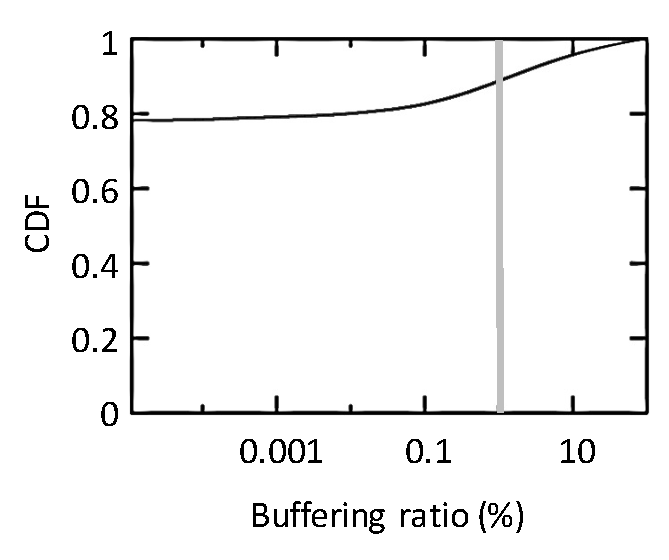
\includegraphics[width=0.35\textwidth]{figures/intro-badqoe-video-buffering.pdf}
%        \label{subfig:intro-badqoe-video-buffering}
%}
%%\hspace{-0.1cm}
%\subfloat[Internet telephony]
%{
%        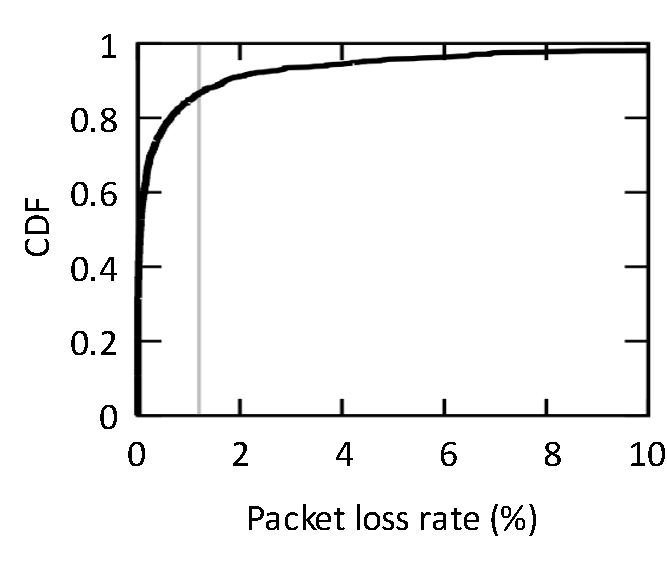
\includegraphics[width=0.35\textwidth]{figures/intro-badqoe-skype-lossrate.pdf}
%        \label{subfig:intro-badqoe-skype-lossrate}
%}
%%\vspace{-0.2cm}
%\caption{QoE distributions of video streaming and Internet telephony. 
%The figures shows that a substantial fraction of video sessions (12\%) 
%and VoIP calls (17\%) suffer from bad QoE (over 1\% buffering ratio 
%and 1.2\% packet loss rate, respectively).
%Buffering ratio is the fraction of video session duration spent in 
%re-buffering (video stalls), and is one of the key metrics of video 
%streaming QoE. 
%Packet loss rate is calculated over the call's duration, and is shown to 
%have significant impact on VoIP user experience.}
%%\vspace{-0.1cm}
%\label{fig:intro:badqoe}
%\end{figure}

\mypara{Limitations of prior approaches} 
These QoE problems stem from fundamental limitations of prior approaches. 
There are two broad categories of prior approaches, with the key difference 
lying in ``{\em where to implement the functionality of QoE optimization}''.

%To see why prior research has failed to deliver desirable 
%QoE in a substantial fraction of cases, one has to understand
%their fundamental limitations. 
%Prior networking approaches to Internet QoE optimization can be 
%classified to two broad categories depending on the answer to the key 
%architectural 
%question ``{\em where to implement the functionality of QoE optimization?}''


\begin{itemize}
\item On one hand, the {\em in-network approach} seeks to improve the 
quality of service of ISPs and middlebox services by better designs 
for in-network devices such as routers, switches and middleboxes.
%seeks to re-architect in-network devices such as routers, switches
%and middleboxes, so that ISPs can provide better or even guaranteed 
%quality of service. 
Although the  in-network approach has inspired influential projects 
(e.g.,~\cite{demers1989analysis,csfq,active-network}),
in-network devices have {\em limited visibility to user-perceived QoE}
as they have little access to the client-side applications.
Moreover, it is difficult, and increasingly so, to make substantial changes 
or add new services to the network core. 

\item On the other hand, the {\em endpoint approach} seeks to use
intelligent logic running at individual endpoints to adapt to dynamic
network conditions and fully utilize the existing network resources.
This approach is pervasively used in application-level protocols (e.g., video 
bitrate adaptation~\cite{dash}) and transport-level protocols (e.g., congestion 
control~\cite{jacobson1988congestion}).
While the endpoint approach has  direct insight to user-perceived QoE and is 
arguably more readily deployable than the in-network approach, 
it suffers from the key limitation that reacting to fluctuating network conditions based 
only on {\em local information} observed by individual endpoints could be suboptimal.
For instance, it takes a video player several seconds (sometimes, even tens of seconds)
to converge to an optimal combination of CDN and 
bitrate~\cite{dda}.
Moreover, we observe a growing decision space of potential control decisions 
to optimize application quality.
Therefore, it is untenable to use trial-and-error strategies driven by 
single-session feedback to find optimal decisions in the growing decision space. 
%Due to this limited knowledge of network conditions, it is difficult for 
%the endpoint adaptation to cope with the {\em growing decision space} 
%of potential control decisions to optimize application quality.

%of endpoint adaptation suffer from two limitations: 
%(1) it can only use the information visible to individual endpoint to react to dynamic network 
%conditions or resource availability,
%and (2) it typically uses manually designed strategies. 
%These two features inherently mismatch two recent trends of Internet applications
%First, we observe a {\em growing decision
%space} of potential control decisions to optimize application quality.
%Consequently, trial-and-error strategies driven by single-session feedback are
%fundamentally inefficient and slow in exploring the decision space and reacting to
%changes. For instance, it takes a video player several chunks (roughly 10s of
%seconds) to converge to an optimal combination of CDN and bitrate~\cite{dda-report}.
%Second,  we see an {\em increasing heterogeneity} in operating conditions, each requiring
%different control logic and parameters.  For instance, TCP parameters such
%as initial congestion window and AIMD parameters could be tweaked to work
%better in different operating conditions~\cite{remy,googleinitwindow}.
\end{itemize}

In essence, prior approaches to the placement of QoE optimization have to 
make trade-offs between
{\em visibility of user-perceived QoE} as feedback and {\em visibility of network conditions}, 
both of which, however, are critical to achieving desirable QoE in practice. 
In contrast, this dissertation approaches the placement of QoE optimization with a radically
different answer, and presents practical solutions to demonstrate that the new approach 
can get the best of both worlds.


\section{Data-Driven Paradigm in Networking}

This dissertation is inspired by a recent paradigm shift in networking research 
towards {\em Data-Driven Networking} ({\em \ddn}) -- network protocols should 
be driven not only by information available to one device, but by {\em real-time} 
information gathered from {\em multiple} devices, in order to adapt to changes 
in network conditions and resource availability.
Recent work has shown early promise of this paradigm shift in improving QoE of 
Internet applications (e.g.,~\cite{sigcomm12,footprint}).
The basic idea is to use a centralized controller to maintain a global view of 
network conditions based on QoE measured from many (typically, tens of 
thousands or more) of application sessions\footnote{We use ``client'' to denote 
where a ``session'' is actually run.} and use this real-time global view to make  
optimal decisions regarding configurations or adaptations of individual sessions.
A case in point is C3~\cite{c3}, where a video content provider 
collects session-level QoE measurements (e.g., buffering events) from 
the video players of its viewers, and predicts for any new session the best
bitrate and CDN selection based on the QoE measurements of 
history and concurrent video sessions.

%we can improve QoE by accurately predicting network conditions
%based on {\em a real-time, global view of QoE measured from millions of 
%end users~\cite{ddn-comsnet}.}


%\mypara{\ddn controller} 
%The key component in \ddn is a logically centralized 
%{\em controller}, which updates a real-time, 
%global view of network conditions by 
%QoE observed by applications running on 
%many end users in real time, and uses this global view of
%network conditions  to make  optimal decisions 
%regarding configurations or adaptations of clients or application 
%sessions\footnote{We use ``client'' to denote where a ``session'' 
%is actually run.}.


\begin{figure}[t!]
\captionsetup[subfigure]{justification=centering,farskip=-1pt,captionskip=5pt}
\centering
%\hspace{-0.5cm}
\subfloat[Classic approaches.]
{
        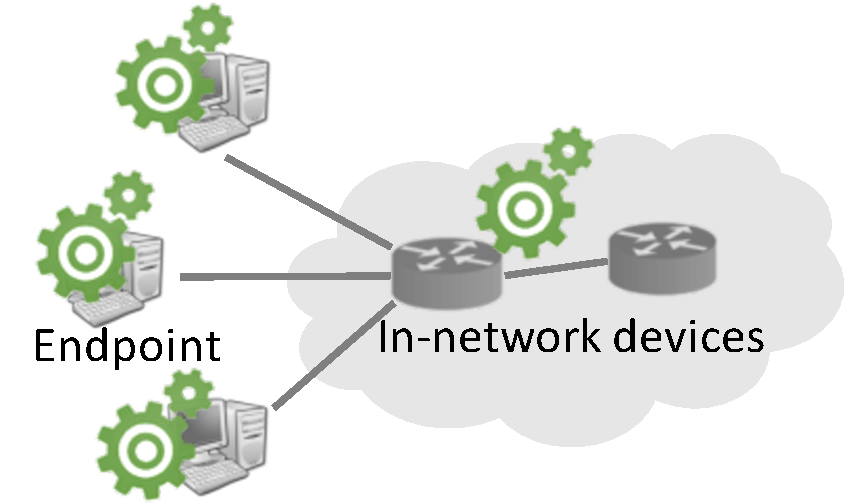
\includegraphics[width=0.4\textwidth]{figures/intro-classic.pdf}
        \label{subfig:problem-of-epsilon:change}
}
%\hspace{-0.1cm}
\subfloat[The new data-driven approach (\ddn).]
{
        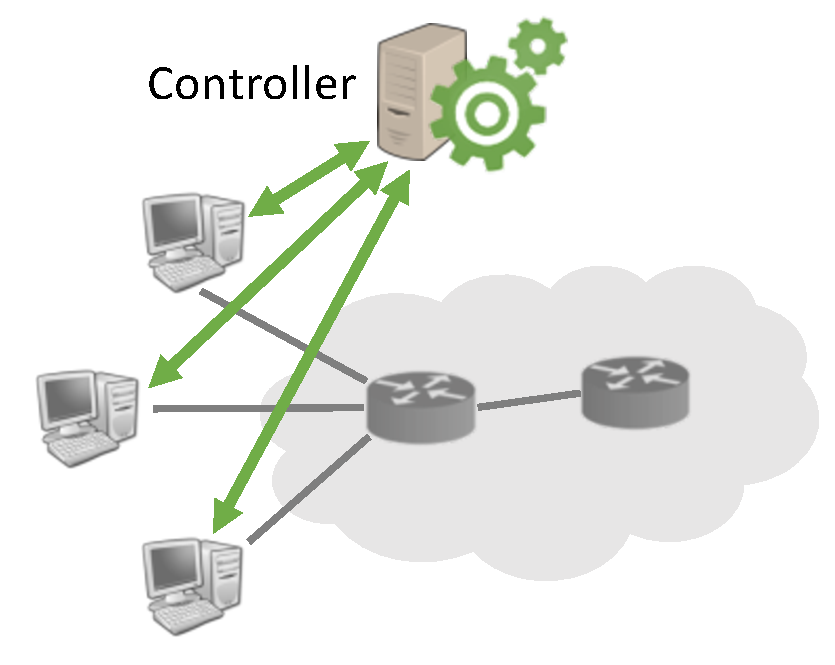
\includegraphics[width=0.4\textwidth]{figures/intro-ddn.pdf}
        \label{subfig:problem-of-slow:load}
}
%\vspace{-0.2cm}
\caption{Contrasting \ddn paradigm with classic approaches. 
The key distinction lies in where to implement the functionality of QoE optimization 
(symbolized by the gears): prior approaches implement 
it in the in-network devices or individual endpoints, whereas \ddn implements 
it in the controller that maintains a real-time global view of QoE of millions of endpoints.}
\vspace{-0.1cm}
\label{fig:intro:contrast}
\end{figure}

\mypara{Advantages of \ddn} 
The key advantage of \ddn over prior approaches is that 
\ddn retains the ethos of the endpoint approach, 
while addressing its lack of visibility to network condition by leveraging 
an expended view across many endpoints, thus achieving 
the best of both worlds of in-network and endpoint approaches.
As shown in Figure~\ref{fig:intro:contrast}, \ddn represents a new approach
to the architectural question: ``where to implement the functionality of QoE 
optimization''.
While the classic approaches implement QoE optimization in the network 
core or individual endpoints, \ddn implements it in the controller 
that maintains a real-time global view of QoE collected from
client-side applications running in millions of end users.
Moving the QoE optimization to the \ddn controller 
enjoys two key architectural advantages:
\begin{enumerate}
\item Unlike the in-network approach, \ddn can monitor client-side applications
and thus can directly optimize user-perceived QoE, rather than indirect metrics.
%as it has access to client-side applications,
Moreover, it is more readily deployable than the in-network approach.
\item Unlike the endpoint approach, \ddn compensates the lack of 
visibility of network conditions at one endpoint by a real-time, global view of QoE 
observed from many endpoints, thus addressing the key limitation of 
the endpoint adaptation. 
%Instead of reacting to dynamic network conditions with 
%a local view, \ddn can {\em predict}  the QoE that a session would 
%experience if it uses certain decision.
\end{enumerate}

%\mypara{Technology trends} 
\mypara{Technology push behind \ddn} 
%\vspace{0.2cm}
%\noindent{\bf Why now?}
Compared to its precursors (e.g.,~\cite{spand,seshan1997spand}),
\ddn is fortuitously aligned with several recent  ``technology pulls'':
\begin{enumerate}
\item Many application providers today have widely deployed client-side 
instrumentations to collect massive real-time in-situ QoE data  (e.g.,~\cite{sigcomm11,via,akamai-imc12,artizanetworks}). 
\item The emergence of large-scale analytics systems provides the ability 
to extract insights efficiently from large corpses 
of data (e.g.,~\cite{spark}) and from streams of updates 
(e.g.,~\cite{zaharia2013discretized}). 
%Such ability enables optimal decision making based on
%real-time data-driven predictions~\cite{velox-cidr}.
\item Control plane infrastructures have been built in many 
application providers (e.g., content providers~\cite{c3}, web services~\cite{footprint})
and infrastructure providers
(e.g., CDNs~\cite{chen2015end,mukerjee2015practical}).
\end{enumerate}

%\begin{itemize}
%\item {\em More measurement data in networking:}
%Many application providers today have widely deployed client-side 
%instrumentation to collect real-time performance data. 
%
%\item {\em ``Big data'' platforms finally a reality:}
%The emergence of large-scale analytics systems provides the ability to extract insights efficiently from large corpses 
%of data (e.g.,~\cite{spark}) and from stream of updates (e.g.,~\cite{dstream}). 
%Such ability enables optimal decision making based on real-time data-driven 
%predictions~\cite{velox}.
%
%\item {\em Wide use of control platforms:}
%Control plane platforms have been built by many individual subsystems (e.g., ISPs, video service providers and CDNs).
%
%\end{itemize}


%To take a concrete example, let’s think about Netflix player. 
%Traditionally, it takes a Netflix video player tens of seconds to converge to a good 
%quality, while in the new data-driven approach, Netflix can achieve much better 
%quality by using real-time quality measurement from many video players to directly 
%predict the best configuration for individual Netflix players.


%\subsection{Opportunities}

%\mypara{Opportunities of data-driven networking} 
%The data-driven approach is fortuitously aligned with several recent technology trends. Specifically, 
%
%\begin{itemize}
%\item {\em More measurement data in networking:}
%Many application providers today have widely deployed client-side 
%instrumentation to collect real-time performance data. \jc{examples}
%
%\item {\em ``Big data'' platforms finally a reality:}
%The emergence of large-scale analytics systems provides the ability to extract insights efficiently from large corpses 
%of data (e.g.,~\cite{spark}) and from stream of updates (e.g.,~\cite{dstream}). 
%Such ability enables optimal decision making based on real-time data-driven 
%predictions~\cite{velox}. \jc{examples}
%
%\item {\em Wide use of control platforms:}
%Control plane platforms have been built by many individual subsystems (e.g., ISPs, video service providers and CDNs). \jc{examples}
%
%\end{itemize}

\section{Roadmap of This Dissertation}

While prior studies did extrapolate potential improvement of \ddn, it is not 
clear how to fully realize its benefit in practice.
{\em The main contribution of this dissertation is the first suite of solutions 
to make \ddn practical}. In particular, 
%, and the demonstration that QoE of video streaming and Internet telephony can be 
%substantially improved by the application of \ddn.
%We demonstrate that QoE can be substantially improved by leveraging QoE 
%observed from millions of endpoints to maintain an up-to-date
%global view of network conditions.
%To achieve this, 
we identify key technical challenges of applying \ddn in to QoE optimization, 
address these challenges by novel algorithm and system designs that 
integrate machine-learning techniques with domain-specific  insights,
and use real-world deployment and large-scale 
emulation to demonstrate that our solutions can substantially improve 
QoE of video streaming and Internet telephony.
We will elaborate them in more details in Chapter~\ref{ch:overview}.

\subsection{Fundamental Challenges in Data-Driven Networking}
%While \ddn enjoys several advantages over 
%classic approaches, 
From our experience of applying \ddn in various applications, 
two fundamental challenges emerge as key to unleashing \ddn's full potential.
%We observe two fundamental challenges 
%that are key to unleashing \ddn's full potential.
%We focus on two fundamental challenges unique to \ddn:

\begin{enumerate}

\item 
%{\em The need for expressive models} to capture complex factors affecting QoE. 
{\bf Expressive models:} \ddn needs to extract actionable insights from the QoE measurement data, 
such as which sessions can be used to inform the decision of a new session.
%such as a predictive model to predict QoE based on session-level features, from 
%the data stream of QoE measurements. 
Thus, we need expressive models to capture the potentially complex 
factors affecting QoE. 

\item 
%{\em The need for scalable platforms} to make real-time decisions with fresh data from geo-distributed clients.
{\bf Scalable platforms:}
\ddn needs to turn the actionable insights into 
real-time control decisions to be performed by applications running in
geo-distributed clients. 
Therefore, we need that can respond to geo-distributed 
clients in real time with decisions based on fresh data from other clients.

\end{enumerate}

\subsection{Unifying Insight: Persistent Critical Structures}
This dissertation addresses these challenges by integrating 
machine learning techniques with
%As a result, our 
%solutions achieve better QoE 
%than using off-the-shelf machine learning solutions. 
the unifying insight that there are {\em persistent structures} in the relationship
between session-level features, decisions, and QoE.
At a high level, these structures have two distinctive features:
%(1) they help identify network sessions with similar 
%QoE-determining factors, and (2) they tend to persist on timescales of tens of minutes.
(1) they allow us to build expressive models that can identify network 
sessions with similar QoE-determining factors, and 
(2) because these structures are persistent, we can 
build scalable systems by decoupling the offline structure-learning 
process and the real-time decision making process.
To see an intuitive example of these persistent structures, let us consider 
a group of video sessions bottlenecked by a congested link.
The quality of these sessions may vary over time, but the fact
that these video sessions are bottlenecked by the same congested link remains true 
for the whole duration of the congestion event.
In this example, the correlation among the quality of these sessions 
is a persistent structure, which manifests the underlying congestion.
We will give a formal definition of persistent structures in
Section~\ref{sec:overview:unifying}.


%\section{Contributions}



%\mypara{Challenges}
%While \ddn enjoys several advantages over 
%classic approaches, we observe two fundamental challenges 
%that are key to unleashing \ddn's full potential.
%%We focus on two fundamental challenges unique to \ddn:
%
%\begin{enumerate}
%
%\item 
%%{\em The need for expressive models} to capture complex factors affecting QoE. 
%First, \ddn needs to extract actionable insights from the QoE measurement data, 
%such as which sessions can be used to inform the decision of a new session.
%%such as a predictive model to predict QoE based on session-level features, from 
%%the data stream of QoE measurements. 
%In short, we need {\em expressive models} to capture the potentially complex 
%factors affecting QoE. 
%
%\item 
%%{\em The need for scalable platforms} to make real-time decisions with fresh data from geo-distributed clients.
%Second, \ddn needs to turn the actionable insights into 
%real-time control decisions to be performed by applications running in
%geo-distributed clients. 
%Therefore, we need {\em scalable platforms} that can respond to geo-distributed 
%clients in real time with decisions based on fresh data from other clients.
%
%\end{enumerate}

%\mypara{Key insight}
%In this dissertation, we address these challenges in practice by integrating 
%several domain-specific insights in networked applications with 
%standard machine learning algorithms and systems. 
%%As a result, our 
%%solutions achieve better QoE 
%%than using off-the-shelf machine learning solutions. 
%The unifying theme underlying these domain-specific insights is 
%that there are {\em persistent structures} in the relationship
%between session-level features, decisions, and QoE.
%These structures help identify network sessions with similar 
%QoE-determining factors, and that such structures tend to be 
%persistent on timescales of tens of minutes.
%To see an intuitive example of these persistent structures, let us consider 
%a group of video sessions bottlenecked by a congested link.
%The throughput of these flows may vary over time, but the fact
%that these video sessions are bottlenecked by this congested link remains true 
%for the whole duration of the congestion event.
%In this example,  the persistent correlation between these sessions' 
%network path and their QoE is a manifestation of the underlying congestion.
%We will give a formal definition of persistent structures in
%Section~\ref{sec:overview:unifying}.



%\begin{table}[]
%\centering
%\begin{tabular}{lll}
%\\ \hline
%{\bf Challenges} & {\bf Key ideas} & {\bf Published work}        \\ \hline\hline
%\begin{tabular}[c]{@{}l@{}}{\em Expressive models} for complex \\ QoE-determining factors\end{tabular}            & \begin{tabular}[c]{@{}l@{}}Use structures to identify sessions \\ with similar QoE-determining factors\end{tabular} & \begin{tabular}[c]{@{}l@{}}CFA~\cite{cfa}, VIA~\cite{via},  \\ CS2P~\cite{cs2p}\end{tabular}         \\ \hline
%\begin{tabular}[c]{@{}l@{}}{\em Scalable platforms} for real-time \\ decision making with fresh data\end{tabular} & \begin{tabular}[c]{@{}l@{}}Decouple offline structure learning \\ and the real-time decision making\end{tabular}    & \begin{tabular}[c]{@{}l@{}}Pytheas~\cite{pytheas}, CFA~\cite{cfa},  \\ C3~\cite{c3}, VDN~\cite{mukerjee2015practical}\end{tabular}\\ \hline
%\end{tabular}
%\caption{Summary of how the insight of persistent structures is used to address 
%the two key technical challenges of data-driven QoE optimization. The last 
%column shows the published work corresponding to these ideas.}
%\label{tab:contributions}
%\end{table}

\begin{figure}[t!]
\centering
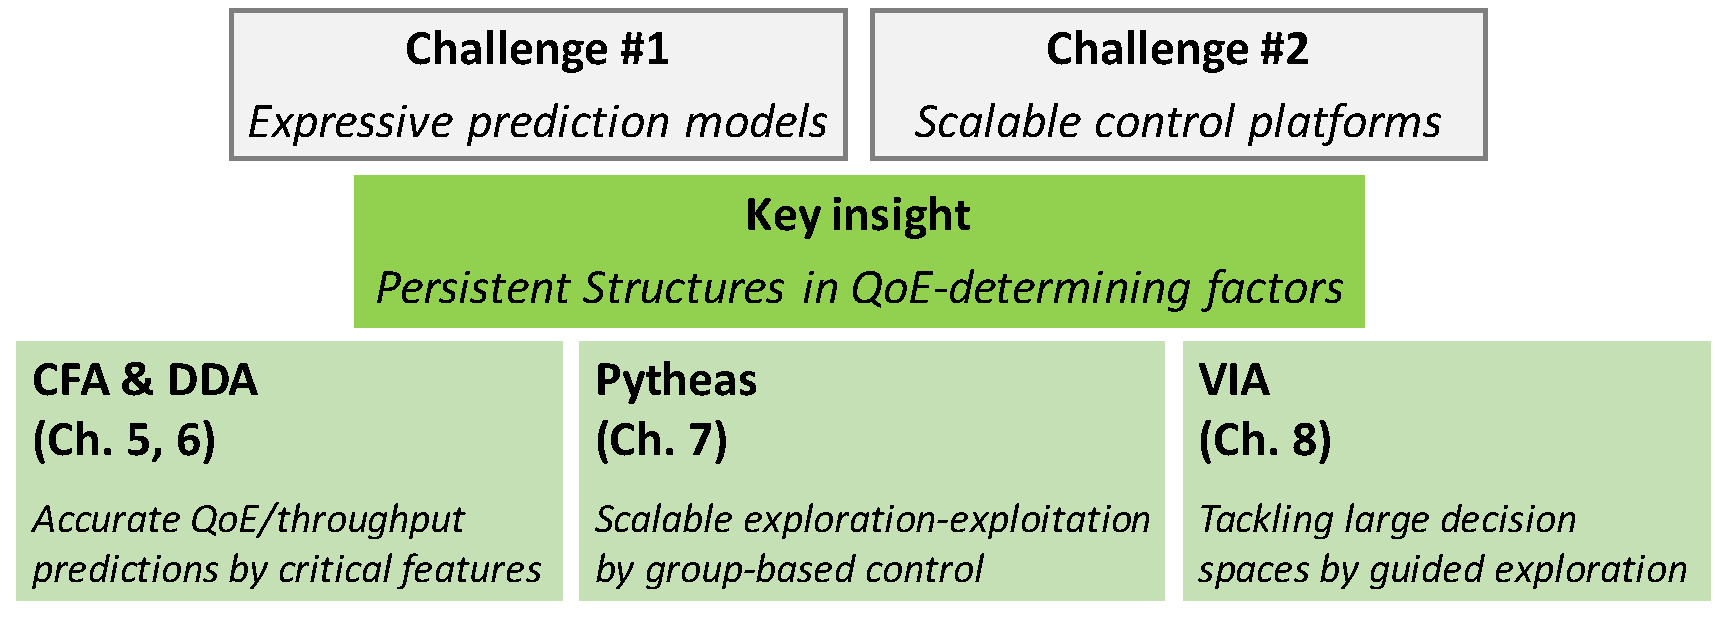
\includegraphics[width=0.8\textwidth]{figures/intro-contribution.pdf}
%\vspace{-0.3cm}
\caption{The main contribution of this dissertation is to present the first suite of 
solutions (bottom) to address the key challenges of \ddn (top) by leveraging the 
unifying insight (middle) that QoE-determining factors exhibit persistent structures.}
\label{fig:intro-contribution}
\end{figure}


\subsection{Proposed Solutions}
%\mypara{Proposed solutions}
%Table~\ref{tab:contributions} 
As illustrated in Figure~\ref{fig:intro-contribution}, 
the insight of persistent structures inspires the three concrete solutions
%of this dissertation.
to address the two aforementioned challenges in the context
of two popular Internet applications: Internet video and Internet telephony. 
%Based on these ideas, this dissertation has developed novel algorithms 
%and end-to-end systems, and deployed them in production settings to 
%improve QoE for Internet video streaming
%and Internet telephony. 
Next, we briefly describe the three components that constitute 
this dissertation.



\begin{itemize}

\item {\bf Improving video QoE via expressive prediction models} 
(Chapter~\ref{ch:cfa} and~\ref{ch:dda}). 
Prior work has shown a substantial room for improving video QoE by 
dynamically selecting the optimal CDN and bitrate for individual video 
sessions based on a real-time global view of network 
conditions~\cite{sigcomm12}.
To realize this promise, we have developed CFA~\cite{cfa}, a video QoE prediction 
system that can accurately predict the quality of a video client if it uses 
a certain CDN and bitrate; and DDA~\cite{dda}, a throughput prediction system
to accurately predict end-to-end throughput at the beginning of a 
 video session to help determine the highest-yet-sustainable initial bitrate.
In particular, CFA is inspired by the domain-specific insight of 
{\em persistent critical features}, an instantiation of persistent structures, that
each video session has a small set of critical features that ultimately 
determines its video quality, and these critical features change much 
more slowly than video quality, and thus can be practically 
learned from history data.
%This insight enables us to learn complex prediction models from long-term historical data (thus expressing complex relations between video quality and session features), and update the models by short-term historical data in near real time (thus capturing quality fluctuation as well).
%The insight of persistent critical features turns out to be more general than video streaming; e.g., I have also applied the same insight to accurate prediction of TCP throughput~\cite{cs2p}, which leads to 11\% higher video bitrate than state-of-the-art adaptive bitrate players (e.g., Netflix players) with no extra buffering.

\item {\bf Improving video QoE via exploration and exploitation at scale} 
(Chapter~\ref{ch:pytheas}). 
While CFA and DDA show promising QoE improvement by formulating the 
data-driven QoE optimization as a prediction problem, this formulation is necessarily 
incomplete, as it suffers from many known biases such as incomplete visibility, 
and cannot respond to sudden changes such as flash crowds.
Drawing a parallel from machine learning (e.g., ad recommendation), 
we argue that data-driven QoE optimization should instead be 
cast as a process of {\em real-time exploration and exploitation}. 
To apply this new abstraction to network applications at scale, 
we develop an end-to-end system, called Pytheas~\cite{pytheas}, based on 
another illustration of persistent structures that 
the sessions that exhibit similar QoE behavior will have similar network-level 
features (e.g., IP prefix), and thus their fresh data could be collected 
by the same geo-distributed front-end cluster close to the clients of
these sessions. Inspired by this insight, Pytheas uses a scheme called 
{\em group-based exploration and exploitation},  which decomposes the 
global exploration and exploitation process into 
subprocesses, each of which runs in a geo-distributed front-end cluster 
 and makes real-time decision for a group of similar sessions
based on their fresh measurement data.

\item {\bf Improving Internet telephony QoE in the face of large decision spaces} 
(Chapter~\ref{ch:via}).
The last project tackles a challenge of large decision spaces, which 
is particularly relevant in Internet telephony.
In the first large-scale study on VoIP\footnote{We use the terms Internet telephony 
and VoIP interchangeably.} quality, we found that 
%a substantial fraction of Skype calls suffer from poor network performance, 
%and that 
there is substantial room for improving Skype quality by routing each 
call through the optimal relay clusters in Microsoft's cloud.
However, identifying a close-to-optimal relay for each Skype call in practice 
is challenging, 
due to the sheer number of possible relay paths 
(in hundreds) and their dynamic performance (which could change 
on timescales of minutes). Neither prediction-based methods (e.g., 
CFA) nor those based on 
exploration and exploitation (e.g., Pytheas) would suffice to handle such a 
large decision space.
Our key insight to address this challenge is that, for each pair of caller 
AS and callee AS, there is a {\em small and stable subset} of relays that 
almost always contains the best relay path. These stable subsets of promising
relays are another manifestation of the persistent structures.
%This insight has two implications: 
%(1) because this subset of relays is stable, it can be learned from history; and 
%(2) because this subset has only a few relays (less than five), it can be explored efficiently even with limited data.
Inspired by these intuitions, we developed {VIA}~\cite{via}, 
a Skype relay selection system that achieves close-to-optimal quality 
using the concept of {\em guided exploration},
which learns a small set of promising relays for each 
AS pair based on long-term (e.g., daily) historical data, and 
explores these relays using most calls in real time.

\end{itemize}


%
%\jc{add why internet video, voip, and how to generalize}
\mypara{Generalizability of the proposed solutions}
Finally, while this dissertation has mostly focused on 
Internet video and Internet telephony, 
we observe similar data-driven opportunities in other applications
where solutions proposed in this dissertation can be readily 
deployable; e.g., CDN overlay routing~\cite{mukerjee2015practical}, 
web services~\cite{footprint}.
%some of which I have personally involved as well.
%We also observe parallel efforts that hint towards the potential
%of using a similar data-driven approach in other applications, such
%as web services~\cite{footprint}.
This suggests the potential {\em generalizability} of our solution to enable
data-driven QoE optimization in a broader set of challenges in 
networking and distributed systems.
%for particular applications might be 
%{\em generalized} to other applications and potentially to solutions for
%a broader set of challenges in networking and distributed systems.

%\subsection{Evaluation}
%These improvements can lead to significant benefit for the application providers.





%\mypara{Deployment}

\subsection{Summary of results}
%In order to evaluate the solutions proposed in this dissertation, 
%I focus on answering the following questions. 
In evaluating the solutions proposed in this dissertation, 
we focus on answering two questions.

\begin{itemize}

\item {\em How much can QoE be improved by the proposed solutions?}
The ultimate goal of \ddn is to improve QoE. 
Rather than evaluating multiple solution together, we examine the 
contribution of each solution by evaluating the incremental QoE 
improvement of adding one component at a time. 
For instance, by predicting the best CDN and bitrate selections based on 
a global view of network conditions, CFA reduces video re-buffering time 
on average by 32\% compared to a state-of-the-art client-side logic using 
local information (Chapter~\ref{ch:cfa});
and by re-casting the data-driven QoE optimization as a real-time 
exploration-and-exploitation process, Pytheas further reduces the 
re-buffering time on average by 30\% over CFA (Chapter~\ref{ch:pytheas}).
In Chapter~\ref{ch:via}, we show that VIA achieves better VoIP QoE
than CFA and Pytheas
by addressing the new challenge of large decision spaces in
Internet telephony.
Moreover, this dissertation also tries to identify the circumstances under which
the proposed solutions achieve more (or less) QoE improvement.
For instance, in Chapter~\ref{ch:via}, while 
we observe significant improvement of 
VIA on both international and domestic Skype calls, international calls
have a higher magnitude of improvement than domestic ones.

%Chapter~\ref{ch:cfa} shows that by predicting the best 
%CDN and bitrate selections based on a real-time, global view of network 
%conditions, CFA reduces re-buffering time on average by 32\% compared 
%with those selections made by a state-of-the-art client-side logic using 
%local information.
%Then Chapter~\ref{ch:pytheas} shows that Pytheas can further reduce the 
%re-buffering time on average by 30\% over CFA by recasting the 
%data-driven QoE optimization as a 
%real-time exploration-and-exploitation process.
%Finally, in Chapter~\ref{ch:via}, we show that VIA achieves better QoE
%than CFA and Pytheas in the context of a VoIP service 
%by reducing large decision spaces unique to Internet telephony.


\item {\em Can the proposed solutions be deployed at a real scale?}
Scalability is another critical metric to evaluate the proposed solutions. 
Any proposed algorithm must run at the scale of a large application 
provider.
%(e.g., YouTube has billions of video sessions per
%day over the world~\cite{youtube-stats}).
This means that the decisions must be made 
based on history data at a magnitude of hundreds GB or more, and 
these history data from geo-distributed 
clients must be up-to-date to maintain an accurate view of network conditions.
In Chapter~\ref{ch:cfa}, we show that CFA can update QoE 
prediction every tens of seconds with sub-second response 
time to geo-distributed clients, 
and in Chapter~\ref{ch:pytheas}, we show that Pytheas throughput 
scales horizontally with more machines in the controller, and that 
30 CloudLab instances can make decisions for the population of a site
like YouTube (5 billion sessions per day) with measurement data of 
concurrent sessions with less than a second of delay.

\end{itemize}


%\mypara{Evaluation methodology}
%\mypara{Dataset}
To demonstrate the benefit of our solutions in realistic settings, 
our evaluation methodology combines real-world pilot deployment and 
emulation/simulation driven by large-scale datasets collected from real  users.
%this dissertation relies on either real-world pilot deployment or emulation 
%driven by large-scale datasets collected from real application traffic.
For instance, in Chapter~\ref{ch:cfa}, we integrated CFA in a production 
system~\cite{c3} that provided video optimization service for major content
providers in the US.
%to select CDNs and bitrates for real users for one of the biggest
%content providers in the US. 
We deployed CFA on one of these content providers to improve QoE for
150,000 sessions each day. We performed A/B tests (where each algorithm
was used on a random subset of clients) to evaluate
the improvement of CFA over baseline random decision
makers, which many video optimization services use 
by default (modulo business arrangement like price).
%
%\mypara{Evaluation metrics} 
In order to evaluate application QoE in a reliable 
and scalable fashion, this dissertation does not rely subjective QoE 
metrics (e.g., user-provided score), but focus on the metrics that can be
objectively measured and 
have been shown to have strong impact on user satisfaction 
and engagement.
For instance, video QoE is measured by buffering time, start-up delay,
and average bitrate, each of which has been shown to have strong
correlation with user engagement in multiple 
studies~\cite{sigcomm11,akamai-imc12}.
While subjective metrics can directly reflect user satisfaction, we
choose to use these objectively measurable 
metrics as a proxy for real user satisfaction for two reasons:
(1) they can be passively collected on a large scale by instrumentation code 
running in client devices without any user input, and (2) they usually
are less noisy than subjective metrics which can be affected by factors
beyond the scope of this dissertation (e.g., content or personal preference).

%The QoE metrics against which different systems are compared 
%are objectively measurable metrics
%depend on the particular application under consideration.



\section{Organization}
The rest of this dissertation is organized as follows.
Chapter~\ref{ch:related} begins with the background information of
Internet video and Internet telephony, including their QoE problems
today and current distribution infrastructures.
It then discusses two research directions closely 
relevant to this dissertation: 
quality optimization of Internet applications and applying data-driven 
techniques in networked systems.
In particular, it introduces a taxonomy of prior work on quality 
optimization, which emphasizes the trade-offs between 
more visibility of QoE feedback and more visibility of network
conditions.

Chapter~\ref{ch:overview} presents an overview of the main insight and 
ideas of this dissertation.
It begins with a formal description of the \ddn paradigm, some
concrete example applications that can benefit from \ddn, and a
perspective on its advantages over prior approaches.
It then elaborates the key technical challenges in making \ddn practical. 
Finally, it describes our key insight of persistent structures in 
QoE-determining factors, and how the insight inspires our ideas to 
address \ddn's challenges.
%It concludes with the contrast between the proposed solutions and classic 
%approaches, in order to elaborate their advantages and limitations.

Chapter~\ref{ch:measurement} presents a large-scale structural analysis
on the QoE problems of Internet video and Internet telephony in the wild.
It provides empirical evidence of the persistent structures in QoE-determining
factors. 

Chapters \ref{ch:cfa}, \ref{ch:dda}, \ref{ch:pytheas}, and \ref{ch:via} 
describe four important components of this dissertation: 
(1) CFA and DDA optimize video streaming quality by accurately predicting 
video QoE and end-to-end throughput using a global and real-time view of 
network conditions;
(2) Pytheas optimizes quality of Internet-scale applications by re-casting
the \ddn process as a real-time exploration-exploitation process 
over millions of geo-distributed clients at scale; and
(3) VIA optimizes network performance for Skype calls by selecting
the optimal relay clusters in the Microsoft cloud service.

Chapter~\ref{ch:concl} summarizes the contributions of the dissertation, 
discusses the limitations of the proposed solutions, and ends with future 
work.












\chapter{Background}
\label{ch:related}

%\begin{itemize}
%\item internet app is important, and more so recently
%\item some applications are dominant in terms of traffic volume, number of flow, and indespensity.
%\end{itemize}
%
%\begin{itemize}
%\item long history of research efforts
%\item change the core
%\item moving to the edge
%\item data-driven
%\end{itemize}
%
%\begin{itemize}
%\item this chapter describe architecture and related work
%\end{itemize}

Before we embark on the solutions to improve QoE, it would be helpful
to (1) motivate the need for improving QoE by shedding
light on today's QoE problems in the wild, and (2) understand the 
fundamental trade-offs in prior approaches to QoE optimization.

%as well as prior efforts towards improving application QoE.
The first part of this chapter uses empirical measurement studies to 
show that there is a substantial fraction of sessions in both Internet 
video and Internet telephony with bad QoE  
(Section~\ref{sec:related:qoe}), and then discusses 
some salient aspects of distribution infrastructures of these
applications today (Section~\ref{sec:related:back}).
%we begin with  some background information on
%Internet video and Internet telephony (Section~\ref{sec:related:back}).

The second part of this chapter discusses two research directions, 
which are closely related to this dissertation:
optimization of Internet applications quality and network performance
(Section~\ref{sec:related:quality}) and application of data-driven 
techniques to improve networked systems (Section~\ref{sec:related:data}). 
In particular, it presents a taxonomy of prior approaches to QoE optimization, 
which emphasizes the fundamental trade-off between visibility to 
user-perceived QoE and visibility to network conditions.
%these prior efforts into perspective, and
The taxonomy also helps to crystallize the contrasts between
prior work and this dissertation (Section~\ref{subsec:overview:contrast}).

\section{How Good is QoE Today?}
\label{sec:related:qoe}

We begin with large-scale measurement studies based on QoE observed 
by real users to shed light on the how good (or bad) QoE is today for 
Internet video (Section~\ref{subsec:related:video-qoe}) and Internet telephony 
(Section~\ref{subsec:related:voip-qoe}) in the wild. 
For each application, we first introduce the QoE metrics 
and the dataset, and then present empirical session-level QoE distributions
for different quality metric.

\subsection{Video QoE}
\label{subsec:related:video-qoe}

\mypara{Video QoE metrics}
We focus on  four key video QoE metrics that are common across 
different  content providers and have been shown to be
 critical for measuring quality as well as user  engagement: 
\begin{packedenumerate}

\item \emph{Buffering ratio:}  Given a video session of 
duration $T$~seconds,  if the player spent $B$~seconds in 
buffering (i.e., waiting for the 
 buffer to replenish), the buffering ratio is defined as 
 $\frac{B}{T}$. 
 Prior work has shown that buffering ratio is a key metric
 that impacts user engagement~\cite{sigcomm11}.

\item \emph{Join time:}  This is the time taken for the video 
to start playing  from the time the user clicks on the ``play'' 
button. 
While join time may not directly impact the view time of a 
specific video,
it does have long-term effects as it reduces the likelihood 
of repeated visits~\cite{sigcomm11,akamai-imc12}.  
 

\item \emph{Average bitrate:} 
Many video players today support adaptive bitrate
selection and midstream bitrate switching to adapt to 
changing bandwidth availability. 
The average bitrate of a session is the time-weighted
average of the bitrates used in a given video session. 


\item \emph{Join failures:}   Some sessions may not even 
start playing the video; either the content is not available
 on the CDN server or the CDN is under overload or other 
unknown reasons. We mark such a session as a join failure
if no content was played during this session.

\end{packedenumerate}


\mypara{Dataset} 
Our dataset is based on client-side measurements of
video  quality from over 300 million sessions over a duration
of two weeks. The unique feature of our dataset is that it is 
collected over 379 distinct content providers spanning diverse 
genres, both live and video-on-demand content, different 
content delivery platforms, different types of  bitrate adaptation 
algorithms, and device/browser platforms. 
Though US viewers dominate the dataset ($\sim$55\%), 
there are a fair number of European ($\sim$12\%) and 
Chinese ($\sim$8\%) users in the dataset.
This is especially relevant as it provides us with a panoramic 
view   of state of  Internet video delivery today.
More details on the datasets can be found in~\cite{jiang2013shedding}.

\begin{figure*}[t]
\centering
\captionsetup[subfigure]{justification=centering,farskip=-1pt,captionskip=5pt}
\subfloat[Buffering ratio]{
   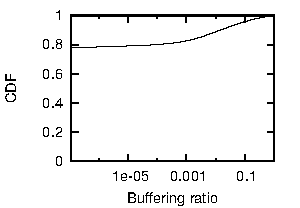
\includegraphics[width=0.32\textwidth] {figures/value_buffering.pdf}
 }
\subfloat[Bitrate]{
   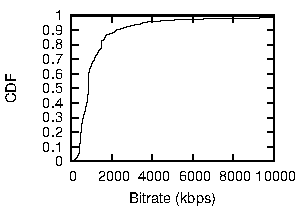
\includegraphics[width=0.32\textwidth] {figures/value_bitrate.pdf}
 }
\subfloat[Join time]{
   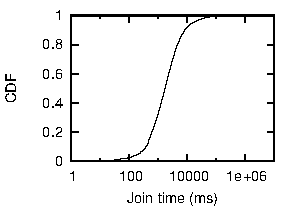
\includegraphics[width=0.32\textwidth] {figures/value_jointime.pdf}
 }
\caption{Distributions of observed video QoE metrics -- 
buffering ratio, average bitrate, and join time. 
 We see that a non-trivial number of sessions suffer quality problems. 
 For instance, more than 5\% of sessions have a buffering ratio larger
  than 10\%.  }
\label{fig:overview:qualitycdf}
\end{figure*}

\mypara{QoE distributions of different metrics}
Figure~\ref{fig:overview:qualitycdf} shows the distributions of the 
first three quality metrics over the dataset.  
(Join failures are binary events; it is not meaningful to look at a 
distribution.) 
The results reconfirm prior observations that there are a non-trivial 
number of sessions with less-than-ideal 
quality~\cite{sigcomm11,sigcomm12}. 
The key difference here is that  these past efforts only considered 
a small set of 3--4 content providers. 
In contrast,   we are considering the aggregate data from over 
300 content providers, and our results suggest that the QoE 
problems might be more pervasive than what we realized.
For instance, more than 5\% of all sessions have a join time greater 
than 10~seconds; i.e., users had to wait for 10 seconds before the 
video even started playing! Similarly, more than 5\% of sessions 
had a buffering ratio that was greater than 10\%.  
This is particularly bad as past studies show that even a 1\% 
increase in buffering ratio can lead to 3-4 minutes of lost 
viewership~\cite{sigcomm11}.  
Finally, we also see that more than 80\% of sessions observe 
an average  bitrate less than 2~Mbps; 
i.e., less than the lower end of today's ``HD'' content.   
Note that the dataset from which these observations are made
is dominated by  US-based content providers where viewers in general
have good broadband penetrations, so QoE could be even worse in 
other less developed regions.
%less than the lower end of 
%today's ``HD'' content.  





\subsection{VoIP QoE}
\label{subsec:related:voip-qoe}

\newcommand{\Call}{\ensuremath{c}\xspace}
\newcommand{\CallSet}{\ensuremath{C}\xspace}
\newcommand{\Relay}{\ensuremath{r}\xspace}
\newcommand{\RelaySet}{\ensuremath{R}\xspace}
\newcommand{\QualityFunc}{\ensuremath{Q}\xspace}
\newcommand{\HistoryCallSet}{\ensuremath{H}\xspace}
\newcommand{\Assign}{{\sf\small Assign}\xspace}
\newcommand{\Budget}{\ensuremath{B}\xspace}
\newcommand{\Predictor}{{\sf\small Pred}\xspace}
\newcommand{\BuildPredictor}{{\sf\small BuildPredictor}\xspace}
\newcommand{\GetTopK}{{\sf\small GetTopK}\xspace}
\newcommand{\Explore}{{\sf\small Explore}\xspace}
\newcommand{\Src}{\ensuremath{s}\xspace}
\newcommand{\Dst}{\ensuremath{d}\xspace}

\newcommand{\hybrid}{\textsc{Via}\xspace}
\newcommand{\Name}{Via\xspace}

\newcommand{\skype}{{Skype}\xspace}
\newcommand{\azure}{{ABC}\xspace}
\newcommand{\direct}{{default}\xspace}
\newcommand{\option}{{relaying option}\xspace}
\newcommand{\options}{{relaying options}\xspace}

\begin{figure}[t!]
\centering
\subfloat[\small{PCR vs. RTT (0.97)}]
{
        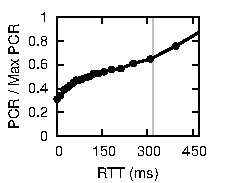
\includegraphics[width=0.3\textwidth]{figures/Via-Quality-vs-Pcr-RTT.pdf}
        \label{subfig:pcr-rtt}
}
\subfloat[\small{PCR vs. Loss (0.95)}]
{
        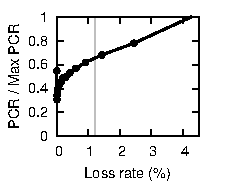
\includegraphics[width=0.3\textwidth]{figures/Via-Quality-vs-Pcr-Loss.pdf}
        \label{subfig:pcr-loss}
}
\subfloat[\small{PCR vs. Jitter (0.91)}]
{
        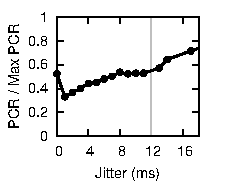
\includegraphics[width=0.3\textwidth]{figures/Via-Quality-vs-Pcr-Jitter.pdf}
        \label{subfig:pcr-jitter}
}
\caption{Network performance metrics have considerable 
impact on VoIP QoE (poor call rate or PCR); 
y-axis normalized to the maximum PCR. Vertical gray lines 
show the thresholds for poor network performance. Numbers in the
brackets show the correlation coefficients.}
\label{fig:pcr}
\end{figure}

%To quantify the call quality, we first consider an empirical approach. 
\mypara{VoIP QoE metrics}
Like video QoE metrics, VoIP QoE ideally should be based on some 
user-provided scores, but getting such information directly from users 
is not scalable.
Fortunately, for a small random fraction of calls in \skype, 
users label the call quality on a discrete $5$-point scale, 
ranging from $1$ 
(worst) to $5$ (best). This allows us to study the correlation
between these user-provided scores and network metrics that 
can be objectively measured in a scalable fashion. 
We can then use these network metrics to study the QoE 
problems across a large number of users.

Consistent with the operational practice in \skype, we deem 
the calls with a rating of $1$ or $2$ as ``poor'', and use the 
fraction of such calls, termed as the {\em Poor Call Rate (PCR)}, 
as an empirical metric of QoE. 
Figure~\ref{fig:pcr} shows the impact of the three network 
performance metrics (RTT, loss rate, jitter) on the (normalized)
user-derived PCR\footnote{Besides PCR, 
prior work also has provided analytical models to 
translate the network metrics into a measure of audio call quality, 
called the {\em Mean Opinion Score (MOS)} (e.g., \cite{cole}). 
Our study also showed that MOS is similarly correlated with
these network metrics~\cite{via}.}. 
For each network metric, we bin calls based on their 
network performance and show the PCR of the calls within 
each bin. 
For statistical significance, each bin has at least $1000$ samples. 
The figures show PCR significantly increases with all the three 
network metrics (correlation coefficients of $0.97$, $0.95$, $0.91$), 
confirming that user-perceived quality is indeed sensitive to 
network performance.
Interesting, PCR is sensitive to the {\em entire} spectrum of 
network metrics. This suggests that any improvement in RTT, 
loss or jitter is likely to improve PCR.


\mypara{Dataset}
The dataset from \skype consists of a sampled set of $430$ 
million audio calls drawn from a seven month period. 
%\camera{They are sampled from \cmvnp{the set of} calls made by \cmvnp{clients on the} \fillme platform \cmrvnp{and they are the only calls with recorded} \cmvnp{and for which} performance metrics \cmvnp{are recorded}.}
%\vnp{I wonder if the low count is because we are only considering calls for which the performance metrics are recorded. If so, we should say so.} 
The sampled set includes both calls that use the 
\direct path (e.g., BGP-derived) between the caller 
and the callee %(\cameraremove{$40\%$}\camera{$15\%$} of the calls in the set) 
as well as calls that are relayed through managed 
relay nodes distributed across datacenters in different 
locations. % (the remaining \cameraremove{$60\%$}\camera{$85\%$} of the calls). 
%\vnp{We say "randomly sampled" and then also say "sampled set is chosen" (which appears to contradictory to "random") and furthermore give the 40-60 split (which, together with "random", leaks info on how much relaying happens). I would suggest striking off "randomly".} 
Note that today such relaying is typically employed for 
connectivity (e.g., firewall or NAT traversal);
%rather than 
%for performance optimization (which is our focus here).
i.e., the only instances of relaying in our passively 
collected dataset correspond to the caller and callee being 
unable to establish a direct connection. 
Despite this bias, the dataset offers a {\em panoramic} view 
across diverse end-points from $1,905$ ASes across $126$ 
countries. 
%Table~\ref{tab:dataset} summarizes the statistics.
% \footnote{In general, it is unclear if reachability and performance are correlated.}



%In this section, we show that PCR\footnote{Besides PCR, 
%prior work also has provided analytical models to 
%translate the network metrics into a measure of audio call quality, 
%called the {\em Mean Opinion Score (MOS)} (e.g., \cite{cole}).} is
%well-correlated with network metrics. 
%Then, we identify suitable {\em thresholds} for poor call 
%performance on the network metrics of RTT, loss and jitter. 
%Since our goal is to understand the impact of network 
%performance metrics on call quality, the thresholds keep 
%our focus directly on these network metrics.
%
%\mypara{Does network performance impact user experience?}
%Figure~\ref{fig:pcr} shows the impact of the three network 
%performance metrics (RTT, loss rate, jitter) on the (normalized)
%user-derived PCR. 
%For each network metric, we bin calls based on their 
%network performance and show the PCR of the calls within 
%each bin. 
%For statistical significance, each bin has at least $1000$ samples. 
%The figures show PCR significantly increases with all the three 
%network metrics (correlation coefficients of $0.97$, $0.95$, $0.91$) 
%confirming that user-perceived quality is indeed sensitive to 
%network performance.
%Interesting, PCR is sensitive to the {\em entire} spectrum of 
%network metrics. This suggests that any improvement in RTT, 
%loss or jitter is likely to improve PCR.
%%Figure~\ref{fig:mos} shows the impact of RTT, loss rate, and jitter on MOS. %This is just a depiction of the relationship captured in the MOS equation noted above. 
%MOS (calculated using the model in \cite{cole}) also drops 
%with increase in all three metrics.

%\mypara{QoE distribution}
%We define the {\em poor network rate} (PNR) of a network 
%metric for a set of calls as the fraction of calls whose performance 
%on the metric is worse than the chosen thresholds: 
%RTT $\geq 320$ms, loss rate $\geq 1.2\%$, jitter $\geq 12$ms. 
%One of our goals is to reduce PNR of {\em each} individual metric 
% (i.e., how often each of them is poor). 


\begin{figure}[t!]
\centering
\subfloat[\small{RTT}]
{
        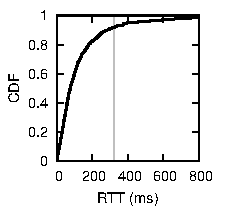
\includegraphics[width=0.28\textwidth]{figures/Via-Quality-CDF-RTT.pdf}
        \label{subfig:}
}
\subfloat[\small{Loss}]
{
        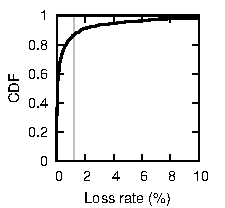
\includegraphics[width=0.28\textwidth]{figures/Via-Quality-CDF-Loss.pdf}
        \label{subfig:}
}
\subfloat[\small{Jitter}]
{
        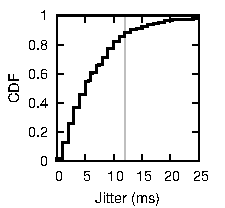
\includegraphics[width=0.28\textwidth]{figures/Via-Quality-CDF-Jitter.pdf}
        \label{subfig:}
}
\caption{Distributions of observed network performance metrics of Skype calls -- 
RTT, loss rate, jitter. Vertical grey lines show the thresholds 
for poor network performance.}
\label{fig:perf-cdf}
\end{figure}

\mypara{VoIP QoE distribution} 
Figure~\ref{fig:perf-cdf} shows the distribution of network 
performance experienced by calls  using default routes (BGP-based routes). 
The results show that a significant fraction of calls (over $15\%$) occur on paths with 
RTT over $320$ms, or loss over $1.2\%$, or jitter more than 
$12$ms, which we pick as our thresholds for 
poor performance. % These values correspond to a PCR of $0.3$ (Figure~\ref{fig:pcr}). 
%Recall from Figure~\ref{fig:perf-cdf} that these thresholds 
%correspond to the user-specified poor call rate (PCR) of $0.3$.
These thresholds are in line with literature from industry 
and standards bodies that recommend one-way end-to-end 
delay of no more than $150$ ms and a packet loss rate of 
no more than $1\%$ for good call quality~\cite{cisco-voip, itu}. 
Note that these thresholds are on the {\em average} 
values over the call's duration during which there may 
be transient spikes (e.g., loss burst) in bad performance.




\section{Today's Application Distribution Infrastructures}
\label{sec:related:back}

%This section provides some necessary background information to 
%understand the reminder of the dissertation. 

Next, we provide the necessary background on Internet video and telephony, 
focusing on the salient aspects of today's  protocols 
and distribution infrastructures.\footnote{This section is not meant for a detailed documentation of 
their end-to-end delivery systems--readers may refer to 
related work for a comprehensive 
overview of these applications' infrastructures; 
e.g.,~\cite{seufert2015survey}
for Internet videos and~\cite{baset2004analysis} for Internet telephony.} 
Specifically, we want to answer two questions:
(1) what are the tunable ``knobs'' in these applications
(Section~\ref{subsec:related:back:room} and~\ref{subsec:related:back:voip})? 
and (2) how much is the rooms for improving QoE by optimally tuning these ``knobs''
(Section~\ref{subsec:related:back:room})? 
%It is not necessary, nor practical, to describe all details. 
%Instead, I will highlight their key components relevant to this dissertation.
%For details of video streaming systems and Internet telephony
%systems, r

\subsection{Internet Video}
\label{subsec:related:back:video}

Early Internet video technologies (e.g.,  Apple QuickTime~\cite{quicktime}, Adobe Flash
RTMP~\cite{rtmp}) were  based on connection-oriented video transport protocols, 
which maintain a session  abstraction between the client and the server, 
and use (proprietary) stateful control protocols to manage the data delivery.  
The new generation of Internet video technologies such as Microsoft
SmoothStreaming~\cite{SmoothStreaming}, Apple's HLS~\cite{hls}, and Adobe's
HDS~\cite{hds}, however, are HTTP-based adaptive streaming protocols.

%\mypara{HTTP-based adaptive protocols}
In these HTTP-based protocols, each video is typically encoded at multiple 
bitrates, and is broken into 1-10 seconds chunks stored in multiple CDNs as individual files.
When a client streams a video, the player uses the HTTP protocol to fetch the chunks 
sequentially as individual web files from the server. 
Figure~\ref{fig:arch:video} gives a (simplified) depiction of the architecture
of how HTTP-based adaptive streaming protocols work in practice. 
The video chunks are stored in web servers hosted by content delivery networks
(CDNs). The video player first receives from the content provider a manifest file 
(not shown) which enumerates a list of CDNs from which the content can be 
fetched, as well as a list of available bitrates in which the content has been pre-encoded.
Then the player fetches video chunks sequentially, and 
can switch between bitrates and CDNs at the boundary of 
any two chunks. Since each chunk is fetched with an independent HTTP GET, 
there is almost no cost to switch the CDN and bitrate.
(Note that the fetches may reuse the same persistent connection 
if they are from the same CDN.)
A video is typically encoded in 3-8 bitrates, and is available from 
2-4 CDNs.


\begin{figure*}[t]
\centering
\captionsetup[subfigure]{justification=centering,farskip=-1pt,captionskip=5pt}
\subfloat[Internet video]{
   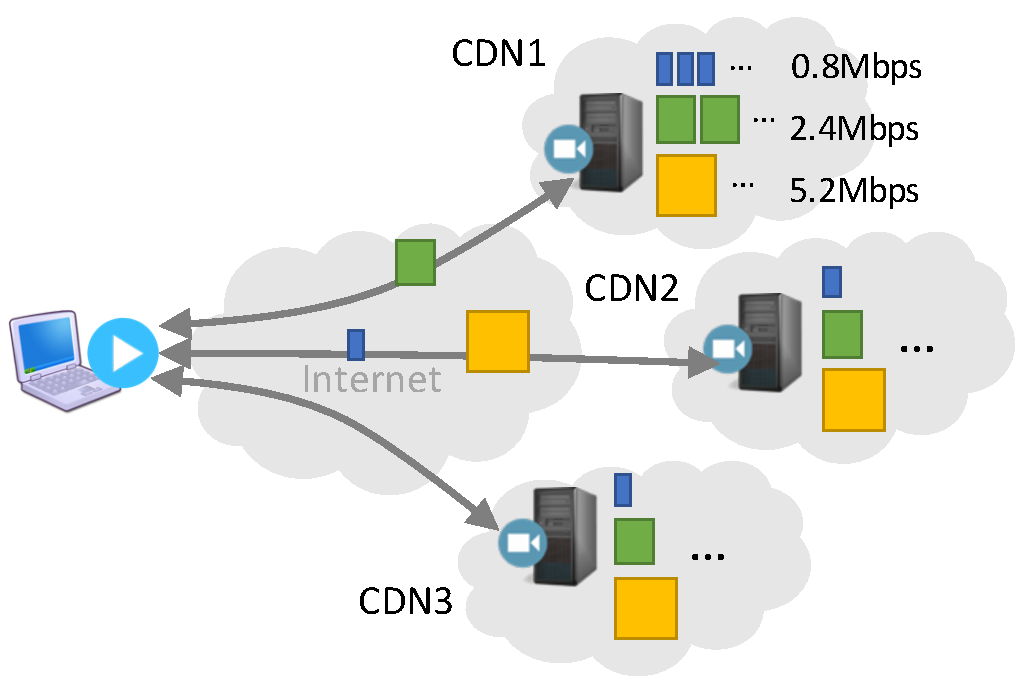
\includegraphics[width=0.5\textwidth] {figures/arch-video.pdf}
   \label{fig:arch:video}
 }
% \hspace{0.4cm}
\subfloat[Internet telephony]{
   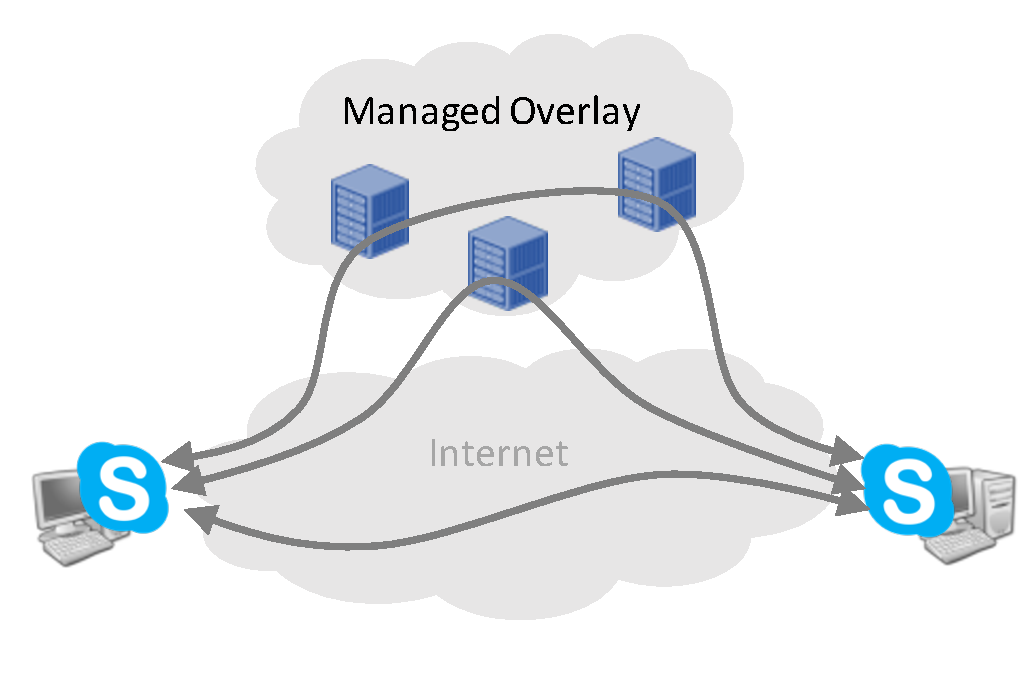
\includegraphics[width=0.5\textwidth] {figures/arch-voip.pdf}
   \label{fig:arch:voip}
 }
\caption{Today's architecture of Internet video and Internet telephony. 
Components relevant to this dissertation are highlighted; other details 
are omitted for clarity. 
The figures depict the configurations (``control knobs'')
that can be adaptively tune on a per-session/-call base in order to improve
QoE.}
\label{fig:app-arch}
\end{figure*}



%\mypara{Advantages of HTTP-based adaptive protocols} 
Compared with connection-oriented protocols, HTTP-based adaptive streaming 
protocols enjoy several advantages~\cite{festive}.
(1) The reliance on HTTP provides more ubiquitous reach and support 
as this traffic can seamlessly traverse enterprise and home
NATs and firewalls~\cite{httpwaist}.
(2)  The video servers are web servers and caches widely available from commercial
CDNs with significantly lower cost than streaming content from dedicated 
servers that support the early-generation connection-oriented video protocols.
(3) Finally, the use of HTTP as the underlying transport protocols allows 
video streaming to benefit from many techniques proposed recently to enhance
web performance and security (e.g.,~\cite{wang2014speedy}).
These practical and performance benefits have been a key driver for rapid 
growth of HTTP-based adaptive streaming protocols.



\subsection{Internet Telephony}
\label{subsec:related:back:voip}

Like Internet video, Internet telephony (or audio-video conferencing services) 
has evolved for more than a decade.
The early architecture of Internet telephony relied on peer-to-peer (P2P)
overlay systems. This key technology, called UDP hole punching, uses 
well-connected peer-to-peer users with public IP addresses 
as {\em supernodes} to enable connections between clients 
who did not have public IP addresses or were behind firewall. 
This technology led to the early success and a dramatic growth of VoIP 
services.

%\mypara{Managed overlays}
Over the past decade, VoIP services such as Skype and Google Hangouts, 
have been evolving from the traditional P2P-based overlay towards 
using {\em managed overlays} which leverage well-connected and well-provisioned 
cloud servers. 
A case in point is Skype, which started off with a peer-to-peer approach to NAT 
and firewall traversal~\cite{Skype-GI08}. 
In the recent years, Skype has adopted managed 
overlay~\cite{VideoTelephony-IMC12}, with some supernodes hosted in the 
cloud~\cite{Skype-Zdnet13}. 
It has been reported that Google Hangouts uses relays in the cloud for all 
calls, and moreover also has streams traverse the cloud backbone from one 
relay to another~\cite{VideoTelephony-IMC12}. 
Figure~\ref{fig:arch:voip} depicts a (simplified) architecture of how 
Internet telephony work over an managed overlay network.
Each call can take either the default path through the public Internet or
a {\em relayed path} that routes the traffic through
one or more relay nodes in the data centers. Relayed paths could include
a single relay to ``bounce off'' traffic or a pair of relays
to enable traffic to ``transit through'' the private backbone of
the managed overlay network.

%\mypara{Advantages of managed overlays}
While both generations of Internet telephony technologies are based on
the same technology of UDP hole punching for NAT and firewall traversal, 
the managed overlay approach enjoys several practical benefits.
(1) Global-scale managed overlays use the cloud infrastructure
which already exists and need not be built up from scratch, while 
P2P overlays involved building up overlay networks from
scratch, which limited their scale.
%, both in terms of physical infrastructure and network
%probing, which limited their scale.
(2) Supernodes in managed overlays are cloud servers
that have high available bandwidth and low latency to edge clients, 
while in P2P overlays, supernodes were regular clients, 
and they sometimes became performance 
bottlenecks due to their limited last-mile bandwidth or computational capacity.
(3) In managed overlays, communications between supernodes are
through well-provisioned private backbone networks, while in P2P overlays, all 
communications must compete bandwidth resources of public networks with
other traffic.


\subsection{Room for Improving QoE}
\label{subsec:related:back:room}

While Internet video and Internet telephony services have been 
evolving towards protocols that have less tunable knobs
(e.g., the HTTP-based streaming protocol cannot 
change bitrate arbitrarily as in traditional protocols, and 
managed overlays provide less overlay choices than 
P2P-based ones)  for practical considerations, 
these protocols still offer enough flexibility and recent research has
shown a substantial room for improving QoE by optimally selecting 
the best configuration for each application session.
%necessarily diminish the room for 
%improving QoE.
%Prior research has shown that these protocols still provide a rich set of control 
%interfaces, and there is a substantial room for improving
%QoE by selecting the right configuration for each
%session.

\begin{itemize}

\item{\em Internet video:} 
Prior research has shown that video QoE can be significantly improved
by better CDN and bitrate configuration for
each video session.
For instance, Figure~\ref{fig:back-cross-cdn} shows that there is 
significant spatial diversity and temporal dynamics of CDN 
performance~\cite{sigcomm12}.
Note that most video players today start with a statically configured 
CDN or a random CDN. This suggests a 
great opportunity of cross-CDN optimization, e.g.,
video buffering ratio can be significantly reduced by dynamically
picking the best CDN for each location and at any point of time.

\item{\em Internet telephony:}
Similarly, it has also been shown that the number of Skype 
calls whose QoE is negatively affected by network performance
can be reduced by over 50\% by judiciously selecting supernodes
to form a relay path for each Skype call~\cite{via}.
(We will elaborate on this in Section~\ref{sec:via:potential}.)


\end{itemize}

\begin{figure*}[t]
\centering
\captionsetup[subfigure]{justification=centering,farskip=-1pt,captionskip=5pt}
\subfloat[Spatial diversity]{
   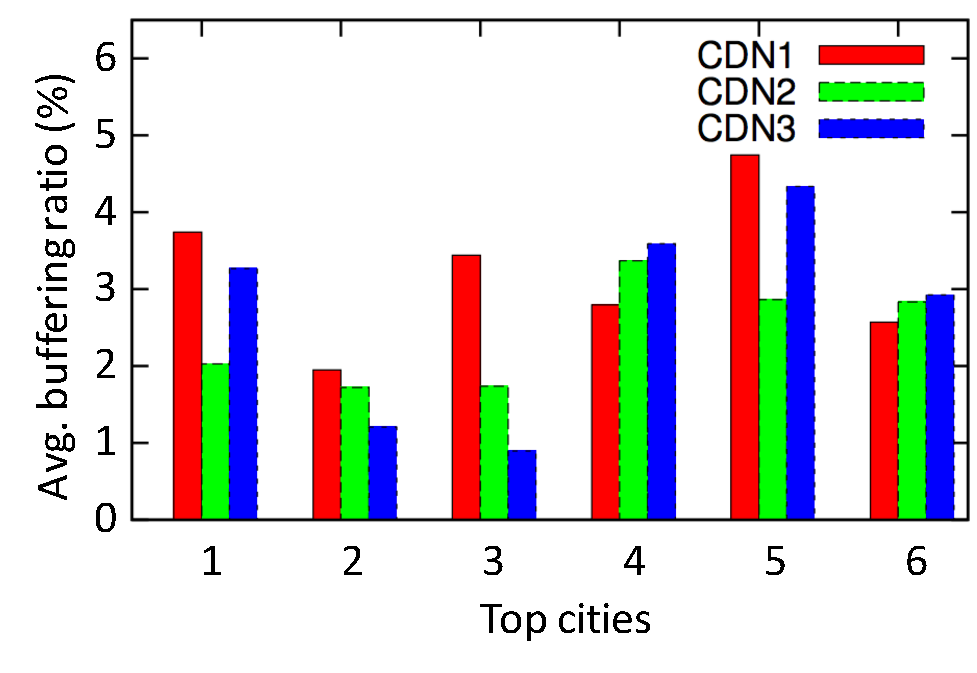
\includegraphics[width=0.4\textwidth] {figures/back-cross-cdn-spatial.pdf}
   \label{fig:back-cross-cdn-spatial}
 }
% \hspace{0.4cm}
\subfloat[Temporal dynamics]{
   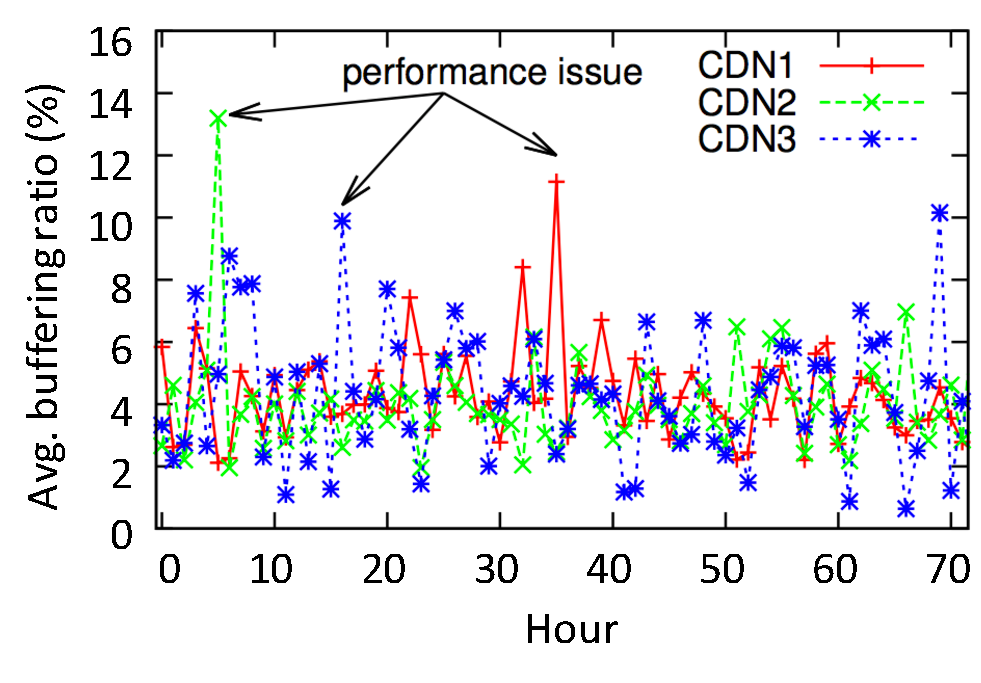
\includegraphics[width=0.4\textwidth] {figures/back-cross-cdn-temporal.pdf}
   \label{fig:back-cross-cdn-temporal}
 }
\caption{Spatial diversity and temporal dynamics of CDN 
performance~\cite{sigcomm12}. 
The figures suggest the opportunity of cross-CDN optimization:
video buffering ratio can be significantly reduced by dynamically
picking the best CDN for each location and at any point of time.}
\label{fig:back-cross-cdn}
\end{figure*}


These measurement results suggest that application QoE is 
sensitive to these configurations, and by customizing for 
each application session with the optimal parameters, 
we can substantially improve QoE over default or static 
configurations which are commonly found in today's 
implementations.


\section{Prior Work on Quality Optimization}
\label{sec:related:quality}

The evolution of the Internet has been driven largely by the need for better 
quality of a variety of applications.
%While Internet applications have always been one of the driving 
%forces behind the evolution of the Internet, 
Around early 2000s, many application providers of video streaming, 
VoIP, and web services started discovering monetization strategies, allowing 
them to scale with reduced costs. 
Since this inflection point, Internet applications have been 
growing and proliferating at an unprecedented pace.
%Especially, over the past decade, we have witnessed a drastic growth and 
%proliferation of Internet applications. 
%The inflection point occurred around early 2000s, when many application 
%providers started discovering monetization strategies for web services, 
%Internet videos, Internet telephony, and etc, allowing them 
%to scale with reduced costs.
%Today, these applications dominate the Internet traffic 
%(video traffic was 70\% of all consumer Internet traffic in 
%2015~\cite{cisco-forecast-2015}) and 
%have become indispensable for daily life
%(Skype users spend over 2 billion minutes 
%talking to each other every day~\cite{skype-2-billion-minutes}).
Not surprisingly, given the importance of Internet applications, understanding 
and improving their quality have a long history of intense research.
%Take video streaming as an example. 
%Early work in 1990s focused on providing QoS in the network, 
%and then focuses have shifted in early 2000s towards more edge-based
%and overlay-based solutions. In recent years, there is a trend to
%revisit the core-network approach enabled the emergence of 
%software-defined networks.
This section introduces a taxonomy of these prior efforts that emphasizes on 
on their inherent trade-offs.
%In Chapter~\ref{ch:overview}, we will use the taxonomy to emphasize the 
%contrast between this dissertation and prior approaches.

Before introducing the taxonomy, I would like to clarify that we use
the term ``Internet quality'' to include both quality of service (QoS) and 
quality of experience (QoE).
While QoS is different to QoE, it is closely relevant to this dissertation 
for two reasons.
First, QoS has a strong (albeit non-linear) correlation with QoE.
For instance, video buffering highly depends on packet loss, and 
VoIP call experience is very sensitive to network latency.
Second, though ultimately we care about QoE, 
much influential work has focused on providing 
QoS in the IP and transport layers.
Readers may refer to, for example~\cite{chen2015qos}, for more 
discussions on the relationship between QoS and QoE.
%can be found towards the end of this section.

\mypara{Taxonomy} 
The prior approaches to quality optimization can be categorized
based on their answers to a key architectural question: {\em where should the
functionality of quality optimization be implemented?}
There are two dimensions in the answers to the questions:
\begin{itemize}

\item {\em Where in the network?} 
There are two natural options: 
{\em endpoint-based} solutions which rely only on endpoints (e.g., clients, 
servers, caches), and 
{\em in-network} solutions which require assists from in-network devices 
(e.g., switches, routers).
To avoid any ambiguity, solutions that involve both endpoints and in-network 
devices (e.g., router-assist congestion control) fall into in-network solutions
under such dichotomy,
because they share similar advantages and disadvantages with other 
in-network solutions.
Note that although early in-network solutions only operate in or below the IP layer, 
this has since changed as in-network devices move up in the protocol stack to 
provide richer services (e.g., router-assist video 
streaming~\cite{sdndash}).

%There are two natural options: in-network and endpoints. 
%The difference between the two categories used to be straightforward--in-network 
%devices provide functionality below the IP layer for scalability, 
%while endpoints support transport- and application-layer functionality.
%The boundary, however, has become blurred as in-network devices
%move up in the protocol stack to provide richer services (e.g., router-assist video 
%streaming~\cite{bentaleb2016sdndash}).
%That said, we can still categorize prior approaches into:
%{\em endpoint-based} solutions which rely only on endpoints (e.g., clients, 
%servers, caches), and 
%{\em in-network} solutions which require assists from in-network devices 
%(e.g., switches, routers).
%The choice between endpoint-based solutions and in-network ones reflects
%the tradeoff between deployability and performance benefit; 
%while in-network solutions are arguably more difficult to be deployed 
%in practice than endpoint-based solutions, they could potentially achieve 
%better performance by finding better network paths and allocating bandwidth
%more efficiently, both of which are infeasible endpoint-based solutions.

%\item {\em What scope of measurement to drive quality optimization?}
%At one extreme, we have a purely decentralized approach where each 
%device (in-network or endpoint) or flow can improve quality by adapting 
%to network conditions inferred from its {\em locally observed} information.
%At the other extreme, we can imagine a logically centralized approach where
%the adaptation of each device or flow is driven by information from {\em multiple
%viewpoints}; e.g., from other clients of the same content provider.
%The tradeoff between the two extremes is that it may be intrinsically difficult 
%for the decentralized approach to accurately network conditions, while 
%the logically centralized approach poses additional complexity to the system, 
%e.g., gathering data from multiple viewpoints, which needs to be justified by
%improved quality.

\item {\em Which level in the protocol stack?}
Because our ultimate objective is to improve application-level QoE, 
it is natural that the solution should have access to the applications themselves,
i.e., at the application level.
That said, the layering nature of the protocol stack means that any improvement in 
the lower-level protocols (e.g., TCP, routing, wireless adaptation) may benefit the 
application-level quality.
%That said, in choosing the level in the protocol stack, there is a tradeoff between 
%more visibility to QoE and more controllability.
%On one hand, because our ultimate objective is to improve application-level QoE, 
%it is natural that the solution should have access to the applications themselves.
%On the other hand, lower layer solutions operate on a finer timescale 
%(e.g., per-packet) and have access to more feedback from the 
%Internet (e.g., packet loss), which is invisible to applications, which sometimes
%run in a user-space sandbox (e.g., browsers).

\end{itemize}




\begin{figure}[t!]
\centering
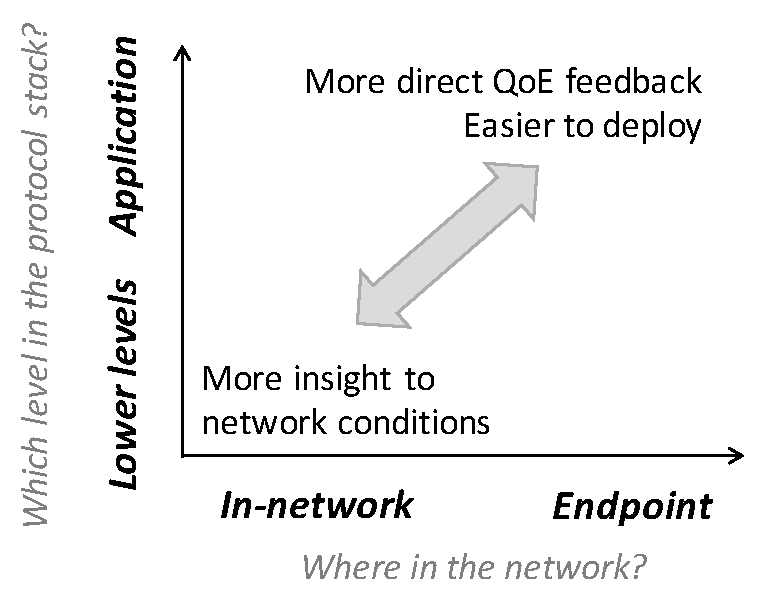
\includegraphics[width=0.5\textwidth]{figures/back-tradeoff.pdf}
%\vspace{-0.3cm}
\caption{Prior approaches can be categorized by their placement of
the functionality of quality optimization along two dimensions.
These design choices must make fundamental trade-offs between 
more visibility to QoE and more visibility to network conditions.}
\label{fig:back-tradeoff}
\end{figure}

\mypara{Design trade-offs}
The choices regarding these two dimensions involves a key architectural 
trade-off, illustrated in Figure~\ref{fig:back-tradeoff}.
\begin{itemize}

\item {\em More visibility to user-perceived QoE:} 
On one hand, optimizing quality at endpoints and the application layer has 
the advantage of more direct and accurate information on user-perceived 
QoE, which usually is available only to client-side applications.
This allows their optimization logic to be driven directly by the QoE as 
feedback. Implementing optimization functionality in endpoints at the 
application layer also carries the practical advantage of more flexibility since 
their software is upgraded more frequently than in-network devices or 
lower layer protocols.

\item {\em More visibility to network conditions:}
On the other hand, while in-network solutions in the lower layers have to rely 
on indirect metrics to infer QoE from encrypted application-level 
communications~\cite{mobicom2014-qos,
aggarwal2014prometheus,imc2012-firstbyte}, 
they enjoy the architectural advantage that they have more accurate and 
finer-grained information on the network conditions (e.g., per-packet congestion 
loss).
%which is opaque to applications typically running in a user-space sandbox 
%(e.g., browsers).
Applications running in user-space sandboxes (e.g., browsers) are often 
oblivious to changes in these low-level network conditions.

\end{itemize}



%Note that while these dimensions seem to dependent (e.g., in-network solutions
%are traditionally believed to operate only in IP layer), as we will 
%see next, they are indeed orthogonal, and there have been (or could be) 
%valid design points given each combination of answers to these questions.

Next, we use the taxonomy to put prior work in perspective.

\subsection{In-Network Solutions}
The in-network approach has long been a focus of intense research. 
In-network solutions can provide better services at multiple layers on
the protocol stack.

%\begin{itemize}
%\item QoS
%\item Router-assist TCP
%\item SDN
%\end{itemize}

\mypara{IP-layer support for QoS}
%As defined by the Internet Engineering Task Force (IETF), 
The two most prominent proposals of QoS services are
the Integrated Services (IntServ) and Differentiated Services (DiffServ). 
IntServ~\cite{intserv} uses the resource
reservation protocol (RSVP)~\cite{rsvp} to provide the
QoS by reserving resources explicitly at all routers along an end-to-end 
path, and hence all routers must keep states related to services,
leading to prohibitive scalability and complexity issues.
In contrast, the DiffServ~\cite{diffserv}
aggregates flows into pre-configured classes based on packet header 
fields, and hence is  more scalable. However, since DiffServ treats 
packets in the same class identically, it is difficult to provide QoS with
strong semantics to individual flows.
Another widely used technique is the Multiprotocol Label Switching 
(MPLS)~\cite{mpls}, which reduces 
the routing complexity and table lookups by packet labeling techniques.
Other in-network schemes also seek to provide richer services by adding
more functionality to IP layer, such as Multicast~\cite{mbone}.
With rapid growth of Internet traffic and applications, 
these early solutions have become increasingly unfit to cope
with the need for QoS with stronger semantics and 
more scalable implementation over 
an increasingly ossified infrastructure.
%The recent rapid growth of Internet traffic and applications 
%has led to the need for a solution that provide stronger QoS semantics in a 
%scalable manner, and over an increasingly ossified infrastructure.
%Hence, the basic approaches such as DiffServ and IntSev seem 
%fundamentally unfit to cope with these trends.
These trends have inspired many new in-network solutions 
over the past decade, including novel QoS service architecture (e.g., 
Core-Stateless Fair Queueing~\cite{csfq}) and clean-slate solutions (e.g.,
Active Networks~\cite{active-network}, Network OS~\cite{nox}, and 
Content-Centric Networks~\cite{ccn}).
While these efforts have enduring impact on the ensuing research,
they impose   significant deployment cost to revamp the existing ISP
infrastructure.
As a result, the Internet today still only provides best-effort
service to most applications.

\mypara{Router-assist congestion control}
While congestion control is an end-to-end functionality, many 
proposals have shown that congestion control may benefit from 
explicit router assistance, such as providing explicit or implicit 
feedback on network congestions 
(e.g., ECN~\cite{ecn},
XCP~\cite{xcp}, RCP~\cite{rcp}, VCP~\cite{vcp}),
and Active Queue management (AQM) schemes (e.g., RED~\cite{red},
AVQ~\cite{avq}, and CoDel~\cite{codel}).
In XCP and RCP, each router along an end-to-end path marks 
special bits on the packet header to help the senders determine the 
end-to-end available bandwidth. 
AQM schemes in contrast aims to prevent persistent queue buildup
in routers, by marking packets with ECN or dropping them before 
the queue is full, such as in~\cite{red}.
Similar to IP-layer support for QoS, 
these methods also add significantly complexity to in-network
devices and thus induce significant deployment cost.
Moreover, most proposals require making changes 
on all ISPs along the end-to-end paths, creating more
barriers to deployment.
A notable exception is in data centers, where 
router-assist congestion control mechanisms are widely used, 
because network devices, and end hosts are under the same 
administrative domain, and are upgraded on a regular basis.


\mypara{SDN-based approach}
SDN is a new network architecture 
to greatly simplify network management~\cite{feamster2014road}
by separating the data plane from the control plane that determines 
the routing states~\cite{OpenFlow}, thus making the data plane 
``programmable''.
The SDN-based solutions have  many open-source offerings
(e.g.,~\cite{onos,floodlightopenflow}), and offer a viable path to
the deployment of new routing 
protocols, as routing table may be updated in near real-time without
interrupting any ongoing traffic~\cite{rexford-sdn-update},
allowing routing to programmable on a per-flow basis.
Moreover, recent research on high-speed SDN-enabled routers has 
suggested that such programmability can be realized on a per-packet level 
to implement AQM schemes  in a scalable 
manner~\cite{sivaraman2016programmable,sivaraman2016packet}.
The logically centralized nature of SDN also offers an opportunity
that individual ISPs can coordinate with other ISPs
(e.g.,~\cite{schapira2010putting}) to provide end-to-end optimization
and even application QoE optimization (e.g.,~\cite{sdndash}).
%While SDN has the potential to bring ISPs into the loop of QoE optimization,
In today's federated Internet architecture, optimizing 
end-to-end quality requires multiple ISPs to coordinate, but 
even if each ISP is willing to adopt SDN paradigm for reducing management costs,
it remains unclear whether they have the incentives to coordinate
to optimize end-to-end application quality.

\subsection{Endpoint Solutions}
In contrast, the endpoint-based approach relies on endpoints to adapt to changes
in network conditions and resource availability.

\mypara{Overlay routing}
Overlay networking has been proposed as an alternative to adding functionality 
to the network core. It has been applied in a variety of contexts, such as 
virtual private networks (VPNs) and multicast~\cite{esm,ALMI-USITS01,
Multicast-Sigcomm02}. 
Of interest to us here is work focused on overlay routing with a view to improving 
routing QoS and robustness~\cite{Detour-Sigcomm99,RON-SOSP01}. 
This work showed that network performance such as 
delay, packet loss, and reliability, could be improved by using 
an overlay path that traverses well-chosen waypoints. 
Despite this promise,  overlay routing for performance gains has not seen 
much adoption in practice, for several reasons including the last-mile 
performance bottlenecks when client nodes are used as as peers, and 
the policy issues involved in turning stub networks (e.g., university campus 
networks) into de facto transit networks. 
Perhaps most importantly, these early systems operate on a relatively 
small scale (e.g., RON~\cite{RON-SOSP01} 
had tens of machines), and hence they still lack 
enough information to maintain an up-to-date view of the dynamic network 
conditions. It is also unclear whether these systems
can scale up to support today's applications running on millions of 
clients.
%involved building up overlay networks from scratch, both in terms 
%of physical infrastructure and network probing, which limited their scale.

%\mypara{CDN}


\mypara{Congestion control}
Over the past decades, TCP congestion control has received intense 
research in the literature; from the early efforts towards a 
general-purpose scheme 
(e.g.,~\cite{jacobson1988congestion,brakmo1994tcp,tcp-compound})
to later work on specializing congestion control in different operational
environments (e.g., data center~\cite{alizadeh2010data},
high bandwidth-delay product networks~\cite{cubic}, and satellite 
connections~\cite{tcp-hybla})
and to the latest efforts towards a unifying scheme by using 
machine-generated code~\cite{remy} and modeling networks 
as a blackbox~\cite{pcc}.
Current congestion control schemes suffer from a key
limitation that they only {\em react} based on the locally observed
information; e.g., without assistance of routers, they will only
react after congestion has caused packet loss or latency inflation.
A notably exception is congestion 
manager~\cite{balakrishnan1999integrated,spand},
which aggregates information of multiple TCP connections to 
predict network performance for a new connection, but these
schemes involve changing the kernel or setting up management 
server, and thus did not see wide adoption.
Moreover, state-of-the-art congestion control schemes may 
mismatch with the goal of applications~\cite{usenix12_ghobadi},
and even cause bad interaction with control loops in 
the application layer~\cite{confused,festive}, indicating that
application-layer adaptation might be in a better position to meet
the need of applications.

\mypara{Application-level adaptation}
To cope with the dynamic network conditions, 
most applications run custom client-side adaptation logics in
the application layer, rather than relying on transport-level or 
in-network solutions for two reasons:
(1) clients is in the best position to detect and respond to 
QoE problems; and 
(2) recent work suggests the need for cross-CDN 
optimizations~\cite{sigcomm12} and 
flexible web object scheduling~\cite{butkiewicz2015klotski},
which implies the need for keeping minimal state in the
network or servers.
In video streaming, most commercial products 
today perform proprietary client-side bitrate adaptation 
(e.g.,~\cite{SmoothStreaming,akamaihd,hls,netflix}) 
over HTTP-based adaptive streaming 
protocol~\cite{dash}.
Many studies have identified problems in existing
client-adaptation algorithms 
(e.g.,~\cite{mmsys2011cisco,de2010experimental}),
bad interactions with TCP control loops
(e.g.,~\cite{confused,usenix12_ghobadi}),
and techniques to improve bitrate adaptation 
(e.g.,~\cite{nossdav12_akhshabi,festive,panda}). 
Other efforts have demonstrated inefficiencies in existing 
CDN and server selection
strategies~\cite{youtubecdn,youtube-infra,sigcomm12,sigcomm12cdnmulti}.
%Many studies have shown the limitations of these 
%solutions~\cite{confused,mmsys2011cisco} and 
%proposed endpoint solutions to fix them~\cite{festive,panda}.
In Internet telephony, there has been work to improve 
client-side rate adaptation through multi-path wireless~\cite{diversifi},
network performance profiling~\cite{sprout,de2008skype}, and 
better supernode selection~\cite{baset2004analysis,Skype-GI08}).
A shared feature of these schemes is that the adaptation is driven by
local information observed by a single application session.
A notably exception is SPAND~\cite{spand}, which proposed to improve 
endpoint adaptation by sharing passive measurement from multiple 
endpoints  at the application layer.
This dissertation is in part inspired by SPAND and revisits
its ideas in the light of the advances in large-scale data analytics
and pervasive client-side instrumentations in today's Internet 
applications.


\mypara{Network performance prediction}
The key issue of endpoint adaptation is that it can only rely 
on limited, locally observed information to {\em react} to
changes in network conditions.
To overcome this limitation, many studies have attempted to 
predicting network performance, such as latency and
available bandwidth, by exploiting
stability and stationarity of network performance
(e.g.,~\cite{hu2005measurement}), constancy of various network
metrics~\cite{zhang2001constancy,balakrishnan1997analyzing}, 
and longitudinal patterns of cellular
performance (e.g.,~\cite{nikravesh2014mobile}).
%
%Moreover, measurement studies on path properties have 
%show certain stability and predictability of network performance;
%they have shown prevalence and persistence of network bottlenecks
%(e.g.,~\cite{hu2005measurement}), constancy of various network
%metrics~\cite{zhang2001constancy,balakrishnan1997analyzing}, 
%and longitudinal patterns of cellular
%performance (e.g.,~\cite{nikravesh2014mobile}).
%Inspired by these measurement studies, 
Researchers have explored three approaches to network performance prediction:
(1) to use  packet-level probes to
estimate end-to-end performance 
(e.g.,~\cite{prasad2003bandwidth,
hu2004locating, strauss2003measurement, jain2003end}),
(2) to build an ``Internet performance map''
based on active probes from a selective set of 
``vantage points'' (e.g.,~\cite{iplaneosdi, spand,ramasubramanian2009treeness,
dabek2004vivaldi}), and 
(3) to leverage the
history of the  same client-server pair 
(e.g.,~\cite{vazhkudai2001predicting,
jain2005end, swany2002multivariate,
mirza2007machine, he2005predictability}).
While this work has shown substantial benefit of accurate performance
predictions, it has not seen wide adoption for practical 
reasons: the packet-level probing requires 
per-packet information which is invisible to applications,
the Internet-map approach needs a dedicated 
monitoring infrastructure, and the history-based approach requires
enough history be accumulated before performance prediction is 
feasible, but many application sessions, such as web, 
consist of a few short-lived flows sent from different servers.



%Prior measurement studies on path properties have shown
%prevalence and persistence of network bottlenecks
%(e.g.,~\cite{hu2005measurement}), constancy of various network
%metrics~\cite{zhang2001constancy}, longitudinal patterns of cellular
%performance (e.g.,~\cite{nikravesh2014mobile}), and spatial similarity of
%network performance (e.g.,~\cite{balakrishnan1997analyzing}),
%which suggest that throughput can be predicted with reasonable 
%accuracy.



% This includes the work on  identifying
%problems \sh{existing} in client-adaptation algorithms
%(e.g.,~\cite{mmsys2011cisco}), interactions with TCP control loops
%(e.g.,~\cite{usenix12_ghobadi,nossdav12_esteban}), and techniques to improve 
%bitrate adaptation (e.g.,~\cite{nossdav12_akhshabi,festive}).  Other efforts
%have demonstrated inefficiencies in CDN and server selection
%strategies~\cite{youtubecdn,youtube-infra}.  Recent work has suggested
%cross-CDN optimizations to improve video
%quality~\cite{sigcomm12,sigcomm12cdnmulti}.


%\begin{itemize}
%\item Overlay routing
%\item CDN
%\item TCP
%\item DASH
%\end{itemize}



\subsection{Other Related Work}

Finally, we discuss other directions closely related to this dissertation.

%\begin{itemize}
%\item  QoE vs. QoS
%\item Quality measurement
%\item video related research
%\end{itemize}

\mypara{QoE metrics}
A key aspect in  video  and VoIP delivery is the need to
optimize user-perceived  QoE. While there is evidence that
video viewers are sensitive to frequent bitrate switches 
(e.g.,~\cite{user-adaptive}), sudden
changes in bitrate (e.g.,~\cite{videoqoe}), and  buffering (e.g.,
\cite{sigcomm11}), it is somewhat surprisingly challenging 
to design a good QoE metric (e.g.,
\cite{qscore}), and this is still an active area of research.
While recent work also suggests ISPs are inferring  user 
experience from network-layer measurements and QoS metrics 
(e.g.,~\cite{mobicom2014-qos,sigmetrics2014-correlation,
aggarwal2014prometheus,
imc2012-firstbyte,sigcomm2010-mercury}), we argue that 
application providers are in a better position than these 
infrastructure providers to measure and adapt to QoE.
The goal of this dissertation is not to offer new QoE models, 
but to improve  the metrics that are known to have high impact 
on user experience.

\mypara{Video measurements}
There are many recent measurement studies on
understanding video content popularity and access patterns
(e.g.,~\cite{youtube-imc07}\cite{plissonneau2012longitudinal}), 
flash crowds during highly popular events (e.g.,~\cite{beijing-imc09}), 
and their implications for CDN and caching designs.  
While these efforts help motive the techniques proposed in 
this dissertation, our goal again is to understand the structure of 
quality problems and further develop solutions to actually improve
QoE.

\vspace{0.5cm}
While both in-network solutions and endpoint solutions have 
to compromise on either visibility to QoE or visibility to network conditions,
the solutions proposed in this dissertation 
strikes a better balance by taking advantage of the access of millions of 
endpoints with a data-driven approach.
%enabling an endpoint-based data-driven approach.


\section{Prior Work on Data-Driven Optimization in Networking}
\label{sec:related:data}

Another direction closely related to this 
dissertation is the application of the data-driven paradigm to improving 
networked systems. 
We introduce a taxonomy of how networked systems can benefit from the 
data-driven paradigm.
We also use a concrete case study to show how data-driven ideas can
be applied to improve TCP congestion control in different ways. 

While most systems already use data-driven techniques 
(e.g., TCP congestion control schemes react against congestion 
signals such as packet loss and round-trip time),
we argue that they could be substantially
improved by borrowing systematic frameworks from data science
literature and further exploring more data-driven opportunities by
leveraging more available data.
In particular, we observe two aspects of network systems along 
which the data-driven paradigm can help:
{\em better setting of parameters} within the existing adaptation logic,
and {\em better run-time decision making logic} to replace the existing one.

Since the way in which networking problems benefit from data-driven 
techniques bears much resemblance to 
other systems areas, 
this section will focus on networking problem, but also draw 
related work from a broad set of systems areas.

\subsection{Type I: Better Settings of Parameters}

The conventional wisdom has been that in most of network protocols, 
the adaptation should use {\em hand-picked} parameters, (e.g., TCP parameters 
such as initial congestion window size and AIMD parameters).
Recent research, however, has shown that performance
can be improved by {\em automatically} tweaking these parameters 
to achieve better performance in different operating conditions
(e.g., better parameters of TCP congestion control~\cite{remy,googleinitwindow}, 
AQM logic~\cite{shah2016sam,lin2015kemy}), configurations of routing algorithms 
(e.g.,~\cite{sharma2017machine}, and workload modeling in wireless 
networks~\cite{alsheikh2014machine}).
Recent research has also shown similar data-driven opportunities 
in other areas including CPU cache replacement policy~\cite{calvinlin-cache},
database consistency management~\cite{aaron-cidr}, and 
rational database system management~\cite{andypavlo-rbsm}.
While these efforts are in entirely different areas, they have largely 
exploited the same inefficacy in traditional
control logic that the parameters are statically configured 
based on assumptions that are ill-matched with the dynamic workload 
in runtime.  
Such problem can be fixed by dynamically training
these parameters with recent measurements
(e.g.,~\cite{calvinlin-cache}) or synthetically simulated data (e.g.,~\cite{remy}).
The problem of learning the best configurations
for a complex system is conceptually similar to the 
hyper-parameter selection problem in machine learning~\cite{ml101}.

\noindent\underline{\smash{Case study: Tunning congestion control parameters:}}
We use TCP congestion control as a case study to show
how a protocol can be improved by tuning the key parameters.
%In Remy~\cite{remy}, if we want to optimize for a given 
%performance metric (e.g., flow completion time) under 
%some given network characteristics 
%(e.g., mean round-trip time and packet loss rate), Remy 
%can train key congestion control parameters such as 
%AIMD parameters and the timeout threshold using offline
%simulation against traffic synthetically generated based on
%the given network characteristics.
Prior work on Remy~\cite{remy} showed that a machine-designed 
TCP that uses offline simulation driven by prior  knowledge of the 
network context (e.g., topology, degree of multiplexing) can learn 
the best values of some key constants and achieve significant 
performance improvement over today's manually picked values; 
e.g., a simulated 15 Mbps fixed-rate link with eight senders 
contending and an RTT of 150 ms, Remy-generated control logic achieves 
40+\% throughput speed up and 20+\% delay reduction over many 
specially engineered TCP variants.


%\begin{itemize}
%\item TCP
%\item Cache replacement
%\item database configurations
%\end{itemize}

\subsection{Type II: Better Run-Time Decisions}

While finding better parameters of the existing control logics
can improve performance, it is arguably incomplete, since it still uses 
handcrafted control logics based on analytical model that models the 
relationship between the feedback signals (e.g., RTT) with internal states of the 
underlying system (e.g., router queue occupancy). 
While this approach served us well for decades, it is fundamentally inefficient 
to characterize today's application delivery systems, which have grown too 
complex to model analytically. Rather than merely tuning the parameters for 
the existing control logic, recent research has made a case for a 
more direct approach in which the logic models the network as a 
blackbox and use measurement data to drive the decision making.
In other word, rather than inferring the underlying network states and finding
best decisions analytically, it builds a model that directly associate quality
feedback with decisions (configurations).
Research has shown that this more direct data-driven 
approach can improve the performance of routing~\cite{schapira2010putting},
TCP throughput~\cite{pcc}, server selection in web 
performance~\cite{footprint}, as well as bitrate adaptation in 
video streaming~\cite{neural-streaming}.
Besides networking problems, this approach also found its
application in improving resource scheduling in 
cloud services~\cite{cherrypick}.
%The basic idea of this type of data-driven approach is
%build a blackbox model to describe the relationship between 
%action (decisions) and performance feedback, 
The techniques commonly used in these solutions are largely based on 
exploration-exploitation strategies (multi-armed techniques~\cite{mab}), or 
Bayesian optimization~\cite{bayesian-optimization}), in which feedback of 
network performance is used to explore the decision spaces.
Compared to the first type, the main advantage of the 
second type is that it could converge to a better decision
faster by making minimal assumption about the 
underlying  systems. 
A primary drawback, however, is that it has less interpretability
as the underlying system is modeled as a blackbox.


\noindent\underline{\smash{Case study: Blackbox-based congestion control:}}
Again, we use TCP congestion control as a case study to show
how a protocol can be transformed to a simpler logic driven
completely by measurement data, while making less
assumptions on the underlying network system.
PCC~\cite{pcc} attempts to simplified TCP congestion 
control algorithm by using locally observed performance 
to directly drive the setting of congestion window size. 
Specifically, it continuously maintains a model between 
observed performance (e.g., throughput and latency) 
and cwnd. This approach greatly simplifies TCP congestion
control, while at the same time, significantly 
improves TCP performance; e.g., 10$\times$ higher
throughput of TCP CUBIC on global commercial Internet.

%\begin{itemize}
%\item video streaming
%\item pcc
%\item routing
%\end{itemize}

%The boundary could be blurred

%mention KnowledgePlane

%\subsection{Discussion}
%
%There are three final remarks regarding the the various ways the 
%data-driven paradigm is applied in networking research:
%
%%\mypara{Data-driven and ML-based diagnosis} 
%First, while we focus on using data-driven technique for 
%better adaptation, many efforts have shown similar data-driven 
%opportunities in better diagnosis of complex network systems~\cite{knowledgeplane,attmanagement}.
%
%%\mypara{} 
%Second, the boundary between these two types of data-driven 
%approaches is in fact not as clear as we discussed. 
%
%Finally, while the Type II approach uses more real-time data
%to directly drive the adaptation, it only leverages the same
%data available to other prior work. In endpoint solutions,
%it would be fundamentally limited by the scale and scope 
%of the locally measurable data.


\section{Summary}

In the first part of this chapter, we have used empirical studies 
to show that QoE problems are pervasive in Internet video and Internet 
telephony. Then we have introduced related background on today's 
Internet video and Internet telephony services.

In the second part of this chapter, we have introduced a taxonomy
to highlight the inherent trade-offs in prior work to improve Internet 
application quality. %--in-network solutions and endpoint solutions.
%In particular, we have focused on the architectural trade-offs
%in their placement of the functionality of quality optimization.
In-network solutions have more direct and accurate visibility to 
network conditions, while endpoint solutions can measure metrics
more directly related to user-perceived QoE, and are  usually more deployable.
%While prior work has to compromise on at least one front,
As we will see, our solution strikes a better balance
between the visibility to user-perceived QoE and the visibility to 
network conditions through taking a more data-driven approach to 
endpoint solutions.

In the last section, we have discussed two approaches to using the
data-driven paradigm to improve network systems: improving setting
of parameters, and improving real-time decision-making logic.
While our solution follows the second type, it unleashes more 
data-driven benefit by taking advantage of more data of real-time 
measurements collected from millions of endpoints.







\chapter{Overview}
\label{ch:overview}

The main contribution of this dissertation is to provide {\em a suite of solutions
that make data-driven QoE optimization practical}.
In particular, we  demonstrate that one can achieve substantial QoE improvement
by utilizing measurement data already available to today's application 
providers and integrating domain-specific insights with machine learning 
techniques to make better real-time adaptation for client-side applications.
%In this chapter, we give an overview of our solutions, the key insight
%behind our solutions, and a perspective of how this solution compared 
%to prior efforts of Internet quality optimization and applying data-driven
%in the networking literature.

This chapter is organized as follows.
Section~\ref{sec:overview:arch} gives an overview of the envisioned 
architecture of data-driven QoE optimization, 
called {\em Data-Driven Networking} or {\em \ddn}.
%some illustrative examples of how different applications 
%may benefit from \ddn, and perspective of how this solution compared 
%to prior work.
Section~\ref{sec:overview:challenges} discusses the key technical 
challenges for \ddn to achieve non-trivial QoE improvement.
Section~\ref{sec:overview:unifying} presents the key insight,
and Section~\ref{sec:overview:solutions} 
describes a suite of solutions inspired by the insight to address \ddn's
challenges in the context of Internet video and Internet telephony.


\section{Formalizing \ddn}
\label{sec:overview:arch}

In this section, we present a conceptual overview of the Data-Driven 
Networking (\ddn) paradigm (Section~\ref{subsec:overview:concept}),
and some illustrative examples of how different applications   
may benefit from \ddn (Section~\ref{subsec:overview:examples}).
We end this section by contrasting it to prior
approaches (Section~\ref{subsec:overview:contrast}).
%We end this section by identifying key factors that can impact 
%the potential benefits of \ddn.

\subsection{Conceptual Architecture}
\label{subsec:overview:concept}

\ddn is a new paradigm for designing the adaptation logic of 
end-to-end protocols. 
Unlike prior endpoint approaches, 
\ddn-based control loop is driven by real-time
{\em multi-session} (not single-session) view of 
{\em in-situ quality}~\cite{insitu} 
measurement (not active
measurements or indirect metrics), 
and {\em automatically tuned actuation algorithms} based
on data-driven insights (with little to no manual tuning).

The workflow of \ddn consists of two components:
(a) the {\em client-side instrumentation} integrates with the 
client-side application%\footnote{We use ``client'' to denote where a session is actually run.} 
to measure per-session client-perceived quality and apply 
decisions made by \ddn; and (b) the {\em \ddn controller} 
runs two loosely coupled steps:
\begin{enumerate}
\item Aggregate quality measurement from client-side 
instrumentation into {\em multi-session view} -- 
some actionable insight which summarizes the performance of
sessions with similar QoE-determining factors.
\item Make control decisions based on the multi-session 
views, and send them to client-side instrumentation for execution.
\end{enumerate}

Note that the \ddn paradigm is compatible to 
the existing infrastructure operated by many application 
providers. For instance, many application providers 
have already deployed client-side instrumentation to
monitor client-side information in real-time and collect
measurement for offline analytics (e.g.,~\cite{sigcomm11}).
Many application providers also maintain a global control
platforms (e.g.,~\cite{c3,via,footprint,chen2015end}) 
where the \ddn controller can be implemented.


\begin{figure}[t!]
\centering
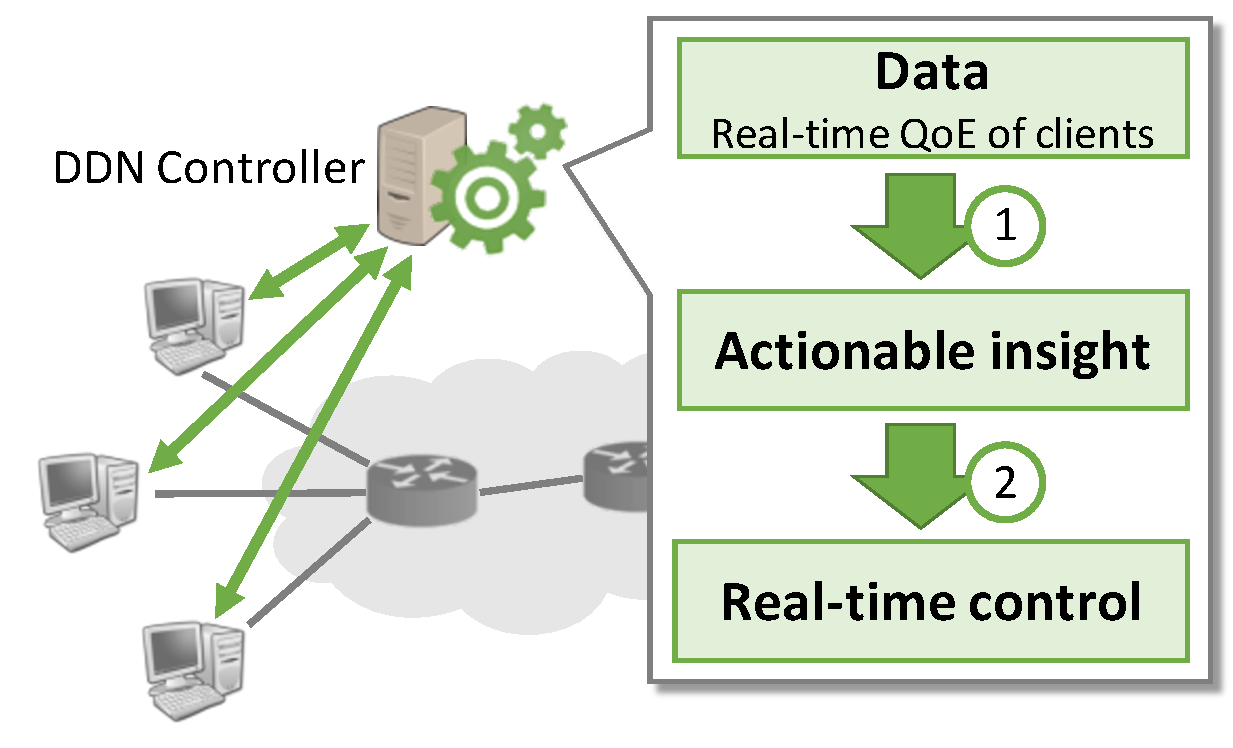
\includegraphics[width=0.6\textwidth]{figures/overview-ddn-arch.pdf}
%\vspace{-0.3cm}
\caption{Overview of the \ddn controller}
\label{fig:intro-contribution}
\end{figure}

\subsection{Contrast to Prior Work}
\label{subsec:overview:contrast}

\subsubsection{Compared to Prior Work on Quality Optimization}

In Section~\ref{sec:related:quality}, we have classified
prior work on quality optimization along two dimensions:
where in the network (in-network vs. endpoints), and
which level in the protocol stack (application vs. lower layers).
Using this taxonomy, \ddn should be classified as an 
endpoint solution operating in the application layer.


Compared to prior application-level endpoint solutions,
decision making of \ddn is driven by information of multiple sessions, 
rather than single session. 
The core argument of \ddn is that {\em it is feasible to
maintain an accurate view of network conditions based on the QoE information
collected from many endpoints}.
%Traditional end-to-end adaptation protocols (e.g., TCP/DASH) 
%is driven by what is observed by a single session. In contrast, 
By extending the spatial scope of QoE measurement, 
\ddn can predict the quality of a session if it uses certain decision, 
as long as the decision has been used by 
some similar sessions.
\ddn is in part inspired by seminal work such as SPAND~\cite{spand},
and our contribution lies in providing end-to-end solutions to make \ddn
practical in today's applications, by leveraging the recent advances
in large-scale data analytics and domain-specific insights.
In short, \ddn retains the ethos of the endpoint approach, 
while addressing its lack of
visibility to network condition by leveraging an expended view 
across many endpoints.

Compared to in-network solutions or endpoint solutions operating 
in lower layers, \ddn enjoys the advantage that it has  
direct access to in-situ quality measurement.
In \ddn, what to be ``sensed'' is exactly what to be optimized, 
i.e., quality perceived by all historical and ongoing sessions; 
not indirect signals on quality (e.g., acks 
or bandwidth), or active probes from a handful 
of vantage points (e.g., iPlane~\cite{iplaneosdi}). 
While in-situ quality data may compromise on the fidelity of 
individual measurement, they are far more efficient than 
alternatives in obtaining a panoramic and representative
 view of client-perceived quality from growingly diverse platforms~\cite{insitu}.
%and the lack of fidelity can be compensated by harnessing the ``unreasonable effectiveness of data''~\cite{google-data}.
Relying solely on in-situ quality data also serves pragmatic 
purposes as many application providers today already have 
a vested interest in measuring user-perceived quality for 
various reasons~\cite{sigcomm-qoe-workshop}.







%To understand the contrast between  \ddn and traditional 
%control planes, it is useful to revisit the two logical steps 
%in the workflow of {\em any} control plane 
%(Figure~\ref{fig:sensing-actuation}):
%{\em sensing}, which gives the feedback data to control plane, 
%and {\em actuation}, which turns the feedback data to control decisions.
%\ddn radically departs from non-\ddn designs on both fronts 
%with two definitive features.

%(Table~\ref{tab:ddn} provides some examples to contrast between \ddn and non-\ddn designs.)

%\begin{itemize}
%\item {\em Multi-session view:} 
%Sensing of \ddn is based on multiple sessions, rather than single session. 
%Traditional end-to-end adaptation protocols (e.g., TCP/DASH) 
%is driven by what is observed by a single session. In contrast, 
%By extending the spatial scope of sensing to many sessions, 
%\ddn can predict the quality of a decision even before a session 
%actually uses it, as long as the decision has been used by 
%some similar sessions.
%
%\item {\em In-situ quality:}
%In \ddn, what to be ``sensed'' is exactly what to be optimized, i.e., quality perceived by all historical and ongoing sessions; 
%not indirect signals on quality (e.g., acks~\cite{jacobson1988congestion} or bandwidth~\cite{bwe}), or active probes from a handful of vantage points (e.g., iPlane~\cite{iplaneosdi}). 
%While in-situ quality data may compromise on the fidelity of individual measurement, they are far more efficient than alternatives in obtaining a panoramic and representative view of client-perceived quality from growingly diverse platforms~\cite{insitu}.
%%and the lack of fidelity can be compensated by harnessing the ``unreasonable effectiveness of data''~\cite{google-data}.
%Relying solely on in-situ quality data also serves pragmatic purposes as many application providers today already have a vested interest in measuring user-perceived quality for various reasons~\cite{sigcomm-qoe-workshop,sigcomm12,krishnan2013video}.
%
%%\item {\bf Automatically tuned control logic:}
%%To take full advantage of the enriched sensing data, actuation algorithms of \ddn should be dynamically tuned by data-driven insights with little to no manual configuration.
%%Unlike today's protocols where handpicked constants are used as key parameters (e.g., init\_cwnd and initial video bitrate), \ddn picks parameters~\cite{remy} and control logic~\cite{cs2p} based on quality feedback which indicates what suit the current operating condition the best.
%%Meanwhile, the \ddn control logic also needs to handle the {\em downside} of having more data (e.g., lack of fidelity in client-side measurement, and whether the data source is trustworthy) by harnessing the ``unreasonable effectiveness of data''~\cite{google-data}.
%
%\end{itemize}


%\begin{table}[t!]
%\centering
%\resizebox{0.6\textwidth}{!}{%
%\begin{tabular}{@{}cccc@{}}
%\toprule
%\textbf{} & \multicolumn{2}{c}{\textbf{Sensing}} & \textbf{Actuation} \\ \midrule
%\textbf{} & \textit{Multi-session} & \textit{In-situ quality} & \textit{Auto-tuned} \\ \midrule
%%\rowcolor[HTML]{FFFE65} 
%DDN & \Checkmark & \Checkmark & \Checkmark \\
%TCP AIMD~\cite{jacobson1988congestion} & $\times$ & $\times$ & $\times$ \\
%PCC~\cite{pcc} & $\times$ & \Checkmark & \Checkmark \\
%OSPF, BwE~\cite{bwe} & \Checkmark & $\times$ & $\times$ \\
%iPlane~\cite{iplaneosdi} & \Checkmark & $\times$ & NA \\
%RemyCC~\cite{remy} & $\times$ & $\times$ & \Checkmark \\ \bottomrule
%\end{tabular}%
%}
%\vspace{0.3cm}
%\caption{Difference of \ddn to non-\ddn strategies.}
%\label{tab:ddn}
%\end{table}

%\subsection{Contrast to Prior Work on Data-Driven Optimization}
\subsubsection{Compared to Prior Work on Data-Driven Optimization}

In Section~\ref{sec:related:data}, we have described two types
of data-driven optimization in networked systems:
better parameter setting, and better run-time decision making.
Under this taxonomy, \ddn belongs to the second type, but with a 
key difference--in \ddn, decisions are driven by real-time data from 
many different
users or sessions, rather than a single user. 
This difference has two profound implications.
%, from the perspective of data-driven paradigm.
On one hand, the input data of \ddn is much larger both in scale 
and scope, allowing \ddn to learn a more accurately model
of the network conditions and make more informed decisions.
On the other hand, the input data of \ddn is collected from both
concurrent and history sessions with different client-side and
server-side characteristics, so the \ddn controller
cannot treat the data from different sessions identically when
using it to make decisions for a particular session; rather
it must take into account the potentially 
complex relationship between session-level 
features and QoE.


\subsection{Examples of Data-Driven Opportunities}
\label{subsec:overview:examples}

Several early applications of \ddn from prior work have shown 
tremendous promise of this new paradigm.
They showcase how \ddn can be adapted to various use cases 
to exploit their potential benefits. %(depicted in Figure~\ref{fig:early-examples}).

\mypara{CDN/bitrate selection for video}
The first example shows how a global view of video quality 
can optimize CDN and bitrate selection for individual video 
sessions. 
Video players today have the flexibility of streaming content 
from one of multiple CDNs and bitrates. However, with
only information on a single session, the current protocols 
always start with a default CDN and fixed (and conservative) 
bitrate, and gradually converge to a better bitrate and 
CDN by local trial-and-error strategies.
Given both performance of CDNs and client-side bandwidth 
have a substantial spatial diversity
  and temporal variability~\cite{sigcomm12}, there is a
remarkable room for improvement by dynamically mapping a 
session to the optimal CDN and bitrate with no trial-and-errors.
To exploit this opportunity, one can imagine a \ddn controller
that maps a video session  to the CDN and bitrate that has 
the best quality on similar sessions (e.g.,
those in the same AS and watching the same video content).
%Prior work~\cite{c3,cfa,cs2p} exploits this opportunity by mapping a video session 
% to the CDN and bitrate that has the best quality on similar sessions (e.g.,
%those in the same AS and watching the same video content); and it can reduce 
%the session duration spent on re-buffering by 50\% without lowering bitrates.


\mypara{Relay selection for Internet telephony}
The second example shows how VoIP quality can be improved by 
a \ddn controller that selects relay servers judiciously.
VoIP applications (e.g., Hangout and Skype) use relay servers 
for NAT traversal, where the selection of relay servers 
has traditionally been agnostic to real-time network conditions. 
But recent work has shown a
substantial room for improvement on call quality by selecting 
optimal relay servers for each
call~\cite{rewan-hotnets2015}. 
To exploit this opportunity, one can imagine a \ddn controller
that select near-optimal relay servers for individual Skype calls 
by identifying which relay has the best quality for similar calls 
(e.g., those between the same source and destination ASes 
on the same date).
%For instance, recent work~\cite{via} shows that one can select near-optimal relay servers for individual Skype calls by identifying which relay has the best quality for similar calls (e.g., those between the same source and destination ASes on the same date); 
%compared to non-relayed paths, this can alleviate 42\% of Skype calls whose quality is impacted by high packet loss rate ($>1.2$\%).
% by 42\%.


\mypara{Online service cluster selection}
The third example shows how the quality of online services 
(e.g., search engines) can be improved by a centralized 
control platform, which selects optimal proxies by consolidating
quality data of multiple applications and profiles of the infrastructure.
Recent work~\cite{footprint} takes the stance of a company who 
has the visibility and controllability over multiple applications as 
well as key infrastructure building blocks. 
By measuring end-to-end quality from clients and dynamically 
modeling the workload of network paths and servers, it can 
select proxies that reduce mean latency by 60\% and carry 2$\times$ 
more traffic, compared with a baseline that finds proxies by Anycast.

\mypara{File sharing}
Finally, file sharing applications (e.g., Dropbox) have
the flexibility to allow each client to fetch files~\cite{drago2012inside} 
from a chosen server or data center.  By using data-driven 
 approaches to predict the throughput between a client and
a server~\cite{cs2p,spand,zhang2001constancy}, we could 
potentially improve the QoE for these applications.


%\begin{figure}[t!]
%\centering
%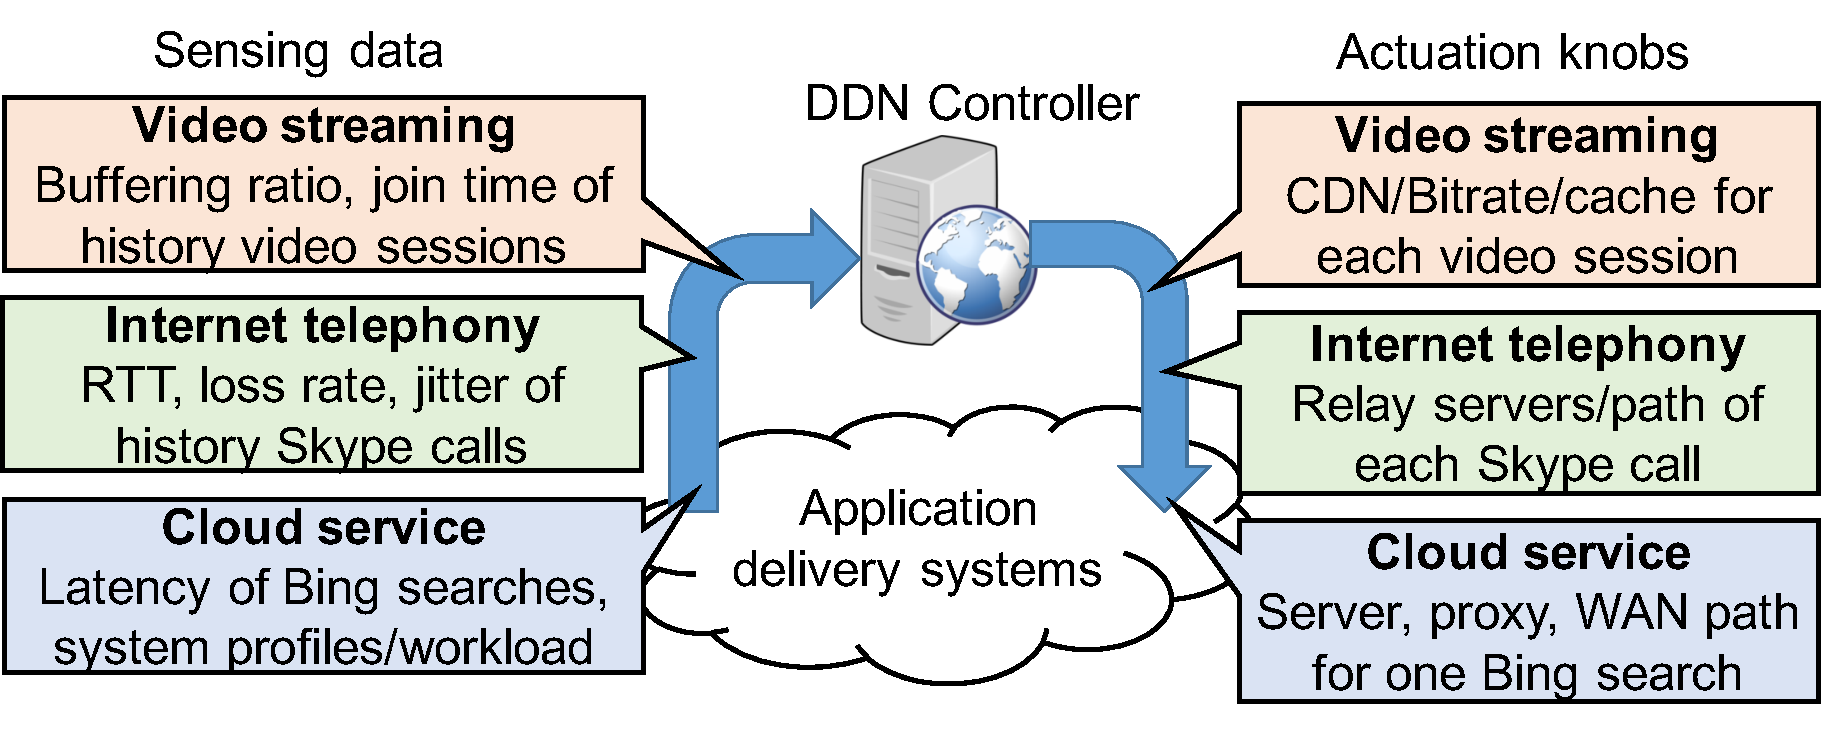
\includegraphics[width=0.8\textwidth]{figures/early-examples.pdf}
%%\vspace{-0.2cm}
%\caption{Examples of \ddn.}
%\label{fig:early-examples}
%\end{figure}



%\begin{figure}[t!]
%\centering
%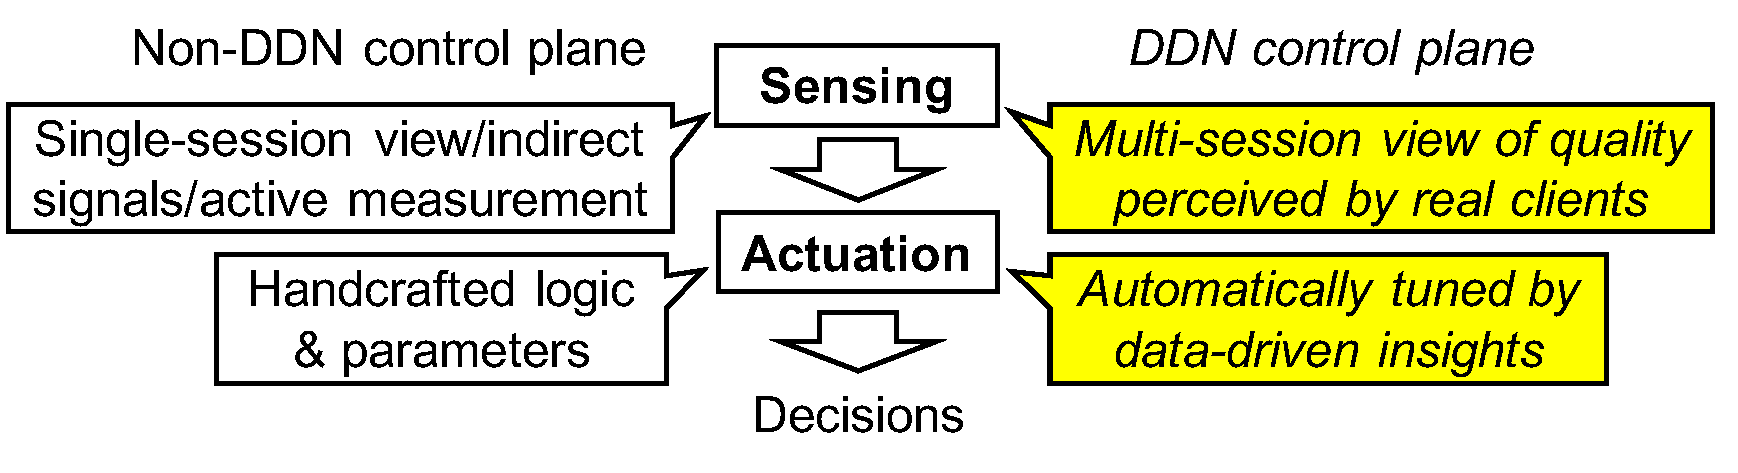
\includegraphics[width=0.8\textwidth]{figures/sensing-actuation.pdf}
%%\vspace{-0.7cm}
%\caption{\ddn control plane is fundamentally different to non-\ddn ones on both sensing and actuation.}
%\label{fig:sensing-actuation}
%\end{figure}


\section{Challenges}
\label{sec:overview:challenges}

While \ddn is promising,
it poses technical challenges on both 
algorithmic and architectural fronts, which have to be 
addressed before we can unleash its full potential.
%This section describes two fundamental challenges 
%of \ddn and how they manifest themselves in various
%applications.

\subsection{Need for Expressive Models}
\label{subsec:overview:challenge1}

Algorithmically, the objective of \ddn is to identify 
the best decision for each application sessions;
essentially, a mapping between the feature space
of application sessions and the decision space.
This is, however, by no means trivial even for 
standard machine learning techniques,
because the mapping is in a 
{\em high-dimensional} space.
Therefore, the key algorithmic challenge is 
how to build an expressive model to reduce
the dimensionality of both session-level 
feature space and decision space.
To make it more concrete, we discuss two
manifestations of the challenge of an expressive
model.

\begin{itemize}

\item {\em Complex QoE-determining factors:} 
The first example shows that the relation between
session-level features and video QoE is complex
both spatially and temporally.
Prior work has shown that there is a substantial room for 
improving video QoE by dynamically selecting the 
optimal CDN and bitrate based on a real-time global 
view of network conditions.
The key to realizing this promise is a prediction 
model that can accurately predict the quality of any 
video session based on QoE of similar sessions,
if it were to use any CDN and bitrate.
One challenge to practically build such prediction 
model is that video QoE has complex relationship to 
session-level features.
In particular, we observe a combinational effect
where QoE is affect by a specific combination 
of feature values, but does not appear to be 
correlated with any individual feature.
We also observe that QoE of different sessions 
may be affected with different feature combinations.
In addition to these spatial patterns, these 
QoE-determining factors, as well as QoE itself may
over time on timescales of several minutes.
Therefore a prediction model must be expressive
enough to capture all these spatial and temporal
complexities.

\item {\em Large decision spaces:}
The second example shows the problem of 
large decision spaces in Internet telephony.
Prior work has shown that there is much room 
for improving Skype quality by routing each 
call through the optimal relay clusters in 
the cloud.
%challenge
However, identifying a close-to-optimal relay 
in practice is very challenging, due to the sheer 
number of possible relay paths (in hundreds) and 
their dynamic performance (which could change 
on timescales of minutes). 
In addition, the number of calls different AS pairs
follows a highly skewed distribution, so that
in many AS pairs, the number of calls in each 
hour is even less than the number of possible 
relays.
Straightforward methods are not 
efficient to reduce the decision space.
For instance, focusing only on relays with 
the lowest geo-distance to end users
does not necessarily guarantee low latency, 
low packet loss rate which have been shown
to have weak, if any, correlation with the geo-distance.
Moreover, the best choice of relays depends 
on locations of both caller and callee.
All these evidences suggest a strong need
to reduce the size of the mapping between
the client space and the decision space in 
the context of today's VoIP architecture.

\end{itemize}



%\begin{itemize}
%\item From data to insights requires expressive models
%\item Example 1: predictive model
%\item Example 2: reducing decision space
%\end{itemize}

\subsection{Need for Scalable Platforms}
\label{subsec:overview:challenge2}

The system design of \ddn should meet the following requirements:
the \ddn controller has to make control decisions 
in near real time based on fresh data from many
other geo-distributed clients, and serve the decisions 
to clients within low response time.
The key architectural challenge, therefore,
is how to strike a balance between three seemingly
conflicting objectives: 
(1) {\em data freshness}, 
(2) {\em responsiveness to geo-distributed clients},
and (3) {\em global view}.
To make it more concrete, we again discuss two 
manifestations of the challenge of a scalable platform.

\begin{itemize}
\item {\em Geo-distributed analytics with global view:} 
The first example shows why it is challenging to 
make decision with a fresh, global view of QoE of 
many geo-distributed clients.
Although in theory, the \ddn controller can be 
integrated to the existing logically centralized control 
platforms deployed by many application providers,
there is a practical challenge: these control platforms 
are built up to serve two functions--
real-time per-session monitoring and 
offline analytics, neither of which requires a fresh 
and global data collected all clients, so it would be 
impractical to assume the decision-making algorithm 
can run in a cluster which has a fresh, global view 
of measurement data from all clients. 
Besides, it is costly to gather all data into one cluster,
because it requires to change the existing 
data gathering procedure and to significantly increase 
the communication overhead.
Therefore, one challenge is to 
perform geo-distributed analytics by striking a 
balance between global view and data freshness.

\item {\em Near real-time predictive analytics:}
Even if we can gather real-time data to the same data 
center, it is still very challenging to run real-time 
analytics to predict the optimal decision in near 
real time, e.g., on a timescale of tens of seconds.
As mentioned in 
Section~\ref{subsec:overview:challenge1},
to update quality prediction, we need a large amount 
of data to build a high-dimensional model between 
session-level feature space and QoE.
Our evaluation based on standard large-scale
analytics platforms has shown that it would take
tens of minutes, a magnitude longer than needed,
to update the model, given the sheer volume of
measurement data.

\end{itemize}

%\begin{itemize}
%\item From insights to real-time control requires scalable platform
%\item Example 1: Enabling complex real-time analytics
%\item Example 2: High responsiveness
%\end{itemize}


\section{Persistent Structures in QoE-Determining Factors}
\label{sec:overview:unifying}

%\jc{add a formal definition and illustrative figures of persistent structures}

Our solutions to address these challenges integrate 
standard ML algorithms and 
systems with a key domain specific insight that Internet
%Before we show how to address these challenges, 
%it would be helpful to  first understand the key domain-specific insight that
%inspires our solution.
%One unifying theme behind these seemingly 
%independent ideas is to integrate 
%standard machine learning algorithms and 
%systems with the domain-specific insight that Internet 
applications have {\em persistent structures
(e.g., performance bottlenecks) that help identify 
network sessions with 
similar QoE-determining factors, and that such 
structure tends to be persistent on timescales of 
at least tens of minutes}.
In Chapter~\ref{ch:measurement}, we will show evidence of these persistent
structures through an empirical structural analysis on  QoE
problems based on real datasets.
For now, we will give an overview of persistent structures 
and how intuitively they help address \ddn's challenges.

\mypara{Formal definition}
To formally describe the insight of persistent structures, 
let us formally describe \ddn as follows. In essence, \ddn is as 
a decision-making function
$F:2^\mathbb{S}\times2^\mathbb{D}\times\mathbb{S}\times\mathbb{R}
\mapsto\mathbb{D}$ which takes as input a set of historical 
sessions $S\in2^\mathbb{S}$ whose 
QoE is already measured, a set of available decisions 
$D\in2^\mathbb{D}$, a new session $s\in\mathbb{S}$, and $s$'s timestamp
$t\in\mathbb{R}$,
and outputs a decision $d\in\mathbb{D}$ for session $s$.
Then we formally define a {\em structure} as
a function 
$P:2^\mathbb{S}\times2^\mathbb{D}\times\mathbb{S}\times\mathbb{R}
\mapsto2^\mathbb{S}\times2^\mathbb{D}$,
which takes as input a pair of a set of historical 
sessions $S\in2^\mathbb{S}$ and a set of decisions $D\in2^\mathbb{D}$,
and a session $s\in\mathbb{S}$, and the timestamp
$t\in\mathbb{R}$, and outputs a pair of  subset of history sessions
$S'\subset{S}$ and a  subset of available decisions $D'\subset{D}$.



\mypara{Key properties}
Persistent structures have two key properties:

\begin{itemize}

\item {\em Criticality:} Spatially, these structures identify (often small) 
subsets of history
sessions and decisions which are more critical than others history sessions 
or decisions in determining QoE; i.e.,
$F(S,D,s,t)=F(S',D',s,t)$, where $(S',D')=P(S,D,s,t)$. This essentially
means the \ddn control logic can make almost the same decisions by
focusing on a subspace of relevant history sessions and decisions.

\item {\em Persistence:} Temporally, these structures tend to persist
on timescales of tens of minutes. This means in a time window $\Delta$ 
of  tens of minutes, the function $P$ is likely 
to find the same relevant history sessions and decisions,
i.e., $P(S,D,s,t)=P(S,D,s,t+\Delta)$.

\end{itemize}


\mypara{An example}
These persistent structures of QoE-determining factors can 
manifest themselves in many forms.
For instance, if the QoE of a video session depends on
the server load (i.e., some decision-specific properties)
and client-side ASN (i.e., some session-level features), and such
dependency lasts for tens of minutes,
then it would be possible to identify the best decision for
the session by looking
at history sessions having in the same AS 
(instead of all history sessions), and only consider server with 
low load (instead of all possible decisions).

\mypara{Intuition behind persistent structures}
The intuitive explanation of these persistent structures 
is that in networked systems and application delivery  systems, performance
bottlenecks are often persistent, and the persistent structures
can be viewed as ``manifestations'' of these bottlenecks in the space of 
session-level features and decision-specific properties--a session's QoE
only depend on history sessions and decisions 
experiencing the same bottleneck.
Such persistent bottlenecks can be found in many prior studies in the context
video streaming~\cite{cfa}, 
web service~\cite{footprint}, end-to-end
network performance~\cite{zhang2001constancy}.
They can also be viewed as a generalization of the persistent 
network congestions, which can be mathematically explained based on queueing theory
(Chapter 6 of \cite{keshav2012mathematical}).

% For instance, video
%sessions with similar QoE from the same CDN/server tend to match on 
%client IP prefix~\cite{cfa,cs2p}. 
%Similarly, VoIP calls between the same ASes are likely to share the best
%relays~\cite{via},  and clients from  same /24 IP prefix will have
%similar web load time from the same edge proxy~\cite{footprint}.

%which takes as input a given set of historical 
%sessions $S\in2^\mathbb{S}$ and a new session $s\in\mathbb{S}$,
%and outputs a subset of history sessions $S'\subset{S}$; 
%and $L:2^\mathbb{D}\times\mathbb{S}\mapsto2^\mathbb{D}$, 
%which takes as input a given set of available decisions
%$D\in2^\mathbb{D}$ and a new session $s\in\mathbb{S}$,
%and outputs a subset of these decisions $D'\subset{D}$.


%For instance, the persistent critical features 
%(Section~\ref{subsec:overview:cfa}) can be
%viewed a kind of persistent structure which
%groups video sessions that match values on
%their critical features.
%The fact that there is a stable subset of 
%promising relay choices for each AS pair 
%(Section~\ref{subsec:overview:guided}) 
%can be viewed as another example of 
%persistent structure, where the structure
%is the subspace of the large decision space.

\mypara{Why they are helpful}
Persistent structures are the key
enabler for our design of expressive models and scalable
systems for \ddn.
\begin{itemize}

\item First, the locality property of these domain-specific structures 
means they are in relatively low dimensional space.
%(e.g., in Section~\ref{subsec:overview:cfa}, 
%critical features are a small subset of all
%session-level features). 
Therefore, we can build models that focus on these 
domain-specific structures, so that 
they are expressive enough to capture the complex relations 
between session-level features
and decisions with limited available data, 
while avoiding using unnecessarily high-dimensional models.
This idea in spirit is similar how ``locality''
is used in many machine learning techniques 
to tackle curse of dimensionality~\cite{ml101}.

\item Second, in the context network applications,
these structures often correlate with network locality (e.g., clients 
in the same IP prefix). Therefore, they enable an effective spatial 
decomposition of the global 
data-driven process into smaller-scale 
subprocesses, each controlling a subset of 
sessions who share network locality.
% (i.e., can be mapped
%to the same subspace of relevant history sessions and decisions.
%(as in group-based exploration-exploitation of 
%Section~\ref{subsec:overview:group})
%or a subset of decisions (as in guided 
%exploration of 
%Section~\ref{subsec:overview:guided}).

\item Third, since these structures tend to
persist on longer timescales than QoE itself 
does, we can learn these structures from
more history data 
%(as in critical feature analysis of
%Section~\ref{subsec:overview:cfa} 
%and guided exploration of 
%Section~\ref{subsec:overview:guided}) 
with an
offline process separate from real-time 
decision making.
%(as in group-based 
%exploration-exploitation of
%Section~\ref{subsec:overview:group}).

\end{itemize}


\section{Key Ideas}
\label{sec:overview:solutions}

This section briefly describes three key ideas inspired by 
persistent structures
to address the aforementioned challenges. 
Figure~\ref{fig:overview-roadmap} summarizes the 
the mapping between the challenges and the ideas.
%We conclude the section by discussing a unifying
%insight underlying these solutions.

%of 
%{\em persistent structures--there exist some structure
%(e.g., performance bottlenecks) that identifies 
%network sessions with 
%similar QoE-determining factors, and that such 
%structure tends to be persistent on timescales of 
%tens of minutes}.
%The term ``structure'' is broadly defined, and will 
%have specific meanings when we discuss it in 
%context.
%Next, we will briefly describe how the persistent
%structures 

\begin{figure}[t!]
\centering
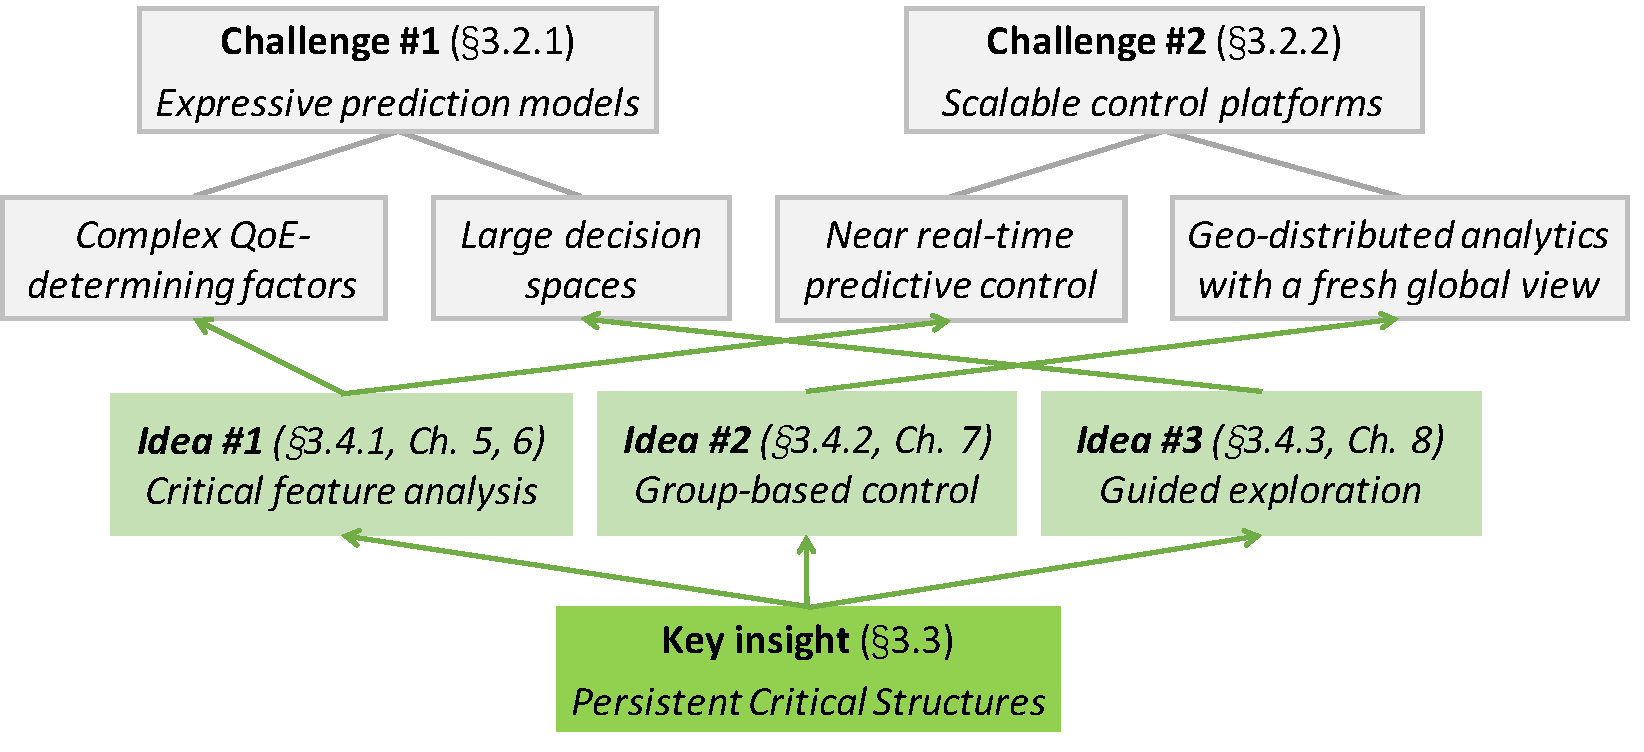
\includegraphics[width=0.95\textwidth]{figures/overview-roadmap.pdf}
%\vspace{-0.3cm}
\caption{Roadmap of the dissertation.
The figure shows that the unifying insight inspires 
our three key ideas to address four manifestations of
\ddn's key algorithmic and architectural challenge.}
\label{fig:overview-roadmap}
\end{figure}

\subsection{Critical Features Analysis}
\label{subsec:overview:cfa}

As we have seen, video QoE can be improved by
a prediction system that accurately predicts the QoE 
of a video session if it uses a certain CDN and bitrate.
The challenge is that this prediction system must be 
(a) expressive enough to capture complex relations 
between video quality and observed session features, 
and (b) capable of updating quality predictions in near 
real time.
We used several off-the-shelf machine learning 
techniques, such as random forests and SVM, but 
found they did not produce expected QoE improvements, 
because the long-term historical data is too coarse grained 
for these algorithms to capture the dynamics of video 
quality, while the short-term historical data is not sufficient 
for the algorithms to learn complex relations between 
video quality and observed session features.

Our solution leverages an instantiation of persistent structures
in video streaming, called 
{\em persistent critical features: each video session has 
a small set of critical features that ultimately determines 
its video quality, and these critical features change much 
more slowly than video quality}. 
Let us consider a concrete example of such persistent 
critical features from~\cite{cfa}.
In a real-world incident, video sessions of Comcast
users in Baltimore who watched videos from Level3
CDN experienced high failure rate (VSF) for several
hours. The reason turned out
to be the overloaded local cluster serving Comcast
users in that area,
which can be characterized by three critical features: 
CDN (``Level3''), ASN (``Comcast'') and City (``Baltimore''),
and the correlation between the combination of these
feature values and high VSF persist for the whole
duration of this incident, even though the QoE
has fluctuated a lot during this period.

The insight of persistent critical features has inspired
a prediction model that captures complex QoE-determining 
factors and is amenable to scalable implementation.
Given a video session under prediction, the model 
identifies many similar sessions from a short-term 
history by matching only on its critical features,
thus capturing complex QoE determining factors
while avoiding curse of dimensionality.
The persistence of these critical features also naturally
enables decoupled implementation: 
we can learn these critical features from long-term historical 
data and update the models by short-term historical data 
in near real time to capturing quality fluctuation.


%%\paragraph{CFA: Improving QoE via Expressive Prediction Models.}
%%problem
%Delivering high QoE is crucial to the success of today's subscription-/ad-based business models for Internet video.
%There is substantial room for improving video QoE by dynamically selecting the optimal CDN (Content Delivery Network) and bitrate based on a real-time global view of network conditions~\cite{sigcomm-case,conext-shedding}.
%The key to realizing this promise is a {\em prediction oracle} that can accurately predict the quality of a video client if it uses a certain CDN and bitrate.
%%challenge
%The challenge is that this prediction system must be (a) expressive enough to capture complex relations between video quality and observed session features, and (b) capable of updating quality predictions in near real time.
%We used several off-the-shelf machine learning techniques, such as random forests and SVM, but found they did not produce expected QoE improvements, because the long-term historical data is too coarse grained for these algorithms to capture the dynamics of video quality, while the short-term historical data is not sufficient for the algorithms to learn complex relations between video quality and observed session features.
%%these algorithms fail to capture the quality variability when trained with long-term history data, and they fail to identify the complex prediction models when trained with short-term history data.
%%Unfortunately, several seemingly natural solutions (e.g., simple machine learning approaches and network models) fail on one or both fronts.
%%insight
%My solution, CFA~\cite{cfa}, leverages the domain-specific insight of {\em persistent critical features}; each video session has a small set of critical features that ultimately determines its video quality, and these critical features change much more slowly than video quality~\cite{conext-shedding}. 
%%I present the design and implementation of CFA~\cite{cfa} to address these challenges. 
%%CFA is driven by the domain-specific insight of {\em persistent critical features}, that each video session has a subset of critical features that ultimately determines its video quality, and these critical features tend to be persistent on timescales of tens of minutes~\cite{conext-shedding}. 
%%solution
%This insight enables us to learn complex prediction models from long-term historical data (thus expressing complex relations between video quality and session features), and update the models by short-term historical data in near real time (thus capturing quality fluctuation as well).
%%Therefore, CFA can predict video quality more accurately than many machine learning algorithms, though CFA may not be as good in other prediction tasks.
%%result
%A real-world pilot deployment shows that CFA leads to non-trivial improvements in video quality, e.g., 32\% less buffering time than industry-standard algorithms.
%Our conversation with domain experts confirmed that these improvements are significant for content providers and can potentially translate into substantial benefits in revenues.
%An end-to-end implementation of CFA has been deployed and used by Conviva, a company that offers video quality optimization services to many premium content providers. 
%
%The insight of persistent critical features turns out to be more general; e.g., I have also applied the same insight to accurate prediction of TCP throughput~\cite{cs2p}, which leads to 11\% higher video bitrate than state-of-the-art adaptive bitrate players (e.g., Netflix players) with no extra buffering.


\subsection{Group-Based Control}
\label{subsec:overview:group}

While the predictive decision-making algorithm 
described above shows promising QoE improvement, 
it faces has two fundamental limitations.
(a) Casting the data-driven QoE optimization as a
prediction problem suffers from the many known 
biases such as incomplete visibility.
%A natural solution is to re-cast the problem
%as a real-time exploration and exploitation process,
%which however, is not trivial due to the fact that 
%measurement data of one client is useful only
%to the clients sharing the same QoE-determining
%factors.
(b) The prediction algorithm is not a geo-distributed one, 
so it requires a fresh and global view be maintained in
one cluster. Having a fresh and global view 
physically in the same cluster is, however, impractical 
because in many control platforms, measurement 
data are first collected in several geo-distributed frontend 
clusters each having a partial view of nearby clients,
and then periodically archived in a backend cluster
to form a global though slightly staled view.
A baseline approach is to run control logic in a 
single backend cluster with global data from frontend 
clusters, but this approach leads to non-trivial 
staleness of the global data and suboptimal decisions.


To overcome these limitations, we re-cast the 
data-driven QoE  optimization as a real-time 
exploration and exploitation process, and build 
a practical system to run it among all clients at 
scale. 
Our key insight is inspired by the criticality of persistent
structures -- {\em the clients that exhibit similar 
QoE behavior will have similar network-level 
features (e.g., same IP prefix), and thus their 
fresh data will likely be collected by the same 
frontend cluster.}
We see manifestations of this insight in many 
settings.
% When clients share certain location or IP prefix-related
%features, they are more likely to have the similar video QoE~\cite{cfa} and
%similar TCP throughput~\cite{cs2p,spand} at the same point of time. 
For instance, video sessions with similar QoE 
from the same CDN/server tend to match on 
client IP prefix~\cite{cfa,cs2p}. 
Similarly, VoIP calls between the same ASes 
are likely to share the best
relays~\cite{via},  and clients from  same /24 
IP prefix will have
similar web load time from the same edge 
proxy~\cite{footprint}.

This insight inspires the notion of {\em group-based 
control}, which enables the real-time global 
exploration-exploitation process by decomposing 
the process into subprocesses, each controlling 
a group of clients with similar context by
network locality and other key session-level features 
and running in the frontend cluster that has these 
clients' fresh data.
Since sessions within a group share network locality (e.g., 
in the same locations and IP prefixes), 
they are likely to be mapped to the same frontend cluster.
By running the per-group exploration-exploitation 
logic in this frontend cluster, we can update
decisions with fresh data from other sessions i
n the group received by this frontend cluster.


%%\mypara{\underline{\smash{Real-Time Exploration and Exploitation At Scale.}}}
%%\paragraph{Pytheas: Improving QoE via Exploration and Exploitation at Scale.}
%%\mypara{Real-Time Exploration and Exploitation at Scale:}
%%problem
%While formulating data-driven QoE optimization as a prediction 
%problem has shown promising QoE improvement (e.g., CFA), 
%it is necessarily incomplete, as 
%it suffers from many known biases such as incomplete visibility, 
%and cannot respond to sudden changes such as flash crowds.
%Drawing a parallel from machine learning (e.g., ad recommendation), I argued that data-driven QoE optimization should instead be cast as a {\em real-time exploration and exploitation} process. % rather than as a prediction problem. 
%Measurement collection (exploration) could be informed by decision making (exploitation) to explore the decisions with less data, thus addressing the shortcomings of the prediction-based formulation.
%This new formulation is complementary to CFA, since CFA's prediction model can be reused to capture similarities among clients.
%%challenge
%While many exploration-and-exploitation algorithms are available, enabling these algorithms in networking introduces an architectural challenge: we need a {\em scalable control platform} to update decisions with fresh global data from clients, despite data coming from a variety of geo-distributed front-end clusters, each with only a partial view of the clients.
%%The key challenge of real-time exploration and exploitation in networking is how to update decisions in real-time for millions of geo-distributed clients using their fresh measurement data.
%%insight
%A baseline approach is to run control logic in a single back-end cluster with global data from front-end clusters, but this approach leads to non-trivial staleness of the global data and suboptimal decisions.
%I take an alternative approach; the control logic is run by geo-distributed front-end clusters which have fresh data, rather than the back-end cluster.
%The intuition is that the clients that exhibit similar QoE behavior will have similar network-level features (e.g., same IP prefix), and thus their fresh data will likely be collected by the same front-end cluster.
%%While the challenge might be intractable in a general setting, it
%%I address the challenge by the insight that network application sessions sharing the same {\em network- and application-level features} intuitively exhibit similar QoE behavior across different possible decisions.
%%solution
%Inspired by this insight, {Pytheas}~\cite{pytheas} uses the concept of {\em group-based exploration and exploitation}, which 
%%The key idea is to decompose the global exploration and exploitation process of all clients into processes within groups of similar clients and run these per-group processes in geo-distributed front-end clusters which are close to clients and have their fresh data.
%%The key idea is to decompose the global exploration and exploitation process into subprocesses of similar clients, and run each subprocess by the front-end cluster that is close to its clients and has their fresh data.
%decomposes the global exploration and exploitation process into subprocesses, each controlling a group of similar clients and running in the front-end cluster that has these clients' fresh data.
%%with both client-closeness and data-freshness.
%%result
%Using an end-to-end implementation in CloudLab, I show that compared to a state-of-the-art prediction-based system, Pytheas improves the average video QoE by up to 31\% and the 90th percentile QoE by 78\%.
%Pytheas is an open source project that enables application providers to deploy the proposed architecture at scale within their existing infrastructure. 


\subsection{Guided Exploration}
\label{subsec:overview:guided}

To make data-driven QoE optimization practical in Internet telephony,
we have to address an additional challenge that it has a 
large decision space of relay choices, so there 
are usually not enough VoIP calls to reliably estimate 
the dynamic network performance between each 
AS pair.

The key insight to address this challenge is  another
illustration of persistent structure --
{\em the stability of promising relay choices: for each pair of 
caller AS and callee AS, there is a small and 
stable subset of relays that almost always 
contains the best relay}. 
This insight has two implications: 
(1) because this subset of relays is stable, 
it can be learned from history; and 
(2) because this subset has only a few relays 
(less than five), it can be explored efficiently 
even with limited data.
Inspired by this insight, we develop a relay selection 
system that achieved close-to-optimal quality 
using the concept of {\em guided exploration}. 
The idea is to learn a small set of promising relays 
for each AS pair based on long-term (e.g., daily) 
historical data, and explore these relays using most
calls in real time.

%%\mypara{\underline{\smash{Reducing Large Decision Space.}}} 
%%\paragraph{VIA: Improving QoE in the Face of Large Decision Spaces.} 
%%\mypara{Reducing Large Decision Space:}
%%problem
%In the first large-scale study on Internet telephony quality, I found that a substantial fraction of Skype calls suffer from poor network performance, and that there is much room for improving Skype quality by routing each call through the optimal relay clusters in Microsoft's cloud.
%%challenge
%However, identifying a close-to-optimal relay in practice is very challenging, due to the sheer number of possible relay paths (in hundreds) and their dynamic performance (which could change on timescales of minutes). 
%Neither prediction-based methods (e.g., CFA) nor those based on exploration and exploitation (e.g., Pytheas) suffice to handle such a large decision space.
%%insight
%The key insight to address this challenge is that, for each pair of caller ISP and callee ISP, there is a {\em small and stable subset} of relays that almost always contains the best relay. 
%This insight has two implications: (1) because this subset of relays is stable, it can be learned from history; and (2) because this subset has only a few relays (less than five), it can be explored efficiently even with limited data.
%%the large decision space can be narrowed down to a {\em small subset} of relays that almost always contains the best relay, and such pruning can be learned from the historical data, because this set of most promising relays tends to be {\em persistent}.
%%solution
%Inspired by these intuitions, I developed {VIA}~\cite{via}, a relay selection system that achieved close-to-optimal quality using the concept of {\em guided exploration}. The idea is to learn a small set of promising relays for each ISP pair based on long-term (e.g., daily) historical data, and explore these relays using most calls in real time.
%%result
%Trace-driven analysis and a small-scale deployment shows that VIA cuts the incidence of poor network conditions for calls by 45\% (and for some countries and ISPs by over 80\%) compared to today's Skype quality.
%VIA has been used in Microsoft internal deployment with real Skype users, and is in the process of being fully deployed. 
%VIA was also used by Microsoft to identify the countries and ISPs where Skype quality can benefit the most if relaying services are deployed.
%%VIA is also used to identify the countries and ISPs where Skype quality can benefit the most from Microsoft relaying services.


%\subsection{How Persistent Structures Are Used}
 


\section{Summary}

In this section, we have discussed the advantages
of \ddn over prior approaches. 
In particular, as an application-level endpoint 
approach, \ddn enjoys the advantage of direct 
access to user-perceived QoE, and at the same
time, compensates the limited insight to network 
conditions by consolidating real-time measurement
from many endpoints, thus achieving the best world
of both endpoint solutions and in-network solutions.

We have also presented an overview of our solutions
to address \ddn's technical challenges--the need for 
expressive models and scalable systems. 
In particular, there are the three key ideas underlying 
our solutions: 
(1) critical feature analysis to enable an expressive 
QoE prediction model, 
(2) group-based control to enable real-time 
exploration-exploitation process at scale, and
(3) guided exploration to handle the large 
decision spaces in Internet telephony.
Finally, we summarize the section by distilling 
a unifying insight from these 
ideas--\ddn can be made practical by integrating
machine learning with the insight that there are 
persistent domain-specific structures.









\chapter{Structural Analysis of QoE Problems}
\label{ch:measurement}

%We have seen that the limitations of prior approach have caused 
%pervasive QoE problems in the wild (Chapter~\ref{ch:related}),
%and this dissertation seeks to improve QoE by exploring a 
%new data-driven approach which leverages the QoE information 
%observed by millions of sessions in real time (Chapter~\ref{ch:overview}).
%The key insight to make such data-driven QoE optimization practical
%is the observation that there are {\em persistent structures in the 
%QoE-determining factors} (Section~\ref{sec:overview:unifying}).

We have seen that \ddn is a promising alternative to overcoming the fundamental 
limitations in prior work of QoE optimization, and the key insight to make \ddn practical
is the {\em persistent critical structures in the QoE-determining factors}.
In this chapter, we present empirical evidence of these persistent critical structures by 
using a large-scale structural analysis on the video and VoIP QoE.
In particular, we shed light on the {\em temporal persistence} and {\em spatial criticality}
of these structures of QoE-determining factors in the wild.
%To this end, our analysis focuses on the spatial and temporal patterns
%of QoE problems.
\begin{itemize}


\item {Spatial patterns:} 
Are the QoE problems uniformly spread through the 
space of feature combinations or are there specific 
combinations that have a higher concentration?

\item {Temporal patterns:} 
Is each QoE problem a transient for 
a specific ISP, CDN, or provider (or combination of these) or are 
these problems persistent over long periods?


\end{itemize}
We also show that there are substantial correlations
among the QoE problems of different metrics, suggesting that
it is possible to improve multiple QoE metrics simultaneously.

This chapter is organized as follows. 
Section~\ref{sec:measurement:video} presents the structural analysis
on video QoE,
Section~\ref{sec:measurement:voip} presents a similar analysis on 
VoIP QoE, and Section~\ref{sec:measurement:summary} summarizes
the chapter with key observations.


%The key role that QoE plays in impacting user engagement,
%and consequently providers' revenues, has motivated recent
%efforts, including this dissertation, in improving the QoE of 
%Internet applications like
%Internet video and Internet telephony.
%Before we embark on designing and deploying new 
%schemes to improve QoE, we need to first understand 
%the nature of QoE problems.
%To this end, this section uses large-scale datasets collected
%from real users to shed light on the structure of today's 
%QoE problems  in the wild.
%In particular, we observe that 
%(1) a substantial fraction of video and VoIP 
%sessions suffer from QoE problems; and
%(2) QoE problems exhibit patterns both 
%spatially (e.g., correlation to
%certain client-side features) and temporally
%(e.g., prevalent/persistent quality issues).
%
%This chapter is organized as follows.
%Section~\ref{sec:measurement:video} presents a 
%measurement study on video QoE.
%Using 300 million video sessions collected over a 
%two-week period, we show how severe today's
%QoE problems are, and  analyze the spatial
%and temporal properties of these QoE problems.
%Section~\ref{sec:measurement:voip} presents
%a similar measurement study on Internet telephony 
%QoE based on a dataset from one of the most 
%popular VoIP  service providers.
%Finally, Section~\ref{sec:measurement:summary} 
%summarizes the chapter with key findings 
%which motivate the ideas proposed in later 
%chapters.


\section{Internet Video}
\label{sec:measurement:video} 

\newcommand{\numsessions}{numsessions\xspace}
\newcommand{\problemsession}{problem session\xspace}
\newcommand{\problemsessions}{problem sessions\xspace}
\newcommand{\cluster}{cluster\xspace}
\newcommand{\clusters}{clusters\xspace}
\newcommand{\problemcluster}{problem cluster\xspace}
\newcommand{\problemclusters}{problem clusters\xspace}
\newcommand{\problemratio}{problem ratio\xspace}

\newcommand{\criticalcluster}{critical cluster\xspace}
\newcommand{\criticalclusters}{critical clusters\xspace}

%In this section, we begin by describing our dataset and
%metrics under consideration.
%Then we present preliminary statistics on today's 
%video QoE to motivate 
%the types of structural insights we would
%like to obtain regarding the nature of video 
%quality problems. 
In this section, we begin by describing our dataset and
the methodology of analyzing spatial and temporal patterns
of video QoE problems 
(Section~\ref{subsec:measurement:video:method}),
then present our results in 
Section~\ref{subsec:measurement:video:spatial},
~\ref{subsec:measurement:video:temporal}, and
~\ref{subsec:measurement:video:correlation},
and finally summarizes the observations in 
Section~\ref{subsec:measurement:video:discuss}.

\subsection{Methodology}
\label{subsec:measurement:video:method}

\mypara{Dataset}
We use the same dataset as described in 
Section~\ref{subsec:related:video-qoe}. 
The dataset consists of client-side measurements of
video  quality from over 300 million sessions of 
379 distinct content providers spanning diverse
genres, both live and video-on-demand content, different
content delivery platforms, different types of  bitrate adaptation
algorithms, and device/browser platforms.

\mypara{Session-level features}
The basic unit in our dataset is a video session. 
A session represents a user viewing a video on one of 
our affiliates' sites for some duration of time.
Each session is associated with a set of \emph{seven 
features}: 
\begin{packedenumerate}
\item \emph{ASN:} The Autonomous System Number 
(ASN) that the client IP belongs  to. 
Note that a single ISP (e.g., Comcast) may own 
different ASNs both  for management and business reasons. 
We focus on the ASN as it is more fine-grained
than the ISP granularity.  We observe in aggregate 
15K unique ASNs spanning multiple countries. 

\item \emph{CDN:}   In total, we observe 19 unique CDNs 
spanning popular CDN providers as well as several in-house 
and ISP-run CDNs. (Some providers use proprietary 
CDN switching logic; in this case we pick the segment of 
the session with the CDN used for the longest
duration.)


\item \emph{Content provider (Site):} This is the specific 
provider from which the client requested some content. 
We have  379 content providers that span different 
genres of content.  We use the terms site and
content provide interchangeably.

\item \emph{VoD or Live:} Video  content  falls in one 
 of two categories: video-on-demand (VoD) or Live.  
 We use a binary indicator to see if the particular
  content was a Live event or a 
 VoD video. 


\item \emph{Player type:} We see diverse  players 
such as  Flash, Silverlight, and HTML5.

\item \emph{Browser:} We see diverse client browsers 
including Chrome, Firefox, MSIE, and Safari. 

\item \emph{Connection type:} Finally, we  have the 
type of access network connection such  as
 mobile/fixed wireless, DSL, fiber-to-home. 
These annotations come from third party services~\cite{quova}.
 
\end{packedenumerate}

%Now that we see that many video sessions suffer from bad QoE, 
%we would like to know whether there is any patterns of these 
%video quality problems.
%In particular, we are interested in the temporal and spatial patterns 
%of QoE problems:
%\begin{itemize}
%\item Temporally, is each problem a transient or one-off event for 
%a specific ISP, CDN, or provider (or combination of these) or are 
%these problems persistent over long periods?
%\item , are the problems uniformly spread through the 
%space of feature combinations or are there specific 
%combinations that have a higher concentration?
%\end{itemize}

\mypara{Identifying problem sessions} 
Our focus  is on understanding quality problems as they appear 
in the wild. 
To this end, we identify \problemsessions w.r.t. each of the 
quality metrics. Note that a given session may appear as a 
\problemsession on a subset of  metrics; i.e., it might have a low
join time but may have a high buffering ratio or vice versa. 
We consider the  metrics separately to avoid implicitly 
assuming that the metrics or failures are correlated.

\begin{packeditemize}
\item For join failures, we use a binary indicator if the 
session failed or not.  
For the remaining metrics, we choose specific 
thresholds based on domain-specific
knowledge and observations in prior work\footnote{
We do acknowledge that there is no ideal choice of 
threshold and it is likely that these thresholds will evolve 
as user expectations and network conditions improve. 
As such, the choice of thresholds is illustrative of the 
structure of video quality problems that occur today. 
The methodology and qualitative observations we 
present are not  tied to the  specific  thresholds.
We have confirmed that the results are qualitatively 
similar for other choices  of these thresholds as well. }.  
Our specific thresholds and rationale are follows.
\item For buffering ratio, we identify a \problemsession 
if the value is greater than 5\%; this is based on the 
observation that beyond this value there is a sharp 
decrease in amount of video viewed~\cite{sigcomm11}.  
\item For bitrate, we mark a \problemsession if the average
bitrate is less than 700kbps; this value roughly
 corresponds to the recommended ``360p'' setting on 
 video providers. 
We use a fixed threshold of bitrate in this work for 
simplicity, but we do acknowledge that bitrate settings 
are content-dependent (e.g., some contents do not provide 
high resolution streams).
\item Third,  we mark all sessions with a join
time greater than 10 seconds; this represents a 
conservative upper bound on the
tolerance of users~\cite{webhci1,akamai-imc12}.  
\end{packeditemize}

\mypara{Identifying problem clusters}
 We begin by dividing our dataset into discrete one 
 hour epochs.\footnote{One hour is the finest 
 granularity of the dataset and thus we cannot 
 analyze effects at smaller timescales.} As a
first step to analyze the structure, we 
\emph{cluster}\footnote{The term ``cluster'' represents a 
group of sessions that share common features, and it is 
indeed  different from traditional   clustering algorithms 
where a cluster can be a group of any data points.} 
together sessions that share one or more client/session 
features within the same epoch.   
For instance, the \cluster ``ASN=$\mathit{ASN1}$'' describes 
all sessions where the user belongs
to $\mathit{ASN1}$ and the cluster 
``ASN=$\mathit{ASN1}$, CDN=$\mathit{CDN1}$'', 
describes all sessions where the
user belongs to $\mathit{ASN1}$ and the session was 
assigned to a server from $\mathit{CDN1}$.
In order for our observations to be reliable, 
we want to focus on  clusters that are deemed to be 
statistically significant sources of problem sessions. 
To this end, we define the \problemratio of a
cluster as the ratio 
$\frac{\textrm{\# of \problemsessions}}{\textrm{\# of
sessions}}$. Then, we cull out the \clusters whose 
\problemratio is
significantly higher than the global average \problemratio.  
We also remove all \clusters that have a small number 
of sessions in aggregate; i.e., problems observed within a 
small cluster may not be statistically significant.
Combining these two steps, we define a \problemcluster 
as a \cluster that has a \problemratio $\geq 1.5 \times$ the
global \problemratio,\footnote{This value roughly represents 
two standard deviations away  from the mean of the
per-cluster \problemratio distribution.}  and the number of 
sessions in this cluster is $\geq1000$.  
In the rest of this paper, we start from the \problemclusters 
as our basis and subsequently refine the analysis.

 
\begin{figure}[t!]
\centering
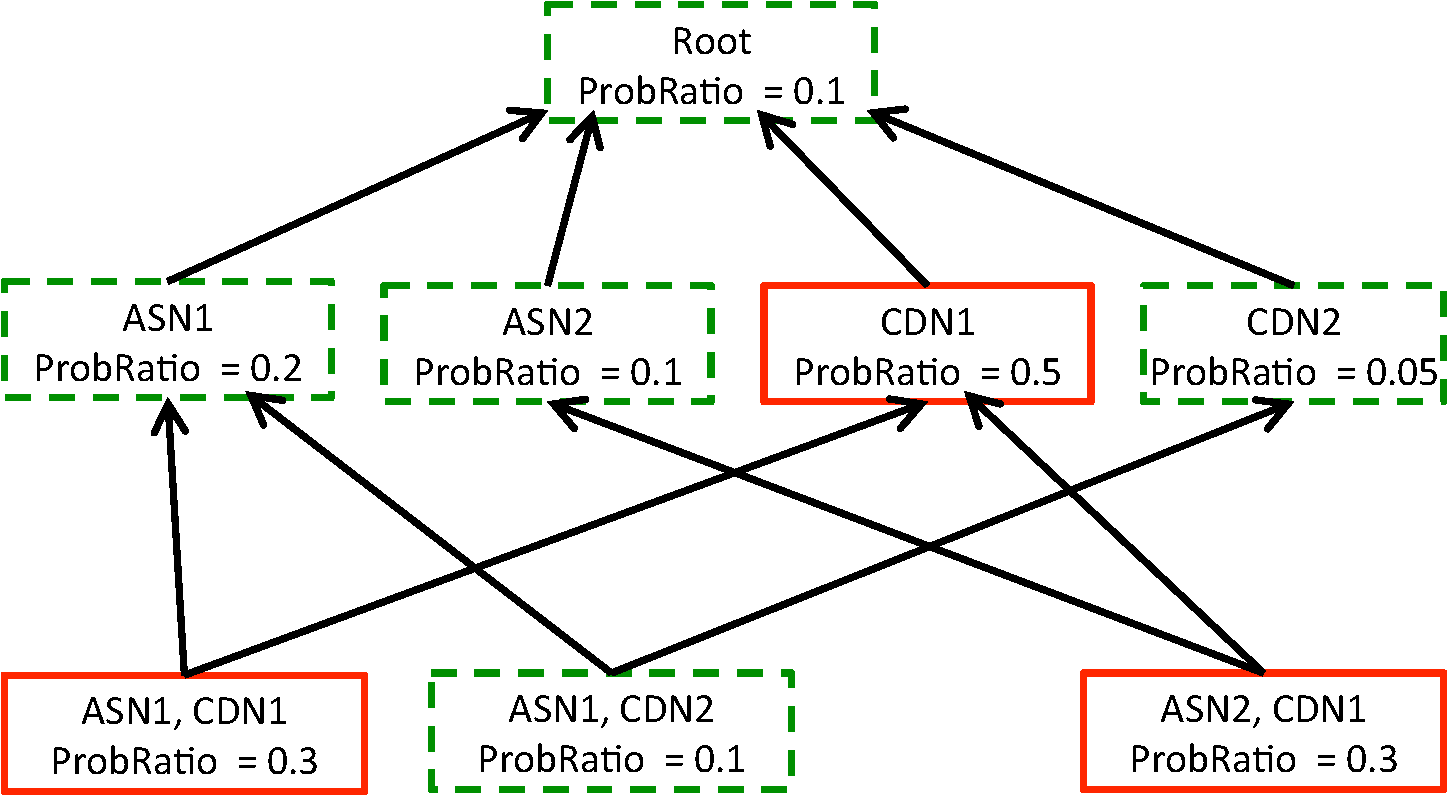
\includegraphics[width=0.7\textwidth]{figures/conext13-criticalcluster.pdf}
%\vspace{-0.3cm}
\caption{Representing the relationship between clusters using a DAG.  
Red boxes represent the \problemclusters.
%The dashed-green boxes show clusters without a high \problemratio and the solid-red boxes identify the \problemclusters.
}
\label{fig:method:critcluster}
\end{figure} 

%\begin{figure*}[t]
%\centering
%\captionsetup[subfigure]{justification=centering,farskip=-1pt,captionskip=5pt}
%\subfloat[Representing the relationship between clusters using a DAG.  
%Red boxes represent the \problemclusters.
%%The dashed-green boxes show clusters without a high \problemratio and the solid-red boxes identify the \problemclusters.
%]{
%   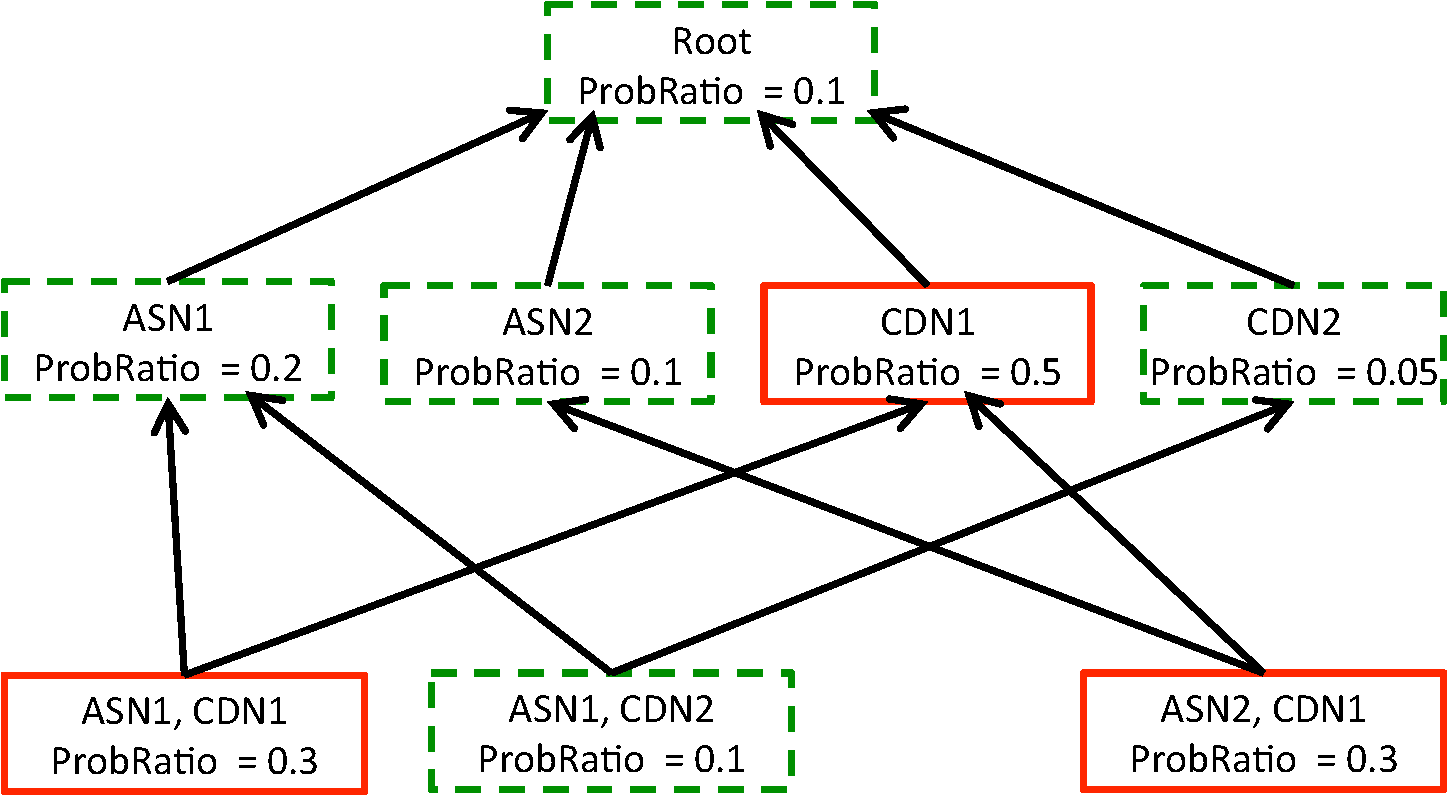
\includegraphics[width=0.6\textwidth] {figures/conext13-criticalcluster.pdf}
%   \label{fig:method:critcluster}
% }
%% \hspace{0.4cm}
%\\
%\subfloat[An illustration of the phase transition idea for  identifying a \criticalcluster. 
%%Intuitively,  removing any one feature from this \criticalcluster will cease to 
%%be a \problemcluster and adding any feature  to it will continue to be a \problemcluster.
%]{
%   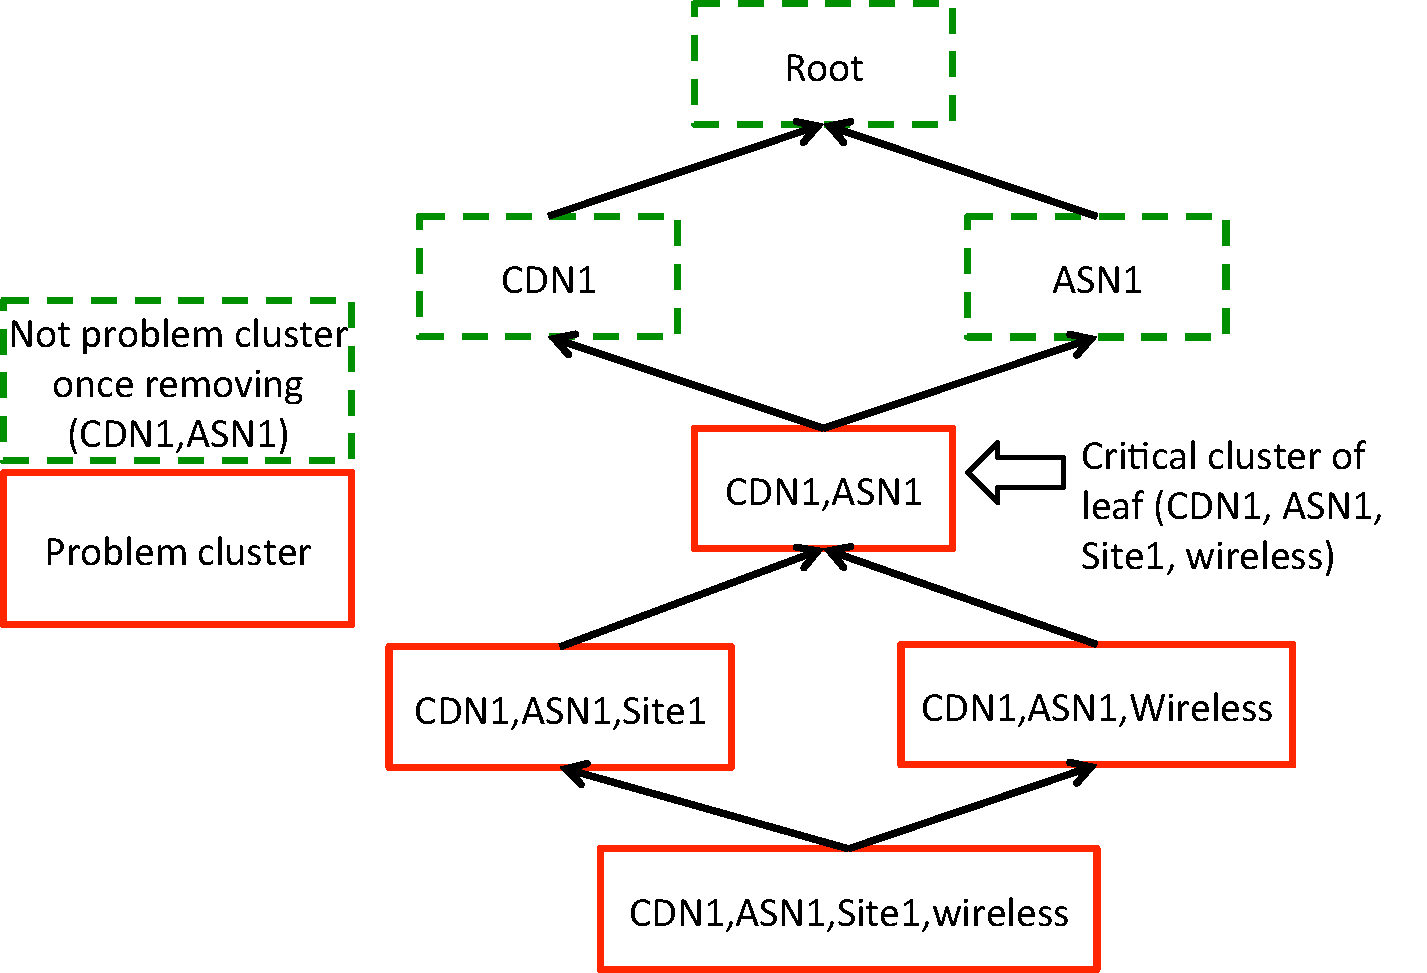
\includegraphics[width=0.6\textwidth] {figures/conext13-criticalcluster_example.pdf}
%   \label{fig:method:critclustr2}
% }
%\caption{Illustrative examples of how to identify \criticalclusters from \problemclusters.}
%\label{fig:pattern:method}
%\end{figure*}

While the grouping of problem sessions into \problemclusters  
provides some insights into the structure of problems, 
there is still one key missing aspect. 
Specifically, we may have different granularities of \problemclusters
that may be intrinsically related to the same underlying root cause.
Thus, our next step is to refine these \problemclusters to identify such
potential causal structures across the \problemsessions. 

The set of all \clusters can be viewed as a \emph{hierarchical}
structure across the space of client/session features 
 with natural parent-child relationships. We can visualize
these parent-child relationships as a DAG as shown in 
Figure~\ref{fig:method:critcluster}.  
A cluster $\mathit{C1}$ is a parent of cluster $\mathit{C2}$, 
if the set of features defining the  cluster $\mathit{C1}$
is a strict subset of that of $\mathit{C2}$. 
For instance, the  cluster ``$\mathit{ASN1}$'' is a parent of
the more specific clusters ``$\mathit{ASN1}$, $\mathit{CDN1}$'' 
and   `` $\mathit{ASN1}$, $\mathit{CDN2}$''. 


\mypara{Identifying critical clusters}
Our goal is to identify a small number of {\em \criticalclusters} 
that can potentially explain the occurrences of different 
\problemclusters.  
In our example in Figure~\ref{fig:method:critcluster}, intuitively 
we should pick the ``$\mathit{CDN1}$'' cluster rather than pick 
``$\mathit{ASN1}$, $\mathit{CDN1}$'' and ``$\mathit{ASN2}$, 
$\mathit{CDN2}$'' clusters separately.
Given that we do not have ground truth, \criticalclusters can 
serve as  starting points for further investigation. 
%
An intuitive criterion for  identifying a \criticalcluster is 
analogous to the notion of the minimum description length 
(or Occam's razor) from the machine learning literature. 
Conceptually, we should pick the most  compact description
to explain an observation.  Building on the above intuition, 
we can identify a \criticalcluster as consisting of the minimal 
set of features that when combined together can lead to 
significantly high problem ratio in its \cluster
(e.g., a \problemcluster) and removing even one feature
 from this set will reduce the problem ratio. 
To this end, we identify \criticalclusters using a \emph{phase
transition} algorithm as follows. 
For each session, we construct all logical paths in the DAG 
from the root to the leaf.  
Then, for each of these paths, we identify the point closest 
to the root along this path such that every cluster that is a 
descendant  is a \problemcluster and once removing it every 
cluster that is an ancestor is not a \problemcluster.
We use Figure~\ref{fig:method:critclustr2} to explain the intuition. 
In this figure, ``$\mathit{CDN1}$, $\mathit{ASN1}$'' is the 
\criticalcluster---every cluster that is a child of
this combination is a \problemcluster and if we remove the 
sessions in this combination, the parents ``$\mathit{CDN1}$'' 
and ``$\mathit{ASN1}$'' cease to be \problemclusters.
That is, this combination of features represents a key 
``transition point'' in this hierarchy between \problemclusters 
and non-problem clusters. 



\begin{figure}[t!]
\centering
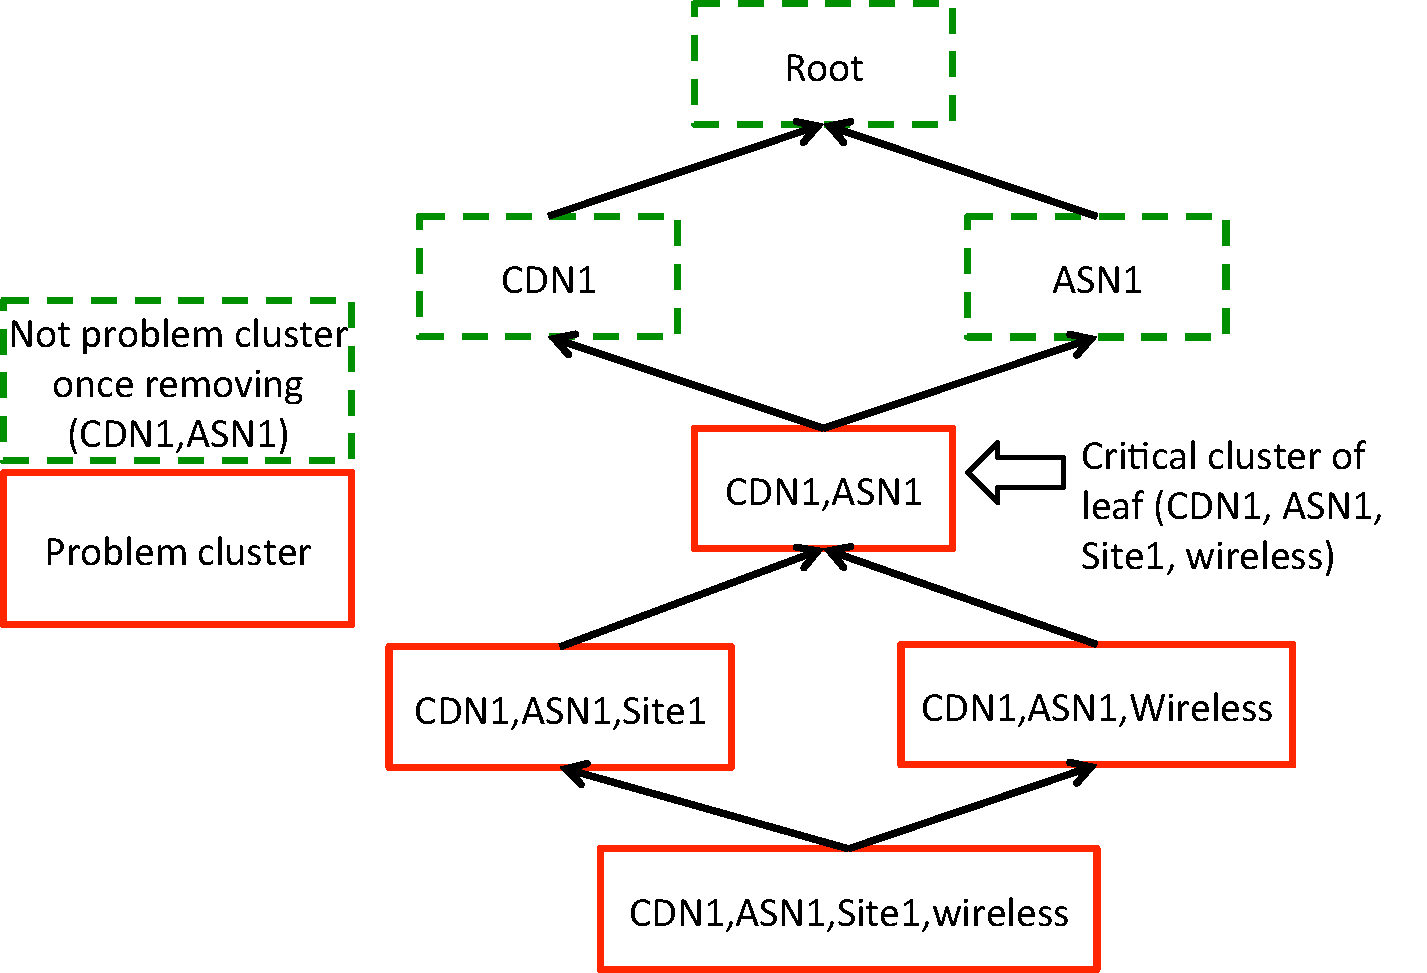
\includegraphics[width=0.7\textwidth]{figures/conext13-criticalcluster_example.pdf}
%\vspace{-0.3cm}
\caption{An illustration of the phase transition idea for  identifying a \criticalcluster. 
%Intuitively,  removing any one feature from this \criticalcluster will cease to 
%be a \problemcluster and adding any feature  to it will continue to be a \problemcluster.
}
\label{fig:method:critclustr2}
\end{figure} 

\subsection{Temporal Patterns}
\label{subsec:measurement:video:temporal}

We begin by analyzing the temporal \emph{prevalence} and 
\emph{persistence} of the \problemclusters.

\mypara{Prevalence of \problemcluster} 
We define the \emph{prevalence} of a \problemcluster as the 
fraction of the total number of epochs in which this cluster 
appears as a \problemcluster.  
% Consider the example in Figure~\ref{fig:method:temporal} with a
%total of 6 epochs, the prevalence of the cluster ``$ASN1$, $CDN1$'' is
%$\frac{4}{6} = 0.67$ and similarly the prevalence of the cluster ``$CDN2$'' is
%$\frac{5}{6} = 0.83$.  
Figure~\ref{fig:measure:prevalence} shows the distribution of 
the prevalence of the \problemclusters for the different
quality metrics. We see a consistent pattern  across all quality 
metrics that around 10\% of the clusters have a prevalence 
greater than 8\% across all metrics. 
In other words, many of these \problemclusters are repeated 
observations that are recurrent problem events. 

\mypara{Prevalence of \problemcluster}
We define the \emph{persistence} of a \problemcluster in terms 
of the length of the consecutive occurrences of this cluster as a
\problemcluster.  
To this end, we coalesce consecutive occurrences of the cluster 
into a single logical event that lasts for multiple hours. 
For each \problemcluster, we  consider the distribution of the 
length of these ``streaks'' and report the median value.
%\emph{median}  and the \emph{maximum}  value. 
%For the timeseries in Figure~\ref{fig:method:temporal}, the ``$ASN1$,$CDN1$'' cluster
%has a median and maximum persistence of 2 while the ``$ASN2$'' cluster has a
%maximum persistence of 4. (In this simple series, the median and max coincide,
%but more generally they will not.)
Figure~\ref{subfig:measure:persistence-median} shows 
the distribution of the median persistence. 
For three of the metrics, more than 60\% of the \problemclusters 
have a median duration that last more than 2 hours.



\begin{figure*}[t]
\centering
\hspace{-1.5cm}
\captionsetup[subfigure]{justification=centering,farskip=-1pt,captionskip=5pt}
\subfloat[Distribution of the prevalence of  \problemclusters]{
   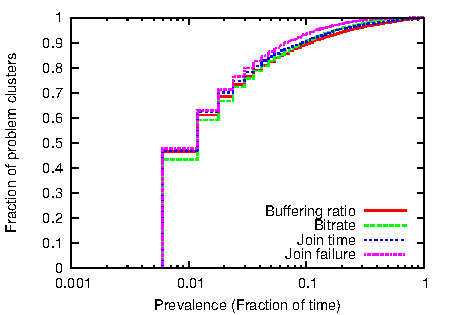
\includegraphics[width=0.52\textwidth] {figures/conext13-figure-cdf-sc-prevalence.pdf}
   \label{fig:measure:prevalence}
 }
\hspace{-0.5cm}
\subfloat[Inverse CDF of the median persistence of \problemclusters]{
   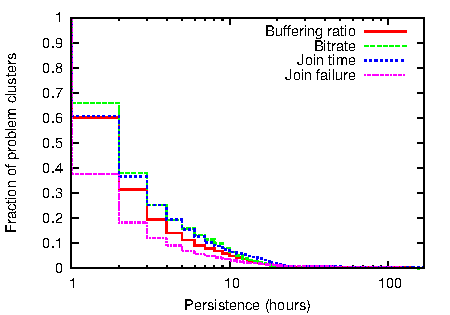
\includegraphics[width=0.52\textwidth] {figures/conext13-figure-cdf-sc-persistence-median.pdf}
   \label{subfig:measure:persistence-median}
 }
 \hspace{-1.5cm}
\caption{Distributions of the prevalence and persistence of  \problemclusters.
We find a natural skewed distribution with a few 
 clusters having high prevalence. 
 Many \problemclusters last multiple hours and that a non-trivial 
 number of \problemclusters last for tens of hours.}
\label{fig:}
\end{figure*}

\subsection{Spatial Patterns}
\label{subsec:measurement:video:spatial}

The previous results showed that there are a non-trivial 
number of persistent/prevalent \problemclusters that last for
several hours. 
As we discussed earlier,  multiple \problemclusters may 
be implicitly related by a single root cause as we saw in
Figure~\ref{fig:method:critcluster}.  
To this end, we focus next on the \criticalclusters using the 
algorithm described in 
Section~\ref{subsec:measurement:video:method}. 
Recall that every  \criticalclusters is also a \problemcluster; 
i.e.,  it has a sufficiently high problem ratio and it has a 
significant number of sessions. The motivation to focus on 
a few critical cluster rather than all \problemclusters is the 
observation (as shown shortly) that a small fraction of 
\problemclusters cover most of the \problemsessions.

\begin{figure}[t]
\centering
   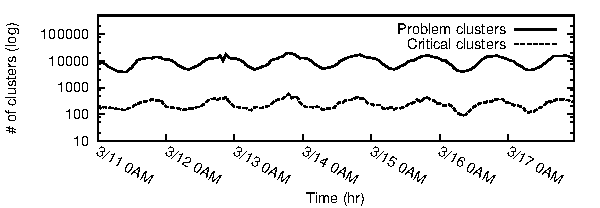
\includegraphics[width=0.7\textwidth] {figures/conext13-time-cluster-count-join-time.pdf}
%\vspace{-0.3cm}
\caption{The number of \criticalclusters is significantly  
smaller than the number of \problemclusters. 
The timeseries shown here  is for the join time; we see 
similar  results for the other quality metrics too.}
\label{fig:critical:reduction}
\end{figure}


\mypara{Critical cluster analysis}
Figure~\ref{fig:critical:reduction} shows the number of 
\problemclusters relative to the number of \criticalclusters 
in the case of the Join Time metric. 
We see that  number of \criticalclusters is almost 
50$\times$ lower than the number of \problemclusters 
suggesting that there are indeed a small number of 
events that might have ``caused''  most  problems.  
One natural question is whether  the \criticalclusters 
\emph{cover} most of the \problemsessions. 
Table~\ref{tab:critical:reduction} summarizes the mean 
coverage and reduction  of the \criticalclusters for the four 
quality metrics and in all cases, we see that the number of 
\criticalclusters is only   2-3\% of the number of 
\problemclusters (i.e., 50$\times$ fewer), but they manage to
cover 44--84\% of the \problemsessions. 
As a point of reference,  we also show the coverage of 
the \problemclusters; i.e., not  all sessions are part of a 
\problemcluster as they may be part of  small clusters or 
clusters with very small \problemratio. 
We see that the \criticalclusters cover almost all 
\problemsessions that are part of some \problemcluster; 
i.e., many of the coverage  gaps are really due to 
\problemsessions that belong to a statistically insignificant 
cluster (i.e., either with too few sessions or with 
too few \problemsessions).
 
 
\begin{table}[t]
\begin{center}
\begin{small}
\begin{tabular}{c|p{2cm}|p{2cm}|p{2.5cm}|p{2.5cm}}
Metric	& Mean \problemclusters & Mean \criticalclusters & Mean \problemcluster coverage & Mean \criticalcluster coverage\\ \hline 
BufRatio	 & 10433 & 286 (2\%) & 0.8 & 0.66 (82\%) \\
JoinTime & 9953 & 247 (2\%) & 0.86 & 0.83 (96\%) \\
JoinFailure & 9620 & 302 (3\%) & 0.87 & 0.84 (96\%)\\
Bitrate & 9437 & 287 (3\%) & 0.57 & 0.44 (77\%)
\end{tabular}
\end{small}
\end{center}
\caption{Reduction via focusing only on \criticalclusters 
and the effective coverage  of the \criticalclusters.}
\label{tab:critical:reduction}
\end{table}


Next, we analyze the structure of the \criticalclusters for 
the different quality metrics. 
First, we analyze the types of  client/session  feature 
combinations that appear frequently in the \criticalclusters. 
Then, we analyze if the different metrics are correlated in the 
\criticalclusters. Finally, we highlight some interesting 
observations  and some hypothesis to explain  
the most prevalent \criticalclusters. 



%\begin{figure}[t]
%\centering
%\captionsetup[subfigure]{justification=centering,farskip=-1pt,captionskip=5pt}
%\subfloat[BufferingRatio]{\label{subfig:measure:pie-bufferingratio}
%   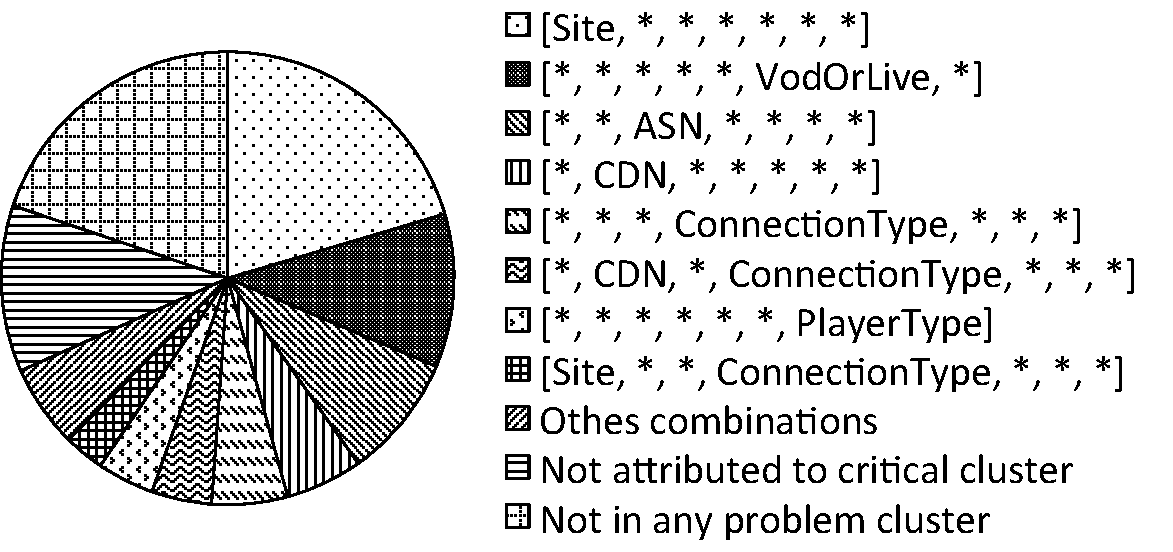
\includegraphics[width=0.48\textwidth] {figures/conext13-figure-pie-bufferingratio.pdf}
% }
%\subfloat[Bitrate]{\label{subfig:measure:pie-bitrate}
%   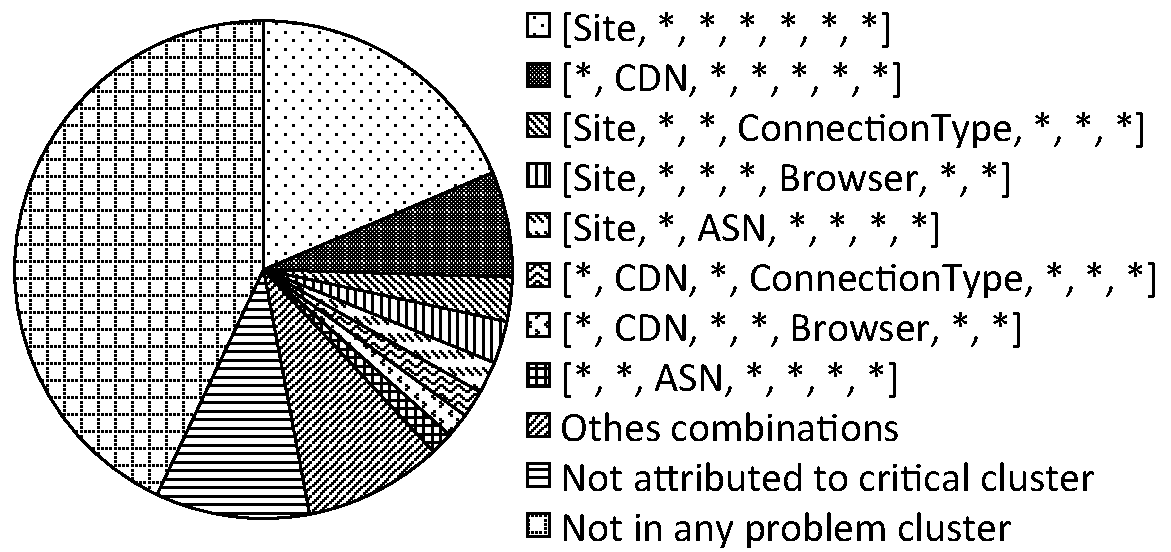
\includegraphics[width=0.48\textwidth] {figures/conext13-figure-pie-bitrate.pdf}
% }\\
%\subfloat[JoinTime]{\label{subfig:measure:pie-jointime}
%   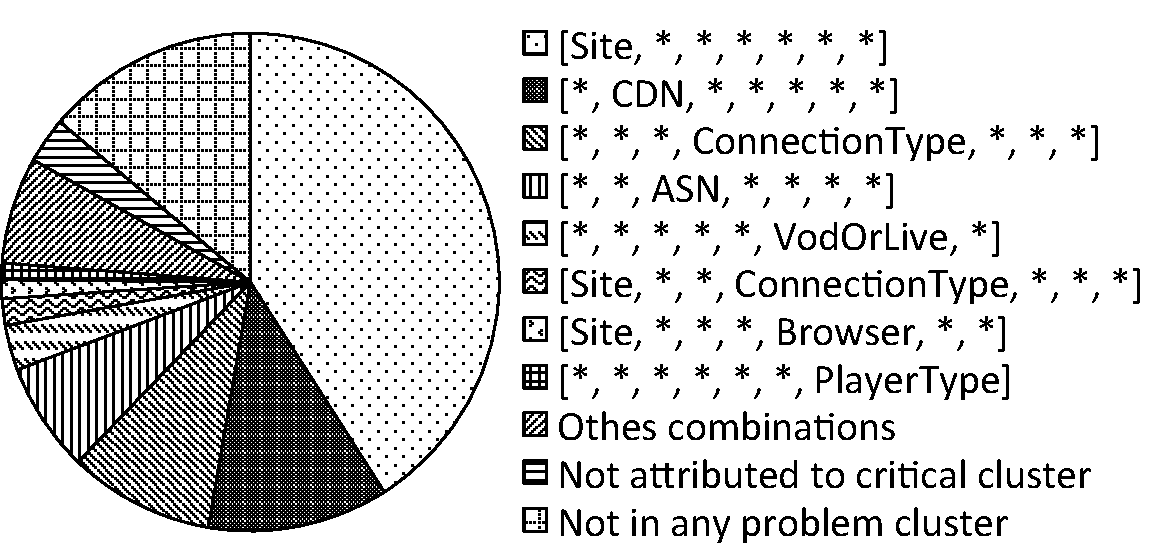
\includegraphics[width=0.48\textwidth] {figures/conext13-figure-pie-jointime.pdf}
% }
%\subfloat[JoinFailure]{\label{subfig:measure:pie-joinfailure}
%   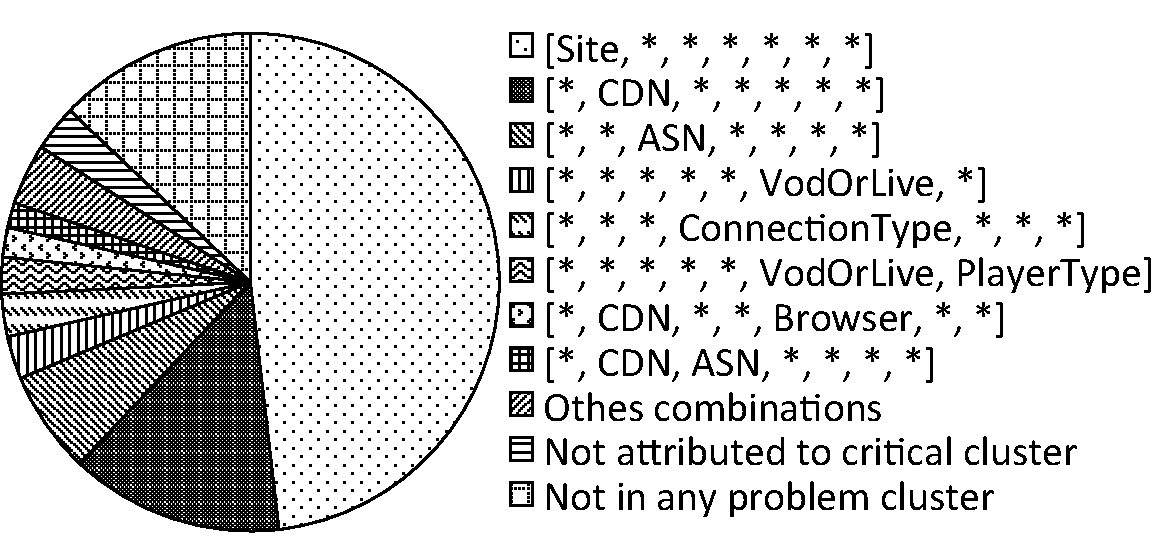
\includegraphics[width=0.48\textwidth] {figures/conext13-figure-pie-joinfailure.pdf}
% }
%\caption{Analyzing the structure of the \criticalclusters.
%The result show a breakdown of the total number of 
%sessions attributed to a specific type of \criticalcluster. 
%Note that there may be multiple values of these features;
%i.e., there can be many Sites and many CDNs  contributing 
%to the Site and CDN sector.}
%\label{fig:critical:pie}
%\end{figure}
%
%\mypara{Types of clusters} 
%Figure~\ref{fig:critical:pie} shows a breakdown of the 
%types of \criticalclusters  for different quality metrics.  
%We aggregate \criticalclusters into the different feature 
%dimension(s) they represent. 
%For instance, if we see a \criticalcluster for $CDN1$ and 
%$CDN2$, we count these toward the CDN contribution 
%in the pie chart.   
%Some \problemsessions may remain unaccounted for 
%in this breakdown for two reasons:
%(a) they are not part of a significant enough 
%\problemcluster or 
%(b) our algorithm did not assign a \criticalcluster for a 
%\problemcluster. 
%This mirrors   the coverage observation we saw earlier in 
%Figure~\ref{fig:critical:reduction}
% and  Table~\ref{tab:critical:reduction}. 
%In almost all cases, most of the unaccounted for sessions 
%fall outside any \problemcluster;  i.e., this is not due to 
%the \criticalcluster detection algorithm. 
%The result shows that the most dominant category of 
%\criticalclusters actually corresponds to a
%\emph{content provider} (labeled as ``Site'').  
%We also see that CDN, ASN, and ConnectionType are
% also prominent types of \criticalclusters across all 
% quality metrics. 
%This suggests that most quality issues are potentially 
%caused by server-side (Site or CDN) or client-side 
%(ASN, ConnectionType) problems rather than a 
%combination (which indicates a bad path between 
%client and server) or other features.

%This is
%related to the coverage observation we saw earlier---with the exception of the
%bitrate category, the coverage is quite high.
 
%Note that this does not mean that the same set of \criticalclusters appear
%across all metrics as we will see next.


\mypara{Understanding most prevalent  \criticalclusters} 
In order to illustrate the causes for the problem,  we 
consider the \criticalclusters with a prevalence higher 
than 60\% for the different quality metrics. 
For clarity of presentation, we only consider the 
\criticalclusters whose features fall in one of the following 
categories: ASN, CDN, Site, and ConnectionType as
our previous breakdown shows these as the most 
dominant features.  
We present this analysis with two disclaimers.  
First, due to the sensitive nature of this data, we do not 
present the names of the actual providers, but focus on their
characteristics.  
Second, this involves a fair amount of manual analysis and
domain knowledge. As such, we intend this result to be 
illustrative (and somewhat speculative) rather than attempt 
to be conclusive.  
This said, we still believe that the high-level insights are 
still useful to inform future video delivery architectures.

Table~\ref{tab:depth} presents some of the anecdotal 
examples we observed.  
The empty cells simply indicate that there were no 
\criticalclusters in this category with a prevalence higher 
than 60\%. 
We see a few interesting patterns here.  
In terms of buffering ratio, we see that the top ASNs are 
typically in Asia, and the content providers that had issues 
typically only had a single bitrate of content. 
The CDNs with buffering/join time problems are also
typically ``in-house'' CDNs run by the Site itself; i.e., 
not a third-party CDN like Akamai or Limelight.  
We also see that wireless connections and wireless
ISPs appear in the buffering and bitrate cells 
respectively, which is somewhat expected. 


One interesting artifact we uncovered in the case of 
join time was that these were mostly ASNs in China 
accessing content from Chinese CDNs but there were
third-party player modules loaded from US providers 
that led to higher join times. Another curious 
observation is that all the Sites with significant join
failures tended to use the same global CDN. 
However, the CDN in aggregate does not have a 
significant presence in terms of failures, except in the 
case of these Sites.\footnote{These Sites used a single 
CDN; recall that our \criticalcluster algorithm will 
prefer more compact descriptions and thus
features these problems to the Site rather than the 
single Site-CDN combination.} 
We speculate that these, presumably low-end, 
providers may have lower priority service and could 
have potentially benefited from using multiple CDNs.


\begin{table}[t]
\begin{center}
\begin{small}
\begin{tabular}{p{1.5cm}|p{3.5cm}|p{2.5cm}|p{3.5cm}|p{2.5cm}}
		& ASN &  CDN   & Site  & ConnType  \\ \hline 

BufRatio	 & Asian ISPs  & In-house, single bitrate   & Single bitrate &  Mobile wireless  \\   \hline
JoinTime 	&  Chinese ISPs accessing CDNs in China, but player loads modules from US CDN	& In-house CDNs of UGC providers & High bitrates  \\  \hline 
JoinFailure 	&   & Same set as buffering ratio & Same single global CDN, maybe low priority providers &  \\ \hline 
Bitrate 	& Wireless provider &   & UGC Sites &    
\end{tabular}
\end{small}
\end{center}
\caption{Analysis of the most  prevalent \criticalclusters. 
A empty cell implies that we found no interesting 
 cluster in this combination.}
\label{tab:depth}
\end{table}


\subsection{Cross-Metric Correlations} 
\label{subsec:measurement:video:correlation}

%We saw in the previous  graph that the types of
% \criticalclusters that contribute the most 
% \problemsessions are very similar across different 
%quality metrics.  
%Note, however, that this does not necessarily mean 
%that the actual set of \criticalclusters are identical. 
%In other words, a different set of CDNs or Sites may 
%be responsible for problems across buffering ratio and
%join time. 
Next, we would like to know how much the \criticalclusters
of different quality metrics correlate with each other.
In other words, a different set of CDNs or Sites may 
be responsible for problems across buffering ratio and
join time. 
To analyze this, we compute the \emph{Jaccard similarity} 
index between the top-100 in terms of the total number 
of \problemsessions covered  \criticalclusters  
for the different metrics. 
(The Jaccard similarity measure for two sets A and B 
is $\frac{|A \cap B|}{|A \cup B|}$.)
We find that the overlap between the different 
metrics is only around 23\% in the best case (buffering 
ratio and join time) and in the worst case is only around
1\% (between bitrate and join failure).  
We manually analyzed the specific clusters and we 
found that  the actual set of Site, CDN, and ASN
\criticalclusters are indeed very different.  

%We look at this in more depth next.
 


%\begin{table}[t]
%\begin{center}
%\begin{small}
%\begin{tabular}{c|c|c|c|c}
%		& Buffering Ratio & Join Time & Join failure & Bitrate \\ \hline 
%Buffering Ratio	 & \fillme & 0.22 & 0.13 & 0.07 \\
%Join Time & \fillme & \fillme & 0.09 & 0.08 \\
%Join failure & \fillme & \fillme & \fillme & 0.008 \\
%Bitrate & \fillme & \fillme & \fillme & \fillme 
%\end{tabular}
%\end{small}
%\end{center}
%\tightcaption{Average Jaccard similarity index between the top-\fillme \criticalclusters for the different metrics. 
% We see that most metrics are relatively uncorrelated, possibly because the 
% critical features are very different.}
%\end{table}

\begin{table}[t]
\begin{center}
\begin{small}
\begin{tabular}{p{2cm}|p{2cm}|p{2cm}|p{2cm}|p{2cm}|p{2cm}}
	BufRatio vs. Bitrate & BufRatio vs. JoinTime & BufRatio vs. JoinFailure & Bitrate vs. JoinTime & Bitrate vs. JoinFailure & JoinTime vs. JoinFailure\\ \hline 
0.07 & 0.23 & 0.13 & 0.08 & 0.01 & 0.09 \\
\end{tabular}
\end{small}
\end{center}
\caption{Average Jaccard similarity index between the top 
100 \criticalclusters for the different metrics. 
 We see that most metrics are relatively uncorrelated, possibly because the 
 critical features are very different.}
\end{table}


\subsection{Key Observations}
\label{subsec:measurement:video:discuss}
%\subsection{Key Observations}

Our key observations from the analysis of \problemclusters 
and  \criticalclusters  are:  

\begin{packeditemize}

\item There is a distinct skewed distribution  in the prevalence; 
around 8-12\% of the \problemclusters appear more than 
10\% of the time.

\item There is also a skewed distribution  in the persistence; 
more than 60\% of  \problemclusters have a median duration 
greater than 2 hours.  

\item We find that a small number of \criticalclusters 
(2-3\% of the number of \problemclusters) can account 
for 44-84\% of all \problemsessions. 

\item While the set of feature combinations in the 
\criticalclusters that cover the most number of 
\problemsessions is very similar across the quality
metrics (i.e., Site, CDN, ASN), the actual values of 
these features is very different (with a max overlap of 23\%). 

\item  We see a few expected patterns  such as Asian 
and wireless ISPs appearing  as most prevalent \criticalclusters. 
We  see some unexpected patterns that can be easily alleviated 
(e.g., the player modules loaded remotely for Chinese users) 
and Sites that could benefit from standard strategies such as 
using more fine-grained bitrates or using multiple CDNs.

\end{packeditemize}





\section{Internet Telephony}
\label{sec:measurement:voip}

We have seen in 
Section~\ref{subsec:related:voip-qoe} that user 
experience is sensitive to poor network performance 
and that a significant fraction of calls suffer from poor 
performance when using \direct routing. 

In this section, we use production data from a large VoIP service 
provide \skype (same dataset described in
 Section~\ref{subsec:related:voip-qoe}) 
to understand the QoE problems in Internet telephony
based on a similar spatial and temporal analysis used in the last section.
We begin by describing the dataset, QoE metrics, and the methodology
of analyzing spatial and temporal patterns
of VoIP QoE problems (Section~\ref{subsec:measurement:voip:method}),
and present our results in 
Section~\ref{subsec:measurement:voip:spatial}, 
~\ref{subsec:measurement:voip:temporal}, and
~\ref{subsec:measurement:voip:correlation}.
%and finally discuss the key takeaways in 
%Section~\ref{subsec:measurement:voip:discuss}
%quantify the impact of network metrics on 
%audio call quality, and patterns of poor network performance. 
%The observations motivate the need for and the design 
%requirements of \hybrid.


%{\em How well does PNR on average values compare to 
%using full packet traces?} 
%Analysis of a subset of ($70$K) calls with full packet traces 
%shows that $80\%$ of calls rated ``non-poor'' using the 
%thresholds on average metrics (``at least one poor metric'') 
%have a (packet-trace based) MOS score higher than 
%three-quarters ($75\%$) of calls rated ``poor'' using the 
%average metrics. We run a proprietary MOS calculator 
%on the packet traces that contain send/receive timestamps 
%for each packet and loss information. 
%This shows that defining the thresholds on average values 
%of the call is a reasonable approximation.

\subsection{Methodology}
\label{subsec:measurement:voip:method}

\mypara{Identifying bad QoE}
First, we define bad VoIP QoE by a similar threshold-based method
as we defined problem sessions in video.
We define the {\em poor network rate} (PNR) of a network 
metric for a set of calls as the fraction of calls whose performance 
on the metric is worse than the chosen thresholds: 
RTT $\geq 320$ms, loss rate $\geq 1.2\%$, jitter $\geq 12$ms. 
Recall from Figure~\ref{fig:perf-cdf} that these thresholds 
correspond to the user-specified poor call rate (PCR) of $0.3$.
These values are in line with literature from industry 
and standards bodies that recommend one-way end-to-end 
delay of no more than $150$ ms and a packet loss rate of 
no more than $1\%$ for good call quality~\cite{cisco-voip, itu}. 

\mypara{Clustering calls}
Similarly to video streaming, we would like to understand whether
the calls with bad network performance concentrate spatially 
(e.g., are they mostly International calls?) and persist
over time. To this end, we group calls in the dataset based on 
different spatial features (e.g., geo-locations and IP prefixes 
of the caller and callee) as well as time-stamp (the date in which
the call was made).


%Next, we analyze whether the calls with poor networks 
%share common patterns. This subsection focuses on 
%{\em spatial} patterns while
%Section~\ref{subsec:measurement:voip:temporal} 
%looks at {\em temporal} patterns.

\subsection{Spatial Patterns}
\label{subsec:measurement:voip:spatial}



% We define the {\em poor network rate} (PNR) for a given set of calls as the fraction of calls whose network performance is worse than the thresholds: RTT $\geq 320$ms, loss rate $\geq 1.2\%$, jitter $\geq 12$ms. PNR can be measured both on the individual metrics (how often were each of them poor?) as well as collectively (how often was {\em at least one} of the metrics poor?). Recall from Figure~\ref{fig:perf-cdf} that these thresholds correspond to the user-specified poor call rate (PCR) of $0.3$.
% to poor call performance with a probability of $0.5$. 

\begin{figure}[t!]
\centering
\subfloat[\small{International vs. domestic}]
{
        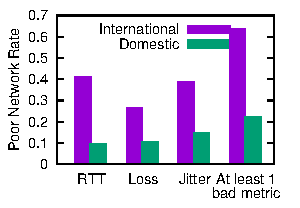
\includegraphics[width=0.45\textwidth]{figures/Via-Opportunity-International.pdf}
        \label{subfig:opportunity-international}
}
\subfloat[\small{Countries of one side of a call}]
{
        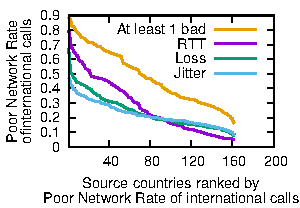
\includegraphics[width=0.45\textwidth]{figures/Via-Opportunity-International-ByCountry.pdf}
        \label{subfig:international-bycountry}
}
\caption{International vs. Domestic Calls.}
\label{fig:country}
\end{figure}

\mypara{International vs. domestic calls} 
On all three network metrics, we see that international 
calls (between users in different countries) have a
 higher PNR, i.e., they are more likely to suffer from 
 bad network performance than domestic calls. 
Figure~\ref{fig:country} shows a $2-3\times$ higher 
PNR on international calls than on domestic calls. 
The figures also show the fraction of calls with at least 
one metric being poor (the last pair of bars), where the 
gap between international and domestic calls is even 
larger. 
Though conclusively diagnosing the root cause of bad 
performance on international calls is hard and beyond 
the scope of this work, the higher PNR for international 
calls points to the WAN path as the culprit.\footnote{One 
aspect is that users tend to use VoIP 
regardless of its performance for international calls, 
unlike domestic calls.} %\cmrvnp{we speculate that it is because ISPs have less incentive to ensure good quality for international calls than domestic ones.}}

% \vnp{The "at least 1 bad metric" bars seem at least as tall as the other bars stacked up, which suggests that there is little overlap between the subsets for which each metric is poor.}

To understand this further, 
Figure~\ref{subfig:international-bycountry} zooms into 
the international calls and classifies them by the country 
of the callers (source). 
We see that there is a skewed distribution, with certain 
countries having a PNR as high as on the individual metrics. 
The PNR of international calls across the remaining 
countries drops gradually but half of them still see a 
non-negligible PNR of $25\%-50\%$. 
This suggests that poor network performance is 
quite widespread, highlighting the suitability of a 
{\em globally} deployed overlay network that provides 
high performance inter-connection between overlay nodes.
% and calling for a selective approach to routing via the managed network. 
% but the overall distribution is flat, indicating that most countries do not have particularly poor network performance. 

\begin{figure}[t!]
\centering
%\hspace{-0.5cm}
\subfloat[Inter-domain vs. intra-domain]
{
        \includegraphics[width=0.45\textwidth]{figures/Via-Opportunity-Interdomain.pdf}
        \label{subfig:opportunity-interdomain}
}%\hspace{-0.5cm}
\subfloat[Source AS]
{
        \includegraphics[width=0.45\textwidth]{figures/Via-Opportunity-Interdomain-ByAs.pdf}
        \label{subfig:interdomain-byas}
}%\hspace{-0.5cm}
\caption{Inter-domain vs. intra-domain calls.}
\label{fig:domain}
\end{figure}

\mypara{Inter-AS vs. intra-AS calls} % The above trends persist when we splice calls by the AS domains of the source and destinations. 
Similar to international calls, calls across ASes 
are $2-3\times$ more likely to experience poor 
network performance than those within the same 
AS domain. %Also, while calls originating from a small fraction of the ASes have a much higher PNR, the overall distribution is even. 
%This, again, points to the need for a selective approach to routing via the global managed overlay.
This, again, points to the need for enabling alternatives to default routing to improve WAN performance.
% a relay system that provides wide-area routing of better performance.

\begin{figure}[t!]
\centering
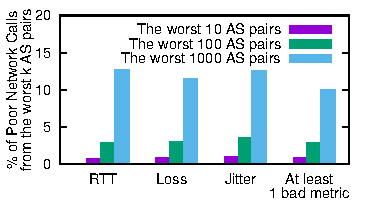
\includegraphics[width=0.6\textwidth]{figures/Via-BadContribution-Top-AsPair.pdf}
\caption{The percentage of calls over poor network 
conditions that come from the worst $n$ AS pairs; 
AS-pairs are ranked in descending order of their 
contribution to total amount of calls with poor performance.}
 %\ga{Change ``top'' to ``worst''.}
\label{fig:bad-contribution}
\end{figure}

\mypara{Not just a few problematic source-destination pairs}
Contrary to our expectation, a few source-destination pairs 
alone do {\em not} account for a big chunk of the PNR. % Our hypothesis was to observe the commonly occurring ``Pareto'' effect.
 Figure~\ref{fig:bad-contribution} shows the fraction of 
 calls that suffer from poor network performance from the 
 worst AS pairs, ranked in order of their contribution to the 
 overall PNR. %Across different metrics, we see that the calls with poor network metrics are not limited to a handful of AS pairs. 
Even the worst $1000$ AS pairs together only count for less 
than $15\%$ of the overall PNR. %\vnp{I'm unable to reconcile these numbers with the bars depicted in Fig 5.} 
This means that localized solutions that fix a few bad ASes 
or AS pairs, e.g., informing the AS administrators or the 
clients directly regarding their ISPs, are not sufficient. 
 
%\vnp{Absolute counts don't quite tell the full story. We should also report what fraction of all AS pairs seen is represented by k}
 
While the above analysis was at the granularity of ASes, 
we also tested at other, finer granularities (e.g., $/24$ and 
$/20$ prefixes of the caller and callee IP addresses) and 
found similar results (of not just a few culprits).
In fact, for the pairs with sufficient data density at the $/24$ 
granularity, we found that performance distributions of the 
network metrics were similar to those at the granularity of ASes.% are close to those at the granularity of $/24$; for instance, on more than 85\% $/24$ pairs where we have at least 10 calls, the average RTT is within 50\% away from that of the corresponding AS pairs.



\begin{figure}[t!]
\centering
%\subfigure[Timeseries\jc{Needs to be changed}]
%{
%        \includegraphics[width=0.45\textwidth]{new-figs/Timeseries-badrate.pdf}
%        \label{subfig:temporal-structure-timeseries}
%}
\subfloat[\small{Persistence}]
{
        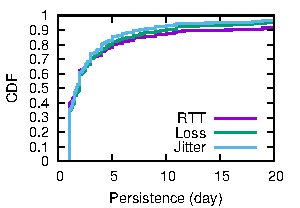
\includegraphics[width=0.45\textwidth]{figures/Via-Persistence-AsPair.pdf}
        \label{subfig:temporal-structure-persistence}
}
\subfloat[\small{Prevalence}]
{
        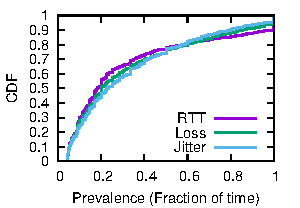
\includegraphics[width=0.45\textwidth]{figures/Via-Prevalence-AsPair.pdf}
        \label{subfig:temporal-structure-prevalence}
}
\caption{Temporal patterns of poor network performance. 
Figure~\ref{subfig:temporal-structure-persistence} and 
\ref{subfig:temporal-structure-prevalence} show the distribution of 
the persistence and prevalence of AS pairs having high PNR.}
\label{fig:temporal-structure}
\end{figure}





\subsection{Temporal Patterns}
\label{subsec:measurement:voip:temporal}

We now analyze temporal patterns of poor network 
performance. 
We perform this analysis by grouping the 
performance of AS pairs into $24$-hour time 
windows.\footnote{Different grouping granularities
yielded similar observations.}
We conservatively label an AS pair as having 
{\em high PNR} for a specific metric (on a given day) if 
its PNR on that day is at least $50\%$ higher than the 
overall PNR of all calls on that day. 

%Knowing what types of calls are more likely to have poor performance, however, does not mean they can be easily fixed. Next, we study the spatial and temporal patterns of bad network performance, and show that fixing a handful of AS pairs in specific time periods does not address most of them, which suggests the needs for a system that can adaptively alleviate bad network performance for users all over the world.

%\myparatight{Methodology} To understand the spatial and temporal patterns of bad network performance, we consider the performance distribution of each AS pair within different time windows of 24 hours. We first group the calls based on the pair of source and destination AS, and to ensure statisical significance, we consider each AS pair that have at least 20 calls in each day\footnote{We decide to group calls by source and destination AS pair on a daily base because it is the finest granularity that still have enough calls for most of the time. We used different grouping granularities and found qualitatively similar observations.}. 
%\ga{Let's see if we can argue for AS-level analysis as reasonable. Maybe present some /24 granularity data, show that the trends are similar when there is sufficient data, and say we will use AS-level data owing to the density? As we have all discussed before, it is not a natural granularity to pick unless we say why so.}

Figure~\ref{subfig:temporal-structure-persistence} and 
\ref{subfig:temporal-structure-prevalence} show the 
distribution of {\em persistence} and {\em prevalence} of 
high PNR AS-pairs. 
The {\em persistence} of an AS pair is the median 
number of consecutive days when it has high PNR. 
The {\em prevalence} of an AS pair is the fraction of 
time it has high PNR.
The figures show a highly skewed distribution with 
$10\%-20\%$ AS pairs always having high PNR, while 
$60\%-70\%$ AS pairs have poor performance for less 
than $30\%$ of time and lasting no longer than one 
day at a stretch. 
%These majority of AS pairs whose poor network performance is neither prevalent nor persistent should be improved in a dynamic manner.
%This means the poor performance of most AS pairs is neither prevalent nor persistent.
%This means that to fix the majority of AS pairs that are neither prevalent nor persistent that statically configuring a solution to improve only the (relatively few) most prevalent and persistent AS pairs is not sufficient; 
This observation suggests that instead of statically 
configuring the system to improve performance for 
only the (relatively few) most prevalent and persistent 
AS pairs, we need to dynamically decide if a call 
should use default Internet routing or be relayed. % sent through overlays.
%It reinforces the point 
%, in order to improve performance for the majority of AS pairs. 


\subsection{Cross-Metric Correlations}
\label{subsec:measurement:voip:correlation}

As there could be dependencies between network 
metrics, improving one metric may increase PNR of another 
metric. 
Figure~\ref{fig:perf-correlation} shows the three pair-wise 
correlations. 
While the plot is based on an aggregation of data across all 
calls and paths, the substantial spread suggests at least the 
possibility that improving one performance metric {\em could} 
lead to a worsening of the other metrics. 
Therefore, we also focus on reducing PNR of three metrics 
collectively, i.e., minimizing how often {\em at least one} of 
the metrics is poor.

\begin{figure}[t!]
\centering
\subfloat[\small{RTT vs. loss rate}]
{
        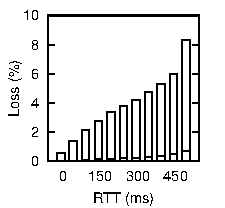
\includegraphics[width=0.3\textwidth]{figures/Via-Quality-Correlation-RTT-loss.pdf}
        \label{subfig:}
}
\subfloat[\small{RTT vs. jitter}]
{
        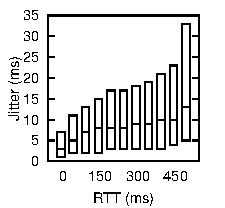
\includegraphics[width=0.3\textwidth]{figures/Via-Quality-Correlation-RTT-jitter.pdf}
        \label{subfig:}
}
\subfloat[\small{Jitter vs. loss rate}]
{
        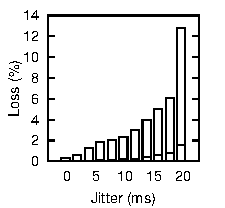
\includegraphics[width=0.3\textwidth]{figures/Via-Quality-Correlation-jitter-loss.pdf}
        \label{subfig:}
}
\caption{Pair-wise correlation between performance metrics. 
The Y-axis shows the distribution ($10^{\text{th}}$, $50^{\text{th}}$, 
$90^{\text{th}}$ percentiles) of one metric as a function the other 
metric over the same set of calls.}
%\ga{Only 25th, median, 90th? Also jitter vs. loss}
\label{fig:perf-correlation}
\end{figure}




%\subsection{Discussion}
%%\subsection{Key Observations}
%\label{subsec:measurement:voip:discuss}
%
%The key observations from this section are:
%\begin{enumerate}
%\item {\em Network performance matters.} User experience of 
%calls is impacted by even small changes in network metrics. 
%\item {\em Wide-area} communication, such as international 
%and inter-domain calls, are more prone to bad network performance, 
%and have a large room of improvement.
%\item Calls suffering from poor networks are spread {\em spatially} 
%(across ASes) and {\em temporally}. 
%%Most calls with poor network performance are not from a handful of source-destination AS pairs. And most source-destination pairs only experience high PNR for a relatively short period of time.
%\end{enumerate}

%These observations motivate the need for a network overlay (Observation 1) that provides better paths with a {\em global} footprint of overlay nodes (Observation 2), and the need to choose routes {\em selectively} and {\em dynamically} (Observation 3). 





\section{Summary}
\label{sec:measurement:summary}

In this chapter, we have used empirical studies based on real large-scale datasets 
of video and VoIP QoE to shed light on the structures of QoE problems in the wild.
Our findings suggest that there are persistent critical structures in the factors that 
determine video and VoIP QoE. Our key observations can be summarized as follows:

\begin{itemize}

\item {\em QoE depends on critical spatial structures.}
Most quality problems can be attributed to a relatively small number of feature value
combinations. We observe that in both Internet video and Internet telephony, bad 
quality can be attributed to smaller number of session-level features. For instance,
we see that \criticalclusters of bad video quality only account for 2-3\% of all 
\problemclusters. Note that VoIP quality problems are relatively more spatially spread 
out than video quality problems, because VoIP quality depends on both sides of a call, 
while the video quality more often is determined by the client-side performance.


\item {\em Many quality problems tend to 
persist on timescales of tens of minutes to hours.}
We observe that a substantial fraction of problems
last for multiple hours (even days).
For instance, 60\% of the problem clusters have a median
duration that last more than 2 hours.
At the same time, we note that both video and VoIP quality problems 
have highly skewed distributions in the prevalence 
and persistence, where some problems are still transit.


%\item {\em Quality today is not idea.} 
%Across multiple application providers, we observe 
%that a substantial fraction of sessions have bad quality. 
%For instance, 5\% video sessions have a
%buffering ratio larger than 10\%, and 15-17\% Skype
%calls have bad network performance in at least one
%of long latency, high packet loss, or high latency jitter.
%
%\item {\em Most quality problems can be attributed to 
%a relatively small amount of persistent patterns.}
%We observe that in both Internet video and Internet
%telephony, bad quality can be attributed to some
%session-level features (e.g., critical clusters in 
%Section~\ref{subsec:measurement:video:temporal}
%and AS pairs in 
%Section~\ref{subsec:measurement:voip:temporal}).
%These quality problems and features are more stable than 
%fluctuation of quality.

\item {\em Quality problems of different metrics are correlated.} 
Finally, we observed that the quality problems of different metrics are likely 
to be correlated, suggesting that, instead of having to trading one metric for 
another, it is possible to improve multiple metrics simultaneously.

\end{itemize}






\chapter{Predictive QoE Optimization By Critical Feature Analysis}
\label{ch:cfa}

\newcommand{\dda}{{CFA}\xspace}
\newcommand{\system}{{\dda}\xspace}
\newcommand{\ControlPlane}{{global optimization system}\xspace}

In this chapter, we present the first illustration of how \ddn paradigm 
improves video QoE by formulating \ddn as a prediction problem. 
%The goal is 
%to predict video quality  for different choices (e.g., CDN 
%or bitrate) to make optimal decisions.
Prior studies have shown that video quality can be substantially improved
by optimally selecting the best CDN and bitrate for each video session, 
and the key to realize this potential is to build an video quality prediction
system that can accurately predict the quality of a video session, if it were
to use any combination of CDN and bitrate.
%such  {\em data-driven prediction} of 
%video quality can potentially lead to substantial video QoE improvement.
%Many prior efforts have suggested that Internet video 
%QoE  could be dramatically improved by using {\em data-driven 
%prediction} of video quality  for different choices (e.g., CDN 
%or bitrate) to make optimal decisions.
However, building such a prediction system is challenging on two fronts. 
First, the relationships between video quality and observed 
session features can be quite complex. Second, video quality changes 
dynamically. 
Thus, we need a prediction model that is 
(a) expressive enough to capture these complex relationships, 
and (b) capable of updating quality predictions in near 
real-time. 
Unfortunately, several seemingly natural solutions (e.g., 
simple machine learning approaches and simple network models) fail on 
one or more fronts.
%Thus, the potential benefits promised by these prior
%efforts remain unrealized. 

To address these challenges, we present {\em Critical 
Feature Analytics (\dda)}, which is inspired by  the persistent critical 
structures of the QoE-determining factors. 
In particular, video quality is typically determined by a small subset of 
critical features whose criticality persists over several tens of minutes.
This enables a scalable and accurate workflow where 
we automatically learn critical features for different 
sessions on coarse-grained timescales, while updating 
quality predictions in  near real-time. 
Using a  combination of real-world pilot deployment 
and trace-driven analysis, we demonstrate that \dda 
leads to significant improvements in video quality; e.g., 32\% less 
buffering time and 12\% higher bitrate than a random decision maker.

This chapter is organized as follows.
Section~\ref{sec:cfa:background} provides some background on
the promise of video QoE prediction, and identifies key challenges
 in building an accurate video QoE prediction
system.
Then Section~\ref{sec:cfa:outline}, Section~\ref{sec:cfa:design},
and Section~\ref{sec:cfa:impl} outlines the key design ideas 
behind CFA, the detailed design, and implementation of CFA, respectively.
Section~\ref{sec:cfa:eval} presents real-world and trace-driven evaluation that 
demonstrates substantial quality improvement by CFA.
Section~\ref{sec:cfa:insight} uses critical features learned by 
CFA to make interesting
observations about video quality.
Finally, Section~\ref{sec:cfa:discuss} discusses some open issues in 
CFA, Section~\ref{sec:cfa:related} discusses the related work, and 
Section~\ref{sec:cfa:summary} concludes the section.


\section{Background}
\label{sec:cfa:background}

This section begins with some background on video
quality prediction.
 Then, we articulate two key
challenges faced by any video quality prediction system:
(1) The factors affecting video quality are complex, so
we need expressive models; (2) Quality changes
rapidly, so models must be updated in near real-time by
recent quality measurements. We also argue why
existing solutions do not address these challenges.


\subsection{Data-Driven Quality Prediction}
\label{sec:cfa:background:prediction}

Prior work has made the case for a quality optimization 
system (Figure~\ref{fig:globalsystem}) that uses a 
{\em prediction oracle} to suggest the best parameter 
settings (e.g., bitrate, CDN) to optimize quality 
(e.g.,~\cite{sigcomm12,balachandran2013analyzing,
mukerjee2015practical,sigcomm12cdnmulti,c3}).  
Seen in a broader context, this predictive approach 
can be applied beyond Internet video
(e.g.,~\cite{aggarwal2014prometheus,
sambasivan2011diagnosing,
choffnes2010crowdsourcing, velox-cidr,
spand}).

\begin{figure}[t]
\centering
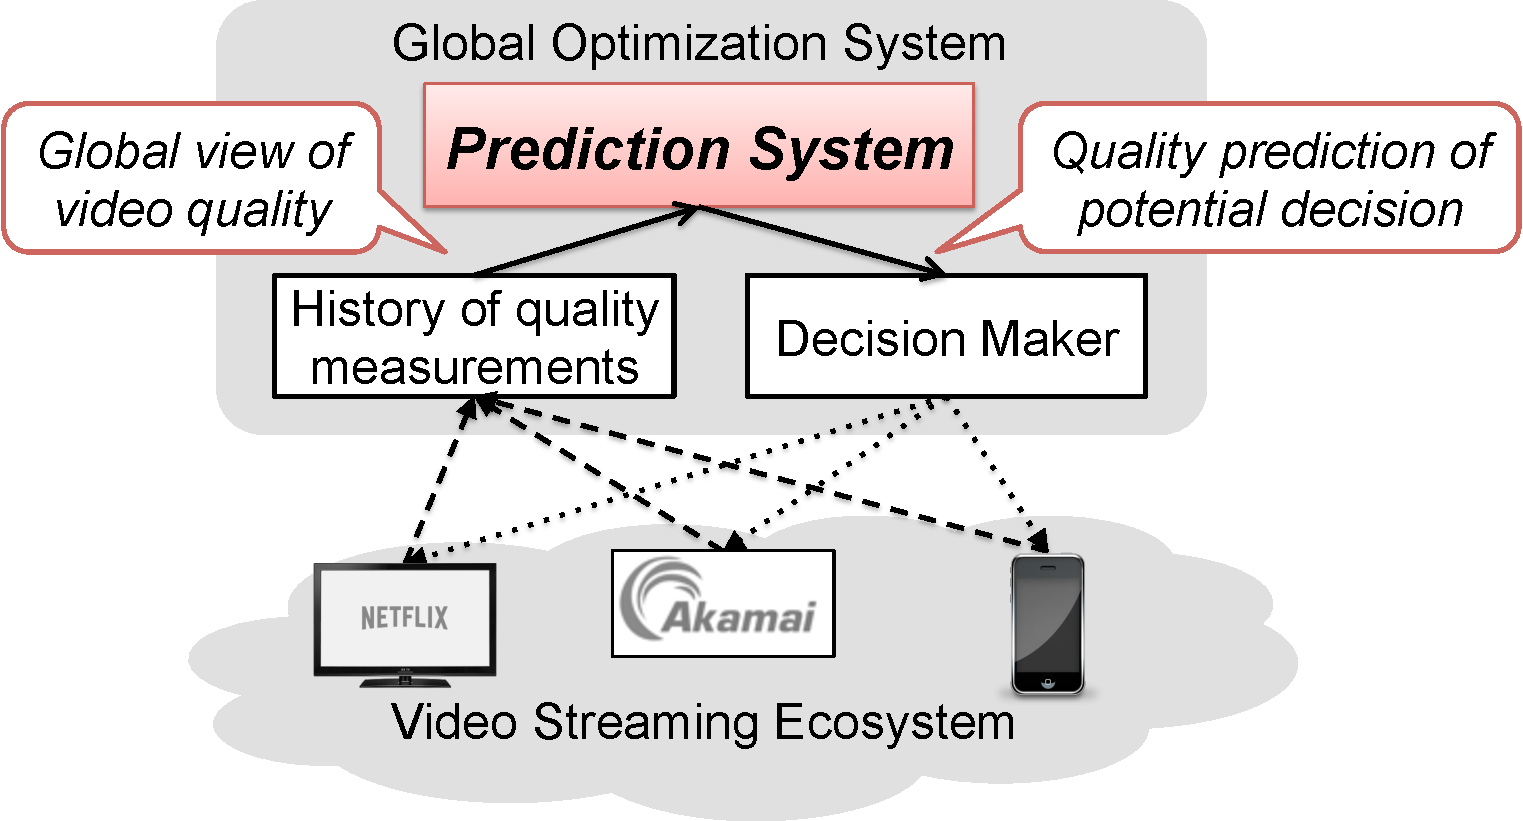
\includegraphics[width=.6\textwidth]{figures/cfa-controlplane-overview.pdf}
\caption{Overview of a \ControlPlane and the crucial role 
of a prediction system.}
\label{fig:globalsystem}
\end{figure}

In the context of video streaming, 
most video service providers today allow a 
video client (player) to switch CDN and bitrate 
among a set of available choices~\cite{sigcomm12,
c3,sigcomm12cdnmulti}.
%Today's video delivery systems allow each video client 
%(player) to switch CDN and bitrate among a set of 
%available choices. 
%\camera{Multi-CDN and multi-bitrate is commonly used by streaming video sites.}
These switches have little overhead and can be
performed at the beginning of and during a video 
playback~\cite{dash}. 
%\myparatight{Need for quality prediction}
Our goal then is to choose the best CDN and 
bitrate for a client by {\em accurately predicting 
the video quality of each hypothetical choice of 
CDN and bitrate}. 
In theory, if we can accurately predict the 
quality of each potential decision, then we 
can identify  the optimal decision.


To this end, we envision a prediction system that 
uses a {\em global view} of quality measurements to 
make predictions for a specific video session. % (i.e., pair of client and decision).
It learns a {\em prediction function} for each 
quality metric
$Pred:2^\HSessionFullSet\times\HSessionFullSet\mapsto \HReal$,
which takes as input a given set of historical 
sessions $\HSessionSet \in 2^\HSessionFullSet$ 
whose quality  is already measured, and a new 
session $\HSession\in\HSessionFullSet$, and 
outputs a quality prediction $p\in\HReal$ for 
$\HSession$.


%\myparatight{Quality metrics and session features} 
Each quality measurement %is a video session viewing a video 
summarizes the quality of a video session
for some duration of time (in our case, one minute). 
It is associated with values of four 
{\em quality metrics} (as defined in 
Section~\ref{subsec:related:video-qoe}) and 
a set of {\em features}
(summarized in Table~\ref{tab:features}).  
By feature,  we refer to the type of attribute 
(e.g., \fCDN), rather than value of these attributes 
(e.g., $\fCDN=Akamai$)
In general, the set of features depends on the degree 
of instrumentation and
what information is visible to a specific provider. 
For instance, a CDN may know the location of servers, 
whereas a third-party optimizer~\cite{conviva} may 
only have information at the CDN granularity. 
Our focus is not to determine the best set of 
features that should be recorded for each session, 
but rather engineer a prediction system that can 
take  an arbitrary set of features as inputs and 
extract the relationships between these features
and video quality. In practice, the above set of 
features can already provide accurate predictions 
that help improve quality.
% , and our approach can naturally include more
% features as they become available. 


\begin{table}[t!]
%\begin{footnotesize}
\begin{tabular}{p{3.8cm}|p{12cm}}
%{\bf Metrics} & {\bf Description} \\ \hline
%BufRatio & Fraction of time a session spends in buffering 
%(smooth playback is interrupted by buffering). \\ \hline
%AvgBitrate & Time-weighted average of bitrates in a session. \\ \hline
%JoinTime & Delay for the video to start playing from the 
%time the user clicks ``play''. \\ \hline
%Video start failure (VSF) & Fraction of sessions that fail to
% start playing (e.g., unavailable content or overloaded 
% server)\tablefootnote{For one session, VSF is zero if it 
% starts successfully, one otherwise.}. \\ \hline
{\bf Features} & {\bf Description} \\ \hline 
 \fASN &  Autonomous System to which client IP belongs. \\ \hline 
 \fCity &  City where the client is located.  \\ \hline
 \fConnectionType &  Type of access network; e.g.,  
 mobile/fixed wireless, DSL, fiber-to-home. \\ \hline
 \fPlayer & e.g.,  Flash, iOS, Silverlight,  HTML5. \\ \hline 
 \fSite & Content provider of requested video contents.\\ \hline%\tablefootnote{We use the terms site and content provider interchangeably.}. \\ \hline
 \fLiveOrVoD & Binary indicator of live vs.\ VoD content.\\ \hline 
 \fContentName & Name of the requested video object.\\ \hline 
 \fCDN &  CDN a  session started with. \\ \hline
 \fBitrate &  Bitrate value the session started at.
\end{tabular}
%\end{footnotesize}
\vspace{-0.2cm}
\caption{Quality metrics and session features associated 
with each session. 
\fCDN and \fBitrate refer to initial CDN/bitrate values as 
we focus on initial selections.}
\label{tab:features}
%\vspace{-0.5cm}
\end{table}

Our dataset consists of 6.6 million quality 
measurements collected from 2 million clients 
using 3 large public CDNs distributed across 
168 countries and 152 ISPs.

Next, we show real examples of the complex factors 
that impact video quality, and the limitations of strawman
solutions in capturing these relationships.

\subsection{Challenge 1: Complex QoE-Determining Factors}
\label{subsec:expressive}

\mypara{
High-dimensional relationship between video quality
and session features} 
Video quality could be impacted by {\em combinations} 
of multiple components in the network. 
Such high-dimensional effects make 
it harder to learn the relationships between video 
quality  and features, in contrast to simpler settings 
where features affect quality independently 
(e.g., assumed by Naive Bayes).
%quality prediction challenging since the 
%relationship between video quality and 
%features is more complex than if the impact of 
%individual features on quality is independent 
%(which is assumed by algorithms like Naive Bayes).




%\noindent\underline{Example of high dimensionality:}
%Here is an illustrative real-world example of high 
%dimensionality. 
In a real-world incident,
video sessions of Comcast users in Baltimore who watched 
videos from Level3 CDN experienced high failure rate (VSF) 
due to congested edge servers, shown by the blue line in 
Figure~\ref{fig:timeseries-expressive-model}.
The figure also shows the VSF of sessions sharing the same
values on one or two features with the affected sessions; 
e.g., all Comcast sessions across different cities and CDNs. 
In the figure, the high VSF of the affected sessions cannot be 
clearly identified if we look at the sessions 
 that match on only one or two features.
%does not suffice to clearly 
%none of the individual features or 
%two-feature combinations can clearly 
%show the high VSF of the affected sessions.
Only when three features of \fCDN (``Level3''), 
\fASN (``Comcast'') and \fCity (``Baltimore'') 
are specified (i.e., blue line), can we detect the 
high VSF and predict the quality of 
affected sessions accurately. 

\begin{figure}[t!]
\centering
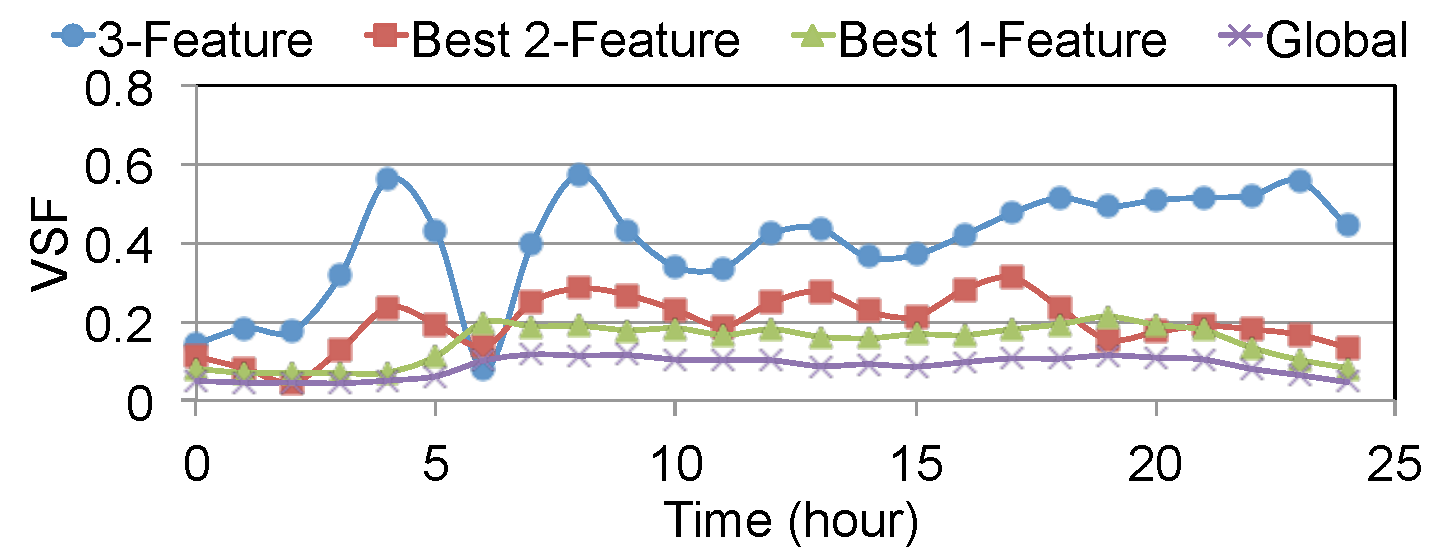
\includegraphics[width=0.65\textwidth]{figures/cfa-example-highdimension-timeseries.pdf}
\caption{The high VSF is only evident when three factors 
(CDN, ISP and geo-location) are combined.}
%\vspace{-0.2cm}
\label{fig:timeseries-expressive-model}
\end{figure}

 %One natural concern here is if this anecdotal evidence is an anomalous corner case.
% or if such high-dimensional 
%effects are  more pervasive. 
In practice, we find that such high-dimensional effects 
are the common case, rather than an anomalous corner case.  
For instance, more than 65\% of distinct
CDN-ISP-City values have VSF that is at least 50\% higher or 
lower than the VSF of sessions matching only one or 
two features (not shown). In other words, their quality is
affected by a combined effect of at least three features.

%\vyas{this doesnt address the concern. it  should have been across diff sessions/leaves :(}

\mypara{Limitation of existing solutions}
It might be tempting to develop  simple predictors; 
e.g., based on the last-hop 
connection by using average quality of history sessions 
with the same \fConnectionType value.
%\footnote{This is only an approximation to having the same last-hop capacity (we acknowledge that users of same connection type may have varying last-mile connection speed).}). 
However, they do not take into account the combined
impact of features on video quality.
Conventional machine learning techniques like Naive 
Bayes also suffer from the same limitation.
In Figures~\ref{subfig:quantitative-strawmen-lh} and 
\ref{subfig:quantitative-strawmen-nb},
we plot the actual JoinTime and the prediction
made by the last-hop predictor and Naive Bayes 
(from \texttt{Weka}~\cite{weka})
for 300 randomly sampled sessions.
The figures also show the mean relative error (
$\frac{|predicted-actual|}{actual}$).
For each session, the prediction algorithms train 
models using historical sessions within a 10-minute 
interval prior to the session under prediction.
It shows that the prediction error of both solutions is 
significant and two-sided (i.e., not fixable by
normalization).


\noindent{\bf Highly diverse structures of factors.}  
The factors that affect video quality vary across different sessions.
This means the prediction algorithm should be expressive enough
to predict quality for different sessions using 
different prediction models.
%\noindent\underline{Example of diversity:}
%Let us consider an illustrative example. 
%Many Flash video clients for whom Level3 
%edge servers provided high performance, and they had 
%good quality. 
%For these sessions, their quality is correlated with 
%a different set of features (\fCDN and \fPlayer) than 
%the example of high dimensionality (\fASN, \fCity and \fCDN).
For instance, the fact that many fiber-to-the-home (e.g., FiOS) 
users have high bitrates and people on 
 cellular connections have lower bitrates is largely due to 
the speed of their last-mile connection. In contrast, some video clients 
may experience video loading failures due to 
unavailability of specific content on some CDNs.
Chapter~\ref{ch:measurement}
has shown that many heterogeneous 
factors are correlated with video quality issues.
In Section~\ref{sec:cfa:outline}, we show  that 15\% of video 
sessions are impacted by more than 30 different combinations 
of features and give real examples of different factors that 
affect quality.

\noindent\underline{Limitation of existing solutions:}
To see why existing solutions are not sufficient, 
let us consider the $k$-nearest neighbor ($k$-NN) algorithm.
It does not handle diverse relationships between quality
and features, because the similarity between sessions
is based on the same function of features
independent of the specific session under prediction.
In Figure~\ref{subfig:quantitative-strawmen-nn},
we plot the actual values of JoinTime and the 
prediction made by $k$-NN with the same setup as 
Figure~\ref{subfig:quantitative-strawmen-lh}(b).
Similar to Naive Bayes and the last-hop predictor, 
$k$-NN has substantial prediction error.


\begin{figure}[t!]
\centering
\subfloat[Last hop (0.76)]
{
        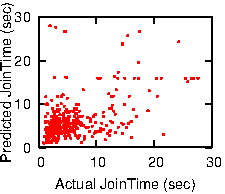
\includegraphics[width=0.3\textwidth]{figures/cfa-strawmen-scatter-comparison-naive.pdf}
        \label{subfig:quantitative-strawmen-lh}
}
\subfloat[Naive Bayes (0.61)]
{
        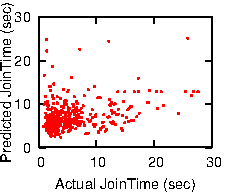
\includegraphics[width=0.3\textwidth]{figures/cfa-strawmen-scatter-comparison-2.pdf}
        \label{subfig:quantitative-strawmen-nb}
}
\subfloat[$k$-NN (0.63)]
{
        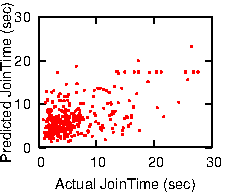
\includegraphics[width=0.3\textwidth]{figures/cfa-strawmen-scatter-comparison-1.pdf}
        \label{subfig:quantitative-strawmen-nn}
}
\caption{Prediction error of some existing solutions 
is substantial (mean of relative error in parentheses).}
%\vspace{-0.5cm}
\label{fig:quantitative-strawmen}
\end{figure}



\subsection{Challenge 2: Fresh Updates}
\label{subsec:fresh}

Video quality has significant temporal variability.
In Figure~\ref{fig:variability-all-metrics},
for each quality metric and combination of specific 
CDN, city and ASN, %(which reduces impact of the spatial variance), 
we compute the mean quality of sessions in each 
10-minute interval, and then plot the CDF of the 
relative standard deviation ($\frac{stddev}{mean}$)
%\footnote{Standard deviation divided by mean, which is used to normalize the scales of different quality metrics.} 
of the quality across different intervals.
In all four quality metrics of interest, we see 
significant temporal variability;
%on timescales of 10 minutes;
e.g., for 60\% of CDN-city-ASN combinations, 
the relative standard deviation of JoinTime across 
different 10-minute intervals is more than 30\%.
Such quality variability has also been confirmed in 
other studies (e.g.,~\cite{sigcomm12}).

The implication of such temporal variability
is that the prediction system must update models 
in near real-time.
In Figure~\ref{fig:strawman-staleness-all-metrics}, 
we use the same setup as 
Figure~\ref{fig:quantitative-strawmen}, except that the 
time window used to train prediction models is 
several minutes prior to the session under prediction.
The figure shows the impact of such staleness on 
the prediction error for JoinTime. 
For both algorithms, prediction error increases 
dramatically if the staleness exceeds 10 minutes. 
As we will see later, this negative impact of staleness 
on accuracy is not specific to these prediction 
algorithms (Section\ref{subsec:eval-scalability}). 
%This means the prediction system must update models  
%in near real-time.



\mypara{Limitation of existing solutions}
The requirement to use the most recent measurements
makes it infeasible to use computationally expensive models.
%models, such Support Vector Machines (SVM).
For instance, it takes at least one 
hour to train an SVM-based prediction model from 15K
quality measurements in a 10-minute interval for 
one video site, so the quality predictions 
will be based on information from more than one hour ago.


\begin{figure}[t!]
\centering
\subfloat[Temporal variability]
{
\includegraphics[width=.45\textwidth]{figures/cfa-stddev-metrics.pdf}
        \label{fig:variability-all-metrics}
}
\subfloat[Impact of staleness on accuracy]
{
\includegraphics[width=.45\textwidth]{figures/cfa-strawman-staleness.pdf}
        \label{fig:strawman-staleness-all-metrics}
}
\caption{Due to significant temporal variability of video quality (left), 
prediction error increases dramatically with stale data (right).}
%\vspace{-0.2cm}
\label{fig:temporal-variability}
\end{figure}


%In summary, the ideal predictor should (a) capture the 
%complex relationship between features and video 
%quality, and (b) predict quality based on fresh data. 

%We will present \dda to achieve these goals in the
%next sections.

%{
%\begin{table}[h!]
%%\begin{small}
%\begin{tabular}{p{6cm}|p{3.5cm}|p{3cm}}
%   &\textbf{Expressive models} & \textbf{Fresh updates} \\ \hline
%Naive models (e.g., last-mile)                       & $\times$          & $\checkmark$         \\ \hline
%Simple ML (e.g., NB, k-NN)                       & $\times$          & $\checkmark$         \\ \hline
%Complex ML (e.g., SVM)	                            & ?                 & $\times$             \\ \hline 
%{\bf The ideal (CFA)}                                 & {\bf $\checkmark$} & {\bf $\checkmark$}
%\end{tabular}
%%\end{small}
%%\vspace{-0.3cm}
%\caption{Analysis of existing solutions in the lense of the two challenges.}
%%\vspace{-0.2cm}
%\label{tab:qualitative-strawmen}
%\end{table}
%}














\section{Overview of CFA Ideas}
\label{sec:cfa:outline}


This section presents the domain-specific insights we use to 
help address the expressiveness challenge 
(Section~\ref{subsec:expressive}).  
The first insight is that sessions matching on all features 
have similar video quality.  
However, this approach suffers from the curse of dimensionality.
%it is challenging to translate this insight into an actionable approach because
%it suffers from the classical curse of dimensionality -- hard to find
%a sufficient number of identical sessions.  
Fortunately,  we can leverage a second insight that 
each video session has a subset of {\em critical features} 
that ultimately determine its video quality. 
 % and we can use  it to tackle the curse of dimensionality. 
We conclude this section  by highlighting two outstanding 
issues in translating these insights into  a practical 
prediction system.



\subsection{Baseline Prediction Algorithm}
\label{subsec:cfa:outline:basic}

Our  first insight is that 
%there is some inherent
%network/application structure because of which 
sessions that have identical  feature values will 
naturally have similar (if not identical) quality. 
 For instance, we expect that all Verizon 
 FiOS users  viewing a specific  HBO  video 
using Level3 CDN in Pittsburgh at Fri 9 am should 
have similar quality (modulo very user-specific  effects 
such as local Wi-Fi interference inside the home).
We can summarize the intuition as follows:

\begin{insight}
\vspace{0.1cm}
At a given time, video sessions having same value 
on every feature have similar video quality.
\vspace{-0.2cm}
\label{insight:1}
\end{insight}


%\camera{\insightref{insight:1} is merely a motivation.}
Inspired by \insightref{insight:1}, we can consider a 
baseline algorithm (Algorithm~\ref{alg:baseline}).
We predict a session's quality based on ``identical
sessions'', i.e., those from recent history that match 
values on {\em all} features with the session under 
prediction. 
Ideally, given infinite data, this 
%simple domain-specific engineered 
algorithm is accurate, because it can capture
all possible combinations of factors affecting 
video quality.


\begin{algorithm}[t!]
\begin{small}
 \KwIn{Session under prediction \HSession, Previous sessions \HSessionSet}
 \KwOut{Predicted quality $p$}
 \tcc{\footnotesize{$S'$:identical sessions matching on all features with \HSession in recent history(\HTimeWindowEst)}}
 $S'\leftarrow\HSimilarSessionSet{\HSession}{\HSessionSet}{AllFeatures}{\HTimeWindowEst}$\;
 \tcc{\footnotesize{Summarize the quality (e.g.,median) of the identical sessions in $S'$.}}
 $p\leftarrow\HEst{S'}$\;
 \Return{$p$}\;
\end{small}
 \caption{{\bf {\em Baseline prediction that finds sessions matching on all features and uses their 
 observed quality as the basis for prediction.  %Unfortunately, it suffers from the curse of dimensionality.
 }}}
\label{alg:baseline}
\end{algorithm}

 

%\begin{figure}[h!]
%\centering
%\includegraphics[width=0.4\textwidth]{eval-figs/batch-3/neighbor-count.pdf}
%\vspace{-0.1cm}
%\tightcaption{More than 90\% of sessions have at most one identical session within 5-min window.}
%\vspace{-0.1cm}
%\label{fig:infeasible-nn}
%\end{figure}

However, this algorithm is unreliable as it suffers from the 
classical curse of 
dimensionality~\cite{powell2007approximate}. 
Specifically, given the number of combinations 
of feature values (ASN, device, content providers, 
CDN, just to name a few), it is hard to find enough identical 
sessions needed to make a robust prediction. 
In our dataset, more than 78\% of sessions have no 
identical session (i.e., matching on all features)
within the last 5 minutes.
%more than 78\% of sessions within a 5-minute time window
%have no identical session (i.e., matching on all features).
%Thus, we do not have sufficient data to make reliable predictions.


\subsection{Critical Features}
\label{subsec:cfa:outline:critical}

 In practice, we expect that some features are
more likely to  ``explain'' the observed quality 
of a specific video session than others.  
For instance, if a specific peering point
between Comcast and Netflix in New York is 
congested, then we expect most of these users 
will suffer poor quality, regardless of the speed of 
their local connection. 
%Similarly, we can roughly expect most 
% fiber-to-the-home (e.g., FiOS) users to have high bitrates and people on 
% cellular connections to have lower bitrates. We can formalize this as follows:

\begin{insight}
\vspace{0.1cm}
Each video session has a subset of {\em critical features} that ultimately determines its video quality.
\vspace{-0.2cm}
\end{insight}

We already saw some real examples in 
Section~\ref{subsec:expressive}:
%To see some real-world examples of critical features, we 
%consider two examples in \Section\ref{subsec:expressive}.
in the example of high dimensionality, the critical features 
of the sessions affected by the congested Level3 edge 
servers are $\{\fASN, \fCDN, \fCity\}$;
in the examples of diversity, the critical features are
$\{\fConnectionType\}$ and $\{\fCDN,\fContentName\}$.
Table~\ref{tab:bottleneck} gives more real examples 
of critical features that we have observed in operational 
settings and confirmed with domain experts.


\begin{table}[t!]
%\begin{small}
    \begin{tabular}{p{2.in}|p{2in}}
    {\bf Quality issue} & {\bf Set of critical features} \\ \hline\hline
%    Software update on OS & \{OS\}  \\ \hline
%    Player bitrate-adaptation logic & \{PlayerName\}  \\ \hline
%    Device  on cellular signal  & \{Device,ConnectionType\}  \\ \hline
%    Load of CDN1 server in city  & \{CDN,City\}      \\ \hline
%    Link congestion between CDN1 server in city and ASN    & \{CDN,City,ASN\}    \\ \hline
%    Bad Live feeds from one site to CDN1  & \{Site,LiveOrVod,CDN\} \\

     Issue on one player of Vevo & $\{\fPlayer,\fSite\}$ \\ \hline
     ESPN flipping between CDNs  & $\{\fCDN,\fSite,\fContentName\}$ \\ \hline
     Bad Level3 servers for Comcast users in Maryland& $\{\fCDN,\fCity,\fASN\}$ \\
    \end{tabular}
\caption{Real-world examples of critical features confirmed 
by analysts at a large video optimization vendor.}
\label{tab:bottleneck}
%\end{small}
%\vspace{-0.2cm}
\end{table}


A natural implication of this insight is that it can help us 
tackle  the curse of dimensionality.
Unlike Algorithm~\ref{alg:baseline}, which fails to find a 
sufficient number of sessions,
%Instead of failing to find a sufficient number of identical sessions that match on all 
%features (Algorithm~\ref{alg:baseline}), 
we can estimate quality more reliably by aggregating 
observations across a larger amount of ``similar sessions'' that 
only need to match on these {\em critical features}. 
Thus, critical features can provide expressiveness
while avoiding curse of dimensionality.

Algorithm~\ref{alg:critical-feature} presents a logical 
view of this idea:
%We use two logical steps to predict quality of session  $\HSession$.
\begin{packedenumerate}
\item {\bf Critical feature learning (line 1):} 
First, find the critical features of each session $\HSession$, 
denoted as $\HCriticalFeature{\HSession}$.
\item {\bf Quality estimation (line 2, 3):}
Then, find similar sessions that match values with 
$\HSession$ on critical features 
$\HCriticalFeature{\HSession}$ 
within a recent history of length $\HTimeWindowEst$ 
(by default, 5 minutes). 
Finally, return some suitable estimate of the quality of 
these similar sessions; 
e.g., the median\footnote{We use median because it 
is more robust to outliers.} 
(for BufRatio, AvgBitrate, JoinTime) or the mean (for VSF).
\end{packedenumerate}



\begin{algorithm}[t!]
\begin{small}
 \KwIn{Session under prediction \HSession, Previous sessions \HSessionSet}
 \KwOut{Predicted quality $p$}
 \tcc{\footnotesize{$CF_{\HSession}$:Set of critical features of \HSession}}
 $CF_{\HSession}\leftarrow\HCriticalFeature{\HSession}$\;
 \tcc{\footnotesize{$S'$:Similar sessions matching values on 
critical features $CF_{\HSession}$ with \HSession.}}
 $S'\leftarrow\HSimilarSessionSet{\HSession}{\HSessionSet}{CF_{\HSession}}{\HTimeWindowEst}$\;
 \tcc{\footnotesize{Summarize the quality of the similar sessions in $S'$.}}
 $p\leftarrow\HEst{S'}$\;
 \Return{$p$}\;
\end{small}
 \caption{{\bf {\em \dda prediction algorithm, where prediction is based on 
similar sessions matching on critical features.}}}
\label{alg:critical-feature}
\end{algorithm}



A practical benefit of Algorithm~\ref{alg:critical-feature} 
is that it is interpretable~\cite{vellido2012making}, 
unlike some machine learning algorithms (e.g., PCA or SVM).
%quality predictions are interpretable.
This allows domain experts to combine their knowledge 
with \dda
%(e.g., directly setting critical features of sessions) 
and diagnose prediction errors or resolve incidents, 
as we explore in Section~\ref{subsec:insight-value}. 

At this time, it is useful to clarify what critical features 
are and what they are not.
In essence, critical features provide the explanatory 
power of how a prediction is made.
However, critical features are not a minimal set of 
factors that determine the quality (i.e., root cause). 
That is, they can include both features that reflect 
the root cause as well as additional features.
For example, if all HBO sessions use Level3, their 
critical features may include both \fCDN and \fSite, 
even if \fCDN is redundant, since including it does 
not alter predictions. 
The primary objective of \dda is accurate prediction; 
root cause diagnosis may be an added benefit.







\section{Design of CFA}
\label{sec:cfa:design}

In this section, we present the detailed design of \dda 
and discuss how we address the two practical challenges 
mentioned in the previous section: learning critical features 
and reducing update delay.

The key  to addressing these challenges
%,  which leads 
% to the practical realization of \dda, 
 is our third and final domain-specific insight:

\begin{insight}
\vspace{0.1cm}
Critical features tend to {\em persist} on long timescales
of tens of minutes.
\vspace{-0.2cm}
\label{insight:persistence}
\end{insight}

 This insight is derived from prior measurement 
 studies.
 For instance, our measurement study in 
 Chapter~\ref{ch:measurement} 
 on shedding light on video quality issues in the wild showed 
 that the factors that lead to poor video quality persist
 for hours, and sometimes even days.  
 Another recent study from the C3 system suggests that 
 the best CDN tends to be relatively stable on the 
 timescales of few tens of minutes~\cite{c3}.  
We independently confirm this observation in 
Section~\ref{subsec:eval-scalability} that 
using slightly stale critical features (e.g., 30-60 minutes 
 ago) achieves similar prediction accuracy as using the 
most up-to-date critical features.
Though this insight holds for most cases, it is still possible
(e.g., on mobile devices) that critical features persist on a 
relatively shorter timescale (e.g., due to the nature of 
mobility).
%For instance, on a mobile device, the persistency of critical features
%might be shorter than tens of minutes due to the nature of mobility.}


% we show that using slightly stale 
%^critical features (i.e., learned 30-60 minutes ago) achieves
%s%imilar prediction accuracy as using the most up-to-date 
%c%ritical features, suggesting that the persistence of critical 
%features is on timescale of tens of minutes.

Note that the persistence of critical features does not 
mean that quality values are equally persistent.  
In fact, persistence of critical features is on a 
timescale an order of magnitude longer than 
the persistence of quality.  
That is, even if quality fluctuates rapidly, the critical 
features that determine the quality do not change 
as often.


As we will see below, this persistence enables 
(a) automatic learning  of critical features from history, 
and (b) a scalable workflow that provides 
up-to-date estimates. 


\subsection{Learning Critical Features}
\label{subsec:cfa:design:learning}

Recall that the first challenge is
% that we cannot statically map each
%session to its critical features 
obtaining the critical features for each session.
The  persistence of  critical features has a natural 
corollary that we can use to automatically learn them: 

\begin{imp}
\vspace{0.1cm}
Persistence  implies that 
critical features of a session are learnable from history.
\vspace{-0.6cm}
\label{imp:learning}
\end{imp}

%The key notation is {\em \HSimSessSet}
%$\HSimilarSessionSet{\HSession}{\HSessionSet}{\HFeatureSet}{\HTimeWindow}$, which consists of sessions in $\HSessionSet$ that match $\HSession$ on features in $\HFeatureSet$ and happened within time window $\HTimeWindow$ before $\HSession$. 
%For instance, $\HSimilarSessionSet{\HSession}{\HSessionSet}{\{CDN\}}{\textrm{5 minutes}}$ 
%includes all sessions that use same CDN with $\HSession$ 
%and happened within 5 minutes before $\HSession$. 
%Note that, prediction made by Algorithm~\ref{alg:critical-feature} is 
%$\HPred{\HSession}{\HSessionSet}=\HEst{\HSimilarSessionSet{\HSession}{\HCriticalFeature{\HSession}}{\HFeatureSet}{\HTimeWindow}}$.


\begin{table}[t!]
%\begin{footnotesize}
\begin{tabular}{p{3.5cm}|p{3cm}|p{7.5cm}}
{\bf Notations} & {\bf Domains} & {\bf Definition} \\ \hline\hline
$\HSession,\HSessionSet,\HSessionFullSet$ & & A session, a set of sessions, set of all sessions \\ \hline
%$\HSession$ & & A video session \\ \hline
%$\HSessionSet$ & & A set of video sessions \\ \hline
%$\HSessionFullSet$ & & Set of all video sessions \\ \hline
%$\HSessionTime{\HSession}$ & $\HSessionFullSet\mapsto\HReal$ & Timestamp of $\HSession$ \\ \hline
$\HSessionQuality{\HSession}$ & $\HSessionFullSet\mapsto\HReal$ & Quality of $\HSession$ \\ \hline
$\HDistribution{\HSessionSet}$ & $2^\HSessionFullSet\mapsto2^\HReal$ & $\{\HSessionQuality{\HSession}|\HSession\in\HSessionSet\}$ \\ \hline
%$\HEst{\HSessionSet}$ & $2^\HSessionFullSet\mapsto\HReal$ & Summarizing value (by default, median) of $\HDistribution{\HSessionSet}$ \\ \hline
%$\HDist{\HSessionSet_1}{\HSessionSet_2}$ & $2^\HSessionFullSet\times2^\HSessionFullSet\times\HReal$ & JS divergence of $\HDistribution{\HSessionSet_1}$ and $\HDistribution{\HSessionSet_2}$\\ \hline
$\HFeature,\HFeatureSet,\HFeatureFullSet$ & & A feature, a set of features, set of all features \\ \hline
%$\HFeature$ & & A session feature \\ \hline
%$\HFeatureSet$ & & A set of session features \\ \hline
%$\HFeatureFullSet$ & & Set of all session features \\ \hline
$\HCriticalFeature{\HSession}$ & $\HSessionFullSet\mapsto2^\HFeatureFullSet$ & Critical features of $\HSession$ \\ \hline
$\HFeatureValueFullSet$ & & Set of all feature values \\ \hline
$\HFeatureValue{\HFeature}{\HSession}$ & $\HFeatureFullSet\times\HSessionFullSet\mapsto\HFeatureValueFullSet$ & Value on feature $\HFeature$ of $\HSession$ \\ \hline
$\HFeatureSetValue{\HFeatureSet}{\HSession}$ & $2^\HFeatureFullSet\times\HSessionFullSet\mapsto2^\HFeatureValueFullSet$ & Set of values on features in $\HFeatureSet$ of $\HSession$ \\ \hline
$SimilarSessionSet$ $(\HSession,\HSessionSet,\HFeatureSet,\HTimeWindow)$ & $\HFeatureFullSet\times2^\HFeatureFullSet\times\HSessionFullSet\times\HReal^{+}\mapsto2^\HFeatureFullSet$ & $\{\HSession'|\HSession'\in\HSessionSet,\HSessionTime{\HSession}-\HTimeWindow<\HSessionTime{\HSession'}<\HSessionTime{\HSession},\HFeatureSetValue{\HFeatureSet}{\HSession'}=\HFeatureSetValue{\HFeatureSet}{\HSession}\}$ \\ 
%\hline
%$\HPred{\HSession}{\HSessionSet}$ & $\HSessionFullSet\times2^\HSessionFullSet\mapsto\HReal$ & Prediction function
\end{tabular}
%\end{footnotesize}
\caption{Notations used in learning of critical features.}
\label{tab:terminology}
%\vspace{-0.5cm}
\end{table}



Specifically, we can simply look back over the history and identify  
the subset of features $\HFeatureSet$ such that the quality 
distribution of sessions matching on $\HFeatureSet$ is most similar 
to that of sessions matching on {\em all} features.   
For instance, suppose we have three features
$\langle \mathit{ContentName},\mathit{ASN},\mathit{CDN}\rangle$ and 
it turns out that sessions with  $\mathit{ASN}=\mathit{Comcast},
\mathit{CDN}=\mathit{Level3}$ consistently
have  high buffering over the last few hours due to some internal 
congestion at the corresponding exchange point. 
Then, if we look back over the last few hours, the data from 
history will   naturally reveal  that the distribution of the quality of 
sessions  with the feature values
$\langle\mathit{ContentName}=\mathit{Foo},
\mathit{ASN}=\mathit{Comcast},\mathit{CDN}=\mathit{Level3}\rangle$
will be  similar to $\langle \mathit{ContentName}=\mathit{*},
\mathit{ASN}=\mathit{Comcast},\mathit{CDN}=\mathit{Level3} \rangle$, 
but very different from, say, the quality of sessions in 
$\langle \mathit{ContentName}=\mathit{*},\mathit{ASN}=\mathit{*},
\mathit{CDN}=\mathit{Level3} \rangle$,
or $\langle \mathit{ContentName}=\mathit{*},
\mathit{ASN}=\mathit{Comcast},\mathit{CDN}=\mathit{*} \rangle$.
Thus, we can use a data-driven approach to learn that 
$\mathit{ASN},\mathit{CDN}$ are the critical features for sessions 
matching $\langle \mathit{ContentName}=\mathit{Foo},
\mathit{ASN}=\mathit{Comcast},\mathit{CDN}=\mathit{Level3} \rangle$.




% irrespective  of other feature values, sessions wit history that predicting the quality 
  



%Inspired by \impref{imp:learning}, we learn critical features 
%over a time window, during which critical features persist. 
%Intuitively, critical features are the subset of features 
%that meet two requirements.
%\begin{packeditemize}
%\item First, there should enough sessions
%for quality estimation of Algorithm~\ref{alg:critical-feature}
%to avoid unreliable prediction due to curse of dimensionlity.
%This is guaranteed by line 7-9.
%\item Second, among subsets of features that meet the first 
%requirement, we find the subset of features $\HFeatureSet$ such that 
%quality distribution of sessions matching $\HFeatureSet$ is the 
%most similar to that of sessions matching all features
%, 
%because these two sets of sessions should be determined by 
%the same set of critical features.
%\end{packeditemize}
%Finally, we should take into account two key aspects of model 
%expressiveness (\Section\ref{subsec:expressive}):
%high diversity (critical features are learned for each session 
%under prediction), and high dimensionality (critical features could be 
%any subsets of features). 


\begin{algorithm}[t!]
\begin{small}
 \KwIn{Session under prediction \HSession, Previous sessions \HSessionSet}
 \KwOut{Critical features for  \HSession}
 \tcc{Initialization}
 $\mathit{MaxSimilarity}\leftarrow-\infty,\mathit{CriticalFeatures}\leftarrow \mathit{NULL}$\;
 %\tcc{$D_{finest}$:Quality distribution of \HSimilarSessionSet{\HSession}{\HSessionSet}{\HFeatureFullSet}{\HTimeWindowLearn}.}
 \tcc{$D_{finest}$:Quality distribution of sessions matching on $\HFeatureFullSet$ in $\HTimeWindowLearn$.}
 $D_{finest}\leftarrow\HDistribution{\HSimilarSessionSet{\HSession}{\HSessionSet}{\HFeatureFullSet}{\HTimeWindowLearn}}$\;
 \For{$\HFeatureSet\subseteq2^\HFeatureFullSet$}{
	\tcc{Exclude $\HFeatureSet$ without enough similar sessions for prediction.}
	\If{$|\HSimilarSessionSet{\HSession}{\HSessionSet}{\HFeatureSet}{\HTimeWindowEst}|<n$}{{\bf continue\;}}
 	%\tcc{$D_{\HFeatureSet}$:Quality distribution of \HSimilarSessionSet{\HSession}{\HSessionSet}{\HFeatureSet}{\HTimeWindowLearn}.}
	\tcc{$D_{\HFeatureSet}$:Quality distribution of sessions matching on $\HFeatureSet$ in $\HTimeWindowLearn$.}
	$D_{\HFeatureSet}\leftarrow\HDistribution{\HSimilarSessionSet{\HSession}{\HSessionSet}{\HFeatureSet}{\HTimeWindowLearn}}$\;
	\tcc{Get similarity of $D_{finest}$ \& $D_{\HFeatureSet}$.}
	$\mathit{Similarity}\leftarrow\HDist{D_{\HFeatureSet}}{D_{finest}}$\; 	\If{$\mathit{Similarity}>\mathit{MaxSimilarity}$}{
		$\mathit{MaxSimilarity}\leftarrow \mathit{Similarity}$\;
		$\mathit{CriticalFeatures}\leftarrow \HFeatureSet$\;
	}
 }
 \Return{CriticalFeature}\;
\end{small}
 \caption{{\bf {\em Learning of critical features.}}}
\label{alg:learning}
\end{algorithm}

Algorithm~\ref{alg:learning}  formalizes this intuition for learning 
critical features. 
Table~\ref{tab:terminology} summarizes the notation used in
Algorithm~\ref{alg:learning}.
For each subset of features $\HFeatureSet$ (line 3), 
we compute the similarity between the quality distribution 
($D_{\HFeatureSet}$) of sessions matching on $\HFeatureSet$ 
and the quality distribution ($D_{finest}$) of sessions
matching on all features (line 7). 
% \vyas{please refer to the pseudocode in the text with the line numbers etc. dont just 
%assume ppl will read pseudocode and follow!!}
Then, we find the $\HFeatureSet$ that yields the maximum 
similarity (line 8-10), under one additional constraint that 
$\HSimilarSessionSet{\HSession}{\HSessionSet}{\HFeatureSet}{\HTimeWindowEst}$ 
should include enough (by default, at least 10) sessions to get 
reliable quality estimation (line 4-5).
%there
%should be enough sessions to  get reliable quality
%estimates, i.e., $\HSimilarSessionSet{\HSession}{\HSessionSet}{\HFeatureSet}{\HTimeWindowEst}$
%needs to have at least $n$ (by default, 10) sessions (line 4-5).
This check ensures that the algorithm will not simply return the set of all features.



As an approximation of the duration in which critical features 
persist, we use $\HTimeWindowLearn=60min$.
Note that $\HTimeWindowLearn$ is an order of magnitude 
larger than the time window $\HTimeWindowEst$ used in 
quality estimation, because critical features persist on a 
much longer timescale than quality values.
%Default value of $n$ is 10 sessions. 
We use (the negative of) Jensen-Shannon 
divergence between $D_1$ and $D_2$ to quantify their 
similarity $\HDist{D_1}{D_2}$.
%(assuming both of them are draw from a normal distribution).





Although Algorithm~\ref{alg:learning} can handle most cases, 
there are corner cases where
$\HSimilarSessionSet{\HSession}{\HSessionSet}
{\HFeatureFullSet}{\HTimeWindowLearn}$ 
does not have enough sessions (i.e., more than $n$) to 
%learn $\HCriticalFeature{\HSession}$ reliably. 
compute $\HDist{D_{\HFeatureSet}}{D_{finest}}$ reliably. 
In these cases, we replace $D_{finest}$ by the set of $n$ 
sessions that share most features with $\HSession$ 
over the time window of $\HTimeWindowLearn$. 
Formally, we use 
$\{\HSession'|\HSession'\textrm{ matches $k_{\HSession}$ 
features with }\HSession\}$, 
where $k_{\HSession}=\argmin_k\left(|\{\HSession'|\HSession'\textrm{ matches $k$ features with }\HSession\right|\geq n\}|)$.





\subsection{Using Fresh Updates}
\label{subsec:scalability}

Next, we focus on reducing the update delay
between when a quality measurement is received and 
used for prediction. 



Naively running critical feature learning and quality 
estimation of Algorithm~\ref{alg:critical-feature}
can be time-consuming, causing the predictions to 
rely on stale data.
In Figure~\ref{fig:scalable-workflow}(a), $T_{CFL}$ and 
$T_{QE}$ are the duration of critical feature learning and 
the duration of quality estimation, respectively. 
The staleness of quality estimation (depicted in 
Figure~\ref{fig:scalable-workflow}) 
to respond to a prediction query can be as large as the 
total time of two steps (i.e., $T_{CFL}+T_{QE}$), which 
typically is tens of minutes 
(Section~\ref{subsec:eval-scalability}).
%This is because the critical feature learning (line 1) typically takes tens of 
%minutes to update its results (\Section\ref{subsec:eval-scalability}).
%To see why, consider Figure~\ref{fig:scalable-workflow}(a), where $T_{CFL}$ and $T_{QE}$ are the duration
%of critical feature learning and the duration of quality estimation, respectively. 
%To respond a prediction query, the staleness of quality estimation is up to the total time 
%of two steps (i.e., $T_{CFL}+T_{QE}$).
Also, simply using more parallel resources is not sufficient. 
The time to learn critical features using
Algorithm~\ref{alg:learning} grows linearly with the number of 
sessions under prediction, the number of history sessions,
and the number of possible feature combinations.
Thus, the complexity of learning critical features $T_{CFL}$ is 
exponential in the number of features. Given the current 
set of features, $T_{CFL}$ is on the scale of tens of minutes.

%This means the complexity of learning critical features is 
%super-linear to the size of data (number of sessions and 
%number of available features). Thus, simply adding more 
%resources will not suffice.

\begin{figure}[t!]
\centering
%\vspace{-0.3cm}
%\hspace{-0.6cm}
%\subfigure[Naive workflow]
%{
%\includegraphics[width=0.25\textwidth]{figures/scalability-naive.pdf}
%\label{subfig:scalability-naive}
%}
%\hspace{-0.4cm}
%\subfigure[CFA workflow]
%{
%\includegraphics[width=0.25\textwidth]{figures/scalability-cfa.pdf}
%\label{subfig:scalability-cfa}
%}
%\hspace{-0.6cm}
\includegraphics[width=0.85\textwidth]{figures/cfa-scalability-naive-cfa.pdf}
\caption{To reduce update delay, we run critical feature learning 
and quality estimation at different timescales by leveraging 
persistence of critical features.}
\label{fig:scalable-workflow}
\end{figure}

To reduce update delay, we again leverage the 
persistence of critical features:

\begin{imp}
\vspace{0.1cm}
Persistence implies that critical features can be cached and reused
 over tens of minutes.
 \vspace{-0.3cm}
\label{imp:reducing}
\end{imp}


 Building on \impref{imp:reducing}, we decouple the 
critical feature learning and quality estimation steps, and run
them at separate timescales.
On the timescale of tens of minutes, we update the results of 
critical feature learning. Then, on a faster timescale of tens of seconds, 
we update quality estimation using fresh data and the most recently
learned critical features. 

This decoupling 
%ensures that each step 
%can update its result sufficiently frequently to 
minimizes the impact of staleness on prediction accuracy.
Learning critical features on the timescale of tens 
of minutes
%\camera{\footnote{Learning critical features on a much larger set of features could take longer, 
%but it is enough for the current set of features, and the feature set will not grow very quickly.}}
is sufficiently fast as they persist 
on the same timescale.
%Since critical features persist, learning them
%on the timescale of tens of minutes is sufficient to capture their dynamics.
Meanwhile, %based on learned critical features, 
quality estimation can be updated every tens of seconds 
and makes predictions based on quality updates with sufficiently
low staleness.
Thus, the staleness of quality estimation $T_{QE}$ of
the decoupled workflow (Figure~\ref{fig:scalable-workflow}(b))
is a magnitude lower than $T_{QE}+T_{CFL}$ of the naive workflow 
(Figure~\ref{fig:scalable-workflow}(a)).
In Section~\ref{subsec:eval-scalability}, we show that 
this workflow can retain the freshness of critical features and quality estimates.
%\camera{It should be noticed that, though $T_{QE}+T_{CFL}$ (tens of minutes) 
%is not long enough to handle any number of features, 
%it is enough for \dda to learn critical features from the current feature set, 
%and the feature set will not grow very quickly.}


In addition, \dda has a natural property that two sessions sharing 
all feature values and occurring close in time will map to the 
same critical features. Thus, instead of running the steps 
per-session, we can reduce the computation to the granularity of 
{\em \leafs}, i.e., distinct values of all features.


\subsection{Putting It Together}

Building on these insights, we create 
the following practical {\em three-stage} workflow of \dda.

\begin{packeditemize}

\item {\bf Stage I: Critical feature learning} 
(line 1 of Algorithm~\ref{alg:critical-feature}) runs offline, say, 
every tens of minutes to an hour.  The output of this stage is a 
key-value table called {\em critical feature function} that maps 
all observed \leaf{s} to their critical features.

\item {\bf Stage II: Quality estimation} 
(line 2,3 of Algorithm~\ref{alg:critical-feature}) runs every tens of seconds 
for all observed \leafs based on the most recent critical features 
learned in the first stage.  
This outputs another key-value table called {\em quality function}
that maps a \leaf to the quality estimation, by aggregating the most 
recent sessions with the corresponding critical features.


\item {\bf Stage III: Real-time query/response.} Finally, we 
provide real-time query/response on the arrival of each client,
operating  at the millisecond timescale, by simply looking up the 
most recent precomputed value function from the previous stage.  
These operations are simple and can be done very fast.

\end{packeditemize}
 
%There are two heuristic (optional) optimizations we implement. 
%In the interest of brevity, we discuss them briefly since the above workflow above is the main contributor to scalability. 
%First, we can focus on a small fraction of most popular \leafs and still cover a substantial fraction of sessions in the future. 
Finally, instead of forcing all \leaf-level computations to run in every 
batch, we can do triggered recomputations of critical feature learning 
only when the observed prediction errors are high.



\section{Implementation and Deployment}
\label{sec:cfa:impl}

This section presents our implementation of \dda 
 and highlights engineering solutions to address practical challenges 
 in operational settings (e.g., avoiding bulk data loading and 
speeding up development iterations).

\subsection{Implementation of \dda Workflow}
\label{subsec:cfa:impl:workflow}

%Recall that \dda logically consists of three stages 
%running at different timescales (\Section\ref{subsec:scalability}). 
\dda's three stages are implemented in two different locations:
a centralized backend cluster and geographically 
distributed frontend clusters as depicted in Figure~\ref{fig:impl}. 


\begin{figure}[t!]
\centering
\includegraphics[width=.55\textwidth]{figures/cfa-impl-overview.pdf}
\vspace{-0.1cm}
\caption{Implementation overview of \dda. The three stages of 
\dda workflow are implemented in a backend cluster and distribute
frontend clusters.}
%\vspace{-0.2cm}
\label{fig:impl}
\end{figure}

\mypara{Centralized backend} 
The critical feature learning and quality 
estimation stages are implemented in a backend 
cluster as periodic jobs. 
By default, critical feature learning runs every 30 
minutes, and quality estimation runs every minute. 
A centralized backend is a natural choice because 
we need  a global view of all quality measurements.
The quality function, once updated by the estimation 
step, is disseminated to distributed 
frontend clusters using Kafka~\cite{kreps2011kafka}.

%backend cluster is two-fold.
%First, the backend has the access to the database of 
%all quality measurements, which is needed by critical 
%feature learning and quality estimation.
%Second, they are not required to be as much responsive to client 
%requests as real-time query/response. 

%For real-time query/response to use the up-to-date 
%quality function (i.e., a map between a \leaf and 
%quality estimation), 

Note that we can further reduce learning time
 using simple parallelization strategies. 
%(As discussed in \Section\ref{subsec:scalability}, parallelization alone does not provide a scalable workflow).  
Specifically, the critical features of different \leafs 
can be learned independently.
Similarly in Algorithm~\ref{alg:learning}, the 
similarity  of quality distributions can be 
computed in parallel. 
To exploit this data-level parallelism, 
we implement them as Spark jobs~\cite{spark}. 



\mypara{Distributed frontend} 
%Real-time query/response to prediction queries 
%is implemented in distributed frontend clusters, 
%where decision makers  (which selects CDN, 
%bitrate for clients) are located~\cite{c3}.
Real-time query/response and 
decision makers of CDN/bitrate are co-located in 
distributed frontend clusters that are closer to 
clients than the backend.
%Pushing real-time query/response and 
%decision maker to distributed frontend 
Each frontend cluster receives the quality function 
from the backend and caches it locally for fast
prediction.
This reduces the latency of making decisions 
for clients.
 




%The learning of critical feature function and quality 
%functions on different ``\leafs'' is independent. 
%Critical feature learning can simultaneously 
%evaluate the distribution similarity in 
%Algorithm~\ref{alg:learning} of multiple feature 
%combinations in one ``Map'' operation and find the 
%critical feature in one ``Reduce'' operation. 
%To exploit such parallelism, these two stages are 
%implemented as Spark MapReduce jobs~\cite{spark}. 



\subsection{Challenges in an Operational Setting}
\label{subsec:cfa:impl:challenge}

%Next, we highlight some operational experience from the 
%deployment of \dda in a production system.

\mypara{Mitigating impact of bulk data loading} 
%Resources, such as bandwidth and cluster nodes 
%(sender/receivers) between the quality measurement 
%database and 
The backend cluster is shared 
and runs other delay-sensitive 
jobs; e.g.,  analytics queries from production teams. 
 Since the critical feature learning runs periodically 
and loads a large amount of data ($\approx$30 
GB), it creates spikes in the delays of other jobs 
(Figure~\ref{fig:completion-delay}).  
To address this concern, we engineered a simple 
heuristic to evenly spread the data retrieval where  
we load a small piece of data every few minutes. 
As Figure~\ref{fig:completion-delay} shows, this 
reduces the spikes caused by bulk data loading in 
batch mode.
Note that this does not affect critical feature learning.


\begin{figure}[t!]
\centering
\includegraphics[width=.8\textwidth]{figures/cfa-smooth-batch-timeseries.pdf}
%\vspace{-0.3cm}
\caption{Streaming data loading has smoother 
impact on completion delay than batch data loading.}
%\vspace{-0.4cm}
\label{fig:completion-delay}
\end{figure}

\mypara{Iterative algorithm refinement}
Some parameters (e.g., learning window size 
\HTimeWindowLearn) of \dda require iterative tuning in a 
production environment.
%However, one practical challenge arises  due to code release cycles.
However, one practical challenge is that the 
frontend-facing part of the backend can 
only  be updated once every couple of weeks 
due to code release cycles. 
Thus,  rolling out new prediction algorithms may 
take several days and is a practical concern.
Fortunately, the decoupling between critical feature 
learning and quality estimation 
(Section~\ref{subsec:scalability})
means that changes to critical feature learning
are confined to the backend cluster. 
This enables us to rapidly refine 
and customize the \dda algorithm. 
% (Without this decoupling, any changes to \dda 
%would also need to update quality estimation in the front-end facing part of
%the backend, and would be have slow refresh cycles.)



\section{Evaluation}
\label{sec:cfa:eval}


In this section, we show that:
\begin{packeditemize}
\item \dda  predicts video quality with 30\% less error than 
competing machine learning algorithms 
(Section~\ref{subsec:eval-accuracy}).
\item Using \dda-based prediction, we can improve  
video quality significantly; e.g., 32\% less BufRatio, 
12\% higher AvgBitrate in a pilot deployment 
(Section~\ref{subsec:eval-improvement}).
% than those selected by a baseline players. 
%More extensive trace-driven simulation shows that across different quality metrics, \dda leads to 5-17\% improvement over decisions made by the more accurate prediction algorithms other than \dda.
\item \dda is responsive to client  queries and  makes 
predictions based on the most recent critical features 
and quality measurements 
(Section~\ref{subsec:eval-scalability}).
\end{packeditemize}


%\begin{figure*}[t!]
%\centering
%\hspace{-0.5cm}
%\subfigure[Distribution of per-session prediction error]
%{
%        \includegraphics[width=0.5\textwidth]{eval-figs/batch-3/barchart-distribution.pdf}
%        \label{subfig:per-session-error}
%}
%\hspace{-0.3cm}
%\subfigure[Kendall rank correlation coefficient]
%{
%         \includegraphics[width=0.5\textwidth]{eval-figs/batch-3/barchart-correlation.pdf}
%        \label{subfig:kendall}
%}
%\hspace{-0.5cm}
%\vspace{-0.3cm}
%\tightcaption{Compared with conventional machine learning techniques (green) and naive prediction algorithms (blue), \dda can accurately predict each session's quality and the rank between different quality values (Kendall coefficient).}
%\vspace{-0.3cm}
%\label{fig:accuracy}
%\end{figure*}


\begin{figure}[t!]
\centering
%\hspace{-0.6cm}
\subfloat[AvgBitrate]
{
\includegraphics[width=.4\textwidth]{figures/cfa-barchart-distribution-AvgBitrate.pdf}
        \label{subfig:accuracy-avgbitrate}
}
%\hspace{-0.4cm}
\subfloat[JoinTime]
{
\includegraphics[width=.4\textwidth]{figures/cfa-barchart-distribution-JoinTime.pdf}
        \label{subfig:accuracy-avgbitrate}
}
%\hspace{-0.6cm}
\\
%\vspace{-0.25cm}
%\hspace{-1cm}
\subfloat[BufRatio]
{
\includegraphics[width=.4\textwidth]{figures/cfa-HitRate-BufRatio.pdf}
        \label{subfig:accuracy-bufratio}
}
%\hspace{-0.4cm}
\subfloat[VSF]
{
\includegraphics[width=.4\textwidth]{figures/cfa-HitRate-VSF.pdf}
        \label{subfig:accuracy-vsf}
}
\caption{Distributions of relative prediction error ($\{5,10,50,90,95\}\%$iles) on AvgBitrate and JoinTime and hit rates on BufRatio and VSF. They show that \dda outperforms other algorithms.}
%\vspace{-0.3cm}
\label{fig:accuracy}
\end{figure}

\subsection{Prediction Accuracy}
\label{subsec:eval-accuracy}
We compare \dda with five alternative algorithms: three
simple ML algorithms, Naive Bayes (NB), Decision Tree (DT),
$k$-Nearest Neighbor ($k$-NN)\footnote{NB, DT, and 
$k$-NN are mplemented using a popular ML
library \texttt{weka}\cite{weka}.}, and two heuristics 
 which predict a session's quality by the average quality 
of other sessions from the same ASN (ASN) or matching 
the last-mile connection type (LH). 
All algorithms use the same set of features listed in 
Table~\ref{tab:features}.


%First, we show that \dda yields high prediction accuracy. 

Ideally, we want to evaluate how accurately an algorithm 
can predict the quality of a given client on every choice 
of CDN and bitrate. 
However,  this is infeasible since each video client is 
assigned to only one CDN and bitrate at any time.
Thus,  we  can only evaluate the prediction accuracy 
over the observed CDN-bitrate choices, and we use the 
quality measured on these choices as the ground truth.
%A caveat of this methodology is that it evaluates the accuracy only over decisions of bitrate and CDN that were actually made.%; i.e., the error is not over the entire space of decisions. 
That said, this approach is still useful for doing a relative 
comparison across different algorithms.  

%\myparatight{Per-session prediction error} 
For AvgBitrate and JoinTime, we report {\em relative error}:
$\frac{|p-q|}{q}$, where the $q$ is the ground truth and 
$p$ is the prediction.
For  BufRatio and JoinTime, which have more ``step 
function'' like effects~\cite{sigcomm11}, we report a 
slightly different measure called {\em hit rate}:
how likely a session with good quality (i.e., 
BufRatio~$<5\%$, VSF=0) or bad quality is correctly 
identified. 
%We compare the prediction accuracy over 20 millions sessions from a real dataset of a week.
Figure~\ref{fig:accuracy} shows that for AvgBitrate and
JoinTime, \dda has the lowest $\{5,10,50,90\}\%$th 
percentiles of prediction error and lower $95\%$th 
percentiles than most algorithms.  
In particular, median error of \dda is about 30\% lower 
than the best competing  algorithm.  
In terms of BufRatio and VSF, \dda significantly 
outperforms other algorithms in the hit rate of bad 
quality sessions. 
The reason  for hit rate of bad quality to be lower than 
that of good quality is that bad quality sessions are 
almost always less than good quality, which makes 
them hard to predict.
Note that accurately identifying sessions that have bad 
quality is crucial as they have the most room for 
improvement.


%\myparatight{Rank correlation} In addition to prediction error, it is also useful to quantify whether the prediction algorithm can accurately identify the {\em rank} of two quality values. To this end, we calculate the Kendall rank correlation coefficient between actual and predicted quality of different algorithms. 
%%To ensure the rank is meaningful, we exclude duplicated actual quality. 
%Figure~\ref{subfig:kendall} shows that \dda has much higher Kendall rank correlation coefficient than the five strawman algorithms, which means \dda can better differentiate different quality values.
%An interesting observation is that \dda has more advantages on BufRatio and VSF, where \dda does not have much better prediction error in Figure~\ref{subfig:per-session-error}. This is because most values of BufRatio and VSF are zero (i.e., no extra buffering or no start failure). While most algorithms can easily achieve low error on these zero values, it is hard for them to predict other values accurately.



\subsection{Quality Improvement}
\label{subsec:eval-improvement}

%Next, we show that CDN and bitrate selected based on quality prediction of \dda leads to better quality than baseline approaches. We show it by a real-world pilot deployment as well as real-world trace-driven simulation.


\mypara{Pilot deployment}
As a pilot deployment, we integrated \dda in a production 
system that provides a global video optimization 
service~\cite{c3}.
% that manages delivery for several premium band content providers.  
We deployed \dda on one major content provider and used it 
 to optimize 150,000 sessions each day.
% by selecting among 3 CDNs and 6 bitrates.
%To demonstrate the improvement using \dda, 
We ran an A/B test (where each algorithm was used on 
a random subset of clients) to  evaluate the improvement 
of \dda over a baseline random decision maker, which 
many video optimization services  use by default (modulo 
business arrangement like price)~\cite{hulu}.
%\footnote{\dda is also better than the custom  algorithm 
% used in production. Due to proprietary concerns, we do not show quantitative results vs.\  production strategies.
%\camera{Qualitatively, \dda is automated while the custom algorithm has had several rounds of manual tweaking, so the fact that \dda is better is already promising. Furthermore, conversations with engineers were positive, and they were willing to invest time in implementing \dda and running longer pilots.}  }



\begin{table}[t!]
\begin{center}
%\begin{small}
\begin{tabular}{l|c|c|c}
 & \dda & Baseline & Improvement \\ \hline \hline
QoE & 155.43 & 138.27 & 12.4\% \\
BufRatio & 0.0123 & 0.0182 & 32\% \\ 
AvgBitrate & 3200 & 2849 & 12.31\% \\
\end{tabular}
%\end{small}
%\vspace{-0.2cm}
\caption{Random A/B testing results of \dda vs. baseline in 
real-world deployment.}
%\vspace{-0.2cm}
%\vspace{-0.4cm}
\label{tab:pilot-statistics}
\end{center}
\end{table}


\begin{figure*}[t!]
\centering
\subfloat[\dda vs.\ baseline by time]
{
\includegraphics[width=.7\textwidth]{figures/cfa-realimp-timeseries--1.pdf}
        \label{subfig:per-session-error}
}\\
%\hspace{-0.8cm}
\subfloat[\dda vs.\ baseline by spatial partitions]
{
\includegraphics[width=.8\textwidth]{figures/cfa-realimp-bar-partitions--1.pdf}
        \label{subfig:real-world-spatial}
}
%\vspace{-0.3cm}
\caption{Results of real-world deployment. 
\dda outperforms the baseline random decision maker 
(over time and across different large cities, connection t
ypes and CDNs).}
%\vspace{-0.4cm}
\label{fig:real-world-improvement}
\end{figure*}


Table~\ref{tab:pilot-statistics} compares \dda with the 
baseline random decision maker in terms of the mean 
BufRatio, AvgBitrate
%\footnote{JoinTime and VSF are not shown as they are not explicitly optimized} 
and a simple QoE model 
($QoE=-370*BufRatio+AvgBitrate/20$), which was 
suggested by~\cite{sigcomm12conviva,sigcomm11}. 
Over all sessions in the A/B testing, \dda shows an 
improvement in both BufRatio (32\% reduction) and 
AvgBitrate (12.3\% increase) compared to the baseline.
This shows that \dda is able to simultaneously optimize
multiple (possibly conflicting) metrics. 
To put these numbers in context, our conversation 
with domain experts  confirmed that these 
improvements are significant for content providers and 
 can potentially translate into  substantial benefits in 
 engagement and revenues~\cite{convivapersonal}.
% \dda's superior performance and our conversations with domain experts indicate that they were willing to invest time running longer pilot.
\dda's superior performance and that  \dda is more 
automated than the custom algorithm indicate that 
domain experts were willing to invest time running 
longer pilot.
Figure~\ref{fig:real-world-improvement} provides 
more comparison and shows that \dda consistently 
outperforms the baseline over time and across different 
major cities in the US, connection types and CDNs. 
%Especially, quality of each CDN is improved, which means quality can be 
%improved by only selecting bitrate based on \dda prediction.


%\vyas{where are the numbers in 6.0 coming from??}


\mypara{Trace-driven simulation}
%While real-world deployment is realistic, it has inherent constraints such as load of CDNs (e.g., in the pilot deployment, the traffic assigned to each CDN needs to be within a lower and upper bound due to business contract), and limited scalability to simultaneously evaluate many instantiations of prediction systems. 
%Trace-driven evaluation may address these constraints, but it needs to estimate the quality of decisions that had not been used. 
We complement this real-world deployment with a 
trace-driven simulation to simultaneously compare 
more algorithms over more quality metrics. 
However, one key challenge is that it is hard to 
estimate the quality of a decision that was not used 
by a specific client in the trace.

To address this problem, we use the 
{\em counterfactual methodology} from prior work in 
online recommendation 
systems~\cite{li2010contextual,li2011unbiased}.
Suppose we have quality measurements from a 
set of clients,
where client $c$ is assigned to a decision $d_{rand}(c)$ 
of CDN and bitrate at random.
Now, we have a new hypothetical algorithm that maps 
client $c$ to $d_{alg}(c)$. 
Then, we can evaluate the average quality of clients 
assigned to each decision $d$,  $\{c|d_{alg}(c)=d\}$, 
by the average quality of $\{c|d_{alg}(c)=d,d_{rand}(c)=d\}$.
Finally, the average quality of the new algorithm is 
the weighted sum of average quality of all decisions, 
where the weight of each decision is the fraction of 
sessions assigned to it.
% being randomly assigned to a decision (CDN and bitrate).
%Then, to evaluate a different assignment between the same clients and decisions, 
%we can estimate the average quality of each decision in the 
%new assignment by the average quality of the clients that are assigned 
%to this decision in both new assignment and the previous random assignment.
This can be proved to be an unbiased (offline) 
estimate of $d_{alg}$'s (online) 
performance~\cite{cfe-report}.\footnote{One known 
limitation of this analysis is that it assumes the new 
assignments do not affect each decision's overall 
performance. 
For instance, if we assign all sessions to one CDN, 
they may overload the CDN and so this CDN's quality 
in the random assignments is no longer useful. 
Since this work only focuses on controlling traffic at a 
small scale relative to the total load on the CDN (and 
our experiments are in fact performed at such a scale), 
this methodology is still unbiased.}
For instance, if out of 1000 clients assigned to use 
Akamai and 500Kbps, 200 clients are assigned to this 
decision in the random assignment, then we can use 
the average quality of these 200 sessions as an unbiased
estimate of the average quality of these 1000 sessions.
%for each decision (i.e., a specific CDN and bitrate), we first randomly select a subset of client to use the decision (i.e., the selection is independent to any aspect of a client). Then, given a new assignment of the same clients, for each decision, the subset of client that are assigned to this decision in both random assignment and new assignment represents an unbiased estimation of average quality of this decision in the new assignment. 
%It can be proved to be an {\em unbiased} estimate of average quality of 
%any new decision assignment\footnote{}.
%For a proof, please refer~\cite{cfe-report}.
Fortunately, our dataset includes a (randomly chosen) 
portion of clients with randomized decision assignments 
(i.e., CDN and bitrate). 
Thus, we  only report improvements  for these clients. 
 %such content providers and restrict the evaluation  to these clients.



\begin{figure}[t!]
\centering
%\hspace{-0.4cm}
%\subfigure[QoE]
%{
%\includegraphics[width=.2\textwidth]{eval-figs/batch-3/cfImp--1.pdf}
%        \label{subfig:Imp-cfImp--1}
%}
%\hspace{-0.4cm}
%\subfigure[BufRatio]
%{
%\includegraphics[width=.2\textwidth]{eval-figs/batch-3/cfImp-0.pdf}
%        \label{subfig:Imp-cfImp-0}
%}
%\hspace{-0.4cm}
%\subfigure[AvgBitrate]
%{
%\includegraphics[width=.2\textwidth]{eval-figs/batch-3/cfImp-1.pdf}
%        \label{subfig:Imp-cfImp-1}
%}
%\hspace{-0.4cm}
%\subfigure[JoinTime]
%{
%\includegraphics[width=.2\textwidth]{eval-figs/batch-3/cfImp-2.pdf}
%        \label{subfig:Imp-cfImp-2}
%}
%\hspace{-0.4cm}
%\subfigure[VSF]
%{
%\includegraphics[width=.2\textwidth]{eval-figs/batch-3/cfImp-3.pdf}
%        \label{subfig:Imp-cfImp-3}
%}
\includegraphics[width=0.65\textwidth]{figures/cfa-CF-IMPROVEMENT-Perc-Grouped.pdf}
%\vspace{-0.3cm}
\caption{Comparison of quality improvement 
between \dda and strawmen.}
%\vspace{-0.3cm}
\label{fig:trace-driven-improvement}
\end{figure}


Figure~\ref{fig:trace-driven-improvement} uses this 
counterfactual methodology and compares \dda with the 
best alternative from Section~\ref{subsec:eval-accuracy} for 
each quality metric and the baseline random decision 
maker (e.g., the best alternative of AvgBitrate is k-NN). 
For each quality metric and prediction algorithm, the 
decision maker selects the CDN and bitrate that has 
the  best predicted quality for each client. 
For instance, the improvement of \dda over the baseline 
on VSF is 52\% -- this means the number of sessions 
with start failures is 52\% less than when the baseline 
algorithm is used.
The figures show that \dda outperforms the baseline 
algorithm by 15\%-52\%. 
They also show that \dda outperforms the best prediction 
algorithms by 5\%-17\%. %\vyas{make numbers consistent with 6.0 and intro}



\subsection{Timeliness of Prediction}
\label{subsec:eval-scalability}

Our implementation of \dda should
(1) retain freshness to minimize the impact of staleness on prediction accuracy, and 
(2) be responsive to each prediction query. 




\begin{figure}[t!]
\centering
%\hspace{-0.6cm}
\subfloat[BufRatio]
{
\includegraphics[width=.4\textwidth]{figures/cfa-insight-staleness-impact-0.pdf}
        \label{subfig:Imp-cfImp--1}
}
%\hspace{-0.4cm}
\subfloat[AvgBitrate]
{
\includegraphics[width=.4\textwidth]{figures/cfa-insight-staleness-impact-1.pdf}
        \label{subfig:Imp-cfImp-0}
}
%\hspace{-0.6cm}
\\
%\vspace{-0.2cm}
%\hspace{-1cm}
\subfloat[JoinTime]
{
\includegraphics[width=.4\textwidth]{figures/cfa-insight-staleness-impact-2.pdf}
        \label{subfig:Imp-cfImp-1}
}
%\hspace{-0.4cm}
\subfloat[VSF]
{
\includegraphics[width=.4\textwidth]{figures/cfa-insight-staleness-impact-3.pdf}
        \label{subfig:Imp-cfImp-2}
}
%\hspace{-0.6cm}
%\vspace{-0.3cm}
\caption{Latency of critical features and quality values 
(x-axis) on increase in accuracy (y-axis).}
%\vspace{-0.2cm}
\label{fig:insight-staleness}
\end{figure}


\begin{table}[t!]
\begin{center}
%\begin{small}
\begin{tabular}{p{2in}|p{2in}|p{2in}}
{\bf Stage} & {\bf Run time (mean / median)} & {\bf Required freshness} \\ \hline \hline
Critical feature learning & 30.1/29.5 min & 30-60 min \\
Quality estimation  &  30.7/28.5 sec & 1-5 min \\
Query response	 &  0.66/0.62 ms & 1 ms
\end{tabular}
%\end{small}
\caption{Each stage of \dda is refreshed to meet the 
required freshness of its results.}
\label{tab:response-all}
\end{center}
%\vspace{-0.7cm}
\end{table}


We begin by showing how fast each stage described 
in Section~\ref{subsec:scalability} needs to be refreshed. 
Figure~\ref{fig:insight-staleness} shows the impact of 
staleness of critical features and quality values on the 
prediction accuracy of \dda. 
First, critical features learned 30-60 minutes before 
prediction can still achieve similar accuracy as those 
learned 1 minute before prediction. 
In contrast, quality estimation cannot be more than 
10 minutes prior to when prediction is made (which 
corroborates the results of 
Figure~\ref{fig:strawman-staleness-all-metrics}). 
Thus, critical feature learning needs to be refreshed 
every 30-60 minutes and quality estimation should be 
refreshed at least every several minutes. 
Finally, prediction queries need to be responded to within 
several milliseconds~\cite{c3} (ignoring network delay 
between clients and servers).




Next, we benchmark the time to run each logical stage 
described in Section~\ref{subsec:scalability}.
Real-time query/response runs in 4 geographically 
distributed data centers.
Critical feature learning and quality estimation run 
on two clusters of 32 cores. 
Table~\ref{tab:response-all} shows the time for 
running each stage and the timescale required to 
ensure freshness. 
It confirms that the implementation of \dda is sufficient 
to ensure the freshness of results in each stage.



\section{Insights from Critical Features}
\label{sec:cfa:insight}

%In this section, we use the set of critical features learned by \dda from real data 
% to shed 
% light on interesting observations on video quality.  This analysis suggests that, 
In addition to the predictive power, \dda also offers 
 insights into the ``structure'' of video quality in the wild. 
%(unlike, say, complex projections 
% like PCA or SVM). 
In this section, we  focus on two questions:
(1) What types of critical features are most common?
(2) What factors have significant impact on video quality?

\subsection{Types of Critical Features} 
\label{subsec:insight-type}


\mypara{Popular types of critical features} 
Figure~\ref{fig:insight-type} shows a breakdown of the 
fraction of sessions that are assigned to a specific 
type of critical feature set. We show this for  different 
quality metrics. 
(Since we focus on a specific VoD provider, we do 
not consider the \fSite or \fLiveOrVoD for this analysis.)
Across all quality metrics, the most popular critical 
features are \fCDN, \fASN and \fConnectionType, which 
means video quality is greatly impacted by network 
conditions at the server (\fCDN), transit network (\fASN),
and last-mile connection (\fConnectionType).  

\begin{figure}[t!]
\centering
%\hspace{-0.6cm}
\subfloat[BufRatio]
{
\includegraphics[width=.47\textwidth]{figures/cfa-insight-type-0.pdf}
        \label{subfig:insight-type-0}
}
%\hspace{-0.4cm}
\subfloat[AvgBitrate]
{
\includegraphics[width=.47\textwidth]{figures/cfa-insight-type-1.pdf}
        \label{subfig:insight-type-1}
}
%\hspace{-0.6cm}
\\
%\hspace{-1cm}
\subfloat[JoinTime]
{
\includegraphics[width=.47\textwidth]{figures/cfa-insight-type-2.pdf}
        \label{subfig:insight-type-2}
}
%\hspace{-0.4cm}
\subfloat[VSF]
{
\includegraphics[width=.47\textwidth]{figures/cfa-insight-type-3.pdf}
        \label{subfig:insight-type-3}
}
%\hspace{-0.6cm}
%\vspace{-0.3cm}
\caption{Analyzing the types of critical features: This shows a 
breakdown of the total number of sessions assigned to a 
specific type of critical features.}
%\vspace{-0.3cm}
\label{fig:insight-type}
\end{figure}

We also see  interesting patterns unique to individual metrics.
\fCity is among the top critical features of BufRatio. This is perhaps because network
congestion usually depends on the volume of concurrent viewers in a specific
region.  \fBitrate (initial bitrate) has a larger impact on AvgBitrate than
on other metrics, since the videos in the dataset are mostly short content
(2-5 minutes) and AvgBitrate is correlated with initial bitrate. 
 Finally, \fContentName has a relatively large impact on failures (VSF) but not 
 other metrics, because VSF is sometimes due to the requested content not being ready. 

%Remember in \Section\ref{sec:insights} that there could be more critical

\myparatight{Distribution of types of critical features} 
%From the critical features that we learned, 
While the quality of about 50\% of sessions is impacted by
3-4 popular types of critical features, 15\% of sessions are
 impacted by a diverse set of more than 30 types of critical feature (not shown).  
This corroborates the need for expressive prediction models that handle the diverse
factors affecting quality (Section~\ref{subsec:expressive}). %\vyas{i cant parse this sentence}


\subsection{Values of Critical Features}
\label{subsec:insight-value}

%\comment
%{
%\myparatight{Real-world events revealed by critical feature values}
%We show that the real example of high dimensionality (\Section\ref{subsec:expressive}) can be revealed by values of critical features.
%%a confirmed one-day event when many Maryland Comcast users suffered from high VSF when accessing Level3.
%We find that 81\% of sessions using Comcast in Baltimore have $\fCDN=Level3$, $\fASN=7922$ (i.e., ``Comcast'') and $\fCity=Baltimore$ as values of critical features. 
%In contrast, only 17\% of other sessions (e.g., Verizon users in Maryland or Comcast users in California) have $CDN$, $ASN$ and $City$ as (part of) critical features. 
%%This shows that factors affecting video quality can be really reflected by the values of critical features.
%}

Next, we focus on the most prevalent {\em feature values} 
(e.g., a specific ASN or player).  
To this end, we define {\em prevalence} of a feature value  
by the fraction of video sessions matching this feature value 
that have this feature as one of their critical features; e.g., 
the fraction of video sessions from Boston that have \fCity
as one of their critical features.
If a feature value has a large prevalence, then the  quality 
of many  sessions that have this feature value can be 
explained by this feature.


%\myparatight{Most prevalent values of critical features}


%Note that the definition of prevalence is independent to the total population of sessions with a specific feature value (i.e., a small ISP can have a large prevalence if most of its sessions have its ASN as critical feature).
%In other words, what feature values have the highest impact on video quality if a session has it.

We present the values of critical features with a prevalence 
higher than 50\% for each quality metric and 
only consider a subset of the features ($ASN$, $City$, 
$ContentName$, $ConnectionType$) that appear 
prominently in  Figure~\ref{fig:insight-type}.  
We present this analysis with two caveats.  
First, due to proprietary concerns, we do not present 
the names of the entities, but focus on their characteristics.  
Second, we cannot confirm some of our hypothesis as it 
involves other  providers;  as such, we intend this result 
to be illustrative rather than conclusive. 

\begin{table}[t!]
%\begin{footnotesize}
\begin{tabular}{p{2.0cm}|p{3cm}|p{3cm}|p{3cm}|p{3cm}}
   &\textbf{$City$} & \textbf{$ASN$} & \textbf{$Player$} & \textbf{$ConnectionType$}\\ \hline \hline
BufRatio & Some major east-coast cities & & & Satellite, Mobile, Cable \\ \hline
AvgBitrate & & Cellular carriers & Players with different encodings & \\ \hline
JoinTime &  & Cellular carrier & & Satellite, DSL \\ \hline
VSF & & Small ISPs & & Satellite, Mobile \\
\end{tabular}
%\end{footnotesize}
%\vspace{-0.1cm}
\caption{Analysis of the most prevalent values of critical features. 
A empty cell implies that we found no interesting values in this combination.}
%\vspace{-0.2cm}
\label{tab:insight-popular-values}
\end{table}

Table~\ref{tab:insight-popular-values} presents some
anecdotal examples we observed.  
In terms of BufRatio, we see some of the major east 
coast cities (e.g., Boston, Baltimore) are more likely to be 
critical feature values than other smaller cities.  
We also see both poor (Satellite, Mobile) and broadband 
(Cable) connection types have high prevalence on 
BufRatio and JoinTime.  
This is because poor quality sessions are bottlenecked 
by poor connections, while some good quality sessions 
are explained by their broadband connections.  
``Player'' has a relatively large prevalence on AvgBitrate, 
because the content provider uses different  bitrate levels 
for different players (Flash or iOS).  
Finally, in terms of VSF, some small ISPs have large 
prevalence.  We speculate that this is because
their peering relationships with major CDNs are not 
provisioned, so their video sessions have relatively 
high failure rates.
%Cellular carriers have large impact on AvgBitrate and JoinTime, which are
%directly bottlenecked by available bandwidth.

%It is a bit surprising that there are also a few German cities (e.g., Berlin) and ISPs



\section{Discussion}
\label{sec:cfa:discuss}

\mypara{Relationship to existing ML techniques}
\dda is a domain-specific prediction system that 
outperforms some canonical ML algorithms 
(Section~\ref{subsec:eval-accuracy}). 
We put \dda in the context of three types of 
ML algorithms.
\begin{packeditemize}
%\item Multi-armed bandit techniques attempt to identify the decision with the highest reward among multiple choices, and we believe they are complementary to \dda. The multi-armed bandit problem assumes that each decision has a fixed distribution of rewards, which is not true since video quality also depends on client-side features. In the meantime, one concern of \dda is that predictions based on quality measurements from clients may be biased by previous decisions. An interesting future work is to use multi-armed bandit techniques over the video client that share the same critical features.
\item {\em Multi-armed bandit} algorithms~\cite{mab} 
find the decision with the highest reward (i.e., best 
CDN and bitrate) from multiple choices. 
They assume each decision has a fixed distribution 
of rewards, but the video quality of a CDN also 
depends on client-side features.
In contrast, contextual multi-armed bandit 
algorithms~\cite{cmab} assume the best decision 
depends on contextual information, but they require 
appropriate modeling between the context and 
decision space, to which critical features provide 
one viable approach.
\item {\em The feature selection} 
problem~\cite{feature-selection} seems similar to 
critical feature learning, but with a key difference: 
critical features vary across video sessions. 
Thus, techniques looking for features that are most 
important for all sessions are not directly applicable.
\item {\em Advanced ML} algorithms today can 
handle highly complex models~\cite{deeplearning, svm} 
efficiently, so in theory the critical features could be 
automatically identified, albeit in an implicit manner. 
\dda uses existing ML models (specifically, the ``variable 
kernel conditional density estimation'' 
method~\cite{terrell1992variable}) and may be less 
accurate than advanced ML techniques, but \dda can 
predict with more recent data since it tolerates stale 
update on the critical features. Furthermore, \dda is 
less opaque since it is based on domain-specific 
insights about critical features (Section~\ref{sec:cfa:outline}). 
%Though advanced ML techniques might be more accurate, we believe \dda is more scalable since it tolerates staled update on the critical features. 
\end{packeditemize}

\mypara{Prediction and selection bias}
One concern of making predictions and decisions 
based on quality measurements from clients is that 
they may be biased by previous decisions. 
For instance, if we move all video clients to the 
current optimal decision, we would not be able to 
predict quality on other decisions (i.e., a classical 
exploration-exploitation tradeoff).
A simple solution to address the issue is to make 
random selection on a small portion (e.g., 10\%) 
of clients.


\mypara{Finer grain selection}
Currently, \dda selects the resources at the CDN 
granularity. This means \dda cannot do much if the 
CDN redirects the client based on its location and 
the servers the CDN redirects the client to are 
congested. 
However, if the client were able to specify the 
server to stream from, we could avoid the 
overloaded servers and improve the quality.
	
\mypara{Leveraging network and CDN information}
\dda makes predictions and decisions based on  client 
side information only. While clients provide accurate 
information regarding QoE, this information is not 
always optimal when making predictions and decisions. 
Prediction can be much more accurate if \dda 
were to leverage finer-grained information from other 
entities in the ecosystem, including servers, caches 
and network path.

%\myparatight{Midstream selection}
\mypara{Critical vs.\ minimal features} In general, 
critical features are not intended to be the  {\em minimal} 
set of features that determines the quality.  
This makes critical  features slightly less useful for root 
cause diagnosis. An interesting direction for  future work 
is to incorporate notions of description length (MDL) 
into the learning process~\cite{mdl}.




\section{Related Work}
\label{sec:cfa:related}


\mypara{Internet video optimization} 
There is a large literature on measuring video quality in the wild 
(e.g., content popularity~\cite{plissonneau2012longitudinal,beijing-imc09}, 
quality issues~\cite{jiang2013shedding} and server 
selection~\cite{youtubecdn,su2006drafting}) and techniques to 
improve user experience (e.g., bitrate adaptation 
algorithms~\cite{yin2015control,festive,huang2014buffer}, CDN 
optimization and federation~\cite{sigcomm12cdnmulti,
peterson2013framework,balachandran2013analyzing,
mukerjee2015practical} and cross-provider 
cooperation~\cite{yu2012tradeoffs,frank2013pushing,eona}). 
Our work builds on insight from the prior work (e.g., critical features 
of Section~\ref{subsec:cfa:outline:critical} are inspired by quality ``bottleneck'' 
in~\cite{jiang2013shedding}). 
That said, the global optimization system in our work is an 
enhancement of these approaches as it  uses the accurate prediction 
of \dda to make predictive decisions. 
While a case for similar vision is made in~\cite{sigcomm12}, our work 
gives a systematic and practical algorithmic design.

\mypara{Global coordination platform} 
Decision making based on a global view is similar to other logically 
centralized control systems (e.g.,~\cite{rcp,sigcomm12,c3,
suresh2015c3}). They examined the architectural issues of 
decoupling control plane from data plane, including scalability 
(e.g.,~\cite{tootoonchian2012controller,dixit2013towards}), fault 
tolerance (e.g.,~\cite{panda2013cap,yan2007tesseract}) and use of 
big data systems (e.g.,~\cite{c3,spark}). 
In contrast, our work offers concrete algorithmic techniques over 
such control platform~\cite{c3} for video quality optimization. 
%While \system is designed for optimization of video quality, we envision a broader application of similar techniques for network/application performance optimization.

\myparatight{Large-scale data analytics in system design} 
Many studies have applied data-driven and ``Big Data'' techniques 
to system problems, such as performance monitoring and diagnosis 
(e.g.,~\cite{stemm2000network,choffnes2010crowdsourcing,
sambasivan2011diagnosing}), revenue debugging 
(e.g.,~\cite{bhagwan2014adtributor}), TCP throughput prediction 
(e.g.,~\cite{he2005predictability,mirza2007machine}), and tuning 
TCP parameters (e.g.,~\cite{spand,savage1999case}). 
Recent studies also try to operate these techniques at 
scale~\cite{velox-cidr}.
While \dda shares the data-driven approach, we exploit video-specific 
insights to achieve scalable and accurate prediction based on a global 
view of quality measurements, and we are not aware of prior 
publications on real-time predictive analytics at scale.
%\jc{todo: hotnets review. some BWE papers}

%<<<<<<< .mine
\myparatight{Relationship of \dda to ML techniques} 
\dda is a domain-specific prediction system that outperforms some 
canonical ML algorithms. 
%To put \dda in the context of existing ML algorithms is beyond the 
%scope of this paper (reader may refer to~\cite{dda-report} for a 
%formal analysis). 
Due to space limitations, we only highlight some salient points. 
In essence, \dda is an instance of a ``variable kernel conditional 
density estimation'' method~\cite{terrell1992variable}. 
It addresses the curse of dimensionality by contracting parts of 
the feature space that are not critical for prediction or in which 
there is too little available data.
%=======
%\myparatight{Relationship of \dda to ML techniques} \dda is a domain-specific learning algorithm that outperforms other algorithms. We have tried to explain it without referring to technical background on machine learning, but readers may refer to ~\cite{dda-report} for an in-depth analysis.  In brief, \dda is an example of a \emph{variable kernel conditional density estimation} method.  Like any learning algorithm, this class of methods suffers from the curse of dimensionality, and incorporating domain-specific knowledge is useful for effective learning in the face of this curse.  In our case this seems to be particularly critical.  \dda does this through its choice of kernel, through its method for adapting the kernel to data in its learning step, and by performing the learning step on a timescale appropriate to the problem.  These specializations to the video quality prediction problem are a novel contribution of the present work.
%>>>>>>> .r277

%We have tried to explain it without referring to technical background on machine learning, but readers may refer to ~\cite{dda-report} for an in-depth analysis.  In brief, \dda is an example of a \emph{variable kernel conditional density estimation} method.  Like any learning algorithm, this class of methods suffers from the curse of dimensionality, and incorporating domain-specific knowledge is useful for effective learning in the face of this curse.  In our case this seems to be particularly critical.  \dda does this through its choice of kernel, by adapting the kernel to data in its learning step, and by performing the learning step on a timescale appropriate to the problem.

\myparatight{QoE models} 
Prior work has shown correlations between various video quality 
metrics and user engagement (e.g., users are sensitive to 
BufRatio~\cite{sigcomm11}),
and built various QoE model (e.g.,~\cite{akamai-imc12,qscore,
sigcomm13athula,aggarwal2014prometheus}. 
Our work focuses on improving QoE by predicting individual 
quality metrics, and can be combined with these QoE models.


\section{Summary}
\label{sec:cfa:summary}

This chapter presents the first illustration of how \ddn can be used
to improves video QoE. 
In particular, we have formulated data-driven QoE optimization as 
a prediction problem, which as shown by prior work could lead to 
improved QoE. However, prior efforts failed to provide a prescriptive 
solution that (a) is expressive enough to tackle the complex
feature-quality relationships observed in the wild and (b)
can provide near real-time quality estimates. To this end,
we developed CFA, a solution based on domain-specific
insight of critical features (an illustration of the persistent critical structures)
that video quality is typically determined by a
subset of critical features which tend to be persistent.
CFA leverages these insights to engineer an accurate algorithm
that outperforms off-the-shelf machine learning
approaches and lends itself to a scalable implementation
that retains model freshness. Using real deployments and
trace-driven analyses, we showed that CFA achieves up
to 30\% improvement in prediction accuracy and 12-32\%
improvement in QoE over alternative approaches.
%
%Many prior research efforts posited that quality prediction
%could lead to improved QoE.
%However, these efforts failed to provide a prescriptive solution
%that (a) is expressive enough to tackle the complex
%feature-quality relationships observed in the wild and (b)
%can provide near real-time quality estimates. To this end,
%we developed CFA, a solution based on domain-specific
%insights that video quality is typically determined by a
%subset of critical features which tend to be persistent.
CFA leverages these insights to engineer an accurate algorithm
that outperforms off-the-shelf machine learning
approaches and lends itself to a scalable implementation
that retains model freshness. Using real deployments and
trace-driven analyses, we showed that CFA achieves up
to 30\% improvement in prediction accuracy and 12-32\%
improvement in QoE over alternative approaches.





\chapter{Cross-Session Throughput Prediction for Initial Video Bitrate Selection}
\label{ch:dda}

\providecommand{\name}{{DDA}\xspace}

\providecommand{\session}{\ensuremath{\mathit{s}}}
\providecommand{\SimilarSessions}[1]{\ensuremath{\mathit{SimilarSessions(#1)}}}
\providecommand{\timestamp}[1]{\ensuremath{\mathit{t_{#1}}}}
\providecommand{\AllFeatures}{\ensuremath{\mathcal{F}}}
\providecommand{\Features}{\ensuremath{\mathit{F}}}
\providecommand{\FeatureValues}[2]{\ensuremath{\mathit{FV(#1,#2)}}}
\providecommand{\TimeWindow}[2]{\ensuremath{\mathit{TimeWindow(#1,#2)}}}
\providecommand{\TimeDim}[2]{\ensuremath{\mathit{T_{#1,#2}}}}
\providecommand{\TimeRange}{\ensuremath{\mathit{T}}}
\providecommand{\Aggregation}[3]{\ensuremath{\mathit{Agg(#1,#2,#3)}}}
%\providecommand{\QualitySummary}{\ensuremath{\mathit{F}}}
\providecommand{\QualitySummary}{\ensuremath{\mathit{Median}}}
\providecommand{\Error}[2]{\ensuremath{\mathit{Err(#1,#2)}}}
\providecommand{\Pred}[1]{\ensuremath{\mathit{Pred(#1)}}}
\providecommand{\Throughput}[1]{\ensuremath{\mathit{#1_{w}}}}
\providecommand{\Pair}[2]{\ensuremath{\mathit{\langle#1,#2\rangle}}}
\providecommand{\optimal}{\ensuremath{\mathit{*}}}
\providecommand{\Est}{\ensuremath{\mathit{Est}}}
\providecommand{\Estimation}[1]{\ensuremath{\mathit{\Est(#1)}}}
\providecommand{\Model}{\ensuremath{\mathit{M}}}
\providecommand{\Agg}[2]{\ensuremath{\mathit{Agg(#1,#2)}}}

In the previous chapter, we have demonstrated that if we observe the QoE of many 
video sessions, we can improve QoE by predicting QoE of any given
video session based on that of similar sessions. 
However, it is not always possible for anyone to measure 
QoE directly, 
as it requires access to the internal states of the client-side applications.
In the meantime, there are public datasets on 
throughput measurements, e.g., FCC Measuring 
BroadBand America Platform~\cite{fcc-2014}.
Inspired by this opportunity, in this chapter, we remove the assumption that QoE 
can be observed from video sessions from the CFA formulation, and 
pose the question that whether it is feasible to prediction end-to-end 
throughput of any video session based on the throughput 
observed from other HTTP sessions in third-party datasets.

Achieving the new objective of throughput prediction can still greatly improve today's
video QoE. For most video players today start
streaming video in a low bitrate and then gradually increase 
the bitrate using a local logic, which
typically takes several seconds to tens of seconds 
before it reaches a high and sustainable bitrate,
if it ever does.
In contrast, if the player can accurately predict throughput before 
a video session starts,
it can start directly with the highest-yet-sustainable initial video bitrate 
(Section~\ref{sec:dda:back}).

To accurately predict end-to-end throughput, this chapter 
argues for a {\em cross-session} prediction approach inspired by \ddn, 
where throughput measured on sessions of different servers and clients 
is used to predict the throughput of a new session.
We observe that there are substantial similarity among
throughput of similar sessions, but it is challenging
to transform such similarity to accurate throughput
prediction due to complex relations between session-level features 
and throughput. 
We develop an accurate throughput predictor called \name, which 
combines the nearest neighbor model with the domain-specific 
insight that
throughput only depends a subset of session-level features 
(Section~\ref{sec:dda:design}). \name can be viewed as another illustration 
of how persistent structures used for predicting end-to-end performance.
Using two throughput measurement datasets, we show that \name 
predicts throughput more accurately than simple predictors and 
conventional machine learning algorithms; e.g., \name's 80\%ile 
prediction error of \name is $\geq$ 50\% lower than other algorithms. 
We also show that this 
improved accuracy enables video players to select a higher 
sustainable initial bitrate; e.g., compared to initial bitrate without 
prediction, \name leads to $4\times$ higher average bitrate 
(Section~\ref{sec:dda:eval}).



%Video QoE could be greatly improved by selecting a high-yet-sustainable initial video bitrate, and it is therefore critical to accurately predict throughput before a video session starts.
%%Accurate prediction of throughput is crucial for video streaming to optimize user experience.
%% by picking a highest bitrate below the predicted throughput. Ideally, we would like to predict the throughput of a video session when it starts. However, existing approaches either require substantial historical throughput measurement collected from the same client, which is often unavailable, or waist the first few video chunks (e.g., tens of seconds) to warm-up before the player can predict the throughput. 
%Inspired by previous studies that show similarity among throughput of similar sessions (e.g., those sharing same bottleneck link), we argue for a {\em cross-session} prediction approach, where throughput measured on sessions of different servers and clients is used to predict the throughput of a new session. 
%%This approach has recently become plausible as many video service providers begin to constantly collect throughput measurements from video players. 
%%Despite of throughput similarity among sessions of spatial and temporal correlation, it is, however, much more challenging to turn such similarity into accurate prediction than it first appears. 
%In this paper, we study the challenges of cross-session throughput prediction, develop an accurate throughput predictor called \name, and evaluate the performance of the predictor with real-world datasets. We show that \name predicts throughput more accurately than simple predictors and conventional machine learning algorithms; e.g., \name's 80\%ile prediction error of \name is $\geq$ 50\% lower than other algorithms. We also show that this 
%improved accuracy enables video players to select a higher sustainable initial bitrate; e.g., compared to initial bitrate without prediction, \name leads to $4\times$ higher average bitrate.
%
%This chapter is organized as follows. 
%First, we motivate the need for throughput prediction
%in video bitrate selection, and uses a dataset of real-world throughput measurement
%of 9.9 million sessions to show the challenges of
%cross-session throughput prediction (Section~\ref{sec:dda:back}).
%Second, we present a concrete cross-session throughput
%predictor, DDA that addresses the above challenges (Section~\ref{sec:dda:design}).
%Finally, our evaluation based on two real-world datasets
%shows that DDA can predict throughput more accurately
%than simple predictors and conventional machine learning
%algorithms, and that due to more accurate throughput
%prediction, DDA allows a video player to select a higher-yet-sustainable
%initial bitrate  (Section~\ref{sec:dda:eval}).
%Section~\ref{sec:dda:related} discusses the related work, and
%Section~\ref{sec:dda:summary} concludes the section.

\section{Background}
\label{sec:dda:back}

\subsection{Today's Suboptimal Initial Bitrate Selection}

A video player should ideally pick the highest initial bitrate
that is sustainable (i.e., below the throughput), in order to ensure desired user experience of video
streaming. Existing approaches to initial bitrate selection, however, are
inefficient. Table~\ref{tab:video} shows measured anecdotal evidence of such
inefficiencies from several commercial providers.  Fixed-bitrate players that
use the same bitrate for the whole video session often intentionally use low
bitrate to prevent mid-stream rebuffering (e.g., NFL, Lynda). Even if bitrate
can be adapted midstream (e.g.,~\cite{dash,netflix,festive}) the player often
conservatively starts with a low bitrate and takes a significant time to reach
the optimal bitrate (e.g., Netflix).  Furthermore, for short video clips such
adaptation may not reach the desired bitrate before the video finishes (e.g., Vevo music clips).

\begin{table}[t!]
%\begin{footnotesize}
%    \begin{tabular}{p{3.5cm}|p{3.5cm}|p{3.6cm}|p{4.cm}}
%    {\bf Streaming protocol}   & {\bf Examples} & {\bf Limitations} & {\bf How throughput prediction helps} \\ \hline\hline
%    Fixed bitrate & NFL,Lynda        & Too low bitrate, a few & Higher bitrate with no \\ \cline{1-2}
%    Adaptive bitrate & ESPN, Vevo, Netflix      &  chunks are wasted to probe throughput & re-buffering or long startup time
%    \end{tabular}
\begin{tabular}{l|l|l|l}
{\bf Bitrate selection}  & {\bf Examples}                              & {\bf Limitations}         & {\bf How throughput prediction helps} \\ \hline\hline
Fixed bitrate      & NFL, Lynda                                                     & Too low bitrates                                                                       & \multirow{2}{*}{\begin{tabular}[c]{@{}l@{}}Higher bitrate with less re-buffering\\ and lower start-up time\end{tabular}} \\ \cline{1-3}
Adaptative bitrate & \begin{tabular}[c]{@{}l@{}}ESPN, Vevo, \\ Netflix\end{tabular} & \begin{tabular}[c]{@{}l@{}}Initial chunks are used \\ to probe throughput\end{tabular} &                                                                                                                         
\end{tabular}
%\end{footnotesize}
\caption{Limitations of today's video players and how they benefit from throughput prediction.
www.lynda.com  uses fixed bitrate of 520Kbps (360p) by default.  Netflix (www.netflix.com/WiMovie/70136810?tr kid=439131) takes roughly 25 seconds to adapt from the initial bitrate (560Kbps) to the highest sustainable bitrate (3Mbps).}
\label{tab:video}
\end{table}

\subsection{Dataset}
\label{subsec:dataset}

We use two datasets of HTTP throughput measurement to evaluate \name's performance: (i) a primary dataset collected by FCC's Measuring Broadband American Platform~\cite{fcc-2014} in September 2013, and (ii) a supplementary dataset collected by a major VoD provider in China. 

\begin{figure}[t!]
\centering
%\vspace{-0.4cm}
\includegraphics[width=0.5\textwidth]{figures/dda-cdf-throughput-fcc.pdf}
\caption{Distribution of throughput in the FCC dataset}
\label{fig:cdf-throughput}
\end{figure}

\mypara{FCC dataset} This dataset consists of 9.9 million sessions and is collected from 6204 clients in US spanning 17 ISPs. In each test, a client set up an HTTP connection with one of the web servers for a fixed duration of 30 seconds and attempted to download as much of the payload as possible. It also recorded average throughput at 5 second intervals during the test. 
The test used three concurrent TCP connections to ensure the line was saturated. 
%Each connection used in the test counted the numbers of bytes transferred and was sampled periodically by a controlling thread. The sum of these counters divided by the time elapsed was taken as the total throughput of the line.
%\footnote{Factors such as TCP slow start and congestion were taken into account by repeatedly transferring small chunks (256 kB) of the target payload before the real testing began. This ``warm up'' period was said to have been completed when three consecutive chunks were transferred at within 10\% of the speed of one another. All three connections were required to have completed the warm up period before the timed testing began. The ``warm-up'' period was excluded from the measurement results.}
Reader may refer to~\cite{fcc-methodology} for more details on the methodology. 

Figure~\ref{fig:cdf-throughput} shows the throughput distribution of all sessions. It also shows the distribution of ideal bitrate (i.e., highest bitrate chosen from \{0.016, 0.4, 1.0, 2.5, 5.0, 8.0, 16.0, 35.0\}Mbps\footnote{The bitrates are recommended upload encoding by YouTube~\cite{youtube-bitrates}.} below the throughput). With perfect throughput prediction, we should be able to achieve average bitrate of 26.9Mbps with no session suffering from re-buffering. Compared to the fixed initial bitrate (e.g., 2.5Mbps) used today, this suggests a large room of improvement.


The clients
%\footnote{In the FCC dataset, each client has a fixed ISP, State and Technology.} 
represent a wide spatial coverage of ISPs, geo-locations, and connection technology (see Table~\ref{tab:fcc-stats}). Although the number of targets are relatively small, the setting is very close to what real-world application providers face -- the clients are widely distributed while the servers are relatively fewer. 
%While the spatial coverage of FCC dataset naturally imitates a real-world dataset collected by a video provider, 
In addition, its measurement frequency (i.e., each client fetching content from each server once every hour) provides a unique opportunity to test the prediction algorithms' sensitivity to different measurement frequency. 
For instance, to emulate the effect of reduced data, we take one (the first) 5-second throughput sample from each test, and then randomly drop (e.g., 90\% of) the available measurements to simulate a dataset where each client accesses a server less frequently (e.g., in average once every 10 hours).

%To make it realistic, we first take one (the first) 5-second throughput sample from each test, and then we randomly drop (say, 90\%) of the history measurement of each client to simulate a dataset where each client access a server, say, in average every 10 hours. Such random dropping allows us to evaluate the prediction algorithms' sensitivity against measurement frequency, where a more robust prediction algorithm should be impacted less significantly by a higher drop rate than other algorithms.

%Besides client-side coverage, the two applications (web downloading and video streaming) represent two different types of traffic: small burst traffic (in average \fillme bytes) and long traffic (in average \fillme bytes). In \Section\ref{sec:eval}, we will discuss the different performance of various algorithms on the two applications.

\begin{table}[t]
%\begin{footnotesize}
    \begin{tabular}{p{2.2cm}|p{8.0cm}|p{3.2cm}}
 {\bf Feature} & {\bf Description}                        & {\bf \# of unique values} \\ \hline\hline
    ClientID   & Unique ID associated to a client         & 6204                \\
    ISP        & ISP of client (e.g., AT\&T)              & 17                  \\
    State      & The US state where the client is located & 52                  \\
    Technology & The connection technology (e.g., DSL)   & 5                   \\
    Target     & The server-side identification     & 30 \\
    Downlink   & Advertised download speed of the last connection (e.g., 15MB/s) & 36 \\
    Uplink     & Advertised upload speed of the last connection  (e.g., 5MB/s)   & 25 \\
    \end{tabular}
%\end{footnotesize}
\caption{Basic statistics of the FCC dataset.}
%\vspace{-0.2cm}
\label{tab:fcc-stats}
\end{table}


\myparatight{Supplementary VoD dataset} As a supplementary dataset, we use throughput dataset of 0.8 millions VoD sessions, collected by a major video content provider in China. Each video session has the average throughput and a set of features, that are different from the FCC dataset, including content name, user geolocation, user ID and server IP. This provides an opportunity to test the sensitivity of the algorithms to different sets of available features. %However, the video dataset lacks some key features, which results in lower prediction accuracy (\Section\ref{sec:eval}); for instance, the dataset only has two days and no last-connection information, so we have no access to longitudinal features (e.g., time-of-day) or connectivity features (e.g., WiFi or cable)\footnote{Note that such features are available in general (e.g., in~\cite{imc-akamai,conext13shedding})}. 
%We will focus on FCC dataset and use the VoD dataset as a supplementary dataset.


%Fortunately, this problem can be easily fixed by a {\em random dropping scheme} -- we randomly drop part (say, 90\%) of the history measurement of each client when using the dataset to predict future throughput.
%Moreover, such intense measurements also provide a nature baseline to compare the prediction accuracy with -- given a session under prediction, we can simply use the throughput of the same client and target measured in the last hour as a baseline. This baseline represents the prediction accuracy of a reasonable active measurement approach.
%In \Section\ref{sec:eval}, we will use this random dropping scheme to evaluate the accuracy of the proposed prediction algorithm.


%\begin{itemize}
%\item ClientID\footnote{In this dataset (FCC dataset), each client has a fixed ISP, State and Technology.}: Unique ID associated to a client. There are 3441 unique values.
%\item ISP: The ISP in which the client of a session is located.  There are 17 unique values.
%\item State: The US state in which the client of a session is located. There are 56 unique values.
%\item Technology: The connection technoloty (e.g., DSL, cable). There are 7 unique values.
%\item Target: The server-side identification. For WebGet, this is the target URL (10 unique values). For Video, this is the video object (78 unique values); For ping and UDP, this is the hostname of the other machine (78 unique values for ping and 75 unique values for UDP).\footnote{In each application, each client periodically sets up sessions with same Target (for instance, in the case of WebGet, each client uses wget to get the content of Target once every hour).}
%\end{itemize}

\subsection{Limitations of Simple Predictors}

This section starts by showing that simple predictors fail to yield desirable prediction accuracy, and then shows fundamental challenges of cross-session throughput prediction. 

\begin{packeditemize}
\item First, we consider the {\bf last-mile predictor}, which uses sessions with the same $\mathit{downlink}$ feature (see definition in Table~\ref{tab:fcc-stats}) to predict a new session's throughput.  This is consistent to the conventional belief that last-mile connection is usually the bottleneck. However, Figure~\ref{fig:last-mile-1} and \ref{fig:last-mile-2} show substantial prediction error\footnote{Given throughput prediction $p$ and actual throughput $q$, we define four types of prediction error: non-normalized absolute prediction error: $|p-q|$, normalized absolute prediction error: $\frac{|p-q|}{q}$, non-normalized signed prediction error: $p-q$, normalized signed prediction error: $\frac{p-q}{q}$.}, especially on the tail where at least 20\% of sessions have more than 20\% error (Figure~\ref{fig:last-mile-2}). To put it into perspective, if a player chooses bitrate based on throughput prediction that is 20\% higher or lower than the actual, the video session will experience mid-stream re-buffering or under-utilize the connection. Finally, Figure~\ref{fig:last-mile-3} and \ref{fig:last-mile-4} show that the prediction error is two-sided, suggesting that simply adding or multiplying the prediction by a constant factor will not fix the high prediction error.




\begin{figure}[t!]
\centering
%\vspace{-0.5cm}
\subfloat[Non-normalized absolute]
{
        \includegraphics[width=0.25\textwidth]{figures/dda-last-mile-1.pdf}
        \label{fig:last-mile-1}
}
\subfloat[Normalized absolute]
{
        \includegraphics[width=0.25\textwidth]{figures/dda-last-mile-2.pdf}
        \label{fig:last-mile-2}
}
%\vspace{-0.5cm}
\subfloat[Non-normalized signed]
{
        \includegraphics[width=0.25\textwidth]{figures/dda-last-mile-3.pdf}
        \label{fig:last-mile-3}
}
\subfloat[Normalized signed]
{
        \includegraphics[width=0.25\textwidth]{figures/dda-last-mile-4.pdf}
        \label{fig:last-mile-4}
}
\caption{Prediction error of the last-mile predictor}
\label{fig:last-mile}
\end{figure}

\item Second, we consider the {\bf last-sample predictor}, which uses the throughput of the last session of the same client-target pair to predict the throughput of a future session. 
However, the last-sample predictor is not reliable as the last sample is too sparse and noisy to offer reliable and accurate prediction. 
Figure~\ref{fig:last-sample} shows that, similar to the last-mile predictor, (i) the prediction error, especially on the tail, is not desirable -- more than 25\% of sessions have more than 20\% normalized prediction error, and (ii) the prediction error is two-sided, suggesting the prediction error cannot be fixed by simply adding or multiplying the prediction with a constant factor.


\begin{figure}[t!]
\centering
\vspace{-0.5cm}
\subfloat[Non-normalized absolute]
{
        \includegraphics[width=0.25\textwidth]{figures/dda-last-sample-1.pdf}
        \label{fig:last-sample-1}
}
\subfloat[Normalized absolute]
{
        \includegraphics[width=0.25\textwidth]{figures/dda-last-sample-2.pdf}
        \label{fig:last-sample-2}
}
%\vspace{-0.5cm}
\subfloat[Non-normalized signed]
{
        \includegraphics[width=0.25\textwidth]{figures/dda-last-sample-3.pdf}
        \label{fig:last-sample-3}
}
\subfloat[Normalized signed]
{
        \includegraphics[width=0.25\textwidth]{figures/dda-last-sample-4.pdf}
        \label{fig:last-sample-4}
}
\caption{Prediction error of last-sample predictor}
\label{fig:last-sample}
\end{figure}

\end{packeditemize}

\begin{figure}[t!]
\centering
%\hspace{-0.5cm}
\subfloat[The average throughput of sessions matching all and a subset of three features: $\mathit{ISP=}$~Frontier, $\mathit{Technology=}$~DSL and $\mathit{Target=}$~samknows1.lax9.level3.net (X). Time: 18:00-00:00 UTC, Oct 7, 2013]
%Example of the effect of feature combinations: only sessions that are in Frontier (X), use DSL (Y) and access samknows1.lax9.level3.net (Z) have low throughput, while those sharing fewer features manifest no problem. Time: 18:00-00:00 UTC, Sep 7, 2013]
{
        \includegraphics[width=0.45\textwidth]{figures/dda-high-dimensionality.pdf}
        \label{fig:high-dimensionality}
}
\hspace{0.5cm}
\subfloat[The relative information gain of $\mathit{Target}$ in two ISPs over time.]
%Example of same feature having different impact of different sessions: the relative information gain of the same feature (i.e., Technology) varies both across sessions in different ISPs and over time.]
{
        \includegraphics[width=0.45\textwidth]{figures/dda-diversity-fcc.pdf}
        \label{fig:diversity}
}
%\hspace{-0.5cm}
\caption{Two manifestations of the high complex interaction between session features and the throughput.}
\label{fig:challenges}
\end{figure}

%\tightsubsection{Challenges}
%\label{subsec:challenge}


\mypara{Challenges} The fundamental challenge to produce accurate prediction is the complex underlying interactions between session features and their throughput.
%, which make it challenging to figure out which sessions have similar throughput to the session under prediction.
In particular, there are two manifestations of such high complexity.

%The low prediction accuracy of the two simple solutions suggests a gap between what previous studies show (e.g., for each session, there are {\em some} other sessions with similar throughput) and what we need (i.e., how to identify {\em which} sessions have the similar throughput). Such gap is a result of the complex underlying interactions between session features and their throughput, which make it challenging to figure out which sessions have similar throughput to the session under prediction. In particular, there are manifestations of such high complexity.

%\mypara{High dimensionality} 
First, the simple predictors are both based on single feature (e.g., downlink or time), while combinations of multiple features often have a much greater impact on throughput than individual features. This can be intuitively explained as the throughput is often {\em simultaneously} affected by multiple factors (e.g., the last-mile connection, server load, backbone network congestion, etc), and that means sessions sharing individual features may not have similar throughput. Figure~\ref{fig:high-dimensionality} gives an example of the effect of feature combinations. It shows the average throughput of sessions of ISP Frontier using DSL fetching target samknows1.lax9.level3.net, and average throughput of sessions having same values on one or two of the three features. The average throughput when all three features are specified is at least 50\% lower than any of other cases. Thus, to capture such effect, the prediction algorithm must be expressive to combine multiple features. %Thus, algorithms such as Naive Bayes, as shown in \Section\ref{sec:eval}, could lead to low prediction accuracy.

%\mypara{High diversity} 
Second, the simple predictors both use same feature to all sessions, but the impact of same features on different sessions could be different. For instance, throughput is more sensitive to last-mile connection when it is unstable (e.g., Satellite), and it depends more to ISP during peak hours when the network tends to be the bottlenecks. Figure~\ref{fig:diversity} shows a real-world example. Relative information gain\footnote{$RIG(Y|X) = 1-H(Y|X)/H(Y)$, where $H(Y)$ and $H(Y|X)$ are the entropy of $Y$ and the average conditional
entropy of $Y$~\cite{informationgain}.} is often used to quantify how useful a feature is used for prediction. The figure shows the relative information gain of feature $\mathit{Target}$ on the throughput of sessions in two ISPs over time.
It shows that the impact of the same feature varies across sessions in different hours and in different ISPs. %It is shown that the same feature could have different impact on different sessions and over time.
%Thus, if an algorithm treats each feature (e.g., PCA which assigns a same weight to it) independently to the session under prediction, it could lead to low prediction accuracy.

We will see in Section~\ref{sec:dda:eval} that due to the complex underlying interactions between features and throughput, it is non-trivial for conventional machine learning algorithms (e.g., decision tree, naive bayes) to yield high accuracy.








\section{Design of \name}
\label{sec:dda:design}

In this section, we present the \name approach that yields accurate throughput prediction (Section~\ref{sec:dda:eval}). 
We start with an intuitive description of \name before formally describing the algorithm.



\subsection{Insight of \name}

At a high level, \name finds for any session $\session$ a {\em prediction model} -- a pair of features and time range, which is used to aggregate history sessions that match the specific features with $\session$ and happened in the specific range. 
%Intuitively, we want the aggregated history sessions to have similar throughput with $\session$ so that they can produce a highly accurate prediction.

To motivate how \name maps a session to a prediction model, let us consider two strawmen of session-model mapping shown in Figure~\ref{fig:tbd-motivation}. 
The first strawman maps each session $\session$ to the ``Nearest Neighbor'' prediction model (dash arrows), which aggregates only history sessions matching all features with $\session$ and happening in very short time (e.g., 5 minute) before $\session$. Theoretically, ``Nearest Neighbor'' model should be highly accurate as it represents sessions that are the most similar to $\session$, but history sessions meeting this requirement are too sparse to provide reliable prediction. 
Alternatively, one can map any $\session$ to the ``Global'' prediction model (dot arrows), which aggregates all history sessions regardless of their features or happening time. While ``Global'' model is highly reliable as it has substantial samples in history, the accuracy is low because it does not capture the effect of feature combination introduced in the last section. 


\begin{figure}[t!]
\centering
%\vspace{-0.4cm}
\includegraphics[width=0.7\textwidth]{figures/dda-tbd-motivation.pdf}
\caption{Mapping between sessions under prediction and prediction models.}
\label{fig:tbd-motivation}
\end{figure}

Ideally, we would like achieve both high accuracy and high reliability. To this end, \name (shown by solid arrows in Figure~\ref{fig:tbd-motivation}) differs from the above strawmen in two important aspects. First, \name finds for a given session a prediction model between the Nearest Neighbor and Global prediction models, so that it  strikes a balance between being closer to Nearest Neighbor for accuracy and being closer to Global for reliability. The resulting prediction model should be expressive (e.g., have more features) and yet have enough samples to offer a reliable prediction.
Second, instead of mapping all sessions to the same prediction model, \name maps different sessions to different prediction models, which allows \name to address inherent heterogeneity that the same feature has different impact on different sessions.


\subsection{Algorithm}

\mypara{Overall workflow} \name uses two steps to predict the throughput of a new session $\session$.
\begin{packedenumerate}
\item First, \name learns a prediction model $\Model^{\optimal}_\session$ based on history data. A prediction model is a pair of feature combination and time range. 
\item Second, \name estimates $\session$'s throughput by the median throughput of sessions in $\Agg{\Model^{\optimal}_\session}{\session}$ that match $\session$ on the feaures of $\Model^{\optimal}_\session$ and are in the time range of $\Model^{\optimal}_\session$. I.e., \name's prediction is $\Pred{\session}=\QualitySummary(\Agg{\Model^{\optimal}_\session}{\session})$.
\end{packedenumerate}


\mypara{Learning of prediction model} First, \name learns a prediction model $\Model^{\optimal}_\session$ based on history data from a pool of all possible prediction models, i.e., pairs of all feature combinations (i.e., $2^n$ subsets of $n$ features in Table~\ref{tab:fcc-stats}) and possible time windows. Specifically, the possible time windows include time windows of certain history length (i.e., last 10 minutes to last 10 hours) and those of same time of day/week (i.e., same hour of day in the last 1-7 days or same hour of week in the last 1-3 weeks). 

The objective of $\Model^{\optimal}_\session$ is to minimize the prediction error, $\Error{\Pred{\session}}{\Throughput{\session}}=\frac{|\Pred{\session}-\Throughput{\session}|}{\Throughput{\session}}$, where  $\Throughput{\session}$ is the actual throughput of $\session$. That is,


%We start with \name's workflow to predict throughput of session $\session$:
%\begin{packedenumerate}
%\item First, \name picks a prediction model $\Model^{\optimal}_\session$ from a pool of all prediction models, i.e., pairs of all feature combinations (i.e., $2^n$ subsets of $n$ features in Table~\ref{tab:fcc-stats}) and time windows. Specifically, the possible time windows include time windows of certain history length (i.e., last 10 minutes to last 10 hours) and those of same time of day/week (i.e., same hour of day in the last 1-7 days or same hour of week in the last 1-3 weeks). 
%\item Second, once prediction model $\Model^{\optimal}_\session$ is picked for $\session$, \name aggregates history sessions based on $\Model^{\optimal}_\session$. For instance, given $\Model^{\optimal}_\session=\Pair{ISP}{1hr}$, \name will aggregate all history sessions who are in the same ISP with $\session$ and happened in the last 1 hour. Formally, this set of history sessions denoted by $\Agg{\Model^{\optimal}_\session}{\session}$.
%\item Finally, \name predicts the throughput of $\session$ by $\Pred{\session}=\QualitySummary(\Agg{\Model^{\optimal}_\session}{\session})$, where $\QualitySummary(S)$ reports the median of the throughput of sessions in $S$.
%\end{packedenumerate}
%
%The goal of $\Pred{\session}$ is to minimize the prediction error $\Error{\Pred{\session}}{\Throughput{\session}}=\frac{|\Pred{\session}-\Throughput{\session}|}{\Throughput{\session}}$, where  $\Throughput{\session}$ is the actual throughput of $\session$

%{\footnotesize
%\vspace{-0.4cm}
\begin{align}
&\Model^{\optimal}_\session=\argmin_{\Model}
\Error{\QualitySummary(\Agg{\Model}{\session})}{\Throughput{\session}} \label{eq:goal}
\end{align}
%\vspace{-0.4cm}
%}

\noindent Rather than solving Eq~\ref{eq:goal} analytically, \name takes a {\em data-driven} approach and finds the best prediction model over a set of history sessions $\Estimation{\session}$ (defined shortly). Formally, the process can be written as following:

%{\footnotesize
%\vspace{-0.4cm}
\begin{align}
&\Model^{\optimal}_\session=\argmin_{\Model}\frac{1}{|\Estimation{\session}|}\sum_{\session'\in\Estimation{\session}}
\Error{\QualitySummary(\Agg{\Model}{\session'})}{\Throughput{\session'}} \label{eq:empirical}
\end{align}
%\vspace{-0.4cm}
%}

\noindent$\Estimation{\session}$ should include sessions that are likely to share the best prediction model with $\session$. In \name, $\Estimation{\session}$ consists of sessions that match features $\mathit{Target}$, $\mathit{ISP}$, $\mathit{Technology}$ and $\mathit{Downlink}$ with $\session$ and happened within 4 hours before $\session$. 


\mypara{Estimating throughput} Second, \name estimates $\session$'s throughput by the learned prediction model $\Model^{\optimal}_\session$.
%\name also adopts two fine-grain optimizations to further improve corner cases. First, 
To make the prediction $\Pred{\session}$ reliable, \name ensures that $\Pred{\session}$ is based on a substential amount of sessions in $\Agg{\Model^{\optimal}_\session}{\session}$. Therefore, if $\Model^{\optimal}_\session$ yields $\Agg{\Model^{\optimal}_\session}{\session}$ with less than 20 sessions, \name will remove that model from the pool and learn the prediction model as in the first step again.
%Second, 
We have also found that for some pairs of client and server, \name's prediction error is one-sided. For instance, the throughput of a particular client-server pair is 1Mbps, while the best prediction model always predicts 2Mbps (i.e., a one-sided 100\% error). We compensate this error by changing $\QualitySummary(S)$ to $\QualitySummary(S,k)$ which reports the median of throughput in $S$ times a factor $k$. To train a proper value of $k$, \name first uses Eq~\ref{eq:empirical} to learn $\Model^{\optimal}_\session$ by assuming $k=1$, and then, \name trains the best factor $k^{\optimal}_\session$ for $\session$ as follows: 

%{\footnotesize
%\vspace{-0.4cm}
\begin{align}
&k^{\optimal}_\session=\argmin_{k}\frac{1}{|\Estimation{\session}|}\sum_{\session'\in\Estimation{\session}}
\Error{\QualitySummary(\Agg{\Model^{\optimal}_\session}{\session'},k)}{\Throughput{\session'}} \nonumber
\end{align}
%\vspace{-0.4cm}
%}

\noindent where $k$ is chosen from 0 to 5. Finally, the prediction made by \name will be $\QualitySummary(\Agg{\Model^{\optimal}_\session}{\session},k^{\optimal}_\session)$.





\section{Evaluation}
\label{sec:dda:eval}


This section evaluates the prediction accuracy of \name (Section~\ref{subsec:accuracy-eval}) and how much \name improves video bitrate (Section~\ref{subsec:bitrate-eval}). Overall, our findings show the following: 
\begin{packedenumerate}
\item \name can predict more accurately than other predictors.
\item With higher accuracy, \name can select better bitrate.
\end{packedenumerate}

\subsection{Prediction Accuracy}
\label{subsec:accuracy-eval}


\myparatight{Methodology} As points of comparison, we use implementations of Decision Tree (DT) and Naive Bayes (NB) with default configurations in \texttt{weka}, a popular ML tool~\cite{weka}. For a fair comparison, all algorithms use the same set of features. We also compare them with last-mile predictor (LM)\footnote{LM is not applicable to the VoD dataset as it has no feature related to last-mile connection.} and last-sample predictor (LS), introduced in Section~\ref{sec:dda:back}. We update the model of other algorithms in a same way as \name: for each session under prediction, we use all available history data before it as the train data. Each session's timestamp is grouped into 10-minute intervals and used as discrete time feature. By default, we use absolute normalized error (Section~\ref{sec:dda:design}) as the metric of prediction error, and the results are based on the FCC dataset, unless specified otherwise.

\mypara{Distribution of prediction error} Figure~\ref{fig:prediction-error} shows the distribution of prediction error of \name and other algorithms.
\name outperforms all algorithms, especially on the tail of prediction error. For the FCC dataset (Figure~\ref{fig:prediction-error-fcc}), 80\%ile prediction error of \name is 50\% to 80\% lower than that of other algorithms, and \name has less than 20\% sessions with more than 10\% prediction error, while all other algorithms have at least 30\% session with more than 10\% error. While the VoD dataset in general has higher prediction error than the FCC dataset (due to the lack of some features such as last-connection and longitudinal information), \name still outperforms other algorithms, showing that \name is robust to the available features.

\begin{figure}[t!]
\centering
%\hspace{-0.6cm}
\subfloat[FCC]
{
        \includegraphics[width=0.4\textwidth]{figures/dda-temp-CDF.pdf}
        \label{fig:prediction-error-fcc}
}
%\hspace{-0.6cm}
\subfloat[VoD China]
{
        \includegraphics[width=0.4\textwidth]{figures/dda-temp-CDF-pptv.pdf}
        \label{fig:prediction-error-pptv}
}
%\hspace{-0.6cm}
\caption{CDF of prediction error.}
\label{fig:prediction-error}
\end{figure}



\begin{figure*}[t!]
\centering
%\hspace{-0.6cm}
\subfloat[Prediction error vs. ISP]
{
        \includegraphics[width=0.44\textwidth]{figures/dda-temp-partition-ISP.pdf}
        \label{fig:insight-isp}
}
%\hspace{-0.6cm}
\subfloat[Prediction error vs. time of day (UTC)]
{
        \includegraphics[width=0.44\textwidth]{figures/dda-temp-partition-time.pdf}
        \label{fig:insight-timeofday}
}\\
%\hspace{-0.6cm}
\subfloat[Prediction error vs. random drop rate]
{
        \includegraphics[width=0.44\textwidth]{figures/dda-temp-sensitivity.pdf}
        \label{fig:sensitivity}
}
%\hspace{-0.6cm}
\caption{Dissecting \name prediction error. The boxes show the 10-20-50-80-90 percentile.}
\label{fig:insight}
\end{figure*}

\mypara{Dissecting prediction accuracy of \name} To evaluate the prediction accuracy in more details, we first partition the prediction error by four most popular ISPs (\ref{fig:insight-isp}) and by different time of day (\ref{fig:insight-timeofday}). Although the ranking of algorithms varies across different partitions, \name consistently outperforms other two algorithms (DT, NB), especially in the tail of 90\%ile. Finally, Figure~\ref{fig:sensitivity} evaluates \name's sensitivity to measurement frequency by comparing the distribution of prediction error of three algorithms under different random drop rates (Section~\ref{subsec:dataset}). It shows that \name is more robust to measurement frequency than the other algorithms.
%When random drop rate is zero, the measurement frequency between each client and target is once every hour, and when random drop rate is 0.5, the measurement frequency between each client and target is in average once every 2 hours. 

%the FCC dataset has one measurement between a client and target every hour, and this allows us to evaluate the prediction accuracy under different measurement frequency. To do this, we randomly drop part of the measurement in the FCC dataset, and Figure~\ref{fig:sensitivity} shows the average prediction error and their distribution of three prediction algorithms under different random drop rate. When random drop rate is zero, the measurement frequency between each client and target is once every hour, and when random drop rate is 0.99, the measurement frequency between each client and target is in average once every 100 hours. First, Figure~\ref{fig:sensitivity-mean} shows that the average prediction error of \name is more robust to measurement frequency than the other algorithms (NN and NB). Second, Figure~\ref{fig:sensitivity-distribution} shows that the tails (10,20,80,90 percentile) of prediction error \name is much more stable than the other algorithms against measurement frequency.


\subsection{Improvement of Bitrate Selection}
\label{subsec:bitrate-eval}

%This section shows the bitrate improvement resulted from accuracy throughput prediction of \name. 

\mypara{Methodology} To evaluate bitrate selected based on some prediction algorithm, we consider a simple bitrate selection algorithm (while a more complex algorithm is possible, it is not the focus of this paper): given a session of which the prediction algorithm predicts the throughput by $w$, the bitrate selection algorithm simply picks highest bitrate from \{0.016, 0.4, 1.0, 2.5, 5.0, 8.0, 16.0, 35.0\}Mbps~\cite{youtube-bitrates} and below $\alpha w$, where $\alpha$ represents the safety margin (e.g.,  higher $\alpha$ means higher bitrate at the risk of exceeding the throughput). We use two metrics to evaluate the performance: (1) AvgBitrate -- average value of picked bitrate, and (2) GoodRatio -- percentage of sessions with no re-buffering (i.e., picked bitrate is lower than the throughput). Therefore, one bitrate selection algorithm is better than another if it has both higher AvgBitrate and higher GoodRatio.
As points of reference, ``Global'' bitrate selection algorithm picks the same bitrate for any session, which represents how today's players select starting bitrate. As a optimal reference point, ``Ideal'' bitrate selection algorithm picks the bitrate identical to the throughput for any session (Section~\ref{subsec:dataset}).

\mypara{Overall improvement} Table~\ref{tab:bitrate-overall} compares \name-based bitrate selection and the ``Global''. In both algorithms, we use $\alpha=0.8$ for the FCC dataset, and $\alpha=0.6$ for the VoD dataset. In both datasets, \name leads to higher AvgBitrate and GoodRatio, and \name is much closer to ``Ideal'' than ``Global''. Note that the VoD dataset still has a substantial room of improvement due to the relatively low prediction accuracy (Figure~\ref{fig:prediction-error-pptv}).

\begin{table}[t]
%\begin{footnotesize}
\begin{tabular}{l|l|l|l|l}
       & \multicolumn{2}{c}{{\bf FCC}} & \multicolumn{2}{c}{{\bf VoD China}} \\ 
       & {\bf AvgBitrate} & {\bf GoodRatio} & {\bf AvgBitrate} & {\bf GoodRatio} \\\hline\hline
Global &    2.5Mbps       &  88.2\%         & 2.5Mbps          &  77.5\%           \\
\name  &    13.3Mbps      &  99.5\%         & 2.7Mbps          &  88.2\%           \\
Ideal  &    27.2Mbps      &  100\%          & 3.5Mbps          &  100\%              
\end{tabular}
%\end{footnotesize}
\caption{Comparing \name and ``Global'' in AvgBitrate and GoodRatio.}
\label{tab:bitrate-overall}
\end{table}

\myparatight{Bitrate selection vs. prediction accuracy} Next, we examine the intuition that higher prediction accuracy leads to higher performance of bitrate selection. Table~\ref{tab:bitrate-accuracy} shows the bitrate selection performance as a function of median prediction error. We consider four prediction algorithms (\name, DT, LS, NB). For a fair comparison, the bitrate selection algorithm always uses $\alpha=0.8$. As prediction error increases, the performance of bitrate selection degrades in terms of both lower AvgBitrate and lower GoodRatio.


%\begin{figure}[h!]
%\centering
%\hspace{-0.6cm}
%\subfigure[Accuracy vs. AvgBitrate]
%{
%        \includegraphics[width=0.2\textwidth]{figures/bitrate-accuracy-bitrate.eps}
%        \label{fig:bitrate-accuracy-bitrate}
%}
%%\hspace{-0.6cm}
%\subfigure[Accuracy vs. GoodRatio]
%{
%        \includegraphics[width=0.2\textwidth]{figures/bitrate-accuracy-good.eps}
%        \label{fig:bitrate-accuracy-good}
%}
%\hspace{-0.6cm}
%\tightcaption{Higher accuracy means better bitrate selection.}
%\label{fig:bitrate-accuracy}
%\end{figure}

\begin{table}[t]
%\begin{footnotesize}
\begin{tabular}{p{0.8cm}|p{3.2cm}|p{2.5cm}|p{2.5cm}}
    & {\bf Mean/median prediction error} & {\bf AvgBitrate} & {\bf GoodRatio} \\ \hline\hline
\name & 9.0\%/2.3\%    & 13.3Mbps              & 99.5\%           \\
DT  & 23.1\%/3.4\%    & 13.0Mbps              & 91.0\%           \\
LS  & 28.7\%/9.8\%    & 12.3Mbps              & 90.6\%           \\
NB  & 91.4\%/17.1\%    & 12.2Mbps              & 71.8\%          
\end{tabular}
%\end{footnotesize}
\caption{Higher accuracy means better bitrate selection.}
\label{tab:bitrate-accuracy}
\end{table}

\mypara{Understanding bitrate improvement} There is a natural tradeoff between AvgBitrate and GoodRatio (e.g., higher $\alpha$ means higher AvgBitrate at the cost of lower GoodRatio). Figure~\ref{fig:bitrate-tradeoff} shows such tradeoff of various bitrate selection algorithms by adjusting the value $\alpha$. It is shown that \name-based bitrate selection strikes a better tradeoff of higher AvgBitrate and higher GoodRatio (i.e., more towards the top-right corner of the figure). 

Finally, we would like to test the robustness of \name-based bitrate selection in different regions. Figure~\ref{fig:bitrate-partition-isp} compares the AvgBitrate of \name with ``Global'' and ``Ideal'' in four popular ISPs. \name uses the maximum $\alpha$ on the tradeoff curve in Figure~\ref{fig:bitrate-tradeoff} that ensures at least 95\% GoodRatio, while ``Global'' only has GoodRatio of 88.2\%. 
Across all ISPs, \name consistently outperforms ``Global'' and achieve at least 60\% of the ``Ideal''.
%Comcast and Verizon have a large room of improvement (i.e., large gap between ``Global'' and ``Ideal''), and \name-based bitrate selection achieves close-to-ideal performance, resulting a higher improvement on these two ISPs. In contrast, there is substantial gap between \name and ``Ideal'' on Time Warner Cable and Charter, due to relatively higher prediction error (see Figure~\ref{fig:insight-isp}).


\begin{figure}[t!]
\centering
%\hspace{-0.6cm}
\subfloat[AvgBitrate-GoodRatio tradeoff]
{
        \includegraphics[width=0.44\textwidth]{figures/dda-bitrate-improvement-1.pdf}
        \label{fig:bitrate-tradeoff}
}
%\hspace{-0.6cm}
\subfloat[Performance by ISP]
{
        \includegraphics[width=0.44\textwidth]{figures/dda-bitrate-by-isp.pdf}
        \label{fig:bitrate-partition-isp}
}
%\hspace{-0.6cm}
\caption{In-depth analysis of bitrate selection}
\label{fig:bitrate-indepth}
\end{figure}



\section{Related Work}
\label{sec:dda:related}

At a high-level, our work is related to prior work in measuring Internet path
properties,   bandwidth measurements, and video-specific bitrate selection.
With respect to prior measurement work, our key contribution is showing a
practical data-driven approach for throughput prediction.  In terms of  video,
our predictive approach offers a more systematic bitrate selection mechanism.


\mypara{Measuring path properties} Studies on path properties have shown
prevalence and persistence of network bottlenecks
(e.g.,~\cite{hu2005measurement}), constancy of various network
metrics~\cite{zhang2001constancy}, longitudinal patterns of cellular
performance (e.g.,~\cite{nikravesh2014mobile}), and spatial similarity of
network performance (e.g.,~\cite{balakrishnan1997analyzing}). While \name is
inspired by these insights, it addresses a key gap because these efforts fall
short of providing a prescriptive algorithm for throughout prediction.

% the shown substantial throughput similarity, but as shown in
%\Section\ref{sec:analysis}, achieving accurate prediction is hard because of
%complex underlying interaction between sessions' throughput.

%%Existing approaches to
%prediction of bandwidth-related metrics (e.g., available bandwidth, throughput)
%%generally fall into three categories. The most similar approach to ours is
%shared prediction.

\mypara{Bandwidth measurement}  Unlike prior ``path mapping'' efforts
(e.g.,~\cite{iplaneosdi,spand,ramasubramanian2009treeness,
dabek2004vivaldi}), \name uses a data-driven model based on available session
features (e.g., ISP, device). Specifically,  video  measurements are taken
within a constraint sandbox environment (e.g., browser) that do not offer interface for path
information (e.g., traceroute).  Other approaches use  packet-level probing to
estimate the end-to-end performance metrics (e.g.,~\cite{prasad2003bandwidth,
hu2004locating, strauss2003measurement, jain2003end}).  Unlike \name, these
require additional measurement and often need full client/server-side control which
is often infeasible in the wild.  A third class of approaches leverages the
history of the  same client-server pair (e.g.,~\cite{vazhkudai2001predicting,
jain2005end, swany2002multivariate, mirza2007machine, he2005predictability}).
However, they are less reliable when the available history of the same client
and server is sparse. 

%Third approach, which is the most similar to ours, is to predict the
%performance between a host and server using the information between other
%hosts and servers. However, they either rely on network topology to correlate
%measurements (e.g., ~\cite{madhyastha2006iplane, seshan1997spand}), or fall
%short of predicting throughput (e.g.,~\cite{ramasubramanian2009treeness,
%dabek2004vivaldi}), while \name relies on only session features to
%automatically discover sesssion with similar throughput and achieve accurate
%prediction. 

%Similar to
%\name, predictive bitrate selection picks bitrate based on prediction of
%throughput. However,

\mypara{Bitrate selection} Choosing high and sustainable bitrate is
critical to video quality of experience~\cite{sigcomm13athula}.  
 Existing methods (e.g.,~\cite{miller2015low,festive})
require either history measurement between the same client and server or the
player to probe the server to predict the throughput. In contrast, \name is able to predict
throughput before a session starts. 
%In this perspective, video control plane
%(e.g.,~\cite{sigcomm12,c3}) is similar to \name, but it fails to provide
%details on how they correlate sessions with similar quality and falls short of
%predicting throughput directly.  
 Other approaches include switching bitrate midstream (e.g.,~\cite{huang2014buffer,tian2012towards,yin2014toward})
 but do not focus on the initial bitrate problem which is the focus of \name.

% But the
%buffer-based approach is not sufficient to simultaneously optimize for higher
%bitrate and startup delay~\cite{yin2014toward}. 


%\mypara{End-to-end property prediction}
%\begin{packeditemize}
%\item History-based predictor (\cite{vazhkudai2001predicting}, bandwidth variation range~\cite{jain2005end}, multivariate network weather service~\cite{swany2002multivariate}, \cite{mirza2007machine,he2005predictability})
%\item Spatial similarity of throughput is studied in \cite{seshan1997spand} and \cite{balakrishnan1997analyzing}.
%\item \cite{madhyastha2006iplane} periodically probes the network from vantage points.
%\item{Measurement tools for bandwidth estimation} 
%\begin{packeditemize}
%\item \cite{prasad2003bandwidth} overview of tools for various bandwidth-related metrics.
%\item \cite{hu2004locating} developes Pathneck for available bandwdith estimation
%\item \cite{strauss2003measurement} developes Spruce for available bandwidth estimation 
%\item \cite{jain2003end} develops Pathload
%\item \cite{wang2014timing} middlebox-based bandwidth estimation
%\end{packeditemize}
%\end{packeditemize}
%
%
%\mypara{Measurement studies on path properties}
%\begin{packeditemize}
%\item \cite{hu2005measurement} found bottleneck persistency, sharing of bottlenecks, 
%\item various steadiness properties~\cite{zhang2001constancy}
%\item \cite{nikravesh2014mobile} longtitudinal study on mobile end-to-end properties.
%\item \cite{luckie2014challenges} studies inter-domain congestion link
%\end{packeditemize}
%
%\mypara{Bitrate-adaptive streaming}
%\begin{packeditemize}
%\item \cite{miller2015low} studies short-term throughput fluctuation and presents a bitrate adaptation algorithm that maximizes QoE by throughput prediction.
%\item \cite{zou2015can}: how much improvement can be brought by accurate throughput prediction.
%\item \cite{yin2014toward}: accurate throughput prediction can enable QoE optimization
%\end{packeditemize}
%
%
%




\section{Summary}
\label{sec:dda:summary}
%In this chapter, we have generalized the CFA algorithm to achieve 
%throughput prediction. 
Inspired by the \ddn paradigm, this chapter
has presented \name to demonstrate the feasibility of using 
throughput measurement on many HTTP sessions to 
accurately predict throughput and has applied \name to initial video bitrate
selection.
%Many Internet applications can benefit from estimating end-to-end throughput.  This paper focuses on its application to initial video bitrate selection. 
\name uses another illustration of persistent structures that HTTP throughput 
depends on a subset of session-level features, which persist on long timescales.
%throughput measured by different clients and servers to achieve accurate throughput prediction before a new session starts. 
Evaluation based on two real-world datasets shows (i) \name predicts throughput more accurately than simple predictors and conventional machine learning algorithms, and (ii) with more accurate throughput prediction, a player can choose a higher-yet-sustainable bitrate (e.g., compared to initial bitrate without prediction, \name leads to $4\times$ higher average bitrate with less sessions using bitrate exceeding the throughput).





\chapter{Improving QoE via Exploration and Exploitation at Scale}
\label{ch:pytheas}

%\newcommand{\Session}{\ensuremath{s}\xspace}
\newcommand{\Decision}{\ensuremath{d}\xspace}
\newcommand{\Quality}{\ensuremath{q}\xspace}
\newcommand{\Time}{\ensuremath{t}\xspace}
\newcommand{\SessionIndexi}{\ensuremath{{s_{i}}}\xspace}
\newcommand{\SessionIndexj}{\ensuremath{{s_{j}}}\xspace}
\newcommand{\DecisionIndex}{\ensuremath{d}\xspace}
\newcommand{\DecisionList}{\ensuremath{D}\xspace}
\newcommand{\HistoryList}{\ensuremath{H}\xspace}
\newcommand{\QualityMean}{\ensuremath{Q}\xspace}
\newcommand{\QualityVariance}{\ensuremath{C}\xspace}
\newcommand{\Feature}{\ensuremath{f}\xspace}
\newcommand{\FeatureSet}{\ensuremath{F}\xspace}
\newcommand{\FeatureIndexi}{\ensuremath{j}\xspace}
\newcommand{\FeatureValue}{\ensuremath{FV}\xspace}
\newcommand{\FeatureSetValue}{\ensuremath{FSV}\xspace}
\newcommand{\CF}{\ensuremath{CF}\xspace}

\renewcommand{\name}{{Pytheas}\xspace}
\providecommand{\mab}{{E2}\xspace}
\providecommand{\mablong}{{exploration and exploitation}\xspace}
\providecommand{\control}{{control}\xspace}
\providecommand{\idea}{{group-based \mab}\xspace}
\providecommand{\Idea}{{Group-based \mab}\xspace}

The previous two chapters have formulated the \ddn process as a
%Content providers are increasingly using data-driven
%mechanisms to optimize quality of experience (QoE).
%Many existing approaches formulate this process as a
prediction problem, where we use observed QoE of recent
sessions to build a QoE prediction system to inform the optimal
selection of key configurations (e.g., server, bitrate, relay). 
While such prediction-based formulation has shown promising QoE 
improvements, it is necessarily incomplete as it: (1) suffers from many known biases
(e.g., incomplete visibility) and (2) cannot respond
to sudden changes (e.g., load changes). Drawing on a parallel
from machine learning, we argue that data-driven
QoE optimization should instead be cast as a real-time
exploration and exploitation (E2) process rather than as
a prediction problem. However, applying E2 in network applications,
introduces architectural (e.g., how
to update decisions in real time with fresh data) and algorithmic
(e.g., capturing complex interactions between
session features vs. QoE) challenges. 

In this chapter, we present {\em Pytheas}, a control platform which addresses 
these challenges using a group-based E2 mechanism. 
Inspired by the insight of persistent critical structures, we
observe that application sessions sharing the same features (e.g., IP prefix, 
location) can be grouped so that we can run E2 algorithms
at a per-group granularity. This naturally captures
the complex interactions and is amenable to realtime
control with fresh measurements. Using an end-to-end
implementation and a proof-of-concept deployment
in CloudLab, we show that Pytheas improves video
QoE over a state-of-the-art prediction-based system by
up to 31\% on average and 78\% on 90th percentile of 
per-session QoE.

This chapter is organized as follows.
We begin with the limitation of prediction-based workflow (Section~\ref{sec:pytheas:limitations}) 
and why real-time \mab is a better abstraction
for \ddn (Section~\ref{sec:pytheas:casting}). Then we articulate key technical challenges 
for real-time \mab, and outline the design rationale behind \name 
(Section~\ref{sec:pytheas:overview}) to address the challenges.
We then present more details of \name on its algorithm design 
(Section~\ref{sec:pytheas:algo}), system design (Section~\ref{sec:pytheas:system}), 
and implementation issues (Section~\ref{sec:pytheas:impl}).
Finally, we evaluate the performance of \name in Section~\ref{sec:pytheas:eval}, 
discuss related work in Section~\ref{sec:pytheas:related}, and summarize the 
chapter in Section~\ref{sec:pytheas:summary}.

\section{Limitations of Predictive Approaches}
\label{sec:pytheas:limitations}



\begin{figure}[t!]
\captionsetup[subfigure]{justification=centering,farskip=-1pt,captionskip=5pt}
\centering
%\hspace{-0.5cm}
\subfloat[Example A: Suboptimal quality due to fixed random data collection.]
{
        \includegraphics[width=0.45\textwidth]{figures/pytheas-problem-of-epsilon-change-JOINTIME.pdf}
        \label{subfig:problem-of-epsilon:change}
}
%\hspace{-0.1cm}
\subfloat[Example B: Overload and oscillations between decisions due to periodic prediction.]
{
        \includegraphics[width=0.45\textwidth]{figures/pytheas-problem-of-slow-load-JOINTIME.pdf}
        \label{subfig:problem-of-slow:load}
}
%\vspace{-0.2cm}
\caption{Limitations of prediction-oriented abstraction (e.g., CFA~\cite{cfa}) manifested in two real examples.}
%\vspace{-0.1cm}
\label{fig:abstraction}
\end{figure}


Many prior approaches (e.g.,~\cite{c3,cfa,cs2p,footprint}) 
for data-driven QoE optimization use a {\em prediction-based} 
workflow.  
That is, they periodically train a quality prediction model 
based on  passive measurements to inform decisions for 
future sessions; e.g., using history data to decide what 
will be  the best relay server for a Skype call or the best 
CDN for a video session?   
While such prediction-based approaches have proved useful, 
they suffer from well-known limitations, namely, 
{\em prediction bias} and {\em slow reaction}
~\cite{he2009learning,spand}.  
Next, we  highlight these issues using  CDN selection in 
video streaming as a concrete use case.% to highlight these effects.  

\subsection{Limitation 1: Prediction Bias}
A well-known problem of prediction-based workflows is that the prediction can be 
biased by prior decisions. Because the input measurement data are based on 
previous set of best decisions, we will 
not have a reliable way to estimate the potential  quality improvements 
of other decisions in the future~\cite{spand}.
%A simple measurement method is to passively measure the observed quality.
% Unfortunately, this  will bias future quality predictions as measurements will only be 
% based on the previous set of best decisions and we will 
%have to no reliable way to estimate the potential  quality improvements with other decisions in the future~\cite{spand}.
%\footnote{
% There could be other  systematic biases with passive measurements as well if there are hidden confounding factors. For instance, 
%  Google Hangouts uses relay servers only when a direct peer-to-peer connection is unavailable~\cite{hangouts-policy}. 
% However, sessions where the direct connection
% failed could have  intrinsically different behaviors (e.g., different connection types) from other sessions and thus estimating relay 
% performance from these measurements may provide incorrect predictions. }
A simple solution is to use a fixed percentage of sessions to explore 
different decisions. This could eliminate the above prediction bias.
However, it can still be suboptimal, since it might either let too many sessions  use suboptimal decisions when quality is stable, or collect insufficient data in presence of higher variance.

\smallskip \noindent\underline{Example A:}
Figure~\ref{subfig:problem-of-epsilon:change} shows a trace-driven evaluation to highlight such 
prediction biases. We use a trace of one of the major video providers in US. As a baseline, we consider prior work called CFA~\cite{cfa}, which uses a fixed fraction of 10\% sessions to randomly explore suboptimal decisions.\footnote{The process begins by assigning sessions uniformly at random to all decisions in the first minute, and after that, it assigns 90\% sessions to the optimal decisions based on the last minute.}
 We see that it leads to worse average video startup latency, or join time,
 than an optimal strategy that always picks the CDN with the best average quality in each minute.
Each video session can pick CDN1 or CDN2, and in the hindsight, CDN1 is on average better CDN2, except between t=40 and t=120,
 when CDN2 has a large variance.
 Even when CDN1 is consistently better than CDN2, CFA is worse than optimal, since it always assigns 10\% of sessions to use CDN2. 
 At the same time, when CDN2 becomes a better choice, CFA 
cannot detect this change in a timely fashion 
as  10\% is too small a fraction to reliably estimate quality of CDN2.

%Figure~\ref{fig:problem-of-epsilon} compares the quality of $\epsilon$-greedy with the optimal quality if we always pick the CDN with the best average quality.
%In Figure~\ref{subfig:problem-of-epsilon:stable}, CDN1 is constantly better than CDN2. 
%Since $\epsilon$-greedy always assigns 10\% of sessions to CDN2, quality of $\epsilon$-greedy is always substantially worse than optimal.
%In Figure~\ref{subfig:problem-of-epsilon:change}, CDN1 is better CDN2, except between 40 and 120 second, when CDN2 has a large variance and is better than CDN1.
%However, CFA could not identify the quality shift timely, because 10\% sessions are too few to reliably estimate quality of CDN2.
%In short, simple random data collection will either let too many sessions to use suboptimal decisions when quality is stable, or collect insufficient data when quality changes.

%\begin{figure*}[t!]
%\captionsetup[subfigure]{justification=centering,farskip=-1pt,captionskip=5pt}
%\centering
%\hspace{-0.5cm}
%\subfloat[Prediction-oriented abstraction]
%{
%        \includegraphics[width=0.35\textwidth]{figures/abstraction-prediction.pdf}
%        \label{subfig:abstraction-prediction}
%}
%\hspace{0.4cm}
%\subfloat[Real-time \mablong (\mab)]
%{
%        \includegraphics[width=0.35\textwidth]{figures/abstraction-mab.pdf}
%        \label{subfig:abstraction-mab}
%}
%\hspace{-0.5cm}
%\vspace{-0.1cm}
%\tightcaption{Comparing the traditional prediction-oriented abstraction with our abstraction of real-time \mab.}
%\vspace{-0.2cm}
%\label{fig:abstraction}
%\end{figure*}



\subsection{Limitation 2: Slow Reaction}
Due to the time taken to aggregate sufficient data for model building, 
today's prediction-based systems update quality predictions periodically on
coarse timescales; e.g., CFA updates models every tens of seconds~\cite{cfa}, and VIA updates its models every several hours~\cite{via}. 
%\cameraremove{\myparatight{Model drift}}
%Unfortunately, 
This  means that they cannot quickly adapt to changes in
operating conditions which can cause {\em model drifts}.  First, if there are
sudden quality changes (e.g., network congestion and service outage),
prediction-based approaches might result in suboptimal quality due to its slow reaction.  Furthermore, such model shifts might indeed be a
consequence of the slow periodic predictions; e.g., the best predicted server
or CDN will receive more requests and its performance may degrade
as its load increases.

\smallskip \noindent\underline{Example B:} We consider an AS and two CDNs. 
For each CDN, if it receives most sessions from the AS, it will be overloaded, and the sessions served by it will have bad quality.
Figure~\ref{subfig:problem-of-slow:load} shows that CFA, which always picks the CDN that has the best quality in the last minute, has worse quality than another
 strategy which assigns half of sessions to each CDN.  This is because 
 CFA always overloads the CDN that has the best historical performance by assigning most sessions to it, and CFA will switch decisions only {\em after} quality
degradation occurs, leading to oscillations and suboptimal quality.



At a high level,  these  limitations of prediction-based
approaches arise from the  logical
separation between measurement collection and decision making. Next, we discuss
what the right abstraction for data-driven QoE optimization should be to avoid
 these limitations.


\section{Casting QoE Optimization as a Exploration-Exploitation Process}
\label{sec:pytheas:casting}

To avoid these aforementioned limitations of prediction-based approaches, ideally we
want a framework  where decisions are updated in concert with measurement collection in real time.
%decisions and measurements are made in concert and
%updated in real time. 
%This could ideally  avoid unnecessary measurement collection, overloading decisions \vyas{vague},
% and adapt to flashcrowd swiftly.  
There is indeed a well-known abstraction in the
machine learning community that captures this---\mablong (\mab) 
processes~\cite{mab}.  Drawing on this parallel, we argue why   data-driven QoE
optimization should be cast instead as a {\em real-time \mab} process rather
than a prediction-based workflow.
%We begin by providing some brief background on \mab.
% 
% before showing how we cast  data-driven QoE optimization as 
% an \mab process (Figure~\ref{fig:casting}). 

%In contrast to the prediction-oriented abstraction% which predicts quality periodically by separately collected measurements (Figure~\ref{fig:abstraction-intro}(a)), 
%we take a first-principles approach and argue that the abstraction for data-driven quality optimization should be a {\em real-time \mablong (\mab)} process, where decisions and measurements are made in concert and updated in real time. 


%We use \mablong (or \mab), borrowed from machine learning literature, as a systematic formulation for \ddn problem. 
%\vyas{u need to do more handholding here -- what are teh two EEs etc}
\mypara{Background on \mablong} An intuitive way to visualize the \mablong (\mab) process is through the lens of 
a  multi-armed bandit problem~\cite{mab}.  Here, a gambler pulls
several slot machines, each associated with 
an unknown reward distribution.
The goal of the gambler is to optimize
the mean rewards over a sequence of pulls. 
 Thus, there is some intrinsic {\em exploration} phase where
 the gambler tries to learn these hidden reward functions, and subsequent  
{\em exploitation} phase to maximize the reward. Note that the reward 
 functions could  change over time, and thus this is a 
 continuous process rather than a one-time shot.
 
\mypara{QoE optimization as \mab (Figure~\ref{fig:casting})}  Given this framework,  we can see a natural mapping between \mab and data-driven QoE optimization.  
Like \mab, data-driven QoE optimization observes the QoE (i.e., reward) of a decision
every time the decision is used (i.e., pulled) by a session.
  Our goal is to maximize the overall QoE after a sequence of 
sessions.
%In \mab, each
%slot machine is associate with a reward distribution, an equivalent of each
%decision having some QoE distribution in data-driven QoE optimization.
%Moreover, both problems share the goal of optimizing overall rewards (QoE)
%within a limited number of pulls (or sessions).

Casting data-driven optimization as \mab not only provides 
a systematic framework for data-driven QoE optimization, 
but also allows us to leverage well-known algorithms (e.g.,~\cite{ucb1}) from the  machine learning literature.  
As \mab integrates the measurement collection (exploration) and 
decision making (exploitation) in a joint process,
we can dynamically explore decisions whose 
quality estimation has high uncertainty, and exploit decisions
that are clearly better.  For instance, in Example A, an \mab process could
 reduce traffic for exploration when QoE is stable (before 40
second and after 120 seconds), and raise it when QoE changes
(between 40 second and 120 second).  By running \mab in real time with the
most up-to-date measurement data, we could detect QoE drift as soon as some
sessions have experienced them, and adapt to them faster than
prediction-based approaches.  For instance, in Example B, real-time \mab
would detect load-induced QoE degradation on CDN1 as soon as its QoE is
worse than CDN2, and start switching sessions to CDN2 {\em before} overloading
CDN1.\footnote{Note that we do not need to know the capacity of each CDN, which is often unknown to content providers.}  
%Real-time
%\mab can also be robust to flash crowd. For instance, in Example C, if we
%detect the flash crowd as soon as it happens, we could separate sessions of the
%flash crowd and customize their decisions without affecting others.


 
%For instance, application quality vary over time, and to
%optimize quality under such time-varying distributions, we can borrow \mab
%techniques designed for non-stationary bandits (see more details in
%\Section\ref{subsec:??}).




\begin{figure}[t!]
\centering
\includegraphics[width=0.7\textwidth]{figures/pytheas-casting.pdf}
%\vspace{-0.5cm}
\caption{Casting data-driven QoE optimization into formulation of \mablong (\mab).}
\label{fig:casting}
\end{figure}

\subsection{Challenges of E2 in the Networking Context}
While \mab offers the right abstraction in contrast to prediction-based approaches,
 applying it in network applications raises practical challenges:
\begin{packeditemize}
\item %{\em How to run real-time \mab over millions of globally distributed sessions with fresh data?} \\ 
%Running \mab at scale with real-time feedback is challenging, because 
Traditional \mab
techniques (e.g.,~\cite{mab,linucb,velox-cidr}) need fresh measurements of all sessions, 
but getting such a fresh and global view is challenging, because application providers
store fresh data in geo-distributed clusters, called {\em frontend clusters}, which only have a partial view across sessions.
Existing analytics framework for such geo-distributed infrastructure, however, either trade global view for
data freshness (e.g.,~\cite{c3}), or target query patterns of a traditional database (e.g.,~\cite{iris}), not
millions of concurrent queries from geo-distributed clients, as in our case.

%Unfortunately, many seemingly
%natural strawman solutions do not address this challenge.  For instance, split
%control architecture~\cite{c3} makes decisions by frontend clusters based on
%fresh data of the same session and stale data on other sessions.  It is
%reasonable to trade data freshness for scalability and responsiveness, when
%best decisions do not change often, but when quality or request pattern
%suddenly changes, split control will fall back to local adaptation, when
%multi-session view is needed the most to maintain desirable quality.
%Similarly, distributed data analytics platforms   store in geo-distributed
%clusters, but their existing solutions are not suitable for \ddn.  One approach
%assumes that data can be efficiently centralized in lower fidelity~\cite{??},
%but it is unclear how to reduce fidelity of quality measurements without
%letting \mab make suboptimal decisions.  Another approach performs analytics
%jobs in a distributed way and aggregates results in real time~\cite{??}, which
%is suitable to handle tens of requests per second, but it is not desirable to
%update \mab decisions for millions of sessions. \vyas{too much text and noise.
%please shrink}



%To guarantee responsiveness to globally distributed
%clients, application providers have deployed geo-distributed frontend
%clusters~\cite{??,??}, so that the user activities and logs (including quality
%measurements) are first stored in frontend clusters and periodically archived
%to a backend on coarse timescale of minutes or hours~\cite{c3} and often in
%lower fidelity~\cite{jetstream}.  Therefore, neither frontend nor backend
%provides a fresh and global view of measurements needed by \mab algorithms.

%First, we need to a system architecture that updates the \mab decision in real time with the most up-to-date measurement data, and responds to client requests very quickly.
%This is challenging, because \mab techniques (e.g.,~\cite{linucb,velox}) need fresh and global view of measurement data, whereas service providers store fresh client data in geo-distributed clusters, each having only a partial view.
%To serve globally distributed clients, application providers today have deployed geo-distributed frontend clusters~\cite{??,??} so that the
%user activities and logs (including quality measurement) are first stored one of clusters and periodically updated to a backend on coarse timescale of minutes or hours and often in lower fidelity. 
%This makes it difficult to maintain a fresh view of all data to update MAB decision, as it takes time to gather the sheer size of measurement data from different frontend clusters to where decisions are made. 
%Such situation would even be common, if contextual MAB algorithm (e.g.,~\cite{linucb,velox}) needs a global view of measurement data to make decisions.
%For instance, even though MAB techniques can react fast enough in theory where decision is updated with the most recent feedback, their reaction speed would be bottlenecked by the existence of substantial feedback delay.


%\vspace{0.1cm}\noindent{\bf How to model networking ``context'' in MAB?}
\item %{\em How to model ``network context'' in \mab?}\\
Traditional \mab techniques also make strong assumptions about the context
that affects the reward of a decisions, but they may not hold in network settings.
For instance, they often assume some notion of
continuity in context (e.g.,~\cite{cmab}), but even when some video sessions match on
all aspects of ISP, location, CDN resource availability, they 
may still see very different QoE, if they differ on certain key feature 
(e.g., last-hop connection)~\cite{cfa}.

%Network sessions with different network contexts (e.g., last-mile connections, WAN performance,
%CDN resource availability, and device information) should not be treated identical in an \mab process.
%One option is to use so called ``contextual multi-armed
%bandit''~\cite{cmab} techniques, where rewards of a
%bandit also depends on the context of a certain pull, but they often assume some notion of
%continuity in context, but two network sessions that match on all features
%except one can still have very different network performance~\cite{cfa}.

%Application sessions with different network ``contexts'' do not share same
%optimal decisions, so \mab process should be aware of the network context,
%rather than treating all sessions identically.  For instance, video quality
%depends on complex factors including last-mile connections, WAN performance,
%CDN resource availability, and device information, and sometimes, their
%combinations~\cite{cfa}, so the degree to which one session's quality should
%affect the selection of CDNs, bitrate, or network path of another session
%varies greatly across sessions.  One option is to use ``contextual multi-armed
%bandit''~\cite{??} techniques from \mab literature, which assumes rewards of a
%bandit depends on the context of a pull, but they often assume some notion of
%continuity in context; e.g., similar contexts always yield similar
%rewards~\cite{??}, whereas two network sessions that match on all features
%except one can still have very different network performance~\cite{cfa}.
%Alternatively, we can use more domain-specific techniques
%(e.g.,~\cite{cfa,cs2p}), but they are designed for quality prediction.  For
%instance, CFA uses critical features to mode sessions with similar quality, but
%critical features do not indicate whether a session should explore different
%decisions to optimize the quality for future sessions.
% \vyas{too much text and noise.
%please shrink - not more than 5-6 lines for each challenge}



\end{packeditemize}


%For instance, CFA only predicts for each session which decision should be exploited under contextual settings, but it does not decide when it should be used to explore different decisions.

%CMAB techniques, however, are no panacea, especially in a networking context. 

%\begin{packedenumerate}
%\item Need for context: quality distributions differ across sessions.
%\item Contextual MAB requires domain-specific modeling of the context.
%\end{packedenumerate}



%\begin{packedenumerate}
%\item MAB cannot react fast (even though it logically can), if the feedback delay is on timescale of minutes.
%\item It's challenging for existing architecture to achieve required feedback delay for MAB.
%\end{packedenumerate}












\section{Overview of Pytheas Ideas}
\label{sec:pytheas:overview}

%In a general setting, the combination of the above challenges 
% might make \mab intractable. However, 
To address the practical challenges of applying \mab in network applications, 
we observe a key domain-specific insight in networked applications
 that enables us to address both challenges in practice. We highlight the intuition 
 behind our insight, which we refer to as \idea, and then provide an overview of the \name system 
 which builds on this insight.  

%called \idea, inspired by the insight that sessions with
%similar context are often nearby in terms of geographical location and IP
%space, and can be grouped.

\mypara{Insight of  \Idea}
Our insight is that the ``network context'' of application sessions is often aligned with
their ``network locality''.
That is, if two sessions share the context that determines their \mab decisions, 
they will be likely to match on some network-specific features.
We see manifestations of this insight in many settings.
% When clients share certain location or IP prefix-related
%features, they are more likely to have the similar video QoE~\cite{cfa} and
%similar TCP throughput~\cite{cs2p,spand} at the same point of time. 
 For instance, video
sessions with similar QoE from the same CDN/server tend to match on 
client IP prefix~\cite{cfa,cs2p}. 
Similarly, VoIP calls between the same ASes are likely to share the best
relays~\cite{via},  and clients from  same /24 IP prefix will have
similar web load time from the same edge proxy~\cite{footprint}.
In Section\ref{subsec:frontend}, we validate this insight with a real-world dataset.

%This insight suggests two natural implications:
%\begin{packeditemize}
%
%\item First, a global view is not necessary to run \mab for network applications.
%
%\item Second, when a session queries a frontend cluster for decision, the same cluster is likely to receive the data of other sessions in the same group.
%\vyas{this is still bad. the notion of frontend etc has not been defined!}
%
%\end{packeditemize}
%
%\vyas{there seems to be two insights --- group based ee can be done and these groups goto same frontend? but the 
% above insight doesnt imply they will get mapped to same frontend. also it might be cleaner to difrectly go below than this 
% indirect step}


%\begin{packeditemize}
%
%\item First, the \mab context of sessions has natural ``boundaries''.
%%\vyas{dont follow this cliff thing!}
%For instance, if two sessions share a performance bottleneck, they will be much more likely to share the same network context that affect their \mab decisions than otherwise. 
%In other words, it is not a necessary condition that \mab process needs a global view of QoE of all sessions.
%%We see such effect manifest itself in various applications, such as critical features in video streaming~\cite{cfa}, Internet telephony~\cite{via}, and web application sessions~\cite{??}.
%
%\item Second, sessions with similar \mab context are often in the same geographical locations and IP space.
%For instance, QoE of a video session is often critically determined by ASN~\cite{cfa}, which means video sessions sharing similar \mab context are likely in the same ASN.
%%Similar observations has also been made in TCP performance~\cite{spand}, Internet telephony~\cite{via}, and web application sessions~\cite{??}.
%
%\end{packeditemize}
%We see manifestations of both effects in a variety of applications.
%When clients share certain location or IP prefix-related features, they are more likely to have the similar video QoE~\cite{cfa} and similar TCP throughput~\cite{cs2p,spand} at the same point of time.
%Video sessions share similar QoE if the match location or IP prefix-related features~\cite{cfa}.
%Two Internet telephony calls are likely to share the best relay option when they have the same peering points with the relay services~\cite{via}.
%Users with same /24 IP prefix are very likely to have similar web load time from the same proxy or data center~\cite{footprint}.


This insight inspires the notion  of {\em \idea}, which can 
 address the above challenges by enabling an effective decomposition 
 of the \mab process (Figure~\ref{fig:system-overview}a).  
 Specifically, instead of a global \mab
process over all sessions, we group together sessions with similar context by 
network locality and other key features (such as device and location), and
use one \mab process for each group.
% It addresses the challenges of real-time
%\mab for two reasons:
%\begin{packeditemize}
%\item 
Since sessions within a group share network locality (e.g., 
in the same locations and IP prefixes), 
they are likely to be mapped to the same frontend cluster.
By running the per-group \mab logic in this frontend cluster, we can update
decisions with fresh data from other sessions in the group received by this frontend cluster.
%\item 
 Furthermore, as each group consists of sessions with similar context, 
it is sufficient to use traditional \mab techniques based on the data of sessions
in one group, 
without needing a global view of all sessions.
%\end{packeditemize}
It is important to note that sessions are not grouped entirely based on IP prefixes. The sessions in the same network locality could have very different QoE, depending on the device, last-hop connectivity, and other features. Therefore, we group sessions on a finer granularity than IP prefix.

\begin{figure}[t!]
\centering
%\includegraphics[width=0.5\textwidth]{figures/system-overview.pdf}
\includegraphics[width=0.6\textwidth]{figures/pytheas-system-overview-group.pdf}
%\vspace{-0.4cm}
\caption{Illustration of \idea.}
%\vspace{0.1cm}
\label{fig:system-overview}
\end{figure}



\mypara{System overview}
Figure~\ref{fig:system-overview}b shows how the \idea is realized in the \name architecture.
Each session group is managed
by one per-group \mab process run by one frontend cluster.  When a session
comes in, it sends a request for its control decisions, which includes its features,
to the \name system.  The request will be received by a frontend
cluster, which maps the session to a group based on its features, then
gets the  most up-to-date decision from the local per-group \mab process, and
returns the decision to the session.  Each  session measures its QoE and reports it  to the same frontend cluster.  When this frontend
receives the QoE measurement, it again maps the session to a group, and
updates the \mab logic of the group with the new measurement.  
In most cases, the
\mab logic of a group is run by the same cluster that 
receives the requests and
measurements of its sessions, 
so \mab logic can be updated in real time. 

%When the frontend cluster receives the control requests from another session
%in the same group, it returns the fresh decision made by the local \mab
%process.
%Nonetheless, when sessions of a group  are received by different clusters 
%(e.g., the ``square'' sessions in Figure~\ref{fig:system-overview}b), one of
%them will be picked to run the per-group \mab logic, and other clusters will
%cache the decisions and forward QoE measurements in a near real-time
%fashion.

%Note that multiple \mab processes can run in the same frontend cluster, and one group can span across multiple frontend clusters. 

 The backend cluster has a global, but
slightly stale, view of QoE of all sessions, and it determines the session
groups -- which group each session belongs to and which frontend should run
the per-group logic for each group.  Normally, such grouping is updated
periodically on a timescale of minutes. During sudden changes such as frontend cluster failures, it can also be triggered on demand to re-assign groups to frontend clusters.

%\camera{On a high level, group-based \mab addresses the challenges of applying \mab in network applications through (1) modeling ``network context'' by grouping session sharing QoE-determining factors, and (2) realizing real-time \mab by running control logic in the frontend clusters while learning the slow changing session groups in the backend cluster.}

The following sections will present the algorithms (Section~\ref{sec:pytheas:algo}) and system design (Section~\ref{sec:pytheas:system}) of \name, and how we implemented it (Section~\ref{sec:pytheas:impl}) in more details.


%\subsection{Running example}
%
%This part gives a simple running example to show the workflow of \name.




\section{Pytheas Algorithms}
\label{sec:pytheas:algo}


Using \idea, \name decouples real-time \mab into two parts:
a {\em session-grouping} logic to partition sessions into groups, and a {\em per-group \mab} logic
that makes per-session decisions. This section presents the design of these two core 
algorithmic pieces and how we address two issues:\footnote{We assume in this section that the per-group control logic is updated in real time (which will be made possible in the next section).} 
(i) Grouping drift: the session-grouping logic should dynamically regroup sessions based on the context that determines their QoE; 
and (ii) QoE drift: the per-group control logic should switch decisions when QoE of some decisions change. 



\subsection{Session-Grouping Logic}
\label{subsec:grouping}

Recall that sessions of the same group share the same factors on which their
QoE and best decisions depend.  As a concrete example, let us consider  CDN
selection for video.  Video sessions in the same AS whose QoE depends on the
local servers of different CDNs should be in the same group. However, video
sessions whose QoE is bottlenecked by home wireless and thus is independent to
CDNs should not be in the same group.  In other words, sessions in the
same group share not only the best decision, but also the factors that
determine the best decisions.

 A natural starting point for this grouping decision is 
 using the notion of critical features proposed in prior work~\cite{cfa}.  At a high level,
 if session A and B have the same values of  critical features,
 they will have similar QoE. 
% In the particular model, the space of decisions 
% (e.g., CDN, bitrate) is  simply another session feature.
Let  $\mathit{S}(s,F,\Delta)$ denote the 
  set of sessions that occur within the last $\Delta$ 
 time interval and share the same  feature values as $s$ on the set of features $F$, and 
 let $Q(X)$ denote the QoE distribution of a session set $X$. 
Then, the critical feature set $F^*$ of a session $s$:
%by the feature subset $F$ of $F^{all}$, such that 
\begin{displaymath}
\textrm{argmin}_{F\subseteq F^{\mathit{all}},  |S(s,F,\delta)| > n} | Q(S(s,F^{\mathit{all}},\Delta)) - Q(S(s,F,\Delta))| 
\end{displaymath}
% That is,  using  the 
% historical measurements matching just  $F^*$, we have a good  prediction of  the quality of the session $s$
% in the past over the $\Delta$ time interval (say last hour).
That is, the historical session who match values on critical features $F^*$ with $s$ 
have very similar QoE distribution to those matching on all features with $s$ on a 
long timescale of $\Delta$ (say last hour).
 The   clause $|S(s,F,\delta)| > n$  ensures that  there is sufficient mass in that set 
 to get a statistically significant estimate even on small timescales $\delta$ (e.g., minutes). 
%minimizes the difference between the QoE
%distributions of sessions which match on $F^{all}$ with $s$ in the last hour)
%and that of sessions $Q^{LastHour}(s,F)$ (which match on $F$ with $s$ in the last hour), and
% there are enough sessions matching on $F$.
 Such a notion of critical features has also been (implicitly) used in many other
applications; e.g., AS pairs in VoIP~\cite{via} and 
 /24 prefixes for web page load time~\cite{footprint}.
 Thus,  a natural strawman for grouping algorithm is to groups sessions who match on their critical features,
 i.e., they have similar QoE.
  

However, we observe two  problems inherent to critical features, which make
it unsuitable to directly group sessions based on critical features:
(1) First, grouping sessions based on critical features may result in groups that consist of
only sessions using similar decisions, so their measurement will be biased towards a subset of decisions.
(2) Second, grouping sessions based on critical features will also create overlaps between groups, so 
\mab logic of different groups could make conflicting decisions on these overlapping sessions.
%because when session $s_1$ matches its critical features with $s_2$, 
%$s_2$ may have a different set of critical features to $s_1$.
For instance, consider two Comcast sessions, $s_1$ and $s_2$, if the critical feature of $s_1$ is ISP, 
and the critical feature of $s_2$ is its local WiFi connection, 
$s_2$ will be in both the ``WiFi'' group and the ``Comcast'' group. 

%Realizing the similarity and fundamental difference between critical features and session grouping, 
To address these issues, we formulate the goal of session grouping as following.
Given a session set, the session-grouping logic should output any non-overlapping partition of sessions 
so that if two sessions $s_1$ and $s_2$ are in the same group, $s_1$ and $s_2$ should 
match values on $s_1$ or $s_2$'s non-decision-specific critical features. 
Non-decision-specific features are the features independent of decisions; e.g., ``device'' is a feature independent of decisions, since video sessions of the same device can make any decisions regarding CDN and bitrate.

Operationally, we use the following approach to achieve such a grouping.
First, for each session, we learn its critical features, and then ignore decision-specific features from the set of critical features of each session.
%Then, we group sessions so that 
%and then assigning overlapping parts to one of the overlapping groups.
%For instance, if B and C's groups overlap on A, we can simply assign A to B's group (or C's group), because the decision of A will not affect the logic of C's group, if A is in B's group.
%Note that this could lead to smaller groups than all sessions sharing values on their critical features, but as we will see in \Section\ref{sec:eval}\jc{Don't forget to result the results}, most sessions are in the groups with sufficient amount of sessions.
Then, we recursively group sessions based on the remaining critical features in a way that avoids overlaps between groups.
We start with any session $s_1$, and create a group consisting of all sessions that match with $s_1$ on $s_1$'s critical features.
We then recursively do the two following steps until every session is in some group.
We find a session $s_2$, who is not included in any existing group, and create a new group of all sessions that match with $s_2$ on $s_2$'s critical features.
If the new group does not overlap with any existing group, it will be a new individual group, otherwise, we will add it to the existing groups in the way illustrated in Figure~\ref{fig:grouping-example}.
%Figure~\ref{fig:grouping-example} shows how non-overlapping groups can be created by incrementally adding new groups based on critical features.
%At any point, 
We organize the existing groups in a graph, where each node is split by values of a certain feature, and each group includes multiple leaf nodes.
For instance, if we want to add a new group that consists of sessions whose ``content'' is ``Super Bowl'' to a graph of existing groups as shown in Figure~\ref{fig:grouping-example}a, we will fork a path to create a new leaf node whenever the new group overlap with a existing group.
Note that, this means multiple leaf nodes may be belong to the same group (e.g., ``Group 3'' in Figure~\ref{fig:grouping-example}b contains two different leaf nodes).

%The session-grouping logic also handles grouping drifts caused by sudden changes in workload, such as flashcrowd. We will be discuss it in \Section\ref{subsec:flashcrowd}.

%\camera{The session-grouping logic also will dynamically regroup sessions to handle frontend failure. We will discuss it in \Section\ref{subsec:fault}.}

%
%\vyas{here is the structure of this:
%
%1. Start with CFA formula of mathematical problem that CFA is solvng \\
%
%2. Then say here are two key reasons why it wont work -- a. it includes decision b. it can overlap \\
%
%3. Intuitively how to fix a/b \\
%
%4. What does group formula look like for the mathematical problem  \\
%}



%Note, however, \mab has different requirement than QoE prediction, which
%renders critical features not directly useful.  At first glance, we could group
%sessions who match on critical features, but this will create overlaps between
%groups, over which \mab logic of different groups could make conflicting
%decisions. Consider that session A matches on its critical feature with B and
%C, but session B and C do not match on their critical features. While this is
%allowed for QoE prediction, in \idea, the logic of B's group and that C's group
%might make different decisions for A. 


\begin{figure}[t!]
\centering
\includegraphics[width=0.85\textwidth]{figures/pytheas-grouping-example-2.pdf}
\caption{An illustrative example of session groups organized in a graph and how to a new group is added.}
\label{fig:grouping-example}
\end{figure}







\subsection{Per-Group \mab Logic}
\label{subsec:per-group}

To run \mab in presence of QoE drift, we use Discounted UCB
algorithm~\cite{discounteducb}, a variant of the UCB algorithm~\cite{ucb1}, as the
per-group \mab logic.  UCB (Upper Confidence Bound) algorithms~\cite{ucb1} are a
family of algorithms to solve the multi-armed bandits problem.  The core
idea is to always opportunistically choose the arm that has the highest
upper confidence bound of reward, and therefore, it will naturally tend to
use arms with high expected rewards or high
uncertainty. Note that the UCB algorithms do not explicitly assign sessions 
 for ``exploration'' and ``exploitation''.

We use Discounted UCB algorithm to adapt to QoE drift, because it automatically
gives more weight to more recent measurements by exponentially discounting
historical measurements.  Therefore, unlike other UCB algorithms which will
(almost) converge to one decision, Discounted UCB is more likely to revisit
suboptimal decisions to retain visibility across all decisions.
%As details of Discounted UCB can be found in~\cite{discounteducb}, we describe
%only its high level intuition here.  
We refer readers to~\cite{discounteducb} for more details.
Given a session $s$, it
returns a decision that has not been tried, if there is any.  Otherwise, it
calculates a score for each potential decision $\DecisionIndex$ by adding up an
exponentially weighted moving average of $\DecisionIndex$'s history QoE and an
estimation on the uncertainty of reward of $\DecisionIndex$, and picks
the decision with highest score.


%\vyas{is there any "adaptation" or extension of the algorithm to this context? if
% so try to highlight that} 


%$\bar{\QualityMean}(\gamma,\DecisionIndex)+{\QualityVariance}(\gamma,\DecisionIndex)$.
%Here, $\bar{\QualityMean}(\gamma,\DecisionIndex)$ is an exponentially weighted moving average of QoE of history sessions that used $\DecisionIndex$, 
%and ${\QualityVariance}(\gamma,\DecisionIndex)$ is an estimation on the uncertainty of reward of $\DecisionIndex$.
%By default, we use $\gamma=0.9$, which has good empirical performance.





\section{Pytheas System Architecture}
\label{sec:pytheas:system}

%Having an algorithmic framework of MAB is half of the story.
%To run the logic for per-group control and session grouping at scale, we seek a system design that meets three goals:
Given the algorithmic pieces from the previous section, next 
we discuss how we map them into a system architecture.
  At  a high level, the \mab logic of each group is independently run by frontend clusters,
while the session-to-group mapping is continuously updated by the 
backend.

%\vyas{i dont get any sense of what to expect in this section}

\subsection{Requirements} 
 The \name system design must meet four goals:
\begin{packedenumerate}
\item {\em Fresh data:} The per-group \mab logic should be updated every second with newest QoE measurements.
\item {\em Global scale:} It should handle millions of geo-distributed sessions per second.
\item {\em Responsiveness:} It should respond to requests for decisions from sessions within
 a few  milliseconds.
\item {\em Fault tolerance:} QoE should not be significantly impacted when parts of the system fail.
\end{packedenumerate}

%\tightsubsection{Split control vs. \idea}

%\vyas{dont start with this .. no one knows what split control is!!}
%\vyas{as written it sounds more incremental wrt C3 than it really is!}
%\vyas{not even sure why 6.1 is necessary. i can just move it to related work}

%It is helpful to understand the architectural benefit of \idea by contrasting
%it with split control.  

A natural starting point to achieve this goals might be to adopt a ``split
control plane'' approach advocated by prior work for prediction-based 
approaches~\cite{c3,cfa}.  At a high level, this split control plane has two parts: (1)
a backend cluster that generates centralized predictions  based on  global but
stale data, and (2) a set of geodistributed frontend servers  that use these predictions
from the backend to make decisions on a per-session basis.  
%In addition,  the clients also run per-session adaptation
%algorithms as fall back strategies.  
This split control architecture  achieves  global  scale and
high responsiveness, but fundamentally sacrifices data freshness.  
%While this
%tradeoff was inevitable in the prediction-oriented abstraction adopted by prior
%work~\cite{c3,cfa}, this violates the requirements of running \mab processes.


 \name  preserves the scale and responsiveness of the split control
approach, but extends  in  two key ways to run  \idea with fresh data. First,
each frontend cluster runs  an active \mab algorithm rather than merely
executing the (stale) prediction decisions as in prior work.  Second, the
frontend clusters now run per-group logic, not per-session logic.  This is
inspired by the insight that sessions in the same group are very likely to be
received by the same frontend cluster.  Thus, \idea could achieve high data
freshness on the session group granularity, while having the same scale and
responsiveness to split control.
Next, we discuss the detailed design of the frontend and backend 
 systems. 
 
%  the dper-session decision execution algorithm 
%he \idea architecture used in \name is similar to split control but with a key
%difference: 

 
%To achieve scalability and responsiveness, split
%control performs per-session control logic at frontend clusters, while using
%the backend cluster to make centralized hint based on the global yet stale
%data.  

\subsection{Per-Group Control by Frontends}
\label{subsec:frontend}


The best case for \idea is when all sessions of the same group are received by
the same frontend cluster.  When this is true, we can run the per-group \mab
logic (Section~\ref{subsec:per-group}) in real time with fresh measurements of
the same group.  In fact, this also is the common case.  To show this, we ran
session-grouping logic (Section~\ref{subsec:grouping}) on 8.5 million video
sessions in a real-world trace, and found around 200 groups each minute. Among these groups, we found that (in
Figure~\ref{fig:fraction-same-frontend}) for 95\% of groups, all sessions are
in the same AS, and for 88\% of groups, all sessions are even in the same AS
{\em and} same city.  Since existing session-to-frontend mappings (e.g., DNS or Anycast-based mechnisms) 
are often based on AS
and geographical location, this means that for most groups, their sessions will
be verly likely to be received in the same frontend clusters.

%This means when a per-group logic receives a decision request, all data it needs are received by the same cluster, so the per-group control logic can be updated with in real time with fresh per-group data.


\begin{figure}[t!]
\centering
\includegraphics[width=0.45\textwidth]{figures/pytheas-Eval-fraction-same-frontend.pdf}
%\vspace{-0.2cm}
\caption{For most groups, the sessions are in the same ASN and even same city.}
\label{fig:fraction-same-frontend}
\end{figure}

 In practice, however, it is possible that sessions of one group are spread across 
frontend clusters.
%\footnote{We take a pragmatic stance that each session request or
%measurement is directed by one of many geo-distributed frontend clusters via
%DNS or anycast services, like in most today's service providers. Such
%redirection services are usually shared with critical real application traffic,
%so we assume \name does not have control over how a client is redirected to the
%frontend clusters.}
 We have two options in this case:
\begin{packedenumerate}
\item Pick one cluster as the {\em leader} cluster of this group and let it run the \mab logic of the group based on the measurements received by this cluster. Meanwhile, other clusters, called {\em proxy} clusters of the group, simply receive decisions periodically from the leader cluster.
\item Keep the leader cluster and proxy clusters, but let proxy clusters not only receive decisions from the leader, but also forward QoE measurements to the leader cluster.
\end{packedenumerate}
We see a tradeoff between the two options.
While Option 1 is less complex to implement than Option 2, the leader proxy in Option 1 runs per-group logic based on only a subset of sessions, especially when the sessions of a group are evenly spread across many frontend clusters.
We pick Option 2, because it is cleaner in that the per-group logic is based on all sessions in a group. In fact, implementing Option 2 does not add much complexity.
Finally, Option 2 can easily fall back to Option 1 by stop forwarding measurements from proxy clusters to the leader cluster.





\subsection{Updating Session Groups in the Backend}
\label{subsec:backend}

%The role of the backend in group-based control is two-fold.
The backend cluster uses a global, stale view of measurements to update two tables, which are sent
 to the frontend to regroup sessions.
\begin{packeditemize}
\item First, the backend runs the session-grouping logic (Section~\ref{subsec:grouping}) to decide which group each session belongs to, and outputs a {\em session-to-group table}.
\item Second, it decides which frontend should be the leader cluster of each group and outputs a {\em group-to-leader table}. For each group, we select the frontend cluster that receives most sessions in the group as the leader.
\end{packeditemize}
%For each group, we select the frontend cluster that receives most sessions in the group, because this will minimize the number of sessions in the proxy clusters, whose decisions and measurements need to be shared across frontend clusters.
%To this end, each frontend cluster will count the number of sessions each group receives, and sends these counts to the backend.
The backend periodically (by default, every ten minutes) updates the frontend clusters with these two maps.  
%\cameraremove{The only exception when the maps are updated in
%near real time is when flash crowd happens, which will be discussed in the next
%section.}
The only exception for the maps to be updated in
near real time is when one or more frontend clusters fail, which we discuss next.



%\cameraremove{
%\tightsubsection{Handling flash crowds}
%\label{subsec:flashcrowd}
%}
%
%\cameraremove{
%Session groups tend to change slowly, except when flash crowd happens.
%Unlike other grouping drifts, flash crowds do not occur gradually, so the backend needs to react to flash crowds swiftly by regrouping sessions.
%For instance, in Example C (\Section\ref{subsec:limitations}), the flash crowd on a particular object should be grouped together and receive different decisions than others. 
%Fortunately, flash crowds can be detected based on workload and once they are detected, we can simply create a group for these sessions. 
%This is simpler than QoE-based session-grouping logic (\Section\ref{subsec:grouping}), so it can run on a much finer timescale (by default, we run it every 5 seconds).
%For instance, in video streaming, \name can detect a flash crowd by monitoring how many sessions are watching each video object (through simple streaming algorithms~\cite{alon1996space}), and react by creating a new group for this particular object.
%
%Inspired by this observation, \name handles flash crowds by a ``fast channel'' between frontend and backend, where each frontend cluster frequently updates the backend with basic statistics of workload (e.g., number of video sessions watching each object), and the backend runs  a simple algorithm to detect flash crowds (e.g., look for any sudden increase in the population of an object), and creates new groups accordingly.
%This fast channel provides an opportunity to handle grouping drifts (such as frontend failure discussed in the next section) that happen frequently but can be detected with algorithms.
%}


\subsection{Fault Tolerance}
\label{subsec:fault}
 As we rely on fault-tolerant components for
 the  individual components of \name within each cluster (see Section~\ref{sec:pytheas:impl}), 
the residual failure mode of \name is when some clusters are not available.
 Next, we discuss how we tackle three potential concerns in this setting.

First, if a failed frontend is the leader cluster of a group, the states of the \mab logic of the group will be lost, and we will not be able to update decisions for sessions of the group.
To detect frontend failures and minimize their impact, each frontend sends frequent heartbeat messages through a ``fast channel'' every few seconds (by default, every five seconds) to the backend, so backend can detect frontend failures based on these heartbeat messages.
%\cameraremove{To minimize the impact, the backend detects frontend failures based on the workload update sent by the fast channel (\Section\ref{subsec:flashcrowd}), which is updated frequently (by default, every 5 seconds).}
Once the backend detects a frontend failure, it will select a new leader clusters for any group whose leader cluster has been the failed one,
and recover the per-group logic in the new leader cluster.
To recover the per-group states,  each leader always shares the per-group states with its proxy clusters in the decision update messages, so that when a proxy cluster is selected as the new leader, it can recover the per-group states as they are cached locally.
Note that even without a leader cluster, a proxy cluster can still respond requests with the cached decisions made by the leader cluster before it fails.


Second, the sessions who are assigned to the failed frontend will not  receive control decisions.
To minimize this impact, \name will fall back to the native control logic.
Take video streaming as an example, when \name is not available, the client-side video player can fall back to the control logic built into the client-side application (e.g., local bitrate adaptation) to achieve graceful QoE degradation, rather than crash~\cite{c3}.

Finally, if the backend cluster is not available, \name will not be able to update groups.
However, \name does not rely on backend to makde decisions, so clients will still receive (albeit suboptimal) decisions made by \name's frontend clusters. %the frontend clusters can still run per-group control logic, receive measurement data, and respond to decision requests.

%\newpage








\section{Implementation and Optimization}
\label{sec:pytheas:impl}



\begin{figure*}[t!]
\captionsetup[subfigure]{justification=centering,farskip=-1pt,captionskip=5pt}
\centering
%\hspace{-0.5cm}
\subfloat[API to application sessions]
{
        \includegraphics[width=0.6\textwidth]{figures/pytheas-impl-sep-api.pdf}
	\label{fig:impl-api}
}\\
%\hspace{-0.2cm}
\subfloat[Frontend]
{
        \includegraphics[width=0.6\textwidth]{figures/pytheas-impl-sep-frontend.pdf}
	\label{fig:impl-frontend}
}\\
%\hspace{-0.2cm}
\subfloat[Backend]
{
        \includegraphics[width=0.6\textwidth]{figures/pytheas-impl-sep-backend.pdf}
	\label{fig:impl-backend}
}
%\hspace{-0.5cm}
%\vspace{-0.2cm}
\caption{Key components and interfaces of \name implementation.}
%\vspace{-0.4cm}
\label{fig:impl-overview}
\end{figure*}


%This section present the key details in implementation, and some lessons we learned in implementing the system.
%Since the key difference between \name and C3 is that the per-group control logic now resides in the frontend cluster (see \Section\ref{sec:system}), we will focus on the implementation of frontend clusters. 
%This section begins with a basic implementation of the two loops of \name, namely per-group control and session grouping,  as described in previous sections.
%We then identify the performance bottlenecks of this basic implementation and how we improved them.
\name is open source ($\approx$ 10K lines of code across Java, python,
and PHP) and can be accessed at~\cite{ddn-source}.  Next, we describe the APIs
for applications to integrate with \name, and then describe the implementation
of frontend and backend, as well as optimizations we used to remove \name's performance
bottlenecks. 

%\tightsubsection{Basic implementation}

\mypara{\name APIs}
Application sessions communicate with \name through two APIs
(Figure~\ref{fig:impl-frontend}): One for requesting control decisions, one for
uploading measurement data.  Both are implemented as standard HTTP POST
messages.  The session features are encoded in
the data field of the POST message.
\name also needs content providers to provide the schema of the message that 
 sessions send to the \name frontend, as well as a list of potential decisions.
Content providers may also provide QoE models that compute QoE metrics from 
the raw quality measurements sent by sessions.

%\vyas{APIs for providers?}

\mypara{Frontend}
Figure~\ref{fig:impl-frontend} shows the key components and interfaces of a
frontend cluster.  When a session sends a control request to \name, the request
will be received by one of the client-facing servers run by Apache
httpd~\cite{httpd}.  The server processes the request with a PHP script, which
first maps the session to a group and its leader cluster by matching
the session features with the session-to-group and group-to-leader tables.
Then the server queries the \mab
logic of the group (Section~\ref{subsec:per-group}), for the most up-to-date
decision of the group, and finally returns the decision to the session.  The
script to process the measurement data uploaded by a session is similar; a
client-facing server maps it to a group, and then forwards it to the per-group
\mab logic. The per-group \mab
logic is a Spark Streaming~\cite{sparkstreaming} program. It maintains a
key-value map (a Spark RDD) between group identification and the per-group \mab states (e.g., most recent decisions),
and updates the states every second by the most recent measurement data in one
MapReduce operation.  
 The communication between these processes is through
Kafka~\cite{kafka}, a distributed publish/subscribe service.  
We used Apache httpd, Spark Streaming, and Kafka, mainly
because they are horizontally scalable and highly resilient to failures of
individual machines.

While the above implementation is functionally sufficient, we observed that 
 the frontend throughput if implemented as-is is low. Next, we discuss 
 the optimizations to overcome the performance bottlenecks.
\begin{itemize}
\item{\em Separating logic from client-facing servers:}
When a client-facing server queries the per-group control logic, the client-facing server is effectively blocked, which significantly reduces the throughput of client-facing servers.
To remove this bottleneck, we add an intermediate process in each client-facing server to decouple querying control logic from responding requests.
It frequently (by default every half second) pulls the fresh decision of each group from per-group logic and writes the decision in a local file of the client-facing server. 
Thus, the client-facing server can find the most up-to-date decisions from local cache without directly querying the control logic.
\item{\em Replacing features with group identifier:}
We found that when the number of session features increases, Spark Streaming has significantly lower throughput as it takes too long to copy the new measurement data from client-facing servers to Kafka and from Kafka to RDDs of Spark Streaming.
This is avoidable, because once the features are mapped to a group by the client-facing servers, the remaining operations (updating and querying per-group logic) are completely feature-agnostic, so we can use group ID as the group identifier and remove all features from messages. 
%This significantly increases the Spark Streaming throughput (see Figure~\ref{fig:eval-optimization-sparkstreaming})
\end{itemize}


\mypara{Backend}
%Session grouping involves both frontend and backend.
Figure~\ref{fig:impl-backend} shows the key components and interfaces of the backend cluster.
Once client-facing servers receive the measurement data from sessions, they will forward the measurement data to the backend cluster.
On receiving these measurement data, the backend stores them in an HDFS for history data, and periodically (by default every 10 minutes) runs the session-grouping logic (Section~\ref{subsec:grouping}) as a Spark~\cite{spark} job to learn the session-group mapping and group-cluster mapping from the stored history data.
These tables are sent to each frontend through Kafka, so that the future messages (requests and measurement data) from sessions will be matched against new tables.
%\cameraremove{To implement the fast channel used for flash crowd detection, each frontend cluster maintains workload statistics and sends them to the backend every 5 seconds. 
%On receiving the data, the backend will then run a simple logic to detect flash crowd (\Section\ref{subsec:flashcrowd}) every 10 seconds.}
In addition, to detect failures of frontend clusters, each frontend cluster sends a small heartbeat message to the backend cluster every 5 seconds.




%\tightsubsection{Performance optimization}
%\label{subsec:optimization}
%
%While this basic implementation offers all functionalities, we found that the frontend throughput could be extremely low.
%This is caused by two bottlenecks which can be alleviated with simple optimization.

%\myparatight{Simplifying session-to-group lookup}
%We used PHP to process requests for its speed and support for runtime edits, but when the number of groups in the session-to-group table becomes too large, this will create a performance bottleneck.
%%Web servers today use scripting languages, such as php, to allow edits at runtime. 
%While this is fine in common cases, we need scripting code to look up a table that could have tens of thousands entries (i.e., groups), and this creates a performance bottleneck.
%In fact, we see throughput drops significantly when the number of groups exceeds certain critical threshold, typically about one thousand.
%We address this bottleneck by dividing all groups into several ``blocks'', so that the number of groups in block is lower than the threshold.
%%, and the total number of blocks is far less than the threshold.
%Each server now first maps a session to a block, and then looks up only the groups in this block.
%As a result, we can achieve the same throughput to a web server without any lookup operation (see Figure~\ref{fig:eval-optimization-throughput-blocklookup}) at little cost on processing time (two lookups instead of one).

%\myparatight{Separating logic from client-facing servers}
%In the basic implementation, to answer each request, the client-facing server needs to query the per-group control logic, during which the client-facing server will be effectively blocked, and significantly increasing the response time of each request.
%To remove this block, we introduce an intermediate process in each client-facing server to split decision updates from request responding.
%It pulls the fresh decision of each group from Kafka on a high frequency (by default every half second), but not on per request base, and writes the decision in a local file. 
%As a result, the client-facing server can return decisions by a simple cache lookup operation, while still preserving the desirable freshness of decisions.
%
%\myparatight{Replacing features with group identifier}
%We found that when we increase the number of session features, Spark Streaming will have significantly lower throughput because it takes too long for Spark Streaming to copy the data out from Kafka and store in memory.
%This is avoidable, because once the features are mapped to a group by the client-facing servers, the rest operations (updating and querying per-group logic) are completely feature-agnostic.
%Thus, once the client-facing servers map feature to a group, we will use group as the identifier and remove features from the message. 
%This significantly increases the Spark Streaming throughput (see Figure~\ref{fig:eval-optimization-sparkstreaming})
%, and also reduce the bandwidth consumption between frontend clusters (Figure~\ref{fig:eval-bandwidth}) (although features have to be sent to the backend for learning critical features and regrouping). 














\section{Evaluation}
\label{sec:pytheas:eval}


To evaluate \name, we run our prototype~\cite{ddn-source} across
multiple instances in CloudLab~\cite{cloudlab}.  Each instance is a physical
machine that has 8 cores (2.4 GHz) and 64GB RAM.  These instances are grouped 
 to form two frontend clusters and one backend
cluster (each includes 5 to 35 instances).  
This testbed is an end-to-end implementation of \name described in
Section~\ref{sec:pytheas:impl}\footnote{\name can use standard solutions such as DNS redirection
to map clients to frontend clusters, and existing load balancing mechanisms provided by the host
cloud service to select a frontend server instance for each client.}.


By running trace-driven evaluation and microbenchmarks on this testbed deployment, we show that:
\begin{packeditemize}
\item In the use case of video streaming, Pytheas improves the mean QoE by up to 6-31\% and the 90th percentile QoE by 24-78\%,
compared to a prediction-based baseline (Section~\ref{sec:eval:usecase}).  
\item \name is horizontally scalable and has similar low response delay to existing prediction-based systems  (Section~\ref{sec:eval:scale}).
\item \name can tolerate failures on frontend clusters by letting  clients fall back to local logic and rapidly recovering lost states from
 other frontends (Section~\ref{sec:eval:fail}).
\end{packeditemize}



%\myparatight{Micro-benchmark of performance}


\subsection{End-to-End Evaluation}
\label{sec:eval:usecase}

\mypara{Methodology}
To demonstrate the benefit of \name on improving QoE, we use a real-world trace of 8.5 million video sessions collected from a major video streaming sites in US over a 24-hour period. Each video session can choose one of two CDNs.
The sessions are replayed in the same chronological order as in the trace.
%, thereby allowing \name to gain knowledge as it goes along using newer QoE measurement. 
We call a group of sessions a {\em unit} if they match values on AS, city, connection type, player type and content name.\footnote{The notion of unit is used to ensure statistical confidence of QoE evaluation, and is not used in \name.}
 We assume that when a video session is assigned to a CDN, its QoE would be the same to the QoE of a session that is randomly sampled from the same unit who use the same CDN in the same one-minute time window.
For statistical confidence, we focus on the units which have at least 10 sessions on each CDN in each one-minute time windows for at least ten minutes. 
We acknowledge that our trace-driven evaluation has constraints similar to the related work, such as the assumption that QoE in a small time window is relatively stable in each unit (e.g.,~\cite{via}) and a small decision space (e.g.,~\cite{cfa}).

For each video session in the dataset, we run a DASH.js video player~\cite{dashjs}, which communicates with \name using the API described in Figure~\ref{fig:impl-api}. To estimate the QoE of a video session, the video player does not stream video content from the selected CDN. Instead, it gets the QoE measurement from the dataset as described above.

We use CFA~\cite{cfa} as the prediction-based baseline. It is implemented based on~\cite{cfa}.
CFA updates QoE prediction in the backend every minute, 
and trains critical features every hour.  
The frontend clusters run a simple decision-making algorithm -- for 90\% sessions,
it picks the decision that has the best predicted QoE, and for
the rest sessions, it randomly assigns them to a CDN.

We consider two widely used video QoE metrics~\cite{sigcomm11,cfa}: join time (the start-up delay of a video session), and buffering ratio (the fraction of session duration spent on rebuffering).
 We define improvement of \name for a particular unit at $t$-th minute by
  $\mathit{Improve}_{\mathit{\name}}(t)=\frac{Q_{CFA}(t)-Q_{\mathit{\name}}(t)}{Q_{CFA}(t)}$, where $Q_{\mathit{\name}}(t)$ and $Q_{CFA}(t)$ are the average QoE of \name in $t$-th minute and that of the baseline, respectively. 
Since we prefer smaller values on both metrics, a positive 
 value means  \name has better QoE.
%To highlight \name's improvement over the baseline in different units, 
%we define the mean improvement of \name for a unit by $\frac{1}{T}\sum_{t=1}^{T}\frac{Q_{CFA}(t)-Q_{Polis}(t)}{Q_{CFA}(t)}$, 
%Similarly, we can define 90 percentile improvement of each unit.
%In the rest of the section, we consider the \name improvement in these two metrics.


\begin{figure}[t!]
\captionsetup[subfigure]{justification=centering,farskip=-1pt,captionskip=5pt}
\centering
%\hspace{-0.5cm}
\subfloat[Join time]
{
        \includegraphics[width=0.45\textwidth]{figures/pytheas-Eval-overall-quality-shijie-2-jointime-cdf.pdf}
	\label{fig:eval-overall-quality-jointime}
}
%\hspace{-0.4cm}
\subfloat[Buffering ratio]
{
        \includegraphics[width=0.45\textwidth]{figures/pytheas-Eval-overall-quality-shijie-2-bufratio-cdf.pdf}
	\label{fig:eval-overall-quality-bufratio}
}
%\hspace{-0.5cm}
%\vspace{-0.2cm}
\caption{Distribution of improvement of \name over the prediction-based baseline.}
%\vspace{-0.2cm}
\label{fig:eval-overall-quality}
\end{figure}

\mypara{Overall improvement} Figure~\ref{fig:eval-overall-quality} shows
the distribution of improvement of \name across all sessions.  We can see that
the mean improvement is 6\% for join time and 31\% for buffering ratio, and the
90th percentile improvement is 24\% for join time and 78\% for buffering ratio.
To put these numbers in context, prior studies 
show a 1\% decrease in buffering can lead to more than a 3-minute increase 
in expected viewing time~\cite{sigcomm11}.
Note that \name is not better than the baseline on every single 
session, because the \mab process inherently uses a
(dynamic) fraction of traffic to explore suboptimal decisions.
% Next, we evaluate two scenarios where \name has greater improvement.


\begin{figure}[t!]
\captionsetup[subfigure]{justification=centering,farskip=-1pt,captionskip=0pt}
\centering
%\hspace{-0.5cm}
\subfloat[Join time]
{
        \includegraphics[width=0.45\textwidth]{figures/pytheas-Eval-loadeffect-shijie-jointime-2.pdf}
	\label{fig:eval-loadeffect-jointime}
}
%\hspace{-0.4cm}
\subfloat[Buffering ratio]
{
        \includegraphics[width=0.45\textwidth]{figures/pytheas-Eval-loadeffect-shijie-bufratio-2.pdf}
	\label{fig:eval-loadeffect-bufratio}
}
%\hspace{-0.5cm}
%\vspace{-0.2cm}
\caption{Improvement in presence of load effect.}
%\vspace{-0.cm}
\label{fig:eval-loadeffect}
\end{figure}

%\begin{figure}[t!]
%\centering
%\includegraphics[width=0.35\textwidth]{figures/motivation/Eval-loadeffect.pdf}
%\vspace{-0.2cm}
%\tightcaption{Impact of load effect on the improvement of \name}
%\label{fig:eval-loadeffect}
%\end{figure}

\mypara{Impact of load-induced QoE degradation}
%We also want to understand the impact of load effect on the benefit of \name.
%To that end, we consider the units whose sessions could have significantly degraded quality when one CDN has a load over certain threshold.
We consider the units where QoE of a CDN could significantly degrade when most sessions of the unit are assigned to use the same CDN.
We assume that the QoE of a session when using a CDN under a given load (defined by the number of sessions assigned to the CDN in one minute) is the same to the QoE of a session randomly chosen in the dataset which uses the same CDN when the CDN is under a similar load. 
Figure~\ref{fig:eval-loadeffect} shows that the improvement of \name when the number of sessions is large enough to overload a CDN is greater than the improvement when the number of sessions is not large enough to overload any CDN.
%We can see that \name has a greater improvement when load-induced QoE degradation is possible. 
This is because the prediction-based baseline could overload a CDN when too many sessions are assigned to the same CDN before CFA updates the QoE prediction, whereas \name avoids overloading CDNs by updating its decisions in real time.

%\cameraremove{\myparatight{Handling flashcrowd}}
%\cameraremove{Finally, we consider when flashcrowd can lead to QoE degradation on certain video object.
%Since this is a VoD dataset, flashcrowd is relatively rare. 
%So we created synthetic trace by adding many video sessions who join at the same moment to watch certain object so that it creates load-induced QoE degradation on CDNs' performance on this particular object.
%Figure~\ref{fig:eval-flashcrowd} shows that \name has greater improvement after a flashcrowd happens. 
%This is because \name can regroup based on real-time feedback on workload.
%}
%
%\cameraremove{
%\camera{Finally, we consider a case where the sessions of a certain video object increase dramatically in a very short period of time, which simulates a flash-crowd event.
%To this end, we created a synthetic trace by adding many video sessions at the same moment to watch the same video object, and this sudden increase in load could led to QoE degradation on CDNs' performance on this particular object. 
%We assume that the sessions of this video object is in the same session group, which in real world may require additional logic to ensure (see \Section\ref{sec:discuss}).
%Figure~\ref{fig:eval-flashcrowd} shows that \name achieves better QoE than CFA, because \name can immediately adjust CDN selection to cope with sudden load increase based on real-time feedback, while CFA cannot react fast enough.}
%}

%Finally, \name should also be robust to flashcrowd. 
%Figure~\ref{fig:eval-flashcrowd} shows the behavior of \name in the example of Figure~\ref{subfig:problem-of-slow:flash}. 
%We can see that because \name detects sharp raise in viewership of object X as soon as it appears, it can react by creating a new group for the session watching X and make different decisions independently to other sessions. 


%\cameraremove{
%\begin{figure}[t!]
%\captionsetup[subfigure]{justification=centering,farskip=-1pt,captionskip=0pt}
%\centering
%\hspace{-0.5cm}
%\subfloat[Join time]
%{
%        \includegraphics[width=0.25\textwidth]{figures/motivation/Eval-flashcrowd-shijie-jointime-2.pdf}
%	\label{fig:eval-flashcrowd-jointime}
%}
%\hspace{-0.4cm}
%\subfloat[Buffering ratio]
%{
%        \includegraphics[width=0.25\textwidth]{figures/motivation/Eval-flashcrowd-shijie-bufratio-2.pdf}
%	\label{fig:eval-flashcrowd-bufratio}
%}
%\hspace{-0.5cm}
%\vspace{-0.2cm}
%\tightcaption{Improvement in presence of flash crowd}
%%\vspace{-0.2cm}
%\label{fig:eval-flashcrowd}
%\end{figure}
%}

\mypara{Contribution of \name ideas}
Having shown the overall benefit of \name, we now evaluate the contribution of different components of \name: (1) \mab;
 (2)  real-time update; and  (3) grouping. 
We replace certain pieces of \name by baseline solutions and compare their QoE with \name's QoE.
 Specifically, for (1), we replace the per-group \mab logic by CFA's decision-making logic; 
for (2), we run  \name with  data of one-minute staleness; and for (3), 
 we run the same \mab process over all sessions, rather than on per-group basis.
%three hypothetical baselines, each of which differs to \name only in one aspect and thus highlights the importance of one aspect of \name.
%\begin{packeditemize}
%\item Benefit of ``\mab'' is shown by ``Real-time CFA'' which differs to \name only in that it runs CFA logic, instead of \mab, for per-group control.
%\item Benefit of ``real-time'' is shown by ``Stale \mab'' which differs to  \name only in that it uses data of one minute stale. One can think of it as a centralized way of running \mab by the backend with stale data~\cite{velox-cidr}. 
%\item Benefit of ``grouping'' is shown by ``Global \mab'' which differs to \name in that it runs the same \mab process over all sessions, rather than on per-group base.
%\end{packeditemize
Figure~\ref{fig:eval-separate} shows the improvement of \name over each baseline, and it shows that each of these ideas contributes a nontrivial improvement to \name; about 10-20\% improvement on average QoE and 15-80\% on the 90th percentiles. 

%First, to highlight the benefit of ``\mab'', we compare \name with a hypothetical baseline called {\em real-time CFA}, which differs to \name only in that it runs CFA logic for per-group control.
%Second, to highlight the benefit of ``real-time'', we compare \name with a hypothetical baseline called {\em stale \mab}, which differs 

%%%% prediction -> real-time prediction -> real-time E2
%%%% global stale e2 -> global real-time e2 -> group-based real-time E2

%we consider a hypothetical baseline called {\em real-time CFA}, which updates CFA QoE prediction at the same frequency to \name (i.e., every second)\footnote{Real-time CFA is feasible in \name, but is impractical in the original CFA implementation since it could not update prediction in real time.}. 
%Figure~\ref{fig:eval-separate} compares the mean and tail improvements of real-time CFA and real-time \mab (\name). 
%We can see that the improvement of real-time CFA is great, but real-time \mab has a much larger improvement, especially on the tails. 
%This suggests that both ``real-time'' and ``\mab'' are needed to achieve full potential of data-driven optimization.



\begin{figure}[t!]
\captionsetup[subfigure]{justification=centering,farskip=-1pt,captionskip=0pt}
\centering
%\hspace{-0.5cm}
\subfloat[Join time]
{
        \includegraphics[width=0.45\textwidth]{figures/pytheas-Eval-OtherEE-shijie-jointime-2.pdf}
	\label{fig:eval-separate-jointime}
}
%\hspace{-0.4cm}
\subfloat[Buffering ratio]
{
        \includegraphics[width=0.45\textwidth]{figures/pytheas-Eval-OtherEE-shijie-bufratio-2.pdf}
	\label{fig:eval-separate-bufratio}
}
%\hspace{-0.5cm}
%\vspace{-0.2cm}
\caption{Factor analysis of \name ideas} %Separating the benefit of ``\mab'', ``real time'', and ``groupping''.}
%\vspace{-0.2cm}
\label{fig:eval-separate}
\end{figure}



\subsection{Microbenchmarks}

\label{sec:eval:scale}

%In addition to the small-scale testbed for trace-driven emulation, 
We create micro-benchmarks to evaluate the scalability and bandwidth
consumption of \name, as well as the benefits of various performance optimizations (Section~\ref{sec:pytheas:impl}).




\subsubsection{Scalability}
\myparatight{Frontend}
Figure~\ref{fig:eval-frontend-scalability} shows the maximum number of sessions that can be served in one second, while keeping the update interval of per-group logic to be one second. 
Each session makes one control request and uploads QoE measurement once. Each group has the same amount of sessions.
The size of control request message is 100B. We run Apache Benchmark~\cite{apache-benchmarking} for 20 times and report the average throughput.
We can see that the throughput is almost horizontally scalable to more frontend server instances. 
%Moreover, \name achieves almost the same throughput to a frontend cluster with the same resource that does not need to run the per-group control logic (e.g., a C3 frontend cluster).
 While  the number of groups does impact the performance of frontend cluster, it is only to a limited extent; throughput of handling 10K groups is about 10\% worse than that of handling one group.

Next, we evaluate the performance optimizations described in Section~\ref{sec:pytheas:impl}.
We use a frontend cluster of 32 instances.
Figure~\ref{fig:eval-optimization-frontend} shows that by separating \mab logic from client-facing servers, we can achieve 8x higher throughput, because each request reads cached decisions, which are still frequently updated.
By replacing features by group identifiers, we can further increase throughput  by 120\%, because we can copy less data from client-facing servers to the servers running \mab logic.
%As a result, the frontend throughput is as high as if all instances are used as web servers without any control logic.
Note these results do not merely show the scalability of Spark Streaming or web servers; they show that our implementation of \name introduces minimal additional cost, and can fully utilize existing data analytics platforms.

%We use one client-facing server instance, and set the request message to be 100B.

%Figure~\ref{fig:eval-optimization-frontend} shows that while unoptimized session-to-group lookup has significantly lower throughput with increasing numbers of groups, block-based lookup can achieve almost the same throughput to a simple web server that does no lookup. 
%Using the same setup, we also found that by separating query of control logic from the process of responding each request, client-facing server throughput is 800\% higher than if each request is processed by querying the control logic (not shown in figure).
%Finally, we increase the request message size, and show in Figure~\ref{fig:eval-optimization-sparkstreaming} that the throughput of per-group logic is very sensitive to the size of session features, and by replacing session features with group identifiers and thus keeping the message size constant, per-group logic can maintain high throughput independently with the message size.


\begin{figure}[t!]
\captionsetup[subfigure]{justification=centering,farskip=-1pt,captionskip=5pt}
\centering
%\hspace{-0.5cm}
\subfloat[Frontend]
{
        \includegraphics[width=0.45\textwidth]{figures/pytheas-Eval-scalability-frontend.pdf}
	\label{fig:eval-frontend-scalability}
}
%\hspace{-0.4cm}
\subfloat[Backend]
{
        \includegraphics[width=0.45\textwidth]{figures/pytheas-Eval-scalability-backend.pdf}
	\label{fig:eval-backend-scalability}
}
%\hspace{-0.5cm}
%\vspace{-0.1cm}
\caption{\name throughput is horizontally scalable.}
%\vspace{-0.2cm}
\label{fig:scalability}
\end{figure}

\begin{figure}[t!]
\centering
\includegraphics[width=0.6\textwidth]{figures/pytheas-Eval-optimization-separatelogic-replacingfeatures-bar.pdf}
%\vspace{-0.2cm}
\caption{Optimizations of frontend throughput.}
\label{fig:eval-optimization-frontend}
\end{figure}


\mypara{Backend}
Figure~\ref{fig:eval-backend-scalability} shows the maximum number of sessions that can be served in each second by a backend cluster, while keeping the completion time of session-grouping logic within 5 minutes or 10 minutes.
We see that the throughput is also horizontally scalable with more instances in the backend cluster. 

To put the scalability numbers of both frontend and backend in context, let us consider a content provider like YouTube which has 5 billion sessions per day~\cite{youtube-stats} (i.e., 57K sessions per second). 
%. , which is on average 3.5 million sessions per second. 
%the traffic is evenly spread over time, that is 57K sessions per second. 
\name can achieve this throughput using one frontend cluster of 18 instances and a backend cluster of 8 instances, which is a tiny portion compared to the sheer number of video servers (at least on the magnitude of hundreds of thousands~\cite{youtube-stats-2}).
This might make Spark Streaming and Kafka an overkill for \name, but the scale of data rate can easily increase by one to two magnitudes in real world, e.g., tens of GB/s; for instance, each video session can request tens of mid-stream decisions during an hour-long video, instead of an initial request.




\subsubsection{Bandwidth consumption}

Since the inter-cluster bandwidth could be costly~\cite{geode,iris}, we now evaluate the inter-cluster bandwidth consumption of \name. %especially when request message size is large, or when many sessions are not received by the leader clusters.
We consider one session group that has one proxy cluster and one leader cluster.

First, we evaluate the impact of message size. 
We set the fraction of sessions received by the proxy cluster to be 5\% of the group, and increase the request message size by adding more features. 
Figure~\ref{fig:eval-bandwidth-message} shows that the bandwidth consumption between the frontend clusters does not grow with larger message size, because the session features are replaced by group identifiers by the client-facing servers.
Only the bandwidth consumption between frontend and backend grows proportionally with the message size
but such overhead is inherent in existing data collection systems and is not caused by \name.

Next, we evaluate the impact of fraction of sessions received by the proxy cluster. 
We set the message size to be 400B, and change the fraction of sessions received by each proxy cluster.
Figure~\ref{fig:eval-bandwidth-message} shows that the bandwidth consumption between frontend clusters raises as more measurement data need to be forwarded from proxy to the leader cluster, but it is much smaller than the bandwidth consumption between frontend and backend.

%\jc{some words on further reducing the overhead?}


\begin{figure}[t!]
\captionsetup[subfigure]{justification=centering,farskip=-1pt,captionskip=5pt}
\centering
%\hspace{-0.5cm}
\subfloat[Impact of message size]
{
        \includegraphics[width=0.45\textwidth]{figures/pytheas-Eval-bandwidth-message.pdf}
	\label{fig:eval-bandwidth-message}
}
%\hspace{-0.5cm}
\subfloat[Impact of \% sessions not in the leader cluster]
{
        \includegraphics[width=0.45\textwidth]{figures/pytheas-Eval-bandwidth-fracproxy.pdf}
	\label{fig:eval-bandwidth-fracproxy}
}
%\hspace{-0.5cm}
%\vspace{-0.1cm}
\caption{Bandwidth consumption between clusters.}
%\vspace{-0.2cm}
\label{fig:eval-bandwidth}
\end{figure}



%\begin{figure}[t!]
%\captionsetup[subfigure]{justification=centering,farskip=-1pt,captionskip=5pt}
%\centering
%\hspace{-0.5cm}
%%\subfloat[Block-based group lookup]
%%{
%%        \includegraphics[width=0.25\textwidth]{figures/motivation/Eval-optimization-throughput-blocklookup.pdf}
%%	\label{fig:eval-optimization-throughput-blocklookup}
%%}
%%\hspace{-0.5cm}
%\subfloat[Separating logic from request responding]
%{
%        \includegraphics[width=0.25\textwidth]{figures/motivation/Eval-optimization-throughput-decoupled.pdf}
%	\label{fig:eval-optimization-throughput-decoupled}
%}
%\hspace{-0.5cm}
%\subfloat[Replacing features by group]
%{
%        \includegraphics[width=0.25\textwidth]{figures/motivation/Eval-optimization-sparkstreaming.pdf}
%	\label{fig:eval-optimization-sparkstreaming}
%}
%\hspace{-0.5cm}
%\vspace{-0.1cm}
%\tightcaption{Benefit of performance optimizations on throughput of frontend clusters.}
%%\vspace{-0.2cm}
%\label{fig:eval-bandwidth}
%\end{figure}



%Figure~\ref{fig:eval-optimization-throughput-decoupled} shows the benefit of separating logic from request responding on the throughput of  client-facing servers.
%We fixed the message size to be 100B and used one group.






\subsection{Fault Tolerance}
\label{sec:eval:fail}

Finally, we stress test the prototype under the condition that a leader frontend cluster fails. 
 We set up 10 video players, each of which can stream content from two CDNs. CDN1 has 5000ms join time and CDN2 has 1000ms join time. By default, the player's native logic chooses CDN1.
There are two frontend clusters, f1 and f2. 
The experiment begins with f1 being the leader cluster, and it loses connection at $t=25$.

Figure~\ref{fig:eval-fault-tolerance} shows the time-series of QoE of sessions that are mapped to each frontend clusters.
First, we see that the sessions mapped to f1 can fall back to the CDN chosen by the player's native logic, rather than crashing.
Second, right after f1 fails, f2 should still be able to give cached decision (made by f1 before it fails) to its sessions.
At $t=30$, the backend selects f2 as the new leader for the group. 
At the point, a naive way to restart per-group logic in the new leader is to start it from scratch, but this will lead to suboptimal QoE at the beginning (the dotted line between $t=30$ and $t=35$).
\name avoids this cold-start problem by keeping a copy of the per-group states in the proxy cluster. This allows the proxy cluster to recover the per-group control states without QoE degradation.




\begin{figure}[t!]
\centering
\includegraphics[width=0.6\textwidth]{figures/pytheas-Eval-fault-tolerance.pdf}
%\vspace{-0.2cm}
\caption{\name can tolerate loss of a frontend cluster by falling back to player native logic gracefully, and recovering the logic states in a new cluster.}
\label{fig:eval-fault-tolerance}
\end{figure}



%\section{Discussion}
\label{sec:pytheas:discuss}

\mypara{Handling flash crowds}
Flash crowds happen when many sessions join at the same time and cause part of the resources (decisions) to be overloaded.
While \name can handle load-induced QoE fluctuations that occur in individual groups, overloads caused by flash crowds are different, in that they could affect sessions in multiple groups. Therefore, those affected sessions need to be regrouped immediately, but \name does not support such real-time group learning. 
To handle flash crowds, \name needs a mechanism to detect flash crowds and create groups for the affected sessions in real time.

%\mypara{Use of active measurement}
%While our system relies entirely on passive QoE measurements as input of data-driven optimization, we see a new opportunity to augment the system with active measurements by orchestrating vantage points and controlled clients (e.g., Skype~\cite{via}) to establish fake traffic.
%These active measurement can be used to explore suboptimal decisions, thereby reducing the cost of \mab on real sessions. 
%One also needs to take into consideration the additional load due to these active measurements.


\mypara{Cost of switching decisions}
The current design of \name assumes there is little cost to switch the decision during the course of a session. 
While such assumption applies to today's DASH-based video streaming protocols~\cite{dash-standard}, other applications (e.g., VoIP) may have significant cost when switching decisions in the middle of a session, so the control logic should not too sensitive to QoE fluctuations.
Moreover, a content provider pays CDNs by 95th percentile traffic, so \name must carefully take the traffic distribution into account as well.
We intend to explore decision-making logic that is aware of these costs of switching decisions in the future.




\section{Related Work}
\label{sec:pytheas:related}


\mypara{Data-driven QoE optimization}
There is a large literature on using data-driven techniques to optimize QoE for a variety of applications,
%While the focus has traditionally been how to adapt to changing network conditions and resource availability based on information observed by the same session, e.g., video bitrate adaptation~\cite{huang2014buffer}, research and industry is increasingly relying on data of multiple sessions to inform QoE optimization for many applications, 
such as video streaming (e.g.,~\cite{c3,cfa}), web service (e.g.,~\cite{footprint,spand}), Internet telephony~\cite{rewan-hotnets2015,via}, cloud services (e.g.,~\cite{lacurts2014cicada}), and resource allocation (e.g.,~\cite{bao2015data}). 
Some recent work also shows the possibility of using measurement traces to extrapolate the outcome of new system configurations~\cite{mwt}.
%Its focus has traditionally been to infer and adapt to the changing network conditions based on information gathered from the same session~\cite{??} or same client~\cite{??}, such as adaptive bitrate algorithm in video~\cite{??} and cloud server selection~\cite{??}.
%Though such local adaptation approach has served us well for decades, it has limitations (e.g., hard to adapt initial decisions~\cite{cfa}).
%This motivates the recent, more data-driven approaches where application providers use client-side instrumentations and real-time telemetry to optimize individual session QoE with the visibility of many sessions, and we see adoption of this approach in many contexts, video streaming~\cite{??}, Internet telephony~\cite{??}, web service~\cite{??}, and cloud services~\cite{??}. 
Unlike these prediction-based approaches, we formulate QoE optimization as an real-time \mab process, and show that by avoiding measurement bias and enabling real-time updates, this new formulation achieves better QoE than prediction-based approaches.

% and in a variety of contexts, including network resource allocation~\cite{bao2016prediction,bao2015data}

%\cameraremove{
%\myparatight{Exploration and exploitation techniques}
%}
\mypara{Related machine learning techniques}
\mab is closely related to reinforcement learning~\cite{mab}, where most techniques, including the per-group \mab logic used in \name, are variants of the UCB1 algorithm~\cite{ucb1}, though other approaches (e.g.,~\cite{agarwal2014taming}) have been studied as well. 
%which has good empirical performance and enjoys theoretical guarantees, 
Besides \mab, \name also shares the similar idea of clustering with linear mixed models~\cite{mcculloch2001generalized}, where a separate model is trained for each cluster of data points.
%UCB variants that are particular relevant to this paper include those aims at contextual settings~\cite{cmab} and time varying rewards~\cite{besbes2014stochastic}.
While we  borrow  techniques from this rich literature~\cite{discounteducb,regressogram-ucb}, our contribution is to shed light on the link between QoE optimization and the techniques of \mab and clustering, to highlight the practical challenges of adopting \mab in network applications, and to show \idea as a practical way to solve these challenges.
Though there have been prior attempts to cast data-driven optimization as multi-armed bandit processes in specific applications (e.g.,~\cite{via}), they fall short of a practical system design.

\mypara{Geo-distributed data analytics}
%A key challenge of data-driven QoE optimization is 
%Most work on large-scale data analytics (e.g.,~\cite{zaharia2012resilient,velox-cidr}) assumes that data are available in the same data center.
Like \name, recent work~\cite{iris,jetstream,geode} also observes that for cost and legal considerations, many geo-distributed applications store client-generated data in globally distributed data centers. However, they focus on geo-distributed data analytics platforms that can handle general-purpose queries received by the centralized backend cluster.
In contrast, \name targets a different workload: data-driven QoE optimization uses a specific type of logic (i.e., \mab), but has to handle requests from millions of geo-distributed sessions in real time.



\section{Summary}
\label{sec:pytheas:summary}

%With increasing demands of user QoE and diverse operating
%conditions, application providers are on an inevitable
%trajectory to adopt data-driven techniques. 
While previous two chapters have shown impressive QoE 
improvement by formulating \ddn as a prediction process, 
they have key limitations 
%However, existing prediction-based approaches have key limitations
that curtail the potential of data-driven optimization.
Drawing on a parallel from machine learning, we
argue that real-time exploration and exploitation is a better
abstraction for this domain. In designing Pytheas, we have
addressed key practical challenges in applying real-time
E2 to network applications. Our key idea is a {\em group-based
E2} mechanism, inspired by the insight of persistent critical structures in
QoE-determining factors. We observe that application sessions sharing
the same features can be grouped so that we can run
E2 at a coarser per-group granularity. Using an end-to-end
implementation and proof-of-concept deployment of
Pytheas in CloudLab, we showed that Pytheas improves
video quality over state-of-the-art prediction-based system
by 6-31\% on mean, and 24-78\% on tail QoE.





%\chapter{Improving VoIP QoE in the Face of Large Decision Spaces}
\chapter{Tackling Large Decision Spaces}
\label{ch:via}


%\providecommand{\cmark}{\ding{51}}%
%\providecommand{\xmark}{\ding{55}}%

\providecommand{\ControlPlane}{{video optimization system}\xspace}
\providecommand{\mdn}{{MDN}\xspace}
\providecommand{\managed}{{managed overlay network}\xspace}
\providecommand{\Managed}{{Managed overlay network}\xspace}
\providecommand{\voip}{{audio conference application}\xspace}
\providecommand{\Voip}{{Audio conference application}\xspace}


%\providecommand{\skype}{{\sf\small Anon}\xspace}
\providecommand{\skype}{{Skype}\xspace}
\providecommand{\azure}{{ABC}\xspace}
\providecommand{\direct}{{default}\xspace}
\providecommand{\option}{{relaying option}\xspace}
\providecommand{\options}{{relaying options}\xspace}


The previous chapters have so far focused on addressing system and 
algorithmic challenges resulting from a complex relationship between 
session-level features and QoE.
In this chapter, we examine another
challenge caused by {\em large decision spaces}.
As we will see, this challenge is especially salient in Internet telephony.
%and solutions for applying \ddn paradigm
%In this chapter, we demonstrate the opportunities of \ddn paradigm in 
%another application--Internet telephony. 

To alleviate call quality problems shown in Section~\ref{sec:measurement:voip},
we present in this chapter an architecture called {\em \hybrid}, which revisits the 
use of traditional overlay techniques to relay calls using the emerging architecture 
of {\em managed overlay networks}, which use the well-connected cloud servers
and private backbone network as VoIP relay points (supernodes) and network paths. 
Our trace-driven analysis shows that the number of calls whose quality is impacted 
by poor network performance can be reduce by 53\% by optimally selecting the 
relay path in Microsoft's managed overlay network.
%Trace-driven analysis shows that an oracle-based managed overlay can
%{\em potentially} improve up to $53\%$ of calls whose quality 
%is impacted by poor network performance. 

While it is tempting to realize this potential improvement by using a \ddn-based
solution similar to Pytheas, it is challenging to discover best relay paths due to 
the sheer number of possible relay paths (in hundreds) and their dynamic 
performance (which could change on timescales of minutes).
To address the challenge of large decision spaces, we develop a practical relay 
selection system for \hybrid that intelligently combines prediction-based filtering with 
an online  exploration-exploitation strategy. 
The key insight of \hybrid relay selection is that the decision space
can be reduced by leveraging the persistent critical structures: 
for each pair of caller AS and callee AS, there is a small 
and stable subset of promising relays that contains the best one.
%We develop a practical relay selection approach that  
%intelligently combines prediction-based filtering with an online exploration-exploitation strategy. 
Trace-driven analysis and a small-scale deployment 
shows that \hybrid cuts the incidence of poor network 
conditions for calls by $45\%$ (and for some countries 
and ASes by over $80\%$) while staying within a budget
for relaying traffic through the managed network.


%In addition to demonstrating the opportunities of \ddn in improving
%VoIP QoE, we identify a unique challenge that Internet telephony has 
%more data sparsity due to a larger decision space. To address
%the new challenge, we present a novel system to reduce the 
%decision space by leveraging the persistent structures that there
%is 
%
%In Section~\ref{sec:measurement:voip}, we observe that
%call quality problems are quite pervasive. More importantly,
%these problems are significantly spread out geographically
%and over time, thereby making simple fixes targeted at specific
%``pockets'' of poor performance largely ineffective.
%
%To alleviate call quality problems, we present an architecture called \hybrid that  revisits the use of classical overlay techniques to relay calls. We argue that this approach is both timely and pragmatic given the emergence of private backbones in recent years to connect globally distributed datacenters, which can serve as a readily available infrastructure for a {\em managed} overlay network. Trace-driven analysis shows that an oracle-based overlay can {\em potentially} improve up to $53\%$ of calls whose quality is impacted by poor network performance. A key challenge is realizing these benefits in practice, in the face of significant spatial and temporal variability in performance and a large number of relaying choices. We develop a practical relay selection approach that  intelligently combines prediction-based filtering with an online exploration-exploitation strategy. Trace-driven analysis and a small-scale deployment shows that \hybrid cuts the incidence of poor network conditions for calls by $45\%$ (and for some countries and ASes by over $80\%$) while staying within a budget for relaying traffic through the managed network.


This chapter is organized as follows.
We begin by describing the architecture of relay selection in Internet telephony in Section~\ref{sec:via:arch}, and quantify the potential benefits of a managed overlay
network for improving audio call quality in Section~\ref{sec:via:potential}.
Then in Section~\ref{sec:via:design}, we then highlight the challenges in achieving these benefits and present 
a practical relay selection algorithm
that delivers close-to-optimal performance.
Section~\ref{sec:via:eval} uses simulation driven by real-traffic measurement and shows 
that \hybrid can significantly improve
Skype performance on network metrics.
Finally, we discuss related work in Section~\ref{sec:via:related}, and 
summarize the section in Section~\ref{sec:via:summary}.

\section{VIA Architecture}
\label{sec:via:arch}

\begin{figure}[t!]
\centering
\includegraphics[width=0.7\textwidth]{figures/Via-MdnOverview.pdf}
\caption{\hybrid architecture with relay nodes at globally distributed data centers. A call can either take ``\direct path'' (red) or a ``relay path'' (green).}
%\ga{Callee to controller line.}
\label{fig:mdn-overview}
\end{figure}

Figure~\ref{fig:mdn-overview} presents the \hybrid architecture that consists of relay nodes placed at globally distributed datacenters, such as those run by Amazon, Google, and Microsoft. 
Indeed, {\hybrid}'s architecture bears similarities to those used by Google Hangouts and Skype~\cite{VideoTelephony-IMC12}, but with a key difference --- today, the relays are typically used to provide connectivity between any two clients, while \hybrid is engineered to {\em explicitly} optimize network performance and call quality.
%Indeed, this architecture bears similarities to that used by Google Hangouts and Skype~\cite{VideoTelephony-IMC12}, albeit primarily for connectivity (i.e., firewall and NAT traversal) rather than performance optimization (which is our focus here).

Each call can take either the ``{\em \direct} path'' (red arrow) or a ``{\em relayed} path'' (green arrows) that routes the traffic through one or more relay nodes in the DCs. Relayed paths could include a single relay to "{\em bounce} off" traffic or a pair of relays to enable traffic to "{\em transit} through" the private backbone of the managed overlay network. 


%%%%In our study, we use $74$ relay nodes, all located in a single AS\camera{ (so all inter-relay paths are across a private WAN)} and operated by \skype but spread across large datacenters and edge clusters in $30$ countries across $5$ continents. 
In our study, we use all the relay nodes operated by \skype. They are all located in a single AS (so all inter-relay paths are within a private WAN) but spread across many tens of datacenters and edge clusters worldwide. 
We assume the caller (or callee) can reach these relays %either through a shared anycast address, by letting the underlying network routing pick the "closest" relay, or 
by explicitly addressing the particular relay(s). %\camera{In this work, we assume the latter.} %\vnp{I'm confused by the previous sentence --- isn't Via all about explicitly selecting the relays?}
%In any case, since the relays are all in the same AS, the inter-domain path is determined by BGP. 
The network path between a relay and a client is determined by BGP. 
%While we could have considered approaches such as having a regionally-advertised IP block for each relay, to enable greater control over the {\em path} to each relay, we explicitly avoided these for ease of deployment.\vnp{The previous sentence can be deleted if we need to save space}

% Relaying audio calls through a \managed is feasible and is likely to provide better performance than BGP on international and interdomain calls, since large entities such as Amazon and Microsoft own geo-distributed DCs and edge clusters with high-quality backbone connectivity between them.

% The architecture in Figure~\ref{fig:mdn-overview} is generic and bear many similarities to the one that is being operated by Google Hangouts and Skype~\cite{imc-skype-study}. Based on data from \skype, we use $74$ relay nodes that are located across large datacenters and edge clusters, spread over \fillme countries. 

% Relayed calls typically traverse two relay nodes. The packets from the caller enter the \managed via a (nearby) {\em ingress} relay node, which in turn routes the packet via the private backbone to an egress relay that is close to the callee. Transparent to both the end-points, the call might internally traverse other relay nodes. Depending on the network characteristics, calls might also be {\em bounced off} just a single relay. The route between the end-points and the relays is either via anycast (wherein a common addressed is advertised from all the peering locations) or by explicitly picking from a set of regionally-advertised IP addresses, each corresponding to a specific relay. We explicitly avoided approaches that require control of the path to the relay for ease of deployability.

When establishing a call, after the caller signals its callee, both the caller and callee contact a {\em controller} (Figure~\ref{fig:mdn-overview}) to determine whether they should use the direct path or a relayed path, and, in case of the latter, which relay(s) they should use. The controller makes this decision based on the performance measurements from historical calls and policy constraints (such as those based on relay budget or current load), to be described in Section~\ref{sec:via:design}. To aid in this process, \skype clients periodically push the network metrics derived from their calls, to the controller. 
%As Section~\ref{sec:motivation} motivated, the controller dynamically updates its decisions using the latest measurements. 

The controller does not need to directly monitor the relay nodes because their performance (including degradation and failure) would be reflected in the end-to-end measurements made by clients who use the relays. %\footnote{In addition to the end-to-end measurements, we also rely on network performance measurements between the relay nodes, as explained in \Section~\ref{subsec:potential-overall}}.}
To avoid overloading the controller, each client could cache the relaying decisions and refresh periodically though we do not consider this here. (We 
 discuss implementation issues in Section~\ref{sec:via:discussion}). %in this paper.
%\ga{Cache results to avoid going to the controller?}
% , and returns as output the selection of relay or direct path for each call. 
%A naive control logic would be to have all calls relayed through the same relay nodes. However, since many BGP paths only have quality issues for a small fraction of time (see Figure~\ref{fig:temporal-structure}), it would be desirable to have a dynamic decision algorithm that select paths depending on when and between which nodes a call is being placed.


\section{Potential Relaying Improvement}
\label{sec:via:potential}

%Overlay routing is a well-studied topic, with over a decade of research and measurement studies~\cite{XXX}. While its benefits have been demonstrated in relatively small-scale and controlled settings (e.g., dozens of end nodes, which also doubled up as relays, typically located in university networks or research testbeds such as PlanetLab), we report results from the {\em first large-scale study of the potential benefits of overlay routing in a production setting the wild}, using the dataset of VoIP calls from a large production service, \skype.  
%We report results from the {\em first large-scale study of the potential benefits of relaying on Internet telephony}, using the dataset of VoIP calls from the \skype service.  


Next, we quantify the potential gains of \hybrid, using an ``oracle'' control logic, which enjoys the benefit of foresight. For each call between a source-destination pair, it has knowledge of the average performance of each {\em \option} on a given day. As shown in Figure~\ref{fig:mdn-overview}, a \option could be either the \direct (direct) path, a bouncing relay path, or a transit relay path.
For each source-destination pair, the oracle picks the \option that has the best average performance (i.e., lowest RTT, loss rate, or jitter) for this source-destination pair on this day--- either a relay path or the direct path.\footnote{Picking a day's granularity gives us sufficient samples for most of the \options. Nevertheless, for the small fraction of source-destination pairs for which we had sufficient samples {on a timescale of minutes}, we found that the oracle still had a significant benefit.} We also have information from \skype on the RTT, loss and jitter between their relay nodes, which we use in estimating the performance of a transit relay path. 

%noticed that the oracle's decisions were reasonable similar to its decisions using the average values over the day.% were reasonably similar. \vnp{vague!}} 
The oracle makes two simplifying assumptions: (1) there are no load restrictions on the relays or the network backbone, and (2) the performance measurements of each \option are indicative samples of its actual performance.
In Section~\ref{subsec:practical-budget}, we will relax the first assumption by introducing a budget constraint on the fraction of calls being relayed.
%the performance estimates of a call the oracle decides to relay is drawn from the distribution of call samples via the chosen relay. \vnp{I don't understand (2)}

\begin{figure}[t!]
\centering
%\hspace{-0.5cm}
\subfloat[\small{Performance distribution}]
{
        \includegraphics[width=0.45\textwidth]{figures/Via-Potential-Bar-Overall-MinChoices-5-Performance.pdf}
        \label{subfig:perf}
}
%\hspace{-0.5cm}
\subfloat[\small{Poor Network Rate}]
{
        \includegraphics[width=0.45\textwidth]{figures/Via-Potential-Bar-Overall-MinChoices-5-PNR.pdf}
        \label{subfig:pnr}
}
%\hspace{-0.5cm}
%\hspace{-0.5cm}
%\subfigure[RTT]
%{
%        \includegraphics[width=0.24\textwidth]{new-figs/Potential-CDF-MinChoices-5-rRTT.pdf}
%        \label{subfig:}
%}\hspace{-0.5cm}
%\subfigure[Loss rate]
%{
%        \includegraphics[width=0.24\textwidth]{new-figs/Potential-CDF-MinChoices-5-rLOSS.pdf}
%        \label{subfig:}
%}\hspace{-0.5cm} \\
%\hspace{-0.5cm}
%\subfigure[Jitter]
%{
%        \includegraphics[width=0.24\textwidth]{new-figs/Potential-CDF-MinChoices-5-rJITTER.pdf}
%        \label{subfig:}
%}\hspace{-0.5cm}
%\subfigure[PNR]
%{
%        \includegraphics[width=0.24\textwidth]{new-figs/Potential-Bar-Overall-MinChoices-5.pdf}
%        \label{subfig:}
%}\hspace{-0.5cm}
\caption{Potential improvement of \hybrid.}
\label{fig:potential-percentile}
\end{figure}


%\begin{figure}[t!]
%\centering
%\includegraphics[width=0.4\textwidth]{new-figs/Improvement-Overall.pdf}
%\tightcaption{Improvement on mean, 90th, 99th percentiles and poor network rate (PNR) of RTT, loss and jitter. The relay path is selected for each AS pair to optimize individual metrics. 
%We also shows the fraction of reduction on fraction of calls with at least one metric being bad. }
%\label{fig:potential-percentile}
%\end{figure}

\mypara{Gains from oracle approach} Figure~\ref{fig:potential-percentile} shows the improvement (i.e., reduction) in the values of RTT, loss and jitter individually as well as the PNR (defined in Section~\ref{subsec:measurement:voip:method}). Specifically, if 
% the values in the dataset currently and after our decisions are
a statistic goes from  $b$ to $a$, we define the {{\em relative}} improvement as $100 \times (\frac{b-a}{b})$, which lies between $0$ and $100$. %\vnp{I presume Fig 9(a) shows the percentage reduction in the actual metrics, and Fig 9(b) the reduction in the PNR. If this is incorrect, the text here as also at the beginning of Sec 3 needs to be edited accordingly.}
%For each AS pair, we select the relay path to optimize individual metrics. The distribution of resulting performance is obtained by combining real performance measurements of the path picked for each AS pair and weighted by the population of each AS pair. 

The oracle can help reduce RTT, loss and jitter by $30\%$-$60\%$ at median (Figure~\ref{subfig:perf}). Reduction at the tail, which is of particular significance in interactive services,
% importance in production, 
is nearly  $40\%$-$65\%$ with the oracle's choice of relaying. All this translates to a healthy reduction in the PNR on each of RTT, loss, and jitter (Figure~\ref{subfig:pnr}, left three bars) of up to $53\%$. Source-destination pairs with fewer calls between them have a lower impact on the PNR and its improvement. 

We also analyze the reduction in PNR when the three metrics are considered {\em together}, i.e., improving from a situation where at least one of the metrics is poor to a situation where {\em none} of the three is poor (i.e., RTT $\leq 320$ms, loss $\leq 1.2\%$, {\em and} jitter $\leq 12$ms), while still optimizing for RTT, loss and jitter individually. %This helps us understand how correlated is the improvement in the three metrics. 
Even while optimizing for each of the three metrics, we can obtain a PNR for ``at least one bad'' metric; we conservatively pick the {\em worst} among the three for our analysis. Despite this strict stipulation, we can achieve reduction of over $30\%$ in PNR (Figure~\ref{subfig:pnr}, right-most bar).

\begin{figure}[t!]
\centering
\includegraphics[width=0.5\textwidth]{figures/Via-Potential-PersistenceOfOracleDecision.pdf}
\caption{Distribution of how long the best \option (picked by oracle) lasts. The optimal \options for $30\%$ of AS pairs last for less than $2$ days.}
\label{fig:potential-persistence}
\end{figure}

\mypara{Need for dynamic relay selection} 
Whether the controller should select relay dynamically depends on how often the relaying decisions need to be updated. 
Figure~\ref{fig:potential-persistence} shows the distribution of the median duration during which the oracle picks the same \option for a source-destination AS pair.
%For each source-destination AS pair, persistence is defined by the median consecutive days during which oracle picks the same relay option. 
The optimal \option for $30\%$ of AS pairs lasts for less than $2$ days, and only $20\%$ of AS pairs have the same optimal relay option for more than $20$ days. 
This, together with the observation on the relatively low persistence of poor performance (Figure~\ref{fig:temporal-structure}), suggests that the relay selection should be done {\em dynamically}, rather than statically.



\section{VIA Relay Selection}
\label{sec:via:design}

Having shown that relaying through \hybrid could provide significant gains, 
we now devise a {\em practical} algorithm for relay selection. 
%In this section, we focus on the design of \hybrid's relay selection algorithm. 
 We begin by formulating the problem of relay selection. We describe 
 two classes of strawman approaches --- purely {\em predictive} and {\em exploration-based} ---
 and highlight limitations of both classes. We then present
 the core intuition behind our relay selection algorithm, called {\em prediction-guided exploration} and then describe 
 the solution. 

 
\subsection{Problem Formulation} 

Our goal  is to assign each call  to a particular \option as discussed in
Section~\ref{sec:via:arch}.  Recall that a \option can use the \direct
path, use a specific one-hop relay node (i.e., bouncing relaying), or use a specific pair of 
relay nodes (i.e., transit relaying).  Let  $\CallSet$ denote the set of calls we want to 
optimize and  let $\RelaySet$ denote the set of available \options. 
 We use $\Call \in \CallSet$ and   $\Relay \in
\RelaySet$ to denote a specific call and \option, respectively.
 Let $\QualityFunc(\Call, \Relay)$ denote the expected  
 {value of a network metric for} $\Call$  when using $\Relay$ {(a smaller value is better)}.
We assume that the relaying decisions for calls are independent; i.e., the performance of a call is not impacted by the relaying decisions made for other calls.

%We assume that the \hybrid framework has as input a a set of observed call records with
%measured performance metrics, $\HistoryCallSet$. Given $\HistoryCallSet$, 

The
goal of \hybrid is to  {\em assign} optimal \options
 for each $\Call \in \CallSet$. Let $\Assign:\CallSet \rightarrow \RelaySet$ denote 
 the assignment function output by some algorithm and 
 let $\Assign(\Call)$ be the \option assigned for call $\Call\in\CallSet$.
 Formally, our objective is to find  the optimal 
 assignment
 
\begin{displaymath}\arg\min_{\Assign \in \RelaySet^\CallSet}  \sum_{\Call\in\CallSet}\QualityFunc(\Call, \Assign(\Call))
\end{displaymath}

\noindent This is a minimization problem because a lower value is better for each of our network quality metrics $\QualityFunc$.

\subsection{Strawman Approaches}
\label{subsec:strawmen}

We can consider two classes of approaches for the optimal assignment of \options to calls:

\begin{enumerate}
%\vspace{-.05in}
\item  {\em Exploration-based:} One approach is to set aside a fraction of the 
 calls for measurement-based exploration of the performance of each possible relaying option for every source-destination pair.  
 For instance, for every AS-pair and every possible % one-hop/two-hop relaying, 
\option $\Relay$,
 we will explicitly use some of the calls to explore the option and measure the performance, 
  $\QualityFunc(\Call, \Relay)$.
  
%\vspace{-.05in}
\item  {\em Prediction-based:} An alternative to the exploration-based approach
 is to use the recent history  of observed call performance. Suppose, \hybrid has available as
 input  call records with measured performance $\HistoryCallSet$. Then, we can use
 suitable prediction algorithms  to 
 predict the performance $\QualityFunc(\Call, \Relay)$ for every combination, and select the option that has the best predicted performance.

\end{enumerate} 

Unfortunately, we observe in practice that both classes of approaches individually  have
very poor accuracy in predicting $\QualityFunc(\Call,
\Relay)$. This  ultimately results in a poor assignment strategy and poor call
quality.  There are two key reasons. 

First, there is  a fundamental problem because of {\em skew in data
density.} Specifically, there is a substantial difference in the number of
call samples available across different source-destination pairs, both for the
direct path and for the various relayed paths.  This variability arises because
of the large space of choices: $N$ end-points and $M$ relay strategies lead
to $O(N^2M)$ choices.  Furthermore, certain end-points make/receive
fewer calls, yielding fewer samples. Second, there is {\em inherent variability} in the observed performance.
Consequently, to estimate  $\QualityFunc(\Call, \Relay)$, we need  a
significant number of samples before the empirically observed values can
converge to the true values. 

The skew and the variability make prediction inaccurate and exploration ineffective and/or expensive (in terms of the effort to be expended).

%\sout{Note that these challenges have implications for both classes of approaches.  With 
% the prediction based approaches, skew implies that there will be some 
% coverage ``holes'' in the prediction-based approaches while the exploration-based 
% approaches may not have sufficient calls to explore all relay choices. \ga{Unclear.}
% Similarly, the noise induced by variability means that the prediction-based approaches
% can easily miss the optimal relaying strategy and the exploration-based approaches
% will need a substantial measurement budget to converge.} 


\begin{figure}[t!]
\centering
%\includegraphics[width=0.4\textwidth]{ppt-figs/Overview.png}
%\includegraphics[width=0.5\textwidth]{ppt-figs/Overview-new.pdf}
\includegraphics[width=0.5\textwidth]{figures/Via-Overview-new-ethan.pdf}
%\vspace{-0.5cm}
\caption{Overview of \hybrid relay selection based on prediction-guided exploration.}
\label{fig:intuition}
\end{figure}

%\subsection{Intuition behind our approach}
\subsection{Overview of \hybrid}
\label{subsec:Via-approach}

The key intuition behind our solution is the empirical observation that even though a prediction-based approach 
may not predict the optimal choice, the optimal is likely in the top few of its predictions. In other words, if we look at the top-$k$ choices 
(those who have the best predicted performances), the optimal choice will likely be a member of that set.%, even though it is a small subset of all possible \options $\RelaySet$. 
%may miss finding the true  optimal choice
%$\Relay^* = \arg\min_{\Relay \in RelaySet} \QualityFunc(\Call, \Relay)$, its
%prediction for that optimal choice 
%$\mathit{Prediction}(\QualityFunc(\Call, \Relay^*))$ is not too far away
%from the actual optimal value. A  natural corollary of  this observation is
%that if we look at a small number ($\leq 3$)   of top-k choices suggested by
%the prediction approach, then with high probability the true optimal strategy will be a member of
%that set; i.e., $\Relay^* \in \mathit{TopKPredictions}(\Call,k), k \leq 3$. 


We can exploit this observation to {\em prune} the search space for our
exploration  step. That is, the exploration approach does not need to blindly
explore the set   $\RelaySet$ of all possible strategies, but instead can focus
on a much smaller set of top-$k$ predictions.  We refer to this as a {\em
prediction-guided exploration}  approach.  
The top-$k$ pruning is not to be confused with a similar machine learning problem which seeks to find $k$ best options (e.g.,~\cite{cao2015top}). In contrast, we care more about the best \option {} -- our top-$k$ candidates may have bad options, but the best \option is very likely to be among them, and can be found by exploration techniques.

% Next, we describe the detailed design of the \hybrid approach
% for selecting the optimal relaying strategy. Algorithm~\ref{alg:hybrid} shows the psuedocode of \hybrid.


%\subsection{Overview of the \hybrid relay selection}
%\label{subsec:Via-approach}

Figure~\ref{fig:intuition} depicts the main stages in \hybrid, and Algorithm~\ref{alg:hybrid} shows the pseudocode. In a nutshell, the logical stages are: 
\begin{enumerate}
\item gathering performance information from call history, %\vspace{-.05in}
\item using network tomography to expand the coverage of the information from call history, %\vspace{-.05in}
\item using the (expanded) history information to predict performance and prune all but the most promising top-$k$ \options, and %\vspace{-.05in}
\item perform exploration-exploitation on the top-$k$ \options as well as all \options using multi-armed bandit (MAB) techniques.
\end{enumerate}

Finally, the observed performance of each call will be stored in call history, i.e., fed back to stage $1$.
Stages $2$ and $3$ (shown in light blue) %\vnp{the camera-ready paper will be in b\&w,so better to use a different method of highlighting} 
are performed at a periodicity of $T$ hours (by default $24$ hours), i.e., the pruned list of candidate \options are refreshed every $T$ hours.  Stages $1$ and $4$ (shown in light green) are performed on a per-call basis.
We discuss these stages in the sub-sections that follow.

\SetAlgoNoLine
\begin{algorithm}[t!]
\begin{small}
\nonl\hrulefill

\KwIn{Set of calls $\CallSet$ to be assigned to \options $\RelaySet$, and set of historical calls $\HistoryCallSet$}
\KwOut{A relay assignment, $\Assign$, where each call $\Call\in\CallSet$ is assigned a relay option $\Assign(\Call)\in\RelaySet$}

\nonl\hrulefill

%\red{Apply tomography to expand coverage of $\HistoryCallSet$}
\tcc{\scriptsize Stage 2: Tomography-based performance predictor trained from \HistoryCallSet}
$\Predictor\leftarrow \BuildPredictor(\HistoryCallSet)$

\tcc{\scriptsize Stage 3: Pick Top-$k$ candidates based on history-based prediction.}

$\Assign\leftarrow\emptyset$ 

\For{$(\Src,\Dst)$}{

	TopK$\leftarrow \GetTopK(\Src,\Dst,\RelaySet,\Predictor)$ 

	\tcc{\scriptsize See Algorithm~\ref{alg:pruning}}

	\For{$\Call\in\CallSet$}{

		\If{$RandomFloat(0,1) < \epsilon$}{
			\tcc{\scriptsize Stage 4a: Explore the Top-$k$ candidates}
			$\Relay\leftarrow\Explore(\Call,\Src,\Dst,\text{TopK},\Assign,\Predictor)$ 
		}\Else{
			\tcc{\scriptsize Stage 4b: Randomly explore all \options}
			$\Assign(\Call)\leftarrow Random(\RelaySet)$ 			
		}
		$\Assign(\Call)\leftarrow\Relay$ 
	}
}
\Return{\Assign} 

\nonl\hrulefill
\vspace{.1in}
\end{small}
\caption{\bf Relay selection algorithm of \hybrid}
\label{alg:hybrid}
\end{algorithm}


\subsection{Prediction-Based Pruning}
\label{subsec:practical-prediction}



% prediction, coverage vs. accuracy tradeoff
%The first step in \hybrid is to predict
Using call history data, \hybrid proceeds to predict, with confidence intervals, the performance between a source-destination pair over each \option:  direct paths, and each transit and  bouncing relay. %\vnp{"one-hop" and "two-hop" would be confusing, since it is actually 2 hops and 3 hops in the bouncing and transit cases, respectively} 

%\red{\noindent{\bf Expanding Coverage using Tomography:}
\mypara{Expanding coverage by network tomography}
Call history tells us the performance of paths that were actually used. 
As there is skew in call distribution, there might be ``holes'', i.e., no call history for the network path between a source-destination pair through a specific \option. 
Can we learn about the performance of these network paths? 
%Can we learn about the performance of network paths that are {\em not} contained in the history, e.g., one containing a relay not used before by a caller-callee pair? 

\begin{figure}[t!]
\centering
\includegraphics[width=0.4\textwidth]{figures/Via-Tomography.png}
\caption{Path stitching in \hybrid to estimate performance through relay RN. Solid lines represent historical call samples that we use to predict performance between AS$3$ and AS$4$ (dotted line). RTT$_{\text{AS3}\leftrightarrow\text{AS4}}$ $=$ RTT$_{\text{AS1}\leftrightarrow\text{AS4}}$ $+$ RTT$_{\text{AS2}\leftrightarrow\text{AS3}}$ $-$ RTT$_{\text{AS1}\leftrightarrow\text{AS2}}$.}
\label{fig:tomography}
\end{figure}

If we knew the performance of the individual network segments (e.g., client to relay) that comprise an end-to-end path, we could compose these to estimate the performance of the path. In principle, measurements of the individual network segments could be made by the relays themselves. However, the relays in \skype were only designed to forward traffic and we were not in a position to add new functionality to these relay nodes (and potentially impose additional overheads). 
%Nevertheless, how to leverage direct measurements between clients and relays, when they are available, is an area for future exploration.
%The situation is not unlike that in ISP networks where direct measurement of network links, while easy in principle, is challenging in practice, leading to indirect approaches for estimating such metrics as the link performance and the traffic matrix~\cite{tomo-gravity}.

 
Network tomography provides an alternative. By combining end-to-end measurements across several, partially-overlapping paths, network tomography can help estimate the performance of each network segment. Then, by stitching together the estimates for the individual segments, we can estimate the performance of a path not seen before.

Figure~\ref{fig:tomography} shows a simple example of how network tomography expands coverage. We use linear tomography, and apply it to individual 
%\cameraremove{which can be applied to }metrics that compose linearly (e.g., RTT) or can be linearized (e.g., jitter and packet loss rate, under the assumption of independence across network segments~\cite{Tomography-StatSci04}). 
%\camera{\footnote{While we make the assumption that the routing paths and performance metrics are symmetric on two directions this is fine because communication between the relays and clients are two-way and we only want the round-trip performance, not one-way performance.}}

%We model \BuildPredictor as a network tomography problem. 
Given a relay path that uses \option $\Relay$ and between source AS $\Src$ and destination AS $\Dst$, our tomography algorithm models it as a path consisting of two segments: a segment between $\Src$ and $\Relay$ and a segment between $\Dst$ and $\Relay$. 
Modeling network end-points on AS level is a pragmatic trade-off: it gives us sufficient data on many source-destination pairs, and still produce significant improvement (see Section~\ref{subsec:eval-parameter} for comparison between different granularities).
The prediction algorithm can work at a finer granularity (e.g., $/24$ IP prefix) when more data are available.



The $\Predictor$ module (Algorithm~\ref{alg:hybrid}, line $2$) predicts for a source-destination pair ($\Src$ and $\Dst$) both the mean performance $\Predictor_{mean}(\Src,\Dst,\Relay)$ for a specific \option $\Relay$, and its standard error of mean (SEM) $\Predictor_{sem}(\Src,\Dst,\Relay)$. %~\footnote{The standard error of mean is the standard deviation of a sample mean's estimate of the population mean. It tends to zero as the number of samples grows.}
Based on these, $\Predictor$ estimates both the lower and higher $95\%$ confidence bounds: $\Predictor_{lower}(\Src,\Dst,\Relay)=\Predictor_{mean}(\Src,\Dst,\Relay)-1.96\Predictor_{sem}(\Src,\Dst,\Relay)$ and $\Predictor_{upper}(\Src,\Dst,\Relay)=\Predictor_{mean}(\Src,\Dst,\Relay)+1.96\Predictor_{sem}(\Src,\Dst,\Relay)$.

%\commentout{
%\myparatight{Granularity:}
%Accordingly, we model {\sf\small BuildPredictor} as a network tomography problem. \red{A question, however, is at what granularity we should model the network.}
%%that takes the following inputs: performance measurements from the different end-hosts and network topology connecting the end-hosts (as obtained from, for example, traceroute measurements). The output of the tomography are performance values for each of the individual links in the network. With sufficient data, these individual link values can be, in principle, stitched together to obtain the expected performance between any given source-destination pair. \ga{Do we need more details?} 
%The finer the granularity, % of each of these components, 
%the lower the modeling error (since the underlying network would be modeled more faithfully) but the worse the statistical error and the poorer the coverage (since less data would be available). Here are a couple of examples of this trade-off:
%
%%\sout{the more the accuracy of the prediction. But it also comes the cost of fewer samples and hence lower coverage.} 
%
%
%\begin{enumerate}
%
%% spatial non-uniformity, topological options
%\item Network end-points and intermediate hops can be modeled at various granularities, such as fine-grained address blocks (e.g., /24 subnets) or a coarser AS level. At coarser granularities, there is an advantage of aggregation which results in many more call samples traversing each of the nodes and connected links. While this facilitates a statistically superior data-driven approach, it also introduces modeling errors, since an entire AS might be too large and heterogeneous to be modeled as a single node.\ga{Add illustrative figure.}
%
%\item The network topology connecting the end-points can either be coarse-grained like a star (where all end-points connect to a common hub) or a full-mesh (where the various pairs of end-points are connected directly to each other), or could include finer levels of detail such as % that consider all 
%the intermediate hops from the traceroute measurements. Again, the finer the granularity of the network topology, the greater its fidelity but less the data we get for each of the links, thereby affecting statistical confidence. %\vnp{Full-mesh presents a bit of a dilemma --- it has more links than traceroute but I would argue that it is neither more fine-grained or more faithful than traceroute. Hence the bit I have struck out.}
%
%\end{enumerate}
%
%% data-driven approach - combination
%We adopt a pure data-driven approach, wherein for each source-destination pair, we maintain the best combination of network topology and granularity that yields the most accurate prediction for each network metric. This combination is periodically updated as more performance samples (i.e., ground truth data points) are obtained from new calls. Our approach is scalable as each of these combinations can be computed independently, in parallel. 
%
%Such an adaptive data-driven approach deals better with the peculiarities of data collected in the wild (e.g., the availability of plentiful data for certain paths and little for others) than a one-size-fits-all approach. It beats the individual approaches (e.g., using only the traceroute topology) in its prediction accuracy handily.  %including doing only network tomography on traceroute topology. 
%Also, as our results presented in \fillme show, the various combinations of granularity and topology get widely exercised, justifying the data-driven approach.
%
%}

\mypara{Pruning to get top-$k$ choices} Pruning does not necessarily narrow down to the single best \option. However, we see that the best \option is often among the top-$k$ % of the
predicted options for a small value of $k$. For instance, the probability of the option with the minimum RTT being included even in top three or four ($k=3$ or $4$) is $60\%-80\%$ as against just $29\%$ if we were to pick only the option with the predicted minimal RTT ($k=1$). Therefore, we adopt the approach of using our predictor to pick the top-$k$ \options and use that for {\em guided exploration}.


%\begin{figure}[t!]
%\centering
%\includegraphics[width=0.4\textwidth]{ppt-figs/best-in-topk.pdf}
%\vspace{-0.3cm}
%\tightcaption{\camera{Probablity of best \option in the best $k$ \options chosen by prediction.}}
%\label{fig:top-k}
%\end{figure}

Instead of using a fixed value of $k$, \hybrid \ {\em dynamically decides} $k$ based on the lower and higher confidence bounds
%\cameraremove{the mean ($\mu_\Relay$) and standard error of mean ($\text{SEM}_\Relay$)} 
for each relay $\Relay$ on the particular source-destination pair $\Src$ and $\Dst$. Algorithm~\ref{alg:pruning} shows the pseudocode.
Specifically, we define top-$k$ to be the minimal set of \options such that the lower $95\%$ confidence bound ($\Predictor_{lower}(\Src,\Dst,\Relay)$) of any relay option not in the top-$k$ is higher than the upper $95\%$ confidence bound ($\Predictor_{upper}(\Src,\Dst,\Relay)$) of any relay option in the top-$k$. (Recall that the lower the value of a network metric, the better it is.) In other words, we are very sure that any relay option that is not included in the top-$k$ is worse than any that is. For instance, the probability of the option with minimal RTT being included in such top-$k$ is over $90\%$.


\SetAlgoNoLine
\begin{algorithm}[t!]
\begin{small}

\nonl\hrulefill

\KwIn{Source AS $\Src$, destination AS $\Dst$, \options $\RelaySet$, and predictor $\Predictor$ (from Algorithm~\ref{alg:hybrid})}
\KwOut{Top $k$ \options TopK for ($\Src$, $\Dst$) calls}

\nonl\hrulefill

\Fn{$\GetTopK(\Src,\Dst,\RelaySet,\Predictor)$}{
\tcc{\scriptsize Initializing variables}
TopK$\leftarrow\emptyset$; $\text{Remained}\leftarrow\RelaySet$; $h\leftarrow\infty$

\While{\textrm{true}}{
	$\Relay\leftarrow\argmin_{\Relay\in \text{Remained}}\Predictor_{\text{upper}}(\Src,\Dst,\Relay)$ 
	
	\If{$\Predictor_{\text{\text{lower}}}(\Src,\Dst,\Relay)>h$}{\textrm{\bf break} }
	\Else{
		$h\leftarrow\Predictor_{\text{high}}(\Src,\Dst,\Relay)$  
		$\text{Remained}\leftarrow \text{Remained}\setminus\{\Relay\}$ 
		$\text{TopK}\leftarrow \text{TopK}\cup\{\Relay\}$ 
	}
}
\KwRet{} TopK
}

\nonl\hrulefill

%\vspace{.1in}
\end{small}
 \caption{\bf Predicting the top-$k$ choices.}
\label{alg:pruning}
\end{algorithm}


\subsection{Exploration-Exploitation Step}
\label{subsec:practical-relaying}

Exploring the top-$k$ choices for each source-destination pair (\Explore of line $10$ in Algorithm~\ref{alg:hybrid}) can be formulated as an 
 instance of the classic multi-armed bandit problem, where each of the relaying options is an {``arm" of the bandit} and the network performance obtained is the ``reward''. While bandit selection is a much studied problem, doing so under high-variance and dynamically changing performance distributions (i.e., rewards) of the bandits, % high variance in their performance, 
and also limited budget for each bandit, requires interesting adaptations, as outlined below. 

Relay options selected by the basic {\em exploration-exploitation} process assigns a fraction of calls  to explore different relay options ($\epsilon$-greedy) and the rest to exploit the best decision.\footnote{Exploration-exploitation could also be invoked on per-packet basis within the call. However, this would require packet-level control, which is out of the scope of this paper.}
%Thus, the key of exploratory appraoch is to strike a balance between amount of calls used for exploration (i.e., reliably estimating performance of different paths) and exploitation (i.e., optimizing performance by using the best choice). 
As briefly mentioned earlier, standard exploratory approaches  are slow to converge (Section~\ref{subsec:strawmen}) and often fail to select the best decision (Section~\ref{subsec:design}). This is because exploring in presence of high variability requires a lot of samples, which is infeasible due to data sparseness and skew. %As Figure~\ref{fig:intuition} illustrates, without enough samples, basic exploratory selection suffers from non-convergence problem and has suboptimal performance.

Algorithm~\ref{alg:explore} shows the pseudocode of our approach.
 Here, we choose  the UCB1 algorithm~\cite{ucb1} as our 
 basic starting point. UCB1 is well-suited for our purpose because  
%\vnp{It seems to be from the following 2002 paper --- http://homes.di.unimi.it/~cesabian/Pubblicazioni/ml-02.pdf} 
 it does not require explicitly specifying the fraction of samples for exploration. Instead, it transparently combines both exploration as well as its exploitation decisions. % and works well for dynamic distributions. \vnp{This point about UCB1 working for "dynamic distributions" seems to contradict the "static" assumption noted below. I think we should delete the "dynamic distributions" bit.} 
 We make two modifications to the basic algorithm
 in order to make it work well in our context.


\SetAlgoNoLine
\begin{algorithm}[t!]
\begin{small}

\nonl\hrulefill

\KwIn{Call $\Call$, source AS $\Src$, destination AS $\Dst$, top $k$ \options TopK, relay assignment $\Assign$, predictor $\Predictor$}
\KwOut{Relay selection of $\Call$}

\nonl\hrulefill

\Fn{$\Explore(\Call,\Src,\Dst,TopK,\Assign,\Predictor)$}{
\tcc{\scriptsize Initializing variables}
$\text{ucb}_\text{min}\leftarrow \infty$; $\Relay_{\text{top}}\leftarrow\textrm{null}$ 

\tcc{\scriptsize To avoid outliers, we do not use maximum performance as normalizer $w$.}

$w\leftarrow\frac{1}{|\text{TopK}|}\sum_{\Relay\in \text{TopK}}(\Predictor_{\text{upper}}(\Src,\Dst,\Relay))$ 

\tcc{\scriptsize Following is the standard UCB1, except for the normalization scheme.}

$T\leftarrow|\Assign|+1$ 

\For{$\Relay\in \text{TopK}$}{
	$\CallSet_{\Relay}\leftarrow\{\Call' | \Assign(\Call')=\Relay\}$ 

	\tcc{\scriptsize$\QualityFunc$ is the quality function.}

	$\text{ucb}\leftarrow\frac{1}{w|\CallSet_{\Relay}|}\sum_{\Call'\in \CallSet_{\Relay}}\QualityFunc(\Call',\Relay)-\sqrt{\frac{0.1\log T}{|\CallSet_{\Relay}|}}$  

	\If{$\text{ucb}<\text{ucb}_\text{min}$}{
		$\Relay_{\text{top}}\leftarrow\Relay$

		$\text{ucb}_\text{min}\leftarrow \text{ucb}$ 
	}
}
%$\Assign(\Call)\leftarrow\Relay_{top}$ 
\KwRet{$\Relay_{top}$}
}

\nonl\hrulefill

%\vspace{.1in}
\end{small}
\caption{\bf Exploring the top-$k$ candidates in real time using modified UCB1.}
\label{alg:explore}
\end{algorithm}



\begin{enumerate}
%\vspace{-.05in}
\item UCB1 normalizes rewards (i.e., performance) from each bandit (i.e., relay option) to be between 0 and 1. In our situation, however, normalizing based on the full range of values of each performance metric is problematic due to 
	% to cope with 
the large variance in distribution % performance measurements 
(e.g., unusually large RTT). Normalizing all values based on such a wide range leads to poor decisions because the difference between values in the common case become hard to discern. Instead, we normalize the rewards by dividing them by the average of upper $95\%$ confidence bounds ($\Predictor_{upper}(\Src,\Dst,\Relay)$) of the top-$k$ candidates.%\vnp{Why average and not max?}

%\vspace{-.05in}
\item The top-k pruning in Section~\ref{subsec:practical-prediction} is a function of only the samples explored. Therefore, to avoid being blindsided by dynamically changing performance distributions, \hybrid also sets aside $\epsilon$ fraction of calls to random relays (outside of the top-$k$) for {\em general} exploration. This step is not required in traditional exploration-exploitation techniques as they assume the reward (performance) distribution of each bandit (relay option) is static, which may not hold % is not necessarily true 
in our context.
\end{enumerate}


\subsection{Budgeted Relaying}
\label{subsec:practical-budget}

%Having budget constraints means it does not suffice to identify only the optimal choice for a source-destination pair. We \red{may have} to assign calls to multiple relayed (or the direct) paths in order to meet the budget.
We extend {\hybrid}'s relaying decision to consider budget constraints: so the fraction of calls being relayed must be less than a certain limit, $\Budget$ (e.g., $30\%$). While such an overall budget on relayed calls is simple, in general it may also be of interest to consider other budget models, such as per-relay limits or bandwidth cap on call-related traffic. 
%According to the conversation with the production team of the large \voip provider, such budget constraint is realistic since \fillme. \vnp{Not sure we can provide hard justification, since the per-relay budget probably matters. Best to remove this last sentence, and replace it with something like "While here we only consider a limit on the aggregate fraction of relayed calls, in general it may also be of interest to consider per-relay limits.}

\hybrid utilizes the budget using a simple extension to the heuristic in Section~\ref{subsec:practical-relaying}. It decides to relay a call only if the benefit of relaying is {\em sufficiently} high. 
If the {overall} budget for relaying calls is $\Budget$ {percent}, a call should be relayed only if the benefit of relaying it is within the top $\Budget$ percentile of calls. 
\hybrid uses historical call information (of relaying benefits) to keep track of the percentiles. It decides to relay a call only if the expected benefit is above the $\Budget^\text{th}$ percentile benefit.
%Though the original \hybrid will relay a call as long as there is benefit, it can be easily modified to realize the above insight (shown in Algorithm~\ref{alg:budget}). \vnp{State in a sentence or two what the modication is.}






\section{Evaluation}
\label{sec:via:eval}

In this section, we show that \hybrid can significantly improve performance on network metrics.
Specifically, we show that:
\begin{packeditemize}
\item \hybrid achieves substantial improvement on all network metrics --- $20\%-58\%$ reduction on median (compared to the oracle's $30\%$-$60\%$; Section~\ref{sec:via:potential}) and  %\cameraremove{$37\%-78\%$}\camera{$20\%-57\%$} on $90^\text{th}$ percentile and 
$35\%-60\%$ on $99^\text{th}$ percentile. \hybrid reduces PNR by $39\%-45\%$ for the individual metrics (compared to the oracle's $53\%$ in Figure~\ref{subfig:pnr}), and by $23\%$ when PNR is computed on an "at least one bad" metric (compared to the oracle's $30\%$).
%\item Inter-domain calls benefit more from \hybrid than intra-domain calls, and the improvement differs a lot across ASes.
\item \hybrid achieves close-to-optimal performance under budget constraints by selectively relaying calls that have higher potential benefit (Section~\ref{subsec:practical-budget}).%, we see even higher improvement within the same budget. %vnp{how would budgets be applied without 4.7?}
\item {\hybrid}'s improvement increases as relay decisions are made at finer spatial granularities and more dynamically. However, we start to see diminishing gains at granularities finer than AS-pair and daily.
%\item Using ``transport'' relay (going through the backbone) have more benefit than only using ``bouncing'' relays (not going though the backbone).
\end{packeditemize}


\subsection{Methodology}
\label{subsec:eval-method}

We perform data-driven simulations based on $430$ million \skype calls (Section~\ref{subsec:dataset}). The calls are replayed in the same chronological order as in the trace thereby allowing \hybrid to gain knowledge as it goes along (using newer call measurements). We assume that when a call is assigned to certain relay option, its performance would be the same as that of a call which is randomly sampled from the set of calls between the same AS pair through the same relay option in the same $24$-hour window. Tomography-based performance prediction is made based on call performance in the last 24-hour window. For statistical confidence, in each 24-hour window, we focus on AS pairs where there are at least $10$ calls on at least $5$ relay options \footnote{Otherwise, selecting relays from a handful of candidates would be trivial. $32$ million calls  remain after these filters.}. Also, the relaying options considered for a call are only those with at least $10$ call samples. %We acknowledge this methodology makes the same simplifying assumptions as the oracle (\xref{subsec:potential-overall}). 
To quantify the confidence in the results, we also add error bars (of standard error of mean) to the graphs. Note that even with the aggregation, we used {\em distribution} (e.g., mean, percentiles) of the metrics and not per-call values for evaluation.
%We acknowledge that there are two caveats in using this methodology: 
%(1) It will give unbiased evaluation only if the relay option of each call is randomly decided (not necessarily uniformly). However, it is not desirable for service providers to let valuable users to use arbitrary relays.
%(2) Given limited number of samples on each relay option, there could be selection bias, which may make the performance of the best relay option tend to be optimistic.\vnp{unclear}

This section shows how much \hybrid can reduce PNRs (fraction of calls having poor performance on the individual network metrics or on the "at least one bad" metric), compared with the oracle approach and a strawman, such as using the \direct paths for all calls ("\direct strategy").

%\jc{remind people what PNR is}


\begin{figure}[t!]
\captionsetup[subfigure]{justification=centering,farskip=-1pt,captionskip=-1pt}
\centering
%\hspace{-0.5cm}
\subfloat[\hybrid, strawmen, oracle vs. default]
{
        \includegraphics[width=0.5\textwidth]{figures/Via-Eval-Bar-MinChoices-5-Improvement-PNR.pdf}
        \label{subfig:eval-pnr}
}%\hspace{-0.5cm}
\subfloat[\hybrid improvement on percentiles]
{
        \includegraphics[width=0.5\textwidth]{figures/Via-Eval-Bar-MinChoices-5-Improvement-Percentile.pdf}
        \label{subfig:eval-perc}
}
%\vspace{-0.1cm}
%\hspace{-0.5cm}
\caption{Improvement of \hybrid. PNR on individual metrics improve by $39\%-45\%$ and on the "at least one bad" metric by $23\%$.}
\label{fig:eval-overall}
\end{figure}

\subsection{Improvement of VIA}
\label{subsec:eval-overall}

%\myparatight{Improvement on percentiles}
%Figure~\ref{fig:eval-overall} compares the performance distribution under different relay selection strategies, including ``\direct'' (always using the \direct paths), \hybrid, and the oracle logic (introduced in \Section\ref{sec:potential}). We also compare \hybrid with strawman solutions of predictive and exploratory strategies (discussed in \Section\ref{subsec:hard})\jc{names of strawmen should be changed accordingly when section 4 is done}. 
%From the figures, we can see that across all three performance metrics, \hybrid achieves close-to-oracle performance and significantly outperforms direct paths and strawmen, especially on the high tails. 
%There is \fillme\% to \fillme\% improvement at $90^{\textrm{th}}$\%ile, and \fillme\% to \fillme\% improvement at $99^{\textrm{th}}$\%ile.
%At the same time, we see that the strawman solutions have few improvements, which qualitatively confirms inefficiency of basic predictive strategies or exploratory strategies (\Section\ref{subsec:hard}).


\mypara{PNR reduction}
Figure~\ref{subfig:eval-pnr} shows the PNR reduction of \hybrid over \direct strategy (always using \direct paths), and compares it with the PNR reduction of {pure} prediction-based {selection, based just on history} (Strawman I), {pure} exploration-based selection {without any pruning of the options up front}  (Strawman II), and oracle. 
Across all three performance metrics, we see that \hybrid achieves close-to-oracle performance and significantly outperforms both the default strategy and the two strawman approaches. 
%\sout{At the same time, we see that} 
The strawman approaches yield much less improvement, which confirms the inefficiency of the {pure} predictive and {pure} exploratory strategies (Section~\ref{subsec:strawmen}).

\mypara{Improvement on percentiles} 
Figure~\ref{subfig:eval-perc} shows the improvement over \direct strategy on different percentiles.  
We first calculate the percentiles of performance of each strategy and calculate the improvement between these percentiles (which avoids the bias of calculating improvement on each call).
%The improvement on each percentile is calculated based on the percentile of extrapolated performance of all calls under different strategies (e.g., $90^{\textrm{th}}\%$ of RTT under \hybrid vs. $90^{\textrm{th}}\%$ of RTT under \direct). \vnp{unclear}  
We see that \hybrid has improved performance on both median (by $20\%-58\%$) and {the extreme} tail (by $20\%-57\%$ on $90^\text{th}$ percentile), which shows \hybrid is able to improve the performance of a wide spectrum of calls. % performance.
%\cameraremove{\myparatight{Component-wise contribution:}}

\mypara{Transit vs. bouncing relay} 
%As argued in \Section\ref{??}, an advantage of managed overlays compared to traditional overlays is that a call can avoid WAN routing by going through the backbone of the managed overlay. We define this as ``transport'' relaying, as opposed to ``bouncing'' relaying, where only one relay is used.
Finally, we find that also using transit relaying (i.e., using inter-DC connection between the {ingress and egress relays} as part of the path) usually results in higher improvement on PNR than only using bouncing relays (i.e., using one relay node to bounce off traffic). On AS pairs which have used both bouncing and transit relays, we see $50\%$ {lower} PNR when both transit and bouncing relays are available than when transit relays are excluded.
We also find that \hybrid sends about $54\%$ calls to bouncing relays, $38\%$ to transit relays, $8\%$ to \direct paths, with a marginal difference {in the distribution} across network metrics.

%\begin{figure}[t!]
%\captionsetup[subfigure]{justification=centering,farskip=-1pt,captionskip=-1pt}
%\centering
%%\hspace{-0.5cm}
%\subfloat[Prediction accuracy of tomography.]
%{
%        \includegraphics[width=0.35\textwidth]{new-figs/Tomography-error-CDF.pdf}
%        \label{subfig:eval-component-tomography}
%}\\%\hspace{-0.5cm}
%\subfloat[Various guided-exploration strategies.]
%{
%        \includegraphics[width=0.35\textwidth]{new-figs/Eval-Bar-MinChoices-5-VIA-ComponentWise-PNR.pdf}
%        \label{subfig:eval-component-ucb}
%}\vspace{-0.1cm}
%%\hspace{-0.5cm}
%\tightcaption{Component-wise analysis of \hybrid.}
%\label{fig:}
%\end{figure}

\mypara{International vs. domestic} Figure~\ref{fig:eval-inter-intra} compares PNR of international and domestic calls under strategies of \direct, \hybrid and oracle.%~\footnote{Bars in Figure~\ref{fig:eval-inter-intra} representing the \direct strategy are slightly different from those in Figure~\ref{subfig:opportunity-international}, because Figure~\ref{fig:eval-inter-intra} focuses on only calls between AS pairs where there are enough calls and have used enough relay options (\xref{subsec:eval-method})}.
We see significant improvement of \hybrid on both international and domestic calls, while international calls have a slightly higher magnitude of improvement than domestic calls. 
%We also have similar observation with respect to international calls and domestic ones. 
This can be explained by the fact that relaying has limited benefits when the bottleneck is the last-mile ISP or the last-hop connection.

%\begin{figure}[t!]
%\centering
%\hspace{-0.5cm}
%\subfloat[Inter-domain]
%{
%        \includegraphics[width=0.25\textwidth]{new-figs/Eval-Bar-Interdomain-MinChoices-5.pdf}
%        \label{subfig:}
%}\hspace{-0.5cm}
%\subfloat[Intra-domain]
%{
%        \includegraphics[width=0.25\textwidth]{new-figs/Eval-Bar-Intradomain-MinChoices-5.pdf}
%        \label{subfig:}
%}\hspace{-0.5cm}
%\tightcaption{Inter-domain vs. intra-domain. We see that \hybrid achieves improvements on both inter-domain and intra-domain calls, with a slightly higher magnitude improvement on inter-domain calls. We also have similar observation regarding international and domestic calls. \jc{Figure of international vs. domestic can be added if needed.}}
%\label{fig:eval-inter-intra}
%\end{figure}


\begin{figure}[t!]
\centering
%\hspace{-0.5cm}
\subfloat[International]
{
        \includegraphics[width=0.45\textwidth]{figures/Via-Eval-Bar-International-MinChoices-5.pdf}
        \label{subfig:eval-international}
}%\hspace{-0.5cm}
\subfloat[Domestic]
{
        \includegraphics[width=0.45\textwidth]{figures/Via-Eval-Bar-Domestic-MinChoices-5.pdf}
        \label{subfig:eval-domestic}
}%\hspace{-0.5cm}
\caption{\hybrid improvement on international and domestic calls. 
%We see that \hybrid achieves improvements on both international and domestic calls, with a slightly higher magnitude improvement on international calls. 
We also have similar observation regarding inter-domain and intra-domain calls.}
\label{fig:eval-inter-intra}
\end{figure}


\mypara{Benefits by countries} 
Figure~\ref{fig:eval-by-name} further dissects the improvement of \hybrid by countries (with one side of the international call in that country) with worst (direct) PNR. It shows that the worst countries have a much higher (direct) PNR than the global PNR, shown by the horizontal red line, and that the performance of \hybrid is closer to the oracle than to the default for most of these countries. 


%\cameraremove{Figure~\ref{fig:eval-by-name} further dissects the improvement of \hybrid by specific countries and ASes. It shows that many countries and ASes have a much higher PNR than the global PNR (shown by the horizontal red line), and that {the performance of} \hybrid 
%{is closer to the oracle than to the default for} most of these countries and ASes. \camera{Though the figures only show the results for RTT, we also have qualitatively similar observations for the other metrics.}
%
%{That said, }there is also a substantial {disparity in the performance} improvement due to \hybrid for different countries and ASes. 
%Such difference can be explained by how relay nodes are deployed today. For instance, inter-domain calls from AS4766 and AS27947 both suffer from high RTT, but \hybrid is able to improve performance for AS4766 much more {significantly} than for AS27947, because AS4766 has direct peering connection with some relay nodes unlike AS27947.}

\begin{figure}[t!]
\centering
\subfloat[PNR of RTT]
{
        \includegraphics[width=0.75\textwidth]{figures/Via-Eval-Bar-InternationalByCountrySource-MinChoices-5-rRTT.pdf}
        \label{subfig:by-country}
}
%\vspace{-0.4cm}
\\
\subfloat[\small{PNR of loss rate}]
{
        \includegraphics[width=0.75\textwidth]{figures/Via-Eval-Bar-InternationalByCountrySource-MinChoices-5-rLOSS.pdf}
        \label{subfig:by-country}
}
%\vspace{-0.4cm}
\\
\subfloat[PNR of jitter]
{
        \includegraphics[width=0.75\textwidth]{figures/Via-Eval-Bar-InternationalByCountrySource-MinChoices-5-rJITTER.pdf}
        \label{subfig:by-country}
}
%\vspace{-0.2cm}
%\\
%\subfloat[Inter-domain calls grouped by AS of one side]
%{
%        \includegraphics[width=0.45\textwidth]{new-figs/Eval-Bar-InterdomainByAsnSource-MinChoices-5-rRTT.pdf}
%        \label{subfig:by-asn}
%}
%\tightcaption{Dissecting \hybrid improvement on PNR of RTT by country and AS of one side. There is a substantial diversity on \hybrid improvement across different countries and ASes. }
\caption{Dissecting \hybrid improvement on PNR by country of one side. There is a substantial diversity on \hybrid improvement across different countries. }
\label{fig:eval-by-name}
\end{figure}





%\begin{figure}[t!]
%\centering
%\subfloat[Interdomain calls grouped by source ASes]
%{
%        \includegraphics[width=0.5\textwidth]{new-figs/Eval-Bar-InterdomainByAsnSource-MinChoices-5-rRTT.pdf}
%        \label{subfig:}
%}
%\subfloat[Intradomain calls of different ASes]
%{
%        \includegraphics[width=0.5\textwidth]{new-figs/Eval-Bar-InterdomainByAsnSource-MinChoices-5-rJITTER.pdf}
%        \label{subfig:}
%}
%\tightcaption{Partitioning calls into finer-grained levels. We see a substantial diversity of performance gains between interdomain (or intradomain) calls of different ASes. }
%\label{fig:eval-spatial-partition}
%\end{figure}

\subsection{VIA's Design Choices}
\label{subsec:design}

\mypara{Prediction accuracy of relay-based tomography} 
As a first step, \hybrid uses relay-based tomography (Section~\ref{subsec:practical-prediction}) to predict the performance each \option.
We evaluated the accuracy of tomography-based predictions on the different metrics and found that on $71\%$ of calls, the predicted performance is within $20\%$ from the actual performance. However, for $14\%$ of the calls, the error can be $\geq 50\%$. This non-negligible prediction error explains the poor performance of Strawman I (pure prediction-based) that we have seen in Figure~\ref{subfig:eval-pnr}, and also motivates real-time exploration.





\mypara{Benefits of prediction-guided exploration} 
As discussed in Section~\ref{sec:via:design}, \hybrid is not a simple combination of prediction and exploration approach. 
First, instead of picking a fixed number top candidates, \hybrid pick top candidates by taking variance of prediction into account. 
Second, instead of using the original UCB1 algorithm, which assumes a normal distribution of rewards, we adopt a different way to normalize values to cope with performance outliers.
Figure~\ref{fig:eval-component-ucb} quantifies the incremental contribution of both modifications on PNR of the three metrics.
It shows that each modification makes a significant contribution to \hybrid's improvement. With the ``at least one bad'' metric, picking top $k$ and using the normalized reward reduces PNR by $24\%$ compared to $15\%$ with just the top $2$ (loss rate PNR by $44\%$ compared to $26\%$).
%the improvement of PNR from $26\%$ to $30\%$ ($15\%$ to $17\%$), and using our normalized reward, instead of standard UCB1, further raises the improvement of PNR to $44\%$ (to $23\%$).




%\subsection{Budget constraints}
%\label{subsec:eval-budget}

\subsection{Practical Relaying Factors}
\label{subsec:eval-parameter}



\mypara{Relaying budget} Being able to use relays judiciously within a budget for relayed calls is an inherent requirement in the context of managed overlay networks such as \hybrid. 
Here, we define budget as the maximum fraction of calls being relayed. {We only impose an overall budget, not a per-relay one.}
Figure~\ref{fig:eval-budget} shows the impact of budget on PNR (of at least one bad metric) of three strategies: oracle, budget-unaware \hybrid and budget-aware \hybrid. The budget-unaware \hybrid, which selects relays based on Algorithm~\ref{alg:hybrid}, will relay calls whenever there is potential benefit of doing so, without taking into consideration the overall budget {of relaying}. Therefore, there is a risk of the budget getting used up by calls with only small benefit.
%\vnp{Is there the risk of the budget getting filled up by unimportant calls?} 
In contrast, budget-aware \hybrid (Section~\ref{subsec:practical-budget}) relays a call only when the benefit is larger than a threshold, which depends on the actual budget. That means calls with minimal benefit will not be relayed, saving resources for the calls that would benefit the most by relaying.
From Figure~\ref{fig:eval-budget}, we see that the budget-aware \hybrid (Section~\ref{subsec:practical-budget}) can use budget much more efficiently than the budget-unaware \hybrid. 
Also, budget-aware \hybrid can achieve about half of the maximum benefit (i.e., when budget is $100\%$ of calls) with a budget of $0.3$ (i.e., only relying $30\%$ of calls).%\vnp{why not just stick to percentages, e.g., 30\% instead of 0.3, just to be consistent with an earlier section?}

\begin{figure}[t!]
\centering
\includegraphics[width=0.5\textwidth]{figures/Via-Eval-Bar-MinChoices-5-VIA-ComponentWise-PNR.pdf}
%\vspace{-0.3cm}
\caption{Comparing guided-exploration strategies.}
\label{fig:eval-component-ucb}
\end{figure}

\begin{figure}[t!]
\centering
\includegraphics[width=0.5\textwidth]{figures/Via-Eval-Budget-Overall-MinChoices-5-sRTT.pdf}
\caption{Impact of budget constraint on \hybrid.}
\label{fig:eval-budget}
\end{figure}




%So far, we have evaluated \hybrid with a default set up of the managed overlay, where we have no limit on maximum number of relayed calls, and we can leverage all relays.
%Next, we show how the benefit of \hybrid can be affected by various aspect of the managed overlay, including how frequently the relay decisions are made and which relays are used.

\mypara{Relaying decision granularities}
We show performance improvement as a function of the spatial and temporal granularity at which \hybrid operates. 
First, to show the impact of spatial granularity, Figure~\ref{subfig:granularity-spatial} fixes the temporal granularity to running stage ($2$) and ($3$) of \hybrid every $24$ hours, i.e., $T=24$ hours (Figure~\ref{fig:intuition}) 
%\vnp{need to state clearly exactly which part is run every 24 hours}
 and compares the PNR if {different} relay options {could be} selected for calls in different spatial granularities. For fair comparison, the PNR are calculated based on the same set of calls.
%We show {\em PNR inflation} (dividing PNR by the PNR of making decision per AS pair every 24 hours) as a function of spatial granularities of decision making. 

We see two consistent trends. First, making decision at granularities coarser than a per AS pair results in a smaller reduction in PNR. For instance, different ISPs within a country have different peering relationships, and thus may have different optimal relay options, but such opportunities will not be exploited when making decision per country. Second, making decisions on finer granularities does not help much, though for a different reason. At finer granularities, the coverage becomes much smaller, which make \hybrid unable to predict many potential relay options.
In future work we hope to analyze a much larger data set
In Figure~\ref{subfig:granularity-temporal}, we see a similar pattern when comparing PNR of different temporal granularities, i.e., different values of $T$ (Section~\ref{subsec:Via-approach}).  
%\jc{Do we want to claim that AS pair + 24hr is a sweet point?} \ga{Need a better explanation for the second trend.} \vnp{perhaps say that in future work we hope to analyze a much larger data set}

\begin{figure*}[t!]
\centering
\hspace{-0.5cm}
\subfloat[Impact of spatial granularity]
{
        \includegraphics[width=0.5\textwidth]{figures/Via-Eval-Granularity-Spatial.pdf}
        \label{subfig:granularity-spatial}
}
\subfloat[Impact of temporal granularity]
{
        \includegraphics[width=0.5\textwidth]{figures/Via-Eval-Granularity-Temporal.pdf}
        \label{subfig:granularity-temporal}
}\\
\subfloat[Impact of relay deployment]
{
        \includegraphics[width=0.5\textwidth]{figures/Via-Eval-Removing-Relays.pdf}
        \label{subfig:eval-deployment}
}
%\hspace{-0.5cm}
\caption{Sensitivity analysis of \hybrid improvement. 
Figure~\ref{subfig:granularity-spatial} and \ref{subfig:granularity-temporal} compares PNR under different control granularities. Figure~\ref{subfig:eval-deployment} shows PNR when some of the (least used) relays are excluded.}
\label{fig:eval-granularity}
\end{figure*}


\mypara{Relay usage} 
Figure~\ref{subfig:eval-deployment} shows reduction of PNR when a subset of (least used) relays is excluded. We see that the contribution of benefits from different relay nodes are highly skewed. Removing $50\%$ of the (least used) relays causes little drop in \hybrid's gains. This suggests that new relays should be deployed carefully in future. 

%\begin{figure}[t!]
%\centering
%\includegraphics[width=0.35\textwidth]{new-figs/Eval-Removing-Relays.pdf}
%\tightcaption{PNR inflation when $n$ least used relays are excluded. We see that the least used 30 relay nodes contributes a tiny fraction of benefit compared with the most used 30 relays nodes.}
%\label{fig:eval-deployment}
%\end{figure}


%Figure~\ref{fig:eval-turnturn} compares the PNR of direct paths, using only bouncing relays (and direct paths), and using all three of bouncing, transport and direct paths. For a fair comparison, we focus on the AS pairs where both bouncing relaying and transport relaying are available. To get the PNR of using only bouncing relays, we run \hybrid algorithm and set the budget of relay options that involve two relays to be zero. 
%We see that though using only bouncing relays can achieve substantial improvement over direct paths, using transport relay can further reduce PNR, especially on loss rate. \jc{We need to say something to justify the marginal additional benefit of transport -- this is really due to the fact that NGC only uses transport relaying in rare cases, which make it hard to even stitch together a transport path in anyway.}

%
%\begin{figure}[t!]
%\centering
%\includegraphics[width=0.35\textwidth]{new-figs/Eval-Bouncing-vs-turnturn.pdf}
%\tightcaption{Comparing PNR of direct paths, using only bouncing relays (and direct paths), and using all three of bouncing, transport and direct paths. We see that though using only bouncing relays can achieve substantual improvement over direct paths, using transport relay can further reduce PNR, especially on loss rate.}
%\label{fig:eval-turnturn}
%\end{figure}

\subsection{Real-World Controlled Deployment}

%The data-driven evaluation (\xref{subsec:eval-method}) we have been using so far is fundamentally limited by two factors -- (1) Since we are not in a position to change the \skype client, it is infeasible to verify how much an {\em individual} caller-callee pair can benefit from using a different relay selected by \hybrid, and (2) Since it is impractical to ask valuable clients to use arbitrary relays, we are not able to quantify the {\em full} potential of \hybrid.
%In this part, we use a controlled experiment platform to address these concerns, though at a very small scale. 
%The platform implements all the key components of \hybrid (\xref{subsec:arch}). We deploy instrumented \skype clients in five countries, and use a centralized controller to instrument the client pairs to make calls using specific \option (\direct paths, bouncing relays or transit relays). 
%After each call, the measured statics of RTT, jitter, and loss are sent back to the controller to inform further decisions.
%Essentially, the controlled experiment platform allows us to measure the performance of the same caller-callee pair on many \options (including those not tried in our dataset) at roughly the same time (e.g., within an hour) and verify the effectiveness of \hybrid (albeit at a very small scale). 

We implemented and deployed a prototype containing the relevant components of \hybrid at a small scale using modified \skype clients and using {\skype}'s production relays. The central controller of our prototype (Figure~\ref{fig:mdn-overview}), deployed on the public Microsoft Azure cloud, aggregated performance measurements from instrumented \skype clients and implemented the relay selection algorithm. The instrumented \skype clients contacted the controller to decide which of the relays of \skype, if any, to use for their calls. We deploy the instrumented client on $14$ machines across Singapore, India, USA, UK and Sri Lanka. Overall, we required minimal modifications to the \skype client.

The controller also orchestrated each client to make calls to the other clients. In total, it created around 1000 calls between $18$ caller-callee pairs. Specifically, it instructed each caller-callee pair to make (short) back-to-back calls using $9-20$ different \options, $4-5$ times each. Since our testbed is at a small scale, such back-to-back calling provides us with high density performance samples between source-destination pairs through many different relays.  We use these samples to perform a controlled experiment on {\hybrid}'s relaying heuristic with accurate ground truth. For simplicity, we omit the direct path as an option.

The results are shown in Figure~\ref{fig:real-world}, where each curve shows the CDF of ``sub-optimality'' of \hybrid's performance on each call, defined by $\frac{\text{Perf}_{\hybrid}-\text{Perf}_{\text{oracle}}}{\text{Perf}_{\text{oracle}}}$.
We found that {\hybrid}'s relaying decision is within $20\%$ of an oracle's performance for $70\%$ of the calls. Note that this is despite picking the {\em best} relay (i.e., sub-optimality of $0$) for no more than $30\%$ of the calls. When there are multiple relaying options with similar performance, temporal fluctuations may lead to not always picking the best option. But \hybrid usually picks the option that is close in performance to the best.
%\cameraremove{We find that {\hybrid}'s relaying decision is within $5\%$ of an oracle's performance for more than $95\%$ of the calls.}


\begin{figure}[t!]
\centering
\includegraphics[width=0.45\textwidth]{figures/Via-Rajdeep-active-exp-CDF.pdf}
\caption{Deployment results. CDF, over calls, of sub-optimality (lower is better) of \hybrid's performance.}
\label{fig:real-world}
\end{figure}


%\commentout{
%\camera{
%\begin{table}[t!]
%\centering
%\begin{footnotesize}
%\begin{tabular}{ccccc}
%   Pairs    & Location & Oracle & \hybrid & Default \\ \hline\hline
%Pair A & N. America - S. Asia & 235    & 248 & 282     \\ \hline
%Pair B & N. America - S.E. Asia & 252      & 254  & 269      \\ \hline
%Pair C & S. Asia - S.E. Asia & 45   &  46 &     45
%\end{tabular}
%\end{footnotesize}
%\tightcaption{Example of real-world validation results. Each cell represents the average RTT (ms) of each strategy.}
%\label{tab:real-world}
%\end{table}
%
%\camera{To provide more detail results of the controlled experiments, Table~\ref{tab:real-world} compares the average RTT of \hybrid strategy, \direct path and oracle strategy on three specific client pairs. We pick these client pairs as they represent distinct geographical characteristics -- Pair A is between two long distance wireless clients, Pair B is between two long distance Ethernet clients, and Pair C is between (relatively) short distance clients. 
%While \hybrid achieves close-to-optimal performance, we also make two interesting observations pertaining to the nature of these client pairs.
%First, one would expect it is more likely for \hybrid to find the best \option for Pair A than for Pair B, because the performance gap between the best relay (i.e., Oracle) and \direct path of Pair A (235ms vs. 282ms) is much larger than Pair B (252ms vs. 269ms). Yet, \hybrid's performance is closer to optimal on Pair B than on Pair A, because Pair A is between two wireless clients, whose noisy performance makes it more difficult for \hybrid to identify the best decisions for Pair A than for Pair B (which is between ethernet clients).
%Second, the fact that the \direct path is the best choice for Pair C while using certain relay is the best for Pair A and B echoes one of the observations in \S\ref{sec:motivation} that long-distance calls benefit more from relaying. 
%}
%}
%
%
%%The data-driven evaluation (\xref{subsec:eval-method}) we have been using so far is unable to estimate how much an {\em individual} caller-callee pair can benefit if it were to use the relay selected by \hybrid that was not used by it in the dataset. 
%%Since for now, we are not in a position to change the \skype client, this is a fundamental limitation of using passively collected measurements.
%%In this part, we use a controlled experiment platform to address this concern, though at a very small scale. 
%%The platform implements all the key components of \hybrid (\xref{subsec:arch}). We deploy instrumented \skype clients in five countries, and use a centralized controller to instrument the client pairs to make calls using specific \option (\direct paths, bouncing relays or transit relays). 
%%After each call, the measured statics of RTT, jitter, and loss are sent back to the controller to inform further decisions.
%%
%%Essentially, the controlled experiment platform allows us to measure the performance of the same caller-callee pair on many \options at roughly the same time and verify the effectiveness of \hybrid (albeit at a very small scale).
%%Specifically, we let each pair of caller and callee to make back-to-back calls (each of 2 minutes) using 10 different \options. This provides the performance measurements of 10 \options for the same caller-callee pair at roughly the same time (i.e., within 20-minute window).
%%Then, we repeat this process for multiple rounds, to get this complete set of measurements over a period of time. Based on this dataset, we can evaluate the behavior of \hybrid more accurately.
%%
%%Table~\ref{tab:real-world} compares the average RTT of the \options selected by \hybrid with that of \direct and oracle strategies. 
%%%The relays are chosen based on geographical proximity (i.e., none of the relays is clearly worse than others in a geographical sense).
%%We choose three client pairs as each of them represents a unique scenario.
%%Pair A and Pair B are long-distance calls, while Pair C has relatively shorter distance calls. Furthermore, Pair A is between two wirelessly connected home machines, and Pair B is between two wiredly connected campus machines. Note that such case study with machine-specific information is rarely feasible in the passively measured dataset.
%%Overall, we see that \hybrid is able achieve close-to-optimal performance.
%%In addition, there are two observations pertaining to the nature of each pair. 
%%(1) The fact that the direct path is the best choice for Pair C while using certain relay is the best for Pair A and B reinforces the observation that relay has a larger benefit on long-distance calls. 
%%(2) Pair A has a larger performance gap between its best relay path and the \direct path than Pair B does, which seems to suggest \hybrid should identify the best relay of Pair A more easily. Interestingly, we see that \hybrid has more close-to-optimal performance on Pair B than on Pair A. This is because Pair A (whose end points are wireless connection) has larger performance variation than Pair B (whose end points are wiredly connected), which makes it relatively more difficult for \hybrid to identify the better decision.
%}
%We also see that despite the geographical proximity, some relay options have even worse performance than others and the \direct path, suggesting that data-driven relay selection is necessary.
%In addition, we find a substantial variation of performance even on the same caller-callee pair using the same \option within an hour (figure omitted), which reinforces that the challenge of performance variability (\xref{subsec:strawmen}) is inherent.

%\jc{Venkat, do you think the second part is necessary?}
%Second, several relay options our experiments have not been used in our dataset (either because it was not deployed or due to incrementality in the deployment). We see that these relay options in general have similarly good performance to others, and sometimes, even better. 
%This makes a case for \skype production system to deploy \hybrid to select relays over a large pool of relay choices, which would both benefit the performance and increase the budget for relayed calls (which as \xref{subsec:eval-budget} shows, has significant benefit on performance).


%\subsection{Real-world validation}
%\jc{Two messages:
%\begin{packeditemize}
%\item Validate the best relays chosen by the offline decision-making algorithm. Basically, I can provide Rajdeep with a list of best relay options from the set of relays visible to me, and we can check how close is the real performance of the relay recommended by me and that of the best relay found in Rajdeep's dataset. If the gap is too large, we can compare it with the best relay among the same set of relays (I.e., both Rajdeep and I choose relay from the set of relays visible to me).
%\item Evaluate performance of other relay options that haven't been tried (this may bring a little contradiction to section 3), and say we are deploying this system in an incremental manner, and there would larger improvement with more complete deployment.
%\end{packeditemize}}






\section{Discussion}
\label{sec:via:discussion}

\mypara{Cost of centralized control in \hybrid} Our pilot deployment and client modifications suggest a feasible path to a large-scale deployment from a software update and engineering perspective. One potential concern, however, is the scalability and responsiveness of the control platform. On the one hand, {\hybrid} introduces minimal per call overhead, since the client-controller communication need only consist of one measurement update and one control message exchange per call and can be further reduced if the clients cache the best relaying options. % On the one hand, it leads to additional measurement updates and control messages sent between clients and controller, but the overhead might be acceptable given that the update/control messages would only be one per call, and that can be further reduced if the clients can cache the best relaying options. 
On the other hand, handling a large number of call connections at one logical controller presents a scalability challenge, though partitioning techniques provide a good starting point. Also, we conjecture that approaches similar to the split-control architecture employed in C3~\cite{c3} might offer a scalable realization, since the measurement and control exchange of the C3 controller (which directs clients to video CDNs) is similar to the measurement and control needed for a large-scale VOIP relay server. 


\mypara{Hybrid reactive decentralized approaches} A natural alternative to relay selection is to simply have clients try a list of relay options sequentially or in parallel, and pick the best option. Such an approach may be good enough for long-lived calls. This would avoid the overhead of data collection and generating the network map. However, as we discussed earlier, this may not be feasible given the large search space of relaying options. An interesting hybrid approach is using the prediction-guided exploration observations as a means to {\em prioritize or prune} this approach. We intend to explore this approach going forward.

\mypara{Active Measurements} While our current solution relied entirely on passive measurements from client calls, there is an opportunity to augment it with {\em active} measurements (by making mock calls between users or from users to relays), especially since the client software can be readily controlled to make them. Active measurements can be intelligently orchestrated to fill ``holes'' in the passively obtained measurements, thereby making our prediction-guided exploration (both its aspects---tomography as well as bandit solution) more effective. Doing so will require considering the additional load imposed on the clients due to the collection. 









\section{Related Work}
\label{sec:via:related}


\mypara{Overlay routing}
Overlay networking has been explored in a variety of contexts, such as virtual private networks (VPNs) and multicast~\cite{mbone,ALMI-USITS01,Multicast-Sigcomm02}. Of interest to us here is work focused on overlay routing with a view to improving performance~\cite{Detour-Sigcomm99,RON-SOSP01}. This work showed that performance in terms of network metrics such as delay and packet loss, and also reliability, could be improved by using an overlay path that traverses well-chosen waypoints. 

Despite this promise,  overlay routing for performance gains has not seen much adoption in practice, for several reasons including the last-mile performance bottlenecks encountered in using client nodes as peers and the policy issues involved in turning stub networks (e.g., university campus networks) into de facto transit networks. Perhaps most importantly, these efforts involved building up overlay networks from scratch, both in terms of physical infrastructure and network probing, which limited their scale.

Our work revisits the idea of overlay routing in the context of (a) global-scale managed networks, so the global infrastructure already exists and need not be built up from scratch, and (b) a large-scale interactive real-time service, \skype, which provides both a compelling need for improving performance and (passive) measurements to obviate the need for active network probing.


\mypara{Evolution of AV conferencing services} The architecture of audio-video conferencing services has been evolving, with a trend towards leveraging cloud resources. A case in point is Skype, which started off with a peer-to-peer approach to NAT and firewall traversal, with some well-connected clients with public IP addresses serving as super-nodes~\cite{Skype-GI08}. However, in the recent years, Skype has moved to a hybrid model~\cite{VideoTelephony-IMC12}, with some super-nodes hosted in the cloud~\cite{Skype-Zdnet13}. 
It has been reported that Google Hangouts uses relays in the cloud for all calls, and moreover also has streams traverse the cloud backbone from one relay to another~\cite{VideoTelephony-IMC12}. 

Our work is in line with these trends, but focused on performance rather than NAT/firewall traversal. Also, since we focus on managed networks, being selective in which streams are routed via the cloud is crucial in our context.

\mypara{CDN server selection} Optimal server selection is a much-studied problem, especially in the context of content distribution networks \cite{DONAR-Sigcomm10,youtubecdn}. The main considerations in the selection process are typically proximity of the client to replicas and the load on the replicas. The main distinction of our work is our focus on client-to-client communication, which means that relay selection needs to focus on end-to-end performance rather than just between the cloud edges and the client.

\mypara{Internet performance prediction} There is a large body of work on Internet performance prediction~\cite{IDMaps-ToN01,GNP-Infocom02,iplaneosdi}, with a focus on metrics such as bandwidth, delay, and packet loss rate. The general approach is to probe the network selectively, at chosen times and along chosen paths, and then to use the measurements to either embed the network nodes in a coordinate space~\cite{dabek2004vivaldi} or estimate the performance of network segments using network tomography techniques~\cite{Tomography-StatSci04}.
 Since we have access to network metrics for a large volume of calls, our work focuses on leveraging this data rather than performing active measurements.


\mypara{Measurement studies} Over the years, there have been a number of measurement studies of large Internet services, including web sites~\cite{Padmanabhan-Sigcomm00},  CDNs~\cite{CDN-OSDI02}, and video-on-demand streaming~\cite{Streaming-Usits01,sigcomm11}. There have also been studies of audio-video conferencing by working outside the system, say by running active measurements to Skype super-nodes~\cite{SkypeMeasurement-IPTPS07} or sniffing traffic in modest-size deployments~\cite{VideoTelephony-IMC12}. 
To our knowledge, this work is the first study of a commercial VoIP service at scale by directly working with end-to-end performance metrics recorded by the communicating peers themselves.

\mypara{Estimating VoIP Quality} Several models have been proposed and studied for estimating VoIP quality, typically the Mean Opinion Score (MOS), based on network performance metrics~\cite{cole,SkypeUserSatisfaction-Sigcomm06,SkypeMeasurement-IPTPS07,SkypeQuality-WMUST12,SkypeQoE-Multimedia12}. These models vary in the particular network metrics and codecs they consider. In Section~\ref{sec:via:potential}, we used the model proposed in ~\cite{cole}, which is based on the E-Model defined by the ITU~\cite{itu-e-model15}. 


\section{Summary}
\label{sec:via:summary}

By some estimates, the call volume of Internet telephony has surpassed that 
of traditional telephony. Given its importance, in this chapter, we 
have applied \ddn paradigm to improve VoIP QoE.
To mitigate calls with poor network performance, we revisit the classical overlay network 
techniques with the emerging managed overlay networks operated by large cloud providers.
Calls between users with poor network conditions can be {\em selectively relayed}
via the managed overlay network.
To fully realize the benefit of a managed overlay infrastructure, we have presented the 
design of  \hybrid, a system that dynamically selects a close-to-optimal relay
path in the managed overlay for each call.

In doing so, \hybrid addresses a missing piece in previous \ddn-based solutions 
(e.g., CFA or Pytheas): data sparsity caused by a large decision space.
The key insight of \hybrid to address this challenge is that, for each pair of caller 
ISP and callee ISP, there is a {\em small and stable subset} of relays that 
almost always contains the best relay.
Inspired by the insight, \hybrid uses a guided 
 exploration procedure using predicted performance 
 derived from end-to-end measurements collected by 
 the clients, while dealing with variances in real-world estimates and keeping 
 the volume of relayed calls within a budget. 
 Data-driven evaluation shows that \hybrid improves call quality by 
 $45\%$, which closely matches the potential benefits indicated by an oracle 
relay selection strategy that has hindsight information. 

%By some estimates, the call volume of Internet telephony surpasses that of traditional telephony. 
%Given its importance, we take the first step towards quantifying the impact of network performance on call quality using traces from \skype, one of the largest VoIP services. Our sampled dataset consists of $430$ million calls over seven months. To mitigate calls with poor quality, we revisit the classical overlay network techniques but using the {\em managed} networks of large cloud providers. Calls between users with poor network conditions can be {\em selectively relayed} via the managed network. Such managed overlays do not suffer from the drawbacks of traditional overlays. 
%
%To leverage such a managed overlay infrastructure, we present the 
% design of  \hybrid, a system that carefully selects a subset
% of  calls to be relayed using the managed overlay. \hybrid uses a guided 
% exploration procedure using predicted performance derived from end-to-end measurements collected by the clients, while dealing with variances in real-world estimates and keeping the volume of relayed calls within a budget. Data-driven evaluation shows that \hybrid improves call quality by $45\%$ which closely matches the potential benefits indicated by an oracle. 







\chapter{Lessons, Limitations, and Future Work}
\label{ch:concl}

%Ensuring high QoE is crucial for today's application providers,
%whose revenues today are advertisement-/subscription-driven.
%In this dissertation, we argue that classic networking approaches have
%failed to achieve QoE needed by these applications, and that
%a new paradigm called data-driven networking (\ddn) has the 
%potential to improve QoE by harnessing the massive real-time 
%measurement data passively collected from millions of end users.

In this chapter, we conclude the dissertation by 
(1) summarizing its key contributions (Section~\ref{sec:concl:contributions}), 
(2) highlighting lessons learned from our implementation and 
deployment of proposed solutions (Section~\ref{sec:concl:lessions}), 
(3) discussing fundamental limitations of our solutions (Section~\ref{sec:concl:limitations}), and
(4) identifying several key research topics and outlining a 
research agenda to help the networking community recognize 
and embrace the data-driven networking paradigm (Section~\ref{sec:concl:future}), .

\section{Summary of Contributions}
\label{sec:concl:contributions}
%\jc{
%\begin{itemize}
%\item two basic approaches
%\item The key contribution is to enable \ddn
%\item Three systems: cfa, pytheas, via
%\item real world deployment
%\end{itemize}
%}

\mypara{Historical perspective}
The past decades have seen intense research efforts towards ensuring high quality of 
Internet applications by following two traditional approach: the {\em in-network} approach 
and the {\em endpoint} approach.
To optimize QoE under dynamic network conditions, ideally we need to accurate information 
regarding both {\em user-perceived QoE} and {\em network conditions}, but both 
in-network and encpoint approaches have fundamental limitations on at least one front, 
and are ill-suited to meet QoE requirements of today's applications. 
On one hand, the in-network approach has limited visibility to user-perceived QoE, and 
requires costly re-architecting ISPs' infrastructure.
On the other hand, the endpoint approach has to infer network conditions from limited, 
and often noisy, local information of individual end users.
As a result, we have seen that a substantial fraction of video viewers and VoIP users 
suffer from suboptimal quality.

%The main contribution of this dissertation is a suite of solutions to demonstrate the  
%feasibility of an alternative \ddn approach -- {\em improving QoE by accurately predicting 
%network conditions based on a real-time global view of QoE measured on millions of 
%end users, thus achieving the best of both worlds of classic in-network and endpoint 
%approaches.}
%%We call this new paradigm Data-Driven Networking (\ddn).
%This dissertation designs and implements algorithms and end-to-end systems of \ddn to
%achieve non-trivial QoE improvement for video streaming and Internet telephony in 
%real-world deployment.

\mypara{Our thesis}
The key contribution of this dissertation is to improve application QoE by bridging the
long-standing gap between the visibility to user-perceived QoE and the visibility to
network conditions.
%by demonstrating the 
%feasibility of a new approach, called data-driven networking, 
%inspired by the recent success of data-driven 
%techniques in other fields of computing.
Our thesis is  that {\em one can substantially improve QoE by maintaining
a global view of up-to-date network conditions based on the QoE information
collected from many endpoints}.
In essence, this thesis revisits the architectural question ``where to
implement the functionality of QoE optimization''.
Unlike prior work which optimizes QoE by in-network devices or
individual endpoints, our approach optimizes QoE by a logically centralized
controller that retains the visibility to QoE while attaining a global view
of real-time network conditions by consolidating information from many endpoints.

\mypara{Challenges} 
This dissertation provides a suite of solutions to make this new paradigm, called data-driven
networking (DDN), practical. In particular, these solutions address two fundamental challenges 
of \ddn:
(1) the need for {\em expressive models} to capture complex relations among 
sessions who share similar QoE-determining factors, and
(2) the need for {\em scalable control platforms} to make real-time decisions with 
fresh data from geo-distributed clients.

%In particular, we have developed complete solutions to address
%the two challenges that are key to unleashing the full potential of \ddn.
\mypara{Solutions inspired by the insight of persistent critical structures} 
The key insight underlying this dissertation is that there are some 
domain-specific {\em persistent critical structures} in the complex relation 
among session-level features, decisions, and QoE. 
%At a high level, these structures allow us to build expressive models that can 
%identify network sessions with similar QoE-determining factors, and their 
%temporal persistence allows us to build scalable platforms by decoupling 
%offline structure-learning processes and real-time decision making processes.
\begin{itemize}

\item {\em Solutions to expressive models:}
At a high level, the persistent critical structures allow us to build expressive models 
that can identify a subset of network sessions with similar QoE-determining factors
and a subset of decisions that are most promising. For instance,
CFA (Chapter~\ref{ch:cfa}) and DDA (Chapter~\ref{ch:dda}) use a small 
subset of critical features on which a session's QoE really depends to discover the
video sessions who have similar quality. \hybrid (Chapter~\ref{ch:via}) uses 
Guided Exploration to reduces the large decision spaces to a small subset of the 
most promising relay paths. 
Moreover, the fact that these structures tend to  persistent on longer timescales than 
QoE itself suggests that we can use a longer time window and learn these structures 
from more history data.

\item {\em Solutions to scalable control platforms:}
Because the persistent critical structures often correlate with network locality, they 
enable an effective spatial decomposition of the global data-driven process into 
smaller-scale subprocesses which are naturally amenable for a scale-out 
implementation in today's cloud infrastructure.
Pytheas (Chapter~\ref{ch:pytheas}) uses Group-based E2 to decompose the 
global E2 process of all sessions into independent E2 subprocesses, each of which
controls a group of sessions sharing network locality as well as critical features
and runs in a geo-distributed frontend cluster with fresh data of these sessions.
Pytheas can scale horizontally  and can make decision for a population of a site 
like YouTube (5billion users per day) with measurement data of 
concurrent sessions in less than a second of delay.

\end{itemize}



%\mypara{Expressive models}
%%The main algorithmic challenge of \ddn is that we need a model 
%%expressive enough to capture the high-dimensional relations 
%%between session-level features, decisions, and QoE. 
%The insight of persistent structures have helped address
%this challenge on two fronts.
%\begin{itemize}
%\item First, these structures can be used to reduce the complexity of 
%the problem by identifying the most 
%important features and the most promising decisions.
%\item Second, learning these structures might be hard, 
%since it often needs more data than making a real-time decision 
%based on known structures. But the fact that these structures tend
%to  persistent on longer timescales than QoE itself
%suggests that we can use a longer time window
%and learn the structures from more history data.
%\end{itemize}
%For instance, in CFA (Chapter~\ref{ch:cfa}) and DDA
%(Chapter~\ref{ch:dda}), we learn a small 
%subset of features which a session's QoE depends on,
%and in VIA (Chapter~\ref{ch:via}), Guided Exploration reduces
%the large decision spaces in Internet telephony by focusing
%on only a subset of the most promising relay paths.
%
%
%
%\mypara{Scalable platforms}
%The system challenge of \ddn is how to make real-time decisions
%for millions of geo-distributed clients based on a fresh, global
%view of client-side QoE.
%The insight of persistent structures have helped address
%this challenge on two fronts.
%\begin{itemize}
%\item First,  these structures often correlate with network locality,
%so they enable an effective spatial decomposition of the global 
%data-driven process
%into smaller-scale subprocesses which are naturally amenable for 
%a scale-out implementation in today's cloud infrastructure.
%\item Second, because these structures are persistent, their 
%learning process, which requires a global view, can be decoupled
%from real-time decision-making process and run on a separate
%timescale.
%\end{itemize}
%For instance, in Pytheas (Chapter~\ref{ch:pytheas}), Group-based 
%Exploration-Exploitation (E2) decomposes the global E2 process
%into independent E2 processes each controlling a group of 
%clients sharing network locality (and other key features)
%and running in a geo-distributed frontend
%cluster with fresh data of these clients.
%As a result, we have shown that Pytheas can scale horizontally 
%and can make decision for a population of a site like YouTube (5
%billion users per day) with measurement data of 
%concurrent sessions in less than a second of delay.


\mypara{QoE improvement} 
Using a combination of real-world deployment and offline emulation
driven by large-scale measurement of real traffic, we have shown
that the solutions proposed in this dissertation can lead to substantial 
QoE improvement in video streaming and VoIP. 
For instance, in video streaming, we demonstrate that CFA leads to  
32\% less buffering time than a baseline random decision maker,
and Pytheas leads to a further 31\% reduction on buffering time
over CFA.
In Internet telephony, we use trace-driven analysis
and a small-scale deployment shows that VIA cuts the incidence
of poor network conditions for calls by 45\% (and for
some countries and ASes by over 80\%) while staying within
a budget for relaying traffic through the managed overlay.



\section{Lessons Learned}
\label{sec:concl:lessions}
%\jc{
%\begin{itemize}
%\item Importance of offline simulation
%\item Cost of centralized control
%\item Need for the explanatory power
%\end{itemize}
%}

%In this section, we discuss some lessons learned from
%the collaboration with industry and the deployment of \ddn.

We summarize four lessons drew from the interaction with industry 
(Conviva and Microsoft Skype) in our attempts to deploy the proposed solutions in 
the real world.

\mypara{Offline evaluation}
One of the practical challenges we encountered in working with
Conviva and Microsoft Skype has been how to demonstrate the 
\ddn's benefit with sufficient confidence in an  offline fashion, 
i.e., {\em before} implementing our solutions in the production system.
A natural solution is to use simulation driven by measurement
trace collected from real traffic, but this could be greatly 
biased by how
the trace were collected; e.g., we would not able to evaluate
the performance of Akamai in Pittsburgh if Pittsburgh 
users have only used other CDNs. 
While a full discussion on how to build an accurate trace-driven 
simulator (e.g.,~\cite{tariq2008answering}) is beyond our scope, 
we found that it would be very useful to randomize the decisions 
even on a small portion of sessions 
when collecting trace for offline evaluation, as it 
allows us to estimate the outcome of alternative decisions.

\mypara{Gradual deployment}
Another consideration equally critical to these application 
providers is the ability to gradually roll-out the proposed 
solutions in real production settings to gain sufficient confidence
before deploying them on a large scale. Besides the natural solution of 
A/B testing, surprisingly, we found  that even deploying part of the 
proposed solution could reveal useful information, and potentially
lead to more confidence for deploying the end-to-end solution.
For instance, it is difficult to deploy \hybrid's online relay selection in 
today's Skype relaying system which does not support changing relays 
on a per-call basis as needed by \hybrid, but it is practical to 
deploy \hybrid's offline relay pruning part which updates the prediction 
on relay performance on a coarse  timescale. While the resulting performance
is suboptimal compared to that of the full system of \hybrid, 
it is sometimes necessary to trade some performance benefit for an 
implementation compatible to the existing systems for practical reasons.




\mypara{Leveraging application-specific resilience}
A key enabler for the scale-out and fault-tolerant architecture of 
Pytheas and parallel industry efforts such as C3~\cite{c3} 
is that we
were able to  exploit domain-specific
properties that allows us to weaken some requirements.
For instance, Pytheas tolerates controller failures by leveraging
the fact that without the Pytheas controller, video players can 
still stream videos and quickly fall back to use the built-in local
adaptation logic react to
network conditions, 
albeit with suboptimal quality. In essence, our insight of 
persistent critical structures can be also viewed as an instantiation of
application-level resilience.
Though it is always more desirable to have a general-purpose 
solution, we believe it is possible to leverage application-specific resilience and
engineer simpler schemes to meet the requirements of 
specific applications.


%While our implementation of CFA and Pytheas, together
% with parallel industry efforts such as C3~\cite{c3}, 
% have demonstrated a 
%feasible path towards centralizing key decisions of 
%client-side adaptation, we observe two clear risk 
%across these projects to centralize all decisions traditionally
%made by client-side.


%\mypara{Cost of centralized control}

\mypara{Need for interpretability}
Our conversations with domain experts revealed that they 
were apprehensive about using complex machine learning 
models (e.g., SVM, PCA or neural network-based techniques) that 
use non-intuitive ``projections''  of features, because the decisions made by 
these algorithms are not mappable to real-world effects (e.g., which CDN), 
which is critical to diagnostics and incident response.
Therefore, we strove to integrate our solutions with
interpretability~\cite{vellido2012making}, 
allowing domain experts to combine
their knowledge and diagnose prediction
errors or resolve incidents.
For instance, a practical benefit of CFA is that when we observe
high prediction errors, we can check the critical features
based on which predictions were made, and try to correlate them 
with known network incidents.


\section{Limitations of Proposed Solutions}
\label{sec:concl:limitations}

This section examines the limitations in our work.

\mypara{Root cause diagnosis}
While our algorithms provide the explanatory power of how a 
prediction or a decision is made, they are not design for 
root cause diagnosis.
For instance, in CFA, critical features are not a minimal set of
factors that determine the quality (i.e., root cause).
That is, they can include both features that reflect
the root cause as well as additional features.
For example, if all HBO sessions use Level3, their
critical features may include both \fCDN and \fSite,
even if \fCDN is redundant, since including it does
not alter predictions.
The primary objective of \dda is accurate prediction;
root cause diagnosis may be an added benefit.
In essence, this dissertation aims at building a 
statistics correlation between features, decisions,
and QoE to help improve QoE, but causal analysis is 
fundamentally different and is known to be generally
more difficult than identifying statistic correlations.

\mypara{Skewed visibility}
While driving decision making by QoE observed by
millions of application sessions enjoys many advantages, 
the view on network conditions provided by these sessions
is fundamentally skewed in two aspects.
(1) Since many applications  such as video streaming rely
heavily on CDNs to push content closer to clients, 
network paths of today's application sessions are skewed 
towards the paths from edge servers/caches to clients.
(2) Application quality is generally imbalanced with most 
sessions having good quality, but it is the identification of bad quality 
that leads to more QoE improvement; 
e.g., \problemclusters usually do not have over 50\% bad-quality 
sessions, but the fraction is still significantly higher than the 
global average (Section~\ref{sec:measurement:video}).


\mypara{Handling flash crowds}
Flash crowds happen when many sessions join at the same 
time and cause part of the resources (decisions) to be overloaded.
While Pytheas can handle load-induced QoE fluctuations that occur 
in individual groups, overloads caused by flash crowds are different in 
that they could affect sessions in multiple groups. A natural solution is 
to regroup those affected sessions immediately after a flashcrowd occurs, 
but Pytheas does not support such real-time update on groups. 
To handle flash crowds, Pytheas would need a separate mechanism to 
detect flash crowds and create groups for the affected sessions in 
real time.

%\mypara{Use of active measurement}
%While our system relies entirely on passive QoE measurements as input of data-driven optimization, we see a new opportunity to augment the system with active measurements by orchestrating vantage points and controlled clients (e.g., Skype~\cite{via}) to establish fake traffic.
%These active measurement can be used to explore suboptimal decisions, thereby reducing the cost of \mab on real sessions. 
%One also needs to take into consideration the additional load due to these active measurements.


\mypara{Agnostic to cost of switching decisions}
Our solutions do not consider the cost of switching decisions during the course 
of an application session. 
While they are reasonable to today's DASH-based video streaming 
protocols~\cite{dash-standard}, in which switching bitrate and CDN merely needs
a change of in the HTTP request, other applications (e.g., VoIP) 
may have significant cost when switching decisions in the middle of a 
session, so to avoid excessive switching of decisions, the control logic must not 
too sensitive to QoE fluctuations.
Moreover, our solutions are agnostic to the cost of switching a large portion of clients 
from one decision to another, and this may cause practical issues as well.
For instance, content providers usually pay CDNs by the 95th percentile traffic, 
so we must carefully take the traffic distribution into account.
%We intend to explore decision-making logic that is 
%aware of these costs of switching decisions in the future.


\mypara{Limited decision space}
A final limitation of the \ddn approach is that its potential room of
improvement is fundamentally limited by the granularity of the 
``control knobs'' exposed by  the underlying delivery system. 
For instance, in video streaming, our solutions currently select resources
at the CDN granularity. This means we cannot
do much if the CDN redirects the client based on its location
and the servers the CDN redirects the client to are
congested. However, if the client were able to specify
the server to stream from, we could avoid the overloaded
servers and improve quality.


%\jc{
%\begin{itemize}
%\item Root cause diagnosis
%\item Skewed measurement -> active measurement
%\item No cost of switching decisions
%\item Limited decision space
%\end{itemize}
%}

\section{Future Work}
\label{sec:concl:future}

The application of data-driven paradigm in networked and distributed systems is vast, 
and still in its infancy. We believe this dissertation is merely a beginning and in the 
near future, there will be tremendous opportunities for data-driven techniques, driven by 
both ``use pulls'' (high QoE/performance requirements and the increasing complexity of 
networked systems) and ``technology pushes'' (availability of big data in networking and 
new data analytics capability).
%Inspired by this dissertation, we believe there 
%will be tremendous opportunities for 
%data-driven techniques in networked and distributed systems 
%driven by both ``use pulls'' (high QoE/performance requirements and 
%the increasing complexity of networked systems) and ``technology 
%pushes'' (availability of big data in networking and new data 
%analytics capability).

This section identifies two broad research directions to explore this confluence of 
data-driven paradigms and networked and distributed systems.
\begin{itemize}
\item The data-driven paradigm inspires rethinking many classic problems in networking 
as well as enabling new services (Section~\ref{subsec:concl:future:rethinking}). 
\item As diverse applications realize the benefit of the data-driven paradigm, there will be an 
increasing need for a common, principled architecture to address common challenges and
extract reusable design principles.
 (Section~\ref{subsec:concl:future:principled}). 
\end{itemize}

%we envision a common software stack and network architecture support to  allow
%us to extract a general set of reusable design principles and 
%solutions to avoid the problem of each
%effort reinventing the wheel or worse ignoring some potential pitfalls.

\subsection{Rethinking Classic and New Challenges in Networking}
\label{subsec:concl:future:rethinking}

%The data-driven paradigm inspires rethinking many classic 
%problems in networking as well as enabling new services. 

\mypara{End-to-end adaptation}
As the Internet grows more complex and diverse, it is untenable for traditional end-to-end 
protocols, such as TCP congestion control, to react in real time to changes in network 
conditions and resource availability based on local information. We believe data-driven 
techniques offer a promising alternative. Consider TCP; we can envision a new service 
that aggregates real-time performance of similar TCP connections and {\em predicts} 
the largest window size for which a TCP connection will not experience congestion losses.
This service can potentially lead to better TCP performance than many state-of-the-art 
techniques, as it needs little active probing and can train the logic in near real time, 
rather than offline. An early promise of this approach was shown in our prior work of 
CS2P~\cite{cs2p} which can accurately predict HTTP throughput using information of 
similar HTTP sessions, and CS2P could potentially be extended to inferring optimal window 
sizes from the HTTP throughput prediction.

\mypara{Internet traffic map}
Many Internet services can benefit from a traffic map service that can predict performance 
(e.g., available bandwidth) of any network path, but prior efforts towards such a service suffer 
from limited coverage, high probing overhead, or significant data staleness. 
%what's new
Fortunately, passive measurements of applications like video streaming offer a new enabler 
for such a service, as they provide real-time measurements of network state from millions of 
vantage points without incurring any probing overhead!
My prior work~\cite{via,sun2014using} shows it is feasible to predict coarse-grained 
performance metrics (e.g., RTT between ISPs) by mapping video quality to simple network 
models. Extending these maps to predicting fine-grained (e.g., link-level) metrics provide 
an interesting next step.

\mypara{Eliminating biases in trace-driven evaluation}
Before implementing any \ddn-based algorithm, the first question asked by any content 
provider is always ``can I quantify how much DDN would actually improve
my application's quality?''
A natural solution is to use the trace already available to content providers to extrapolate
the counterfactual outcome of a different algorithm, but this is challenging, since the
data could be biased by the trace collection process or could have high variance due to 
data sparseness.
This is known in ML literature as {\em off-policy evaluation} problem, and a promising 
solution is the recently proposed {\em doubly robust} (DR) estimator~\cite{doublerobust}.
While the DR is a promising starting point, there are network-specific factors that it does 
not consider. For instance, the DR estimator will not identify quality degradation due to 
server overload, if such overload never happens in the dataset.

\mypara{Data-Driven Configurations in Internet of Things}
%% pervasive analytics across low-capacity devices is one key feature of IoT
The past few years have witnessed a dramatic increase in Internet of Things (IoT) devices 
and their applications. One distinctive feature of these IoT applications is that they 
emphasize more on data analytics that has diverse requirements (e.g., delay sensitive vs. 
accuracy sensitive),  and operates on devices of heterogeneous capacity and power duration 
(e.g., general-purpose machines vs. specialized hardware). 
%For instance, unlike traditional video
%streaming, most IoT-generated videos are not streamed for viewers 
%to watch, but used  to extract useful 
%information from the video feed. 
%Moreover, these analytics tasks have extremely heterogeneous and dynamic 
%characteristics.
%They have diverse requirements (e.g., delay sensitive vs. accuracy sensitive),  
%capacity of the devices (e.g., general-purpose machines vs. 
%specialized hardware), and power duration.
Moreover, as IoT devices need to constantly interact with users, their workloads are more 
dynamic, if not more unpredictable, than traditional Internet hosts.
Fortunately, the underlying techniques used in IoT data analytics offer many ``knobs'' that 
could potentially cope with such a heterogeneity; e.g., tuning hype-parameters of deep 
neural networks,  flexible consistency guarantees in database, and various types of
cloud resources.
%Fortunately, we observe that recent advances in ML and system research 
%have offered to 
%many ``knobs'' to cope with such a heterogeneity, including 
%tuning hype-parameters of deep neural networks, 
%flexible consistency guarantees in database, and various types of
%cloud offerings).
%% we observe an opportunity here by dynamically optimizing the system
The challenge, however, is how to dynamically identify the configurations
that are suitable to each IoT analytics task at any point of time.
%% rule-based approach is not working
%We argue that it would be suboptimal and unsustainable to rely on handcrafted
%static rules to meet the requirement of any application and 
%operating environments.
%A parallel can be drawn from many similar problems, such as parameter
%selection in congestion control and cloud configuration selection, where
%static rule-based logic has failed to handle dynamic workload and
%requirements of the underlying task.
%%% data-driven is the solution
%Instead, 
A case in point is the selection of configurations in surveillance video 
analytics~\cite{zhang2017live}, where it is challenging to strike a dynamic 
balance between timeliness and fidelity for queries with diverse requirements.
Drawing on a parallel to similar problems (e.g., parameter selection in congestion 
control~\cite{remy} and cloud configuration selection~\cite{cherrypick}, 
we argue we should leverage data-driven techniques to learn the best configurations 
for these knobs based on real-time workload and monitoring data.
Despite these conceptual similarity, IoT data analytics poses system challenges that have 
not been fully understood; e.g., how to scale the process to millions of
devices who has limited bandwidth and capacity.





\subsection{Towards a Principled Architecture for Data-Driven Networking}
\label{subsec:concl:future:principled}

%As a diverse set of applications can benefit from \ddn, we envision a common software stack and network architecture support to  allow
%us to extract a general set of reusable design principles and 
%solutions to avoid the problem of each
%effort reinventing the wheel or worse ignoring some potential pitfalls.

\mypara{Custom Data Analytics Stack for Networking}
While data-driven techniques can be applied to many problems, there are {\em common} 
challenges across these applications.
%\begin{packeditemize}
%\item {\em Network-specific knowledge:} 
First, while it is tempting to use general-purpose techniques to analyze networking data, 
one must take into account {\em network-specific knowledge} to avoid undesirable outcomes; 
e.g., to optimize overall performance, ESPN may use small ISPs to use suboptimal CDNs 
and let Comcast users use optimal CDNs, causing a reverse network neutrality violation 
in which content providers discriminate against ISPs!
%\item {\em Application-specific resilience:}
Second, one also needs to leverage {\em application-specific resilience}; e.g., to probe 
both optimal and suboptimal servers without affecting quality, a video player can use the 
optimal server to fetch most content, but use suboptimal servers when the buffer is full. 
%\end{packeditemize}
%We will realize more benefits if these network-/application-specific opportunities can be utilized in a systematic way, unfortunately, there are few formal approaches to integrating them with existing ``black-box'' algorithms.
Therefore, we envision a {\em custom data analytics stack for networking} built on top of 
state-of-the-art analytics stacks (e.g., Spark), which leverages network-/application-specific 
opportunities, and offers abstractions to express network/application concepts (e.g., sessions) 
and requirements (e.g., data staleness).
It is helpful to draw a parallel to the parallel efforts of building an analytics stack for graph 
processing~\cite{graphx}, where researchers realized the limitations of Spark in supporting 
graph processing operations, and customized Spark and built a software layer over it to 
support APIs specific for graph processing.

\mypara{Architecture of Cross-Provider Data Sharing}
So far our work has been primarily within the scope of a single service provider. Looking 
forward, we argue that there is greater room for improving application QoE by bringing 
{\em more} service providers into the loop. These providers can be ISPs, CDNs, and 
cloud services, whose revenue is also driven, albeit indirectly, by high QoE. Unfortunately, 
a fundamental limitation of today's federated Internet structure is that many problems arise 
because each service provider has little visibility into either the QoE of its sessions or 
the decisions made by others.
%This causes many obstacles to QoE optimization, 
%e.g., Amazon AWS cannot diagnose whether a spike in service latency of Comcast users is caused by itself or by Comcast, as well as how much the latency spike affects user experience.
For instance, ESPN clients use HTTP-based bitrate-adaptation video players, which can 
select both CDN (e.g., Akamai and Limelight) and bitrate, and in many cases these players 
perform poorly because ESPN cannot know whether the bottleneck link is at edge ISPs 
(e.g., Comcast) or CDN servers (e.g., Akamai).
Now, if Comcast shares with ESPN additional information that attributes bottlenecks to 
Comcast rather than Akamai, the players can react to ISP congestion by lowering the 
bitrate, rather than blindly switching between Akamai and Limelight. 
Building on this intuition and our early work~\cite{eona}, we argue that the fundamental 
problem lies in the limited interfaces between service providers, and that a principled 
approach to re-architecting these interfaces with explicit QoE optimization in mind is needed.
We envision an {\em Experience-Oriented Network Architecture} ({\em EONA}), where 
service providers share QoE information and key configuration changes in order to optimize 
user-perceived QoE in a coordinated way, while still keeping the federated structure.
EONA can be realized without changing the data/control plane protocols; instead, it adds 
new interfaces between the ``controllers'' of service providers (e.g., an SDN controller, 
a cloud orchestrator, or a global video control plane~\cite{sigcomm12}).
Despite EONA's potential, there are many open-ended questions: 
How to incentivize EONA to attract service providers?
What is the minimal set of information that has to be shared? 
How to preserve privacy when sharing data between providers?

\mypara{Infonomics of Network Measurement Data}
%% a key challenge in using measurement data is xxx
A key practical challenge to democratize the benefit of data-driven paradigm in networking 
is that most measurement data are independently collected  and maintained by individual 
domains (e.g., video sites, web sites, ISP, CDNs). It would be impractical to assume they 
will voluntarily share  the insight extracted from their data for a common goal.
%% prior work has focused on privacy
While prior studies have largely focused on how to ensure data privacy
by techniques like differential privacy~\cite{papadimitriou2017dstress,chen2015prism}. 
they have overlooked many key issues, including the 
incentive structure of data sharing, and how data fidelity (timeliness, 
granularity, etc) affect the willingness of others to use these data.
%% pricing the key towards a common framework
We argue that a more effective and comprehensive solution is to
develop a marketplace of network measurement data, where the key
is a {\em pricing} framework to quantify the value of these 
network measurement data as well as the incentive of others to 
purchase them as oppose to learning it from what they already have.
%In this context, we can think of learning of BGP path as a special case of 
%such marketplace 
%for sharing reachability information, where people have spent several decades
%to reach a pricing model for each ISP charges or peers with 
%neighboring ISPs.
%A special case of this framework adopt simple ``peering'' protocols to allow sharing
%of data, just as in exchange of reachability information in inter-domain 
%routing.
%% can borrow ideas from infonomics
Such marketplace of network measurement data can be viewed
as an instance of infonomics~\cite{infonomics}, an emerging notion in economics
to measure, manage and monetize data as a real asset. 
%% challenge: how to formulate the net-specific concerns






\section{Final Remark}

The past decade has witnessed the coming of age of data-driven
paradigm in various aspects of computing (partly) empowered by advances
in networked and distributed systems (cloud computing, MapReduce, etc).
The overarching argument of this dissertation is that the benefits 
can flow the opposite direction as well:
{\em networked systems can be improved
by data-driven paradigm} -- 
by leveraging a dramatically increased amount of measurement data
and the state-of-the-art ML and large-scale data analytics techniques,
we can unleash the ``unreasonable effectiveness of data'' 
in networking.

%This dissertation is driven by two long-term technology trends. 
%On one hand, we observe several ``use pulls'', including that applications
%and services that use the Internet are increasingly demanding, 
%and that networked systems are becoming increasingly dynamic and 
%heterogeneous, necessitating a new approach to handle the growing complexity.
%On the other hand, we observe several ``technology pushes'', including 
%new tools to collect massive data from various network devices (e.g., 
%client-side instrumentation, SDN), and recent advances 
%of large-scale analytics platforms.






%In this dissertation, we demonstrate that 
%by leveraging a dramatically increased amount of measurement data
%and the state-of-the-art ML and large-scale data analytics techniques,
%we can unleash the ``unreasonable effectiveness of data'' 
%in networking.
%
%This dissertation is driven by two long-term technology trends. 
%On one hand, we observe several ``use pulls'', including that applications
%and services that use the Internet are increasingly demanding, 
%and that networked systems are becoming increasingly dynamic and 
%heterogeneous, necessitating a new approach to handle the growing complexity.
%On the other hand, we observe several ``technology pushes'', including 
%new tools to collect massive data from various network devices (e.g., 
%client-side instrumentation, SDN), and recent advances 
%of large-scale analytics platforms.
%
%there are two trends: on one hand, the networked systems are becoming increasingly complex, XXX
%And at the same time, we now have the means to collect massive data from various network devices, XXX
%Now, if we put these two trends together, we can clearly see that there are tremendous opportunities to apply ML and data science in system research.
%Looking through this lens, my phd thesis is only a beginning, and in the coming years, I believe there will be many innovations in this new area.

%which has transformed the landscape of many research fields 
%(such as natural language processing and computer vision) in the recent years.
%Inspired by these recent successes of data-driven approaches, 
%I believe networking should be no difference. 


%The last decade has witnessed the coming of age of data-driven
%paradigm in various aspects of computing (partly) empowered by advances
%in distributed and networked systems (cloud computing, MapReduce, etc).
%The overarching argument of this dissertation is that the benefits 
%can flow the opposite direction:
%the design and management of networked systems can be improved
%by data-driven paradigm.
%
%This dissertation demonstrates the promise that 
%by using more data, networking research can benefit from the 
%``unreasonable effectiveness of data'', 
%which has transformed the landscape of many research fields 
%(such as natural language processing and computer vision) in the recent years.
%%Inspired by these recent successes of data-driven approaches, 
%I believe networking should be no difference. 






%\jc{
%TODO:
%\begin{itemize}
%%\item clarify the use of client and session
%\item mention deep learning
%\item mention spand
%%\item mention ml hyperparameter tuning
%\end{itemize}
%}

%\chapter{Introduction}


Today's Internet is an ``eyeball economy'' driven by applications, such 
as video streaming (e.g., the share of video traffic of all consumer Internet 
traffic  hit 70\% in 2015 and is forecasted to reach 82\% of consumer Internet traffic by 
2020~\cite{cisco-forecast-2015}) and Internet telephony (e.g., Skype users spend over 
2 billion minutes talking to each other every day~\cite{skype-2-billion-minutes}). 
As most applications rely on user engagement to generate revenues, 
it has become of paramount importance that the
application providers ensure high user-perceived 
{\em Quality of Experience} ({\em QoE}) in order to maintain high user 
engagement~\cite{sigcomm13athula,akamai-imc12}.
For instance, recent research has shown that even one short video buffering 
interruption can lead to 39\% less time spent watching videos and 
cause substantial  revenue losses for ad-based video sites. 
Suboptimal QoE will negatively affect subscription-based 
service providers as well; e.g., our study with Microsoft Skype 
has shown that most Skype  users give low rating when experiencing over
1.2\% packet loss rate~\cite{via}.

Therefore, understanding and improving QoE of Internet applications 
has recently become a focus of both academic and industry efforts. 
This trend is illustrated by the rapid growth in the number of recent
publications (e.g.,~\cite{sigcomm13athula,sigcomm12,
wang2014speedy,sigcomm11,eona,akamai-imc12}), workshops 
(e.g.,~\cite{workshop-wmust,workshop-fhmn,workshop-qoe}), 
as well as commercial offerings (e.g.,~\cite{conviva,artizanetworks}) for optimizing QoE 
of a variety of applications such as video streaming, Internet telephony, mobile 
apps, and web services.

%\begin{itemize}
%\item Overview of Internet applications: video streaming and internet telephony
%\item Re-architect the core -- high deployment cost
%\item Per-edge adaptation -- too narrow view
%\end{itemize}

%\section{Ensuring High QoE is Challenging}

\section{QoE Problems and Limitations of Prior Approaches}

While there has been intense research towards improving Internet QoE, 
many recent measurement studies show that existing approaches have failed 
to deliver the QoE needed by today's applications. 
%Figure~\ref{fig:intro:badqoe} presents the QoE distribution and the 
%prevalence of bad QoE in video streaming and Internet telephony, 
%two of the most popular applications today.
%Figure~\ref{subfig:intro-badqoe-video-buffering} shows that among 
%over 300 million video sessions from 376 content 
%providers, 
For instance, our study based on over 300 million 
video sessions from 376 content providers showed that
%while most viewers did not experience noticeable re-buffering interruptions,
12\% video sessions spent over 1\% of time in re-buffering interruptions (video stalls),
and 5\% sessions waste even 10\% of the view time in 
re-buffering~\cite{jiang2013shedding}, which could cause a significant 
fraction of viewers to quite watching the videos, especially for 
live content~\cite{sigcomm11}. 
%Similarly, Figure~\ref{subfig:intro-badqoe-skype-lossrate} shows that 
%among 430 million Skype calls that were not relayed by an intermediate
Similar QoE problems are pervasive in other applications as well. 
Our study based on quality measurements of 430 million 
Skype calls showed that 17\% calls experienced over 
1.2\% packet loss in the call's duration~\cite{via}, which 
can cause frustrating user experience, according to user studies~\cite{itu,cisco-voip}.
Note that the packet loss rate is the average value over the
call's duration during which there may be transient spikes
(e.g., loss burst) resulting in even worse experience.
We will elaborate on these quality problems in Chapter~\ref{ch:related}.


%\begin{figure}[t!]
%\captionsetup[subfigure]{justification=centering,farskip=-1pt,captionskip=5pt}
%\centering
%%\hspace{-0.5cm}
%\subfloat[Video streaming]
%{
%        \includegraphics[width=0.35\textwidth]{figures/intro-badqoe-video-buffering.pdf}
%        \label{subfig:intro-badqoe-video-buffering}
%}
%%\hspace{-0.1cm}
%\subfloat[Internet telephony]
%{
%        \includegraphics[width=0.35\textwidth]{figures/intro-badqoe-skype-lossrate.pdf}
%        \label{subfig:intro-badqoe-skype-lossrate}
%}
%%\vspace{-0.2cm}
%\caption{QoE distributions of video streaming and Internet telephony. 
%The figures shows that a substantial fraction of video sessions (12\%) 
%and VoIP calls (17\%) suffer from bad QoE (over 1\% buffering ratio 
%and 1.2\% packet loss rate, respectively).
%Buffering ratio is the fraction of video session duration spent in 
%re-buffering (video stalls), and is one of the key metrics of video 
%streaming QoE. 
%Packet loss rate is calculated over the call's duration, and is shown to 
%have significant impact on VoIP user experience.}
%%\vspace{-0.1cm}
%\label{fig:intro:badqoe}
%\end{figure}

\mypara{Limitations of prior approaches} 
These QoE problems stem from fundamental limitations of prior approaches. 
There are two broad categories of prior approaches, with the key difference 
lying in ``{\em where to implement the functionality of QoE optimization}''.

%To see why prior research has failed to deliver desirable 
%QoE in a substantial fraction of cases, one has to understand
%their fundamental limitations. 
%Prior networking approaches to Internet QoE optimization can be 
%classified to two broad categories depending on the answer to the key 
%architectural 
%question ``{\em where to implement the functionality of QoE optimization?}''


\begin{itemize}
\item On one hand, the {\em in-network approach} seeks to improve the 
quality of service of ISPs and middlebox services by better designs 
for in-network devices such as routers, switches and middleboxes.
%seeks to re-architect in-network devices such as routers, switches
%and middleboxes, so that ISPs can provide better or even guaranteed 
%quality of service. 
Although the  in-network approach has inspired influential projects 
(e.g.,~\cite{demers1989analysis,csfq,active-network}),
in-network devices have {\em limited visibility to user-perceived QoE}
as they have little access to the client-side applications.
Moreover, it is difficult, and increasingly so, to make substantial changes 
or add new services to the network core. 

\item On the other hand, the {\em endpoint approach} seeks to use
intelligent logic running at individual endpoints to adapt to dynamic
network conditions and fully utilize the existing network resources.
This approach is pervasively used in application-level protocols (e.g., video 
bitrate adaptation~\cite{dash}) and transport-level protocols (e.g., congestion 
control~\cite{jacobson1988congestion}).
While the endpoint approach has  direct insight to user-perceived QoE and is 
arguably more readily deployable than the in-network approach, 
it suffers from the key limitation that reacting to fluctuating network conditions based 
only on {\em local information} observed by individual endpoints could be suboptimal.
For instance, it takes a video player several seconds (sometimes, even tens of seconds)
to converge to an optimal combination of CDN and 
bitrate~\cite{dda}.
Moreover, we observe a growing decision space of potential control decisions 
to optimize application quality.
Therefore, it is untenable to use trial-and-error strategies driven by 
single-session feedback to find optimal decisions in the growing decision space. 
%Due to this limited knowledge of network conditions, it is difficult for 
%the endpoint adaptation to cope with the {\em growing decision space} 
%of potential control decisions to optimize application quality.

%of endpoint adaptation suffer from two limitations: 
%(1) it can only use the information visible to individual endpoint to react to dynamic network 
%conditions or resource availability,
%and (2) it typically uses manually designed strategies. 
%These two features inherently mismatch two recent trends of Internet applications
%First, we observe a {\em growing decision
%space} of potential control decisions to optimize application quality.
%Consequently, trial-and-error strategies driven by single-session feedback are
%fundamentally inefficient and slow in exploring the decision space and reacting to
%changes. For instance, it takes a video player several chunks (roughly 10s of
%seconds) to converge to an optimal combination of CDN and bitrate~\cite{dda-report}.
%Second,  we see an {\em increasing heterogeneity} in operating conditions, each requiring
%different control logic and parameters.  For instance, TCP parameters such
%as initial congestion window and AIMD parameters could be tweaked to work
%better in different operating conditions~\cite{remy,googleinitwindow}.
\end{itemize}

In essence, prior approaches to the placement of QoE optimization have to 
make trade-offs between
{\em visibility of user-perceived QoE} as feedback and {\em visibility of network conditions}, 
both of which, however, are critical to achieving desirable QoE in practice. 
In contrast, this dissertation approaches the placement of QoE optimization with a radically
different answer, and presents practical solutions to demonstrate that the new approach 
can get the best of both worlds.


\section{Data-Driven Paradigm in Networking}

This dissertation is inspired by a recent paradigm shift in networking research 
towards {\em Data-Driven Networking} ({\em \ddn}) -- network protocols should 
be driven not only by information available to one device, but by {\em real-time} 
information gathered from {\em multiple} devices, in order to adapt to changes 
in network conditions and resource availability.
Recent work has shown early promise of this paradigm shift in improving QoE of 
Internet applications (e.g.,~\cite{sigcomm12,footprint}).
The basic idea is to use a centralized controller to maintain a global view of 
network conditions based on QoE measured from many (typically, tens of 
thousands or more) of application sessions\footnote{We use ``client'' to denote 
where a ``session'' is actually run.} and use this real-time global view to make  
optimal decisions regarding configurations or adaptations of individual sessions.
A case in point is C3~\cite{c3}, where a video content provider 
collects session-level QoE measurements (e.g., buffering events) from 
the video players of its viewers, and predicts for any new session the best
bitrate and CDN selection based on the QoE measurements of 
history and concurrent video sessions.

%we can improve QoE by accurately predicting network conditions
%based on {\em a real-time, global view of QoE measured from millions of 
%end users~\cite{ddn-comsnet}.}


%\mypara{\ddn controller} 
%The key component in \ddn is a logically centralized 
%{\em controller}, which updates a real-time, 
%global view of network conditions by 
%QoE observed by applications running on 
%many end users in real time, and uses this global view of
%network conditions  to make  optimal decisions 
%regarding configurations or adaptations of clients or application 
%sessions\footnote{We use ``client'' to denote where a ``session'' 
%is actually run.}.


\begin{figure}[t!]
\captionsetup[subfigure]{justification=centering,farskip=-1pt,captionskip=5pt}
\centering
%\hspace{-0.5cm}
\subfloat[Classic approaches.]
{
        \includegraphics[width=0.4\textwidth]{figures/intro-classic.pdf}
        \label{subfig:problem-of-epsilon:change}
}
%\hspace{-0.1cm}
\subfloat[The new data-driven approach (\ddn).]
{
        \includegraphics[width=0.4\textwidth]{figures/intro-ddn.pdf}
        \label{subfig:problem-of-slow:load}
}
%\vspace{-0.2cm}
\caption{Contrasting \ddn paradigm with classic approaches. 
The key distinction lies in where to implement the functionality of QoE optimization 
(symbolized by the gears): prior approaches implement 
it in the in-network devices or individual endpoints, whereas \ddn implements 
it in the controller that maintains a real-time global view of QoE of millions of endpoints.}
\vspace{-0.1cm}
\label{fig:intro:contrast}
\end{figure}

\mypara{Advantages of \ddn} 
The key advantage of \ddn over prior approaches is that 
\ddn retains the ethos of the endpoint approach, 
while addressing its lack of visibility to network condition by leveraging 
an expended view across many endpoints, thus achieving 
the best of both worlds of in-network and endpoint approaches.
As shown in Figure~\ref{fig:intro:contrast}, \ddn represents a new approach
to the architectural question: ``where to implement the functionality of QoE 
optimization''.
While the classic approaches implement QoE optimization in the network 
core or individual endpoints, \ddn implements it in the controller 
that maintains a real-time global view of QoE collected from
client-side applications running in millions of end users.
Moving the QoE optimization to the \ddn controller 
enjoys two key architectural advantages:
\begin{enumerate}
\item Unlike the in-network approach, \ddn can monitor client-side applications
and thus can directly optimize user-perceived QoE, rather than indirect metrics.
%as it has access to client-side applications,
Moreover, it is more readily deployable than the in-network approach.
\item Unlike the endpoint approach, \ddn compensates the lack of 
visibility of network conditions at one endpoint by a real-time, global view of QoE 
observed from many endpoints, thus addressing the key limitation of 
the endpoint adaptation. 
%Instead of reacting to dynamic network conditions with 
%a local view, \ddn can {\em predict}  the QoE that a session would 
%experience if it uses certain decision.
\end{enumerate}

%\mypara{Technology trends} 
\mypara{Technology push behind \ddn} 
%\vspace{0.2cm}
%\noindent{\bf Why now?}
Compared to its precursors (e.g.,~\cite{spand,seshan1997spand}),
\ddn is fortuitously aligned with several recent  ``technology pulls'':
\begin{enumerate}
\item Many application providers today have widely deployed client-side 
instrumentations to collect massive real-time in-situ QoE data  (e.g.,~\cite{sigcomm11,via,akamai-imc12,artizanetworks}). 
\item The emergence of large-scale analytics systems provides the ability 
to extract insights efficiently from large corpses 
of data (e.g.,~\cite{spark}) and from streams of updates 
(e.g.,~\cite{zaharia2013discretized}). 
%Such ability enables optimal decision making based on
%real-time data-driven predictions~\cite{velox-cidr}.
\item Control plane infrastructures have been built in many 
application providers (e.g., content providers~\cite{c3}, web services~\cite{footprint})
and infrastructure providers
(e.g., CDNs~\cite{chen2015end,mukerjee2015practical}).
\end{enumerate}

%\begin{itemize}
%\item {\em More measurement data in networking:}
%Many application providers today have widely deployed client-side 
%instrumentation to collect real-time performance data. 
%
%\item {\em ``Big data'' platforms finally a reality:}
%The emergence of large-scale analytics systems provides the ability to extract insights efficiently from large corpses 
%of data (e.g.,~\cite{spark}) and from stream of updates (e.g.,~\cite{dstream}). 
%Such ability enables optimal decision making based on real-time data-driven 
%predictions~\cite{velox}.
%
%\item {\em Wide use of control platforms:}
%Control plane platforms have been built by many individual subsystems (e.g., ISPs, video service providers and CDNs).
%
%\end{itemize}


%To take a concrete example, let’s think about Netflix player. 
%Traditionally, it takes a Netflix video player tens of seconds to converge to a good 
%quality, while in the new data-driven approach, Netflix can achieve much better 
%quality by using real-time quality measurement from many video players to directly 
%predict the best configuration for individual Netflix players.


%\subsection{Opportunities}

%\mypara{Opportunities of data-driven networking} 
%The data-driven approach is fortuitously aligned with several recent technology trends. Specifically, 
%
%\begin{itemize}
%\item {\em More measurement data in networking:}
%Many application providers today have widely deployed client-side 
%instrumentation to collect real-time performance data. \jc{examples}
%
%\item {\em ``Big data'' platforms finally a reality:}
%The emergence of large-scale analytics systems provides the ability to extract insights efficiently from large corpses 
%of data (e.g.,~\cite{spark}) and from stream of updates (e.g.,~\cite{dstream}). 
%Such ability enables optimal decision making based on real-time data-driven 
%predictions~\cite{velox}. \jc{examples}
%
%\item {\em Wide use of control platforms:}
%Control plane platforms have been built by many individual subsystems (e.g., ISPs, video service providers and CDNs). \jc{examples}
%
%\end{itemize}

\section{Roadmap of This Dissertation}

While prior studies did extrapolate potential improvement of \ddn, it is not 
clear how to fully realize its benefit in practice.
{\em The main contribution of this dissertation is the first suite of solutions 
to make \ddn practical}. In particular, 
%, and the demonstration that QoE of video streaming and Internet telephony can be 
%substantially improved by the application of \ddn.
%We demonstrate that QoE can be substantially improved by leveraging QoE 
%observed from millions of endpoints to maintain an up-to-date
%global view of network conditions.
%To achieve this, 
we identify key technical challenges of applying \ddn in to QoE optimization, 
address these challenges by novel algorithm and system designs that 
integrate machine-learning techniques with domain-specific  insights,
and use real-world deployment and large-scale 
emulation to demonstrate that our solutions can substantially improve 
QoE of video streaming and Internet telephony.
We will elaborate them in more details in Chapter~\ref{ch:overview}.

\subsection{Fundamental Challenges in Data-Driven Networking}
%While \ddn enjoys several advantages over 
%classic approaches, 
From our experience of applying \ddn in various applications, 
two fundamental challenges emerge as key to unleashing \ddn's full potential.
%We observe two fundamental challenges 
%that are key to unleashing \ddn's full potential.
%We focus on two fundamental challenges unique to \ddn:

\begin{enumerate}

\item 
%{\em The need for expressive models} to capture complex factors affecting QoE. 
{\bf Expressive models:} \ddn needs to extract actionable insights from the QoE measurement data, 
such as which sessions can be used to inform the decision of a new session.
%such as a predictive model to predict QoE based on session-level features, from 
%the data stream of QoE measurements. 
Thus, we need expressive models to capture the potentially complex 
factors affecting QoE. 

\item 
%{\em The need for scalable platforms} to make real-time decisions with fresh data from geo-distributed clients.
{\bf Scalable platforms:}
\ddn needs to turn the actionable insights into 
real-time control decisions to be performed by applications running in
geo-distributed clients. 
Therefore, we need that can respond to geo-distributed 
clients in real time with decisions based on fresh data from other clients.

\end{enumerate}

\subsection{Unifying Insight: Persistent Critical Structures}
This dissertation addresses these challenges by integrating 
machine learning techniques with
%As a result, our 
%solutions achieve better QoE 
%than using off-the-shelf machine learning solutions. 
the unifying insight that there are {\em persistent structures} in the relationship
between session-level features, decisions, and QoE.
At a high level, these structures have two distinctive features:
%(1) they help identify network sessions with similar 
%QoE-determining factors, and (2) they tend to persist on timescales of tens of minutes.
(1) they allow us to build expressive models that can identify network 
sessions with similar QoE-determining factors, and 
(2) because these structures are persistent, we can 
build scalable systems by decoupling the offline structure-learning 
process and the real-time decision making process.
To see an intuitive example of these persistent structures, let us consider 
a group of video sessions bottlenecked by a congested link.
The quality of these sessions may vary over time, but the fact
that these video sessions are bottlenecked by the same congested link remains true 
for the whole duration of the congestion event.
In this example, the correlation among the quality of these sessions 
is a persistent structure, which manifests the underlying congestion.
We will give a formal definition of persistent structures in
Section~\ref{sec:overview:unifying}.


%\section{Contributions}



%\mypara{Challenges}
%While \ddn enjoys several advantages over 
%classic approaches, we observe two fundamental challenges 
%that are key to unleashing \ddn's full potential.
%%We focus on two fundamental challenges unique to \ddn:
%
%\begin{enumerate}
%
%\item 
%%{\em The need for expressive models} to capture complex factors affecting QoE. 
%First, \ddn needs to extract actionable insights from the QoE measurement data, 
%such as which sessions can be used to inform the decision of a new session.
%%such as a predictive model to predict QoE based on session-level features, from 
%%the data stream of QoE measurements. 
%In short, we need {\em expressive models} to capture the potentially complex 
%factors affecting QoE. 
%
%\item 
%%{\em The need for scalable platforms} to make real-time decisions with fresh data from geo-distributed clients.
%Second, \ddn needs to turn the actionable insights into 
%real-time control decisions to be performed by applications running in
%geo-distributed clients. 
%Therefore, we need {\em scalable platforms} that can respond to geo-distributed 
%clients in real time with decisions based on fresh data from other clients.
%
%\end{enumerate}

%\mypara{Key insight}
%In this dissertation, we address these challenges in practice by integrating 
%several domain-specific insights in networked applications with 
%standard machine learning algorithms and systems. 
%%As a result, our 
%%solutions achieve better QoE 
%%than using off-the-shelf machine learning solutions. 
%The unifying theme underlying these domain-specific insights is 
%that there are {\em persistent structures} in the relationship
%between session-level features, decisions, and QoE.
%These structures help identify network sessions with similar 
%QoE-determining factors, and that such structures tend to be 
%persistent on timescales of tens of minutes.
%To see an intuitive example of these persistent structures, let us consider 
%a group of video sessions bottlenecked by a congested link.
%The throughput of these flows may vary over time, but the fact
%that these video sessions are bottlenecked by this congested link remains true 
%for the whole duration of the congestion event.
%In this example,  the persistent correlation between these sessions' 
%network path and their QoE is a manifestation of the underlying congestion.
%We will give a formal definition of persistent structures in
%Section~\ref{sec:overview:unifying}.



%\begin{table}[]
%\centering
%\begin{tabular}{lll}
%\\ \hline
%{\bf Challenges} & {\bf Key ideas} & {\bf Published work}        \\ \hline\hline
%\begin{tabular}[c]{@{}l@{}}{\em Expressive models} for complex \\ QoE-determining factors\end{tabular}            & \begin{tabular}[c]{@{}l@{}}Use structures to identify sessions \\ with similar QoE-determining factors\end{tabular} & \begin{tabular}[c]{@{}l@{}}CFA~\cite{cfa}, VIA~\cite{via},  \\ CS2P~\cite{cs2p}\end{tabular}         \\ \hline
%\begin{tabular}[c]{@{}l@{}}{\em Scalable platforms} for real-time \\ decision making with fresh data\end{tabular} & \begin{tabular}[c]{@{}l@{}}Decouple offline structure learning \\ and the real-time decision making\end{tabular}    & \begin{tabular}[c]{@{}l@{}}Pytheas~\cite{pytheas}, CFA~\cite{cfa},  \\ C3~\cite{c3}, VDN~\cite{mukerjee2015practical}\end{tabular}\\ \hline
%\end{tabular}
%\caption{Summary of how the insight of persistent structures is used to address 
%the two key technical challenges of data-driven QoE optimization. The last 
%column shows the published work corresponding to these ideas.}
%\label{tab:contributions}
%\end{table}

\begin{figure}[t!]
\centering
\includegraphics[width=0.8\textwidth]{figures/intro-contribution.pdf}
%\vspace{-0.3cm}
\caption{The main contribution of this dissertation is to present the first suite of 
solutions (bottom) to address the key challenges of \ddn (top) by leveraging the 
unifying insight (middle) that QoE-determining factors exhibit persistent structures.}
\label{fig:intro-contribution}
\end{figure}


\subsection{Proposed Solutions}
%\mypara{Proposed solutions}
%Table~\ref{tab:contributions} 
As illustrated in Figure~\ref{fig:intro-contribution}, 
the insight of persistent structures inspires the three concrete solutions
%of this dissertation.
to address the two aforementioned challenges in the context
of two popular Internet applications: Internet video and Internet telephony. 
%Based on these ideas, this dissertation has developed novel algorithms 
%and end-to-end systems, and deployed them in production settings to 
%improve QoE for Internet video streaming
%and Internet telephony. 
Next, we briefly describe the three components that constitute 
this dissertation.



\begin{itemize}

\item {\bf Improving video QoE via expressive prediction models} 
(Chapter~\ref{ch:cfa} and~\ref{ch:dda}). 
Prior work has shown a substantial room for improving video QoE by 
dynamically selecting the optimal CDN and bitrate for individual video 
sessions based on a real-time global view of network 
conditions~\cite{sigcomm12}.
To realize this promise, we have developed CFA~\cite{cfa}, a video QoE prediction 
system that can accurately predict the quality of a video client if it uses 
a certain CDN and bitrate; and DDA~\cite{dda}, a throughput prediction system
to accurately predict end-to-end throughput at the beginning of a 
 video session to help determine the highest-yet-sustainable initial bitrate.
In particular, CFA is inspired by the domain-specific insight of 
{\em persistent critical features}, an instantiation of persistent structures, that
each video session has a small set of critical features that ultimately 
determines its video quality, and these critical features change much 
more slowly than video quality, and thus can be practically 
learned from history data.
%This insight enables us to learn complex prediction models from long-term historical data (thus expressing complex relations between video quality and session features), and update the models by short-term historical data in near real time (thus capturing quality fluctuation as well).
%The insight of persistent critical features turns out to be more general than video streaming; e.g., I have also applied the same insight to accurate prediction of TCP throughput~\cite{cs2p}, which leads to 11\% higher video bitrate than state-of-the-art adaptive bitrate players (e.g., Netflix players) with no extra buffering.

\item {\bf Improving video QoE via exploration and exploitation at scale} 
(Chapter~\ref{ch:pytheas}). 
While CFA and DDA show promising QoE improvement by formulating the 
data-driven QoE optimization as a prediction problem, this formulation is necessarily 
incomplete, as it suffers from many known biases such as incomplete visibility, 
and cannot respond to sudden changes such as flash crowds.
Drawing a parallel from machine learning (e.g., ad recommendation), 
we argue that data-driven QoE optimization should instead be 
cast as a process of {\em real-time exploration and exploitation}. 
To apply this new abstraction to network applications at scale, 
we develop an end-to-end system, called Pytheas~\cite{pytheas}, based on 
another illustration of persistent structures that 
the sessions that exhibit similar QoE behavior will have similar network-level 
features (e.g., IP prefix), and thus their fresh data could be collected 
by the same geo-distributed front-end cluster close to the clients of
these sessions. Inspired by this insight, Pytheas uses a scheme called 
{\em group-based exploration and exploitation},  which decomposes the 
global exploration and exploitation process into 
subprocesses, each of which runs in a geo-distributed front-end cluster 
 and makes real-time decision for a group of similar sessions
based on their fresh measurement data.

\item {\bf Improving Internet telephony QoE in the face of large decision spaces} 
(Chapter~\ref{ch:via}).
The last project tackles a challenge of large decision spaces, which 
is particularly relevant in Internet telephony.
In the first large-scale study on VoIP\footnote{We use the terms Internet telephony 
and VoIP interchangeably.} quality, we found that 
%a substantial fraction of Skype calls suffer from poor network performance, 
%and that 
there is substantial room for improving Skype quality by routing each 
call through the optimal relay clusters in Microsoft's cloud.
However, identifying a close-to-optimal relay for each Skype call in practice 
is challenging, 
due to the sheer number of possible relay paths 
(in hundreds) and their dynamic performance (which could change 
on timescales of minutes). Neither prediction-based methods (e.g., 
CFA) nor those based on 
exploration and exploitation (e.g., Pytheas) would suffice to handle such a 
large decision space.
Our key insight to address this challenge is that, for each pair of caller 
AS and callee AS, there is a {\em small and stable subset} of relays that 
almost always contains the best relay path. These stable subsets of promising
relays are another manifestation of the persistent structures.
%This insight has two implications: 
%(1) because this subset of relays is stable, it can be learned from history; and 
%(2) because this subset has only a few relays (less than five), it can be explored efficiently even with limited data.
Inspired by these intuitions, we developed {VIA}~\cite{via}, 
a Skype relay selection system that achieves close-to-optimal quality 
using the concept of {\em guided exploration},
which learns a small set of promising relays for each 
AS pair based on long-term (e.g., daily) historical data, and 
explores these relays using most calls in real time.

\end{itemize}


%
%\jc{add why internet video, voip, and how to generalize}
\mypara{Generalizability of the proposed solutions}
Finally, while this dissertation has mostly focused on 
Internet video and Internet telephony, 
we observe similar data-driven opportunities in other applications
where solutions proposed in this dissertation can be readily 
deployable; e.g., CDN overlay routing~\cite{mukerjee2015practical}, 
web services~\cite{footprint}.
%some of which I have personally involved as well.
%We also observe parallel efforts that hint towards the potential
%of using a similar data-driven approach in other applications, such
%as web services~\cite{footprint}.
This suggests the potential {\em generalizability} of our solution to enable
data-driven QoE optimization in a broader set of challenges in 
networking and distributed systems.
%for particular applications might be 
%{\em generalized} to other applications and potentially to solutions for
%a broader set of challenges in networking and distributed systems.

%\subsection{Evaluation}
%These improvements can lead to significant benefit for the application providers.





%\mypara{Deployment}

\subsection{Summary of results}
%In order to evaluate the solutions proposed in this dissertation, 
%I focus on answering the following questions. 
In evaluating the solutions proposed in this dissertation, 
we focus on answering two questions.

\begin{itemize}

\item {\em How much can QoE be improved by the proposed solutions?}
The ultimate goal of \ddn is to improve QoE. 
Rather than evaluating multiple solution together, we examine the 
contribution of each solution by evaluating the incremental QoE 
improvement of adding one component at a time. 
For instance, by predicting the best CDN and bitrate selections based on 
a global view of network conditions, CFA reduces video re-buffering time 
on average by 32\% compared to a state-of-the-art client-side logic using 
local information (Chapter~\ref{ch:cfa});
and by re-casting the data-driven QoE optimization as a real-time 
exploration-and-exploitation process, Pytheas further reduces the 
re-buffering time on average by 30\% over CFA (Chapter~\ref{ch:pytheas}).
In Chapter~\ref{ch:via}, we show that VIA achieves better VoIP QoE
than CFA and Pytheas
by addressing the new challenge of large decision spaces in
Internet telephony.
Moreover, this dissertation also tries to identify the circumstances under which
the proposed solutions achieve more (or less) QoE improvement.
For instance, in Chapter~\ref{ch:via}, while 
we observe significant improvement of 
VIA on both international and domestic Skype calls, international calls
have a higher magnitude of improvement than domestic ones.

%Chapter~\ref{ch:cfa} shows that by predicting the best 
%CDN and bitrate selections based on a real-time, global view of network 
%conditions, CFA reduces re-buffering time on average by 32\% compared 
%with those selections made by a state-of-the-art client-side logic using 
%local information.
%Then Chapter~\ref{ch:pytheas} shows that Pytheas can further reduce the 
%re-buffering time on average by 30\% over CFA by recasting the 
%data-driven QoE optimization as a 
%real-time exploration-and-exploitation process.
%Finally, in Chapter~\ref{ch:via}, we show that VIA achieves better QoE
%than CFA and Pytheas in the context of a VoIP service 
%by reducing large decision spaces unique to Internet telephony.


\item {\em Can the proposed solutions be deployed at a real scale?}
Scalability is another critical metric to evaluate the proposed solutions. 
Any proposed algorithm must run at the scale of a large application 
provider.
%(e.g., YouTube has billions of video sessions per
%day over the world~\cite{youtube-stats}).
This means that the decisions must be made 
based on history data at a magnitude of hundreds GB or more, and 
these history data from geo-distributed 
clients must be up-to-date to maintain an accurate view of network conditions.
In Chapter~\ref{ch:cfa}, we show that CFA can update QoE 
prediction every tens of seconds with sub-second response 
time to geo-distributed clients, 
and in Chapter~\ref{ch:pytheas}, we show that Pytheas throughput 
scales horizontally with more machines in the controller, and that 
30 CloudLab instances can make decisions for the population of a site
like YouTube (5 billion sessions per day) with measurement data of 
concurrent sessions with less than a second of delay.

\end{itemize}


%\mypara{Evaluation methodology}
%\mypara{Dataset}
To demonstrate the benefit of our solutions in realistic settings, 
our evaluation methodology combines real-world pilot deployment and 
emulation/simulation driven by large-scale datasets collected from real  users.
%this dissertation relies on either real-world pilot deployment or emulation 
%driven by large-scale datasets collected from real application traffic.
For instance, in Chapter~\ref{ch:cfa}, we integrated CFA in a production 
system~\cite{c3} that provided video optimization service for major content
providers in the US.
%to select CDNs and bitrates for real users for one of the biggest
%content providers in the US. 
We deployed CFA on one of these content providers to improve QoE for
150,000 sessions each day. We performed A/B tests (where each algorithm
was used on a random subset of clients) to evaluate
the improvement of CFA over baseline random decision
makers, which many video optimization services use 
by default (modulo business arrangement like price).
%
%\mypara{Evaluation metrics} 
In order to evaluate application QoE in a reliable 
and scalable fashion, this dissertation does not rely subjective QoE 
metrics (e.g., user-provided score), but focus on the metrics that can be
objectively measured and 
have been shown to have strong impact on user satisfaction 
and engagement.
For instance, video QoE is measured by buffering time, start-up delay,
and average bitrate, each of which has been shown to have strong
correlation with user engagement in multiple 
studies~\cite{sigcomm11,akamai-imc12}.
While subjective metrics can directly reflect user satisfaction, we
choose to use these objectively measurable 
metrics as a proxy for real user satisfaction for two reasons:
(1) they can be passively collected on a large scale by instrumentation code 
running in client devices without any user input, and (2) they usually
are less noisy than subjective metrics which can be affected by factors
beyond the scope of this dissertation (e.g., content or personal preference).

%The QoE metrics against which different systems are compared 
%are objectively measurable metrics
%depend on the particular application under consideration.



\section{Organization}
The rest of this dissertation is organized as follows.
Chapter~\ref{ch:related} begins with the background information of
Internet video and Internet telephony, including their QoE problems
today and current distribution infrastructures.
It then discusses two research directions closely 
relevant to this dissertation: 
quality optimization of Internet applications and applying data-driven 
techniques in networked systems.
In particular, it introduces a taxonomy of prior work on quality 
optimization, which emphasizes the trade-offs between 
more visibility of QoE feedback and more visibility of network
conditions.

Chapter~\ref{ch:overview} presents an overview of the main insight and 
ideas of this dissertation.
It begins with a formal description of the \ddn paradigm, some
concrete example applications that can benefit from \ddn, and a
perspective on its advantages over prior approaches.
It then elaborates the key technical challenges in making \ddn practical. 
Finally, it describes our key insight of persistent structures in 
QoE-determining factors, and how the insight inspires our ideas to 
address \ddn's challenges.
%It concludes with the contrast between the proposed solutions and classic 
%approaches, in order to elaborate their advantages and limitations.

Chapter~\ref{ch:measurement} presents a large-scale structural analysis
on the QoE problems of Internet video and Internet telephony in the wild.
It provides empirical evidence of the persistent structures in QoE-determining
factors. 

Chapters \ref{ch:cfa}, \ref{ch:dda}, \ref{ch:pytheas}, and \ref{ch:via} 
describe four important components of this dissertation: 
(1) CFA and DDA optimize video streaming quality by accurately predicting 
video QoE and end-to-end throughput using a global and real-time view of 
network conditions;
(2) Pytheas optimizes quality of Internet-scale applications by re-casting
the \ddn process as a real-time exploration-exploitation process 
over millions of geo-distributed clients at scale; and
(3) VIA optimizes network performance for Skype calls by selecting
the optimal relay clusters in the Microsoft cloud service.

Chapter~\ref{ch:concl} summarizes the contributions of the dissertation, 
discusses the limitations of the proposed solutions, and ends with future 
work.











%
%\chapter{Background}
\label{ch:related}

%\begin{itemize}
%\item internet app is important, and more so recently
%\item some applications are dominant in terms of traffic volume, number of flow, and indespensity.
%\end{itemize}
%
%\begin{itemize}
%\item long history of research efforts
%\item change the core
%\item moving to the edge
%\item data-driven
%\end{itemize}
%
%\begin{itemize}
%\item this chapter describe architecture and related work
%\end{itemize}

Before we embark on the solutions to improve QoE, it would be helpful
to (1) motivate the need for improving QoE by shedding
light on today's QoE problems in the wild, and (2) understand the 
fundamental trade-offs in prior approaches to QoE optimization.

%as well as prior efforts towards improving application QoE.
The first part of this chapter uses empirical measurement studies to 
show that there is a substantial fraction of sessions in both Internet 
video and Internet telephony with bad QoE  
(Section~\ref{sec:related:qoe}), and then discusses 
some salient aspects of distribution infrastructures of these
applications today (Section~\ref{sec:related:back}).
%we begin with  some background information on
%Internet video and Internet telephony (Section~\ref{sec:related:back}).

The second part of this chapter discusses two research directions, 
which are closely related to this dissertation:
optimization of Internet applications quality and network performance
(Section~\ref{sec:related:quality}) and application of data-driven 
techniques to improve networked systems (Section~\ref{sec:related:data}). 
In particular, it presents a taxonomy of prior approaches to QoE optimization, 
which emphasizes the fundamental trade-off between visibility to 
user-perceived QoE and visibility to network conditions.
%these prior efforts into perspective, and
The taxonomy also helps to crystallize the contrasts between
prior work and this dissertation (Section~\ref{subsec:overview:contrast}).

\section{How Good is QoE Today?}
\label{sec:related:qoe}

We begin with large-scale measurement studies based on QoE observed 
by real users to shed light on the how good (or bad) QoE is today for 
Internet video (Section~\ref{subsec:related:video-qoe}) and Internet telephony 
(Section~\ref{subsec:related:voip-qoe}) in the wild. 
For each application, we first introduce the QoE metrics 
and the dataset, and then present empirical session-level QoE distributions
for different quality metric.

\subsection{Video QoE}
\label{subsec:related:video-qoe}

\mypara{Video QoE metrics}
We focus on  four key video QoE metrics that are common across 
different  content providers and have been shown to be
 critical for measuring quality as well as user  engagement: 
\begin{packedenumerate}

\item \emph{Buffering ratio:}  Given a video session of 
duration $T$~seconds,  if the player spent $B$~seconds in 
buffering (i.e., waiting for the 
 buffer to replenish), the buffering ratio is defined as 
 $\frac{B}{T}$. 
 Prior work has shown that buffering ratio is a key metric
 that impacts user engagement~\cite{sigcomm11}.

\item \emph{Join time:}  This is the time taken for the video 
to start playing  from the time the user clicks on the ``play'' 
button. 
While join time may not directly impact the view time of a 
specific video,
it does have long-term effects as it reduces the likelihood 
of repeated visits~\cite{sigcomm11,akamai-imc12}.  
 

\item \emph{Average bitrate:} 
Many video players today support adaptive bitrate
selection and midstream bitrate switching to adapt to 
changing bandwidth availability. 
The average bitrate of a session is the time-weighted
average of the bitrates used in a given video session. 


\item \emph{Join failures:}   Some sessions may not even 
start playing the video; either the content is not available
 on the CDN server or the CDN is under overload or other 
unknown reasons. We mark such a session as a join failure
if no content was played during this session.

\end{packedenumerate}


\mypara{Dataset} 
Our dataset is based on client-side measurements of
video  quality from over 300 million sessions over a duration
of two weeks. The unique feature of our dataset is that it is 
collected over 379 distinct content providers spanning diverse 
genres, both live and video-on-demand content, different 
content delivery platforms, different types of  bitrate adaptation 
algorithms, and device/browser platforms. 
Though US viewers dominate the dataset ($\sim$55\%), 
there are a fair number of European ($\sim$12\%) and 
Chinese ($\sim$8\%) users in the dataset.
This is especially relevant as it provides us with a panoramic 
view   of state of  Internet video delivery today.
More details on the datasets can be found in~\cite{jiang2013shedding}.

\begin{figure*}[t]
\centering
\captionsetup[subfigure]{justification=centering,farskip=-1pt,captionskip=5pt}
\subfloat[Buffering ratio]{
   \includegraphics[width=0.32\textwidth] {figures/value_buffering.pdf}
 }
\subfloat[Bitrate]{
   \includegraphics[width=0.32\textwidth] {figures/value_bitrate.pdf}
 }
\subfloat[Join time]{
   \includegraphics[width=0.32\textwidth] {figures/value_jointime.pdf}
 }
\caption{Distributions of observed video QoE metrics -- 
buffering ratio, average bitrate, and join time. 
 We see that a non-trivial number of sessions suffer quality problems. 
 For instance, more than 5\% of sessions have a buffering ratio larger
  than 10\%.  }
\label{fig:overview:qualitycdf}
\end{figure*}

\mypara{QoE distributions of different metrics}
Figure~\ref{fig:overview:qualitycdf} shows the distributions of the 
first three quality metrics over the dataset.  
(Join failures are binary events; it is not meaningful to look at a 
distribution.) 
The results reconfirm prior observations that there are a non-trivial 
number of sessions with less-than-ideal 
quality~\cite{sigcomm11,sigcomm12}. 
The key difference here is that  these past efforts only considered 
a small set of 3--4 content providers. 
In contrast,   we are considering the aggregate data from over 
300 content providers, and our results suggest that the QoE 
problems might be more pervasive than what we realized.
For instance, more than 5\% of all sessions have a join time greater 
than 10~seconds; i.e., users had to wait for 10 seconds before the 
video even started playing! Similarly, more than 5\% of sessions 
had a buffering ratio that was greater than 10\%.  
This is particularly bad as past studies show that even a 1\% 
increase in buffering ratio can lead to 3-4 minutes of lost 
viewership~\cite{sigcomm11}.  
Finally, we also see that more than 80\% of sessions observe 
an average  bitrate less than 2~Mbps; 
i.e., less than the lower end of today's ``HD'' content.   
Note that the dataset from which these observations are made
is dominated by  US-based content providers where viewers in general
have good broadband penetrations, so QoE could be even worse in 
other less developed regions.
%less than the lower end of 
%today's ``HD'' content.  





\subsection{VoIP QoE}
\label{subsec:related:voip-qoe}

\newcommand{\Call}{\ensuremath{c}\xspace}
\newcommand{\CallSet}{\ensuremath{C}\xspace}
\newcommand{\Relay}{\ensuremath{r}\xspace}
\newcommand{\RelaySet}{\ensuremath{R}\xspace}
\newcommand{\QualityFunc}{\ensuremath{Q}\xspace}
\newcommand{\HistoryCallSet}{\ensuremath{H}\xspace}
\newcommand{\Assign}{{\sf\small Assign}\xspace}
\newcommand{\Budget}{\ensuremath{B}\xspace}
\newcommand{\Predictor}{{\sf\small Pred}\xspace}
\newcommand{\BuildPredictor}{{\sf\small BuildPredictor}\xspace}
\newcommand{\GetTopK}{{\sf\small GetTopK}\xspace}
\newcommand{\Explore}{{\sf\small Explore}\xspace}
\newcommand{\Src}{\ensuremath{s}\xspace}
\newcommand{\Dst}{\ensuremath{d}\xspace}

\newcommand{\hybrid}{\textsc{Via}\xspace}
\newcommand{\Name}{Via\xspace}

\newcommand{\skype}{{Skype}\xspace}
\newcommand{\azure}{{ABC}\xspace}
\newcommand{\direct}{{default}\xspace}
\newcommand{\option}{{relaying option}\xspace}
\newcommand{\options}{{relaying options}\xspace}

\begin{figure}[t!]
\centering
\subfloat[\small{PCR vs. RTT (0.97)}]
{
        \includegraphics[width=0.3\textwidth]{figures/Via-Quality-vs-Pcr-RTT.pdf}
        \label{subfig:pcr-rtt}
}
\subfloat[\small{PCR vs. Loss (0.95)}]
{
        \includegraphics[width=0.3\textwidth]{figures/Via-Quality-vs-Pcr-Loss.pdf}
        \label{subfig:pcr-loss}
}
\subfloat[\small{PCR vs. Jitter (0.91)}]
{
        \includegraphics[width=0.3\textwidth]{figures/Via-Quality-vs-Pcr-Jitter.pdf}
        \label{subfig:pcr-jitter}
}
\caption{Network performance metrics have considerable 
impact on VoIP QoE (poor call rate or PCR); 
y-axis normalized to the maximum PCR. Vertical gray lines 
show the thresholds for poor network performance. Numbers in the
brackets show the correlation coefficients.}
\label{fig:pcr}
\end{figure}

%To quantify the call quality, we first consider an empirical approach. 
\mypara{VoIP QoE metrics}
Like video QoE metrics, VoIP QoE ideally should be based on some 
user-provided scores, but getting such information directly from users 
is not scalable.
Fortunately, for a small random fraction of calls in \skype, 
users label the call quality on a discrete $5$-point scale, 
ranging from $1$ 
(worst) to $5$ (best). This allows us to study the correlation
between these user-provided scores and network metrics that 
can be objectively measured in a scalable fashion. 
We can then use these network metrics to study the QoE 
problems across a large number of users.

Consistent with the operational practice in \skype, we deem 
the calls with a rating of $1$ or $2$ as ``poor'', and use the 
fraction of such calls, termed as the {\em Poor Call Rate (PCR)}, 
as an empirical metric of QoE. 
Figure~\ref{fig:pcr} shows the impact of the three network 
performance metrics (RTT, loss rate, jitter) on the (normalized)
user-derived PCR\footnote{Besides PCR, 
prior work also has provided analytical models to 
translate the network metrics into a measure of audio call quality, 
called the {\em Mean Opinion Score (MOS)} (e.g., \cite{cole}). 
Our study also showed that MOS is similarly correlated with
these network metrics~\cite{via}.}. 
For each network metric, we bin calls based on their 
network performance and show the PCR of the calls within 
each bin. 
For statistical significance, each bin has at least $1000$ samples. 
The figures show PCR significantly increases with all the three 
network metrics (correlation coefficients of $0.97$, $0.95$, $0.91$), 
confirming that user-perceived quality is indeed sensitive to 
network performance.
Interesting, PCR is sensitive to the {\em entire} spectrum of 
network metrics. This suggests that any improvement in RTT, 
loss or jitter is likely to improve PCR.


\mypara{Dataset}
The dataset from \skype consists of a sampled set of $430$ 
million audio calls drawn from a seven month period. 
%\camera{They are sampled from \cmvnp{the set of} calls made by \cmvnp{clients on the} \fillme platform \cmrvnp{and they are the only calls with recorded} \cmvnp{and for which} performance metrics \cmvnp{are recorded}.}
%\vnp{I wonder if the low count is because we are only considering calls for which the performance metrics are recorded. If so, we should say so.} 
The sampled set includes both calls that use the 
\direct path (e.g., BGP-derived) between the caller 
and the callee %(\cameraremove{$40\%$}\camera{$15\%$} of the calls in the set) 
as well as calls that are relayed through managed 
relay nodes distributed across datacenters in different 
locations. % (the remaining \cameraremove{$60\%$}\camera{$85\%$} of the calls). 
%\vnp{We say "randomly sampled" and then also say "sampled set is chosen" (which appears to contradictory to "random") and furthermore give the 40-60 split (which, together with "random", leaks info on how much relaying happens). I would suggest striking off "randomly".} 
Note that today such relaying is typically employed for 
connectivity (e.g., firewall or NAT traversal);
%rather than 
%for performance optimization (which is our focus here).
i.e., the only instances of relaying in our passively 
collected dataset correspond to the caller and callee being 
unable to establish a direct connection. 
Despite this bias, the dataset offers a {\em panoramic} view 
across diverse end-points from $1,905$ ASes across $126$ 
countries. 
%Table~\ref{tab:dataset} summarizes the statistics.
% \footnote{In general, it is unclear if reachability and performance are correlated.}



%In this section, we show that PCR\footnote{Besides PCR, 
%prior work also has provided analytical models to 
%translate the network metrics into a measure of audio call quality, 
%called the {\em Mean Opinion Score (MOS)} (e.g., \cite{cole}).} is
%well-correlated with network metrics. 
%Then, we identify suitable {\em thresholds} for poor call 
%performance on the network metrics of RTT, loss and jitter. 
%Since our goal is to understand the impact of network 
%performance metrics on call quality, the thresholds keep 
%our focus directly on these network metrics.
%
%\mypara{Does network performance impact user experience?}
%Figure~\ref{fig:pcr} shows the impact of the three network 
%performance metrics (RTT, loss rate, jitter) on the (normalized)
%user-derived PCR. 
%For each network metric, we bin calls based on their 
%network performance and show the PCR of the calls within 
%each bin. 
%For statistical significance, each bin has at least $1000$ samples. 
%The figures show PCR significantly increases with all the three 
%network metrics (correlation coefficients of $0.97$, $0.95$, $0.91$) 
%confirming that user-perceived quality is indeed sensitive to 
%network performance.
%Interesting, PCR is sensitive to the {\em entire} spectrum of 
%network metrics. This suggests that any improvement in RTT, 
%loss or jitter is likely to improve PCR.
%%Figure~\ref{fig:mos} shows the impact of RTT, loss rate, and jitter on MOS. %This is just a depiction of the relationship captured in the MOS equation noted above. 
%MOS (calculated using the model in \cite{cole}) also drops 
%with increase in all three metrics.

%\mypara{QoE distribution}
%We define the {\em poor network rate} (PNR) of a network 
%metric for a set of calls as the fraction of calls whose performance 
%on the metric is worse than the chosen thresholds: 
%RTT $\geq 320$ms, loss rate $\geq 1.2\%$, jitter $\geq 12$ms. 
%One of our goals is to reduce PNR of {\em each} individual metric 
% (i.e., how often each of them is poor). 


\begin{figure}[t!]
\centering
\subfloat[\small{RTT}]
{
        \includegraphics[width=0.28\textwidth]{figures/Via-Quality-CDF-RTT.pdf}
        \label{subfig:}
}
\subfloat[\small{Loss}]
{
        \includegraphics[width=0.28\textwidth]{figures/Via-Quality-CDF-Loss.pdf}
        \label{subfig:}
}
\subfloat[\small{Jitter}]
{
        \includegraphics[width=0.28\textwidth]{figures/Via-Quality-CDF-Jitter.pdf}
        \label{subfig:}
}
\caption{Distributions of observed network performance metrics of Skype calls -- 
RTT, loss rate, jitter. Vertical grey lines show the thresholds 
for poor network performance.}
\label{fig:perf-cdf}
\end{figure}

\mypara{VoIP QoE distribution} 
Figure~\ref{fig:perf-cdf} shows the distribution of network 
performance experienced by calls  using default routes (BGP-based routes). 
The results show that a significant fraction of calls (over $15\%$) occur on paths with 
RTT over $320$ms, or loss over $1.2\%$, or jitter more than 
$12$ms, which we pick as our thresholds for 
poor performance. % These values correspond to a PCR of $0.3$ (Figure~\ref{fig:pcr}). 
%Recall from Figure~\ref{fig:perf-cdf} that these thresholds 
%correspond to the user-specified poor call rate (PCR) of $0.3$.
These thresholds are in line with literature from industry 
and standards bodies that recommend one-way end-to-end 
delay of no more than $150$ ms and a packet loss rate of 
no more than $1\%$ for good call quality~\cite{cisco-voip, itu}. 
Note that these thresholds are on the {\em average} 
values over the call's duration during which there may 
be transient spikes (e.g., loss burst) in bad performance.




\section{Today's Application Distribution Infrastructures}
\label{sec:related:back}

%This section provides some necessary background information to 
%understand the reminder of the dissertation. 

Next, we provide the necessary background on Internet video and telephony, 
focusing on the salient aspects of today's  protocols 
and distribution infrastructures.\footnote{This section is not meant for a detailed documentation of 
their end-to-end delivery systems--readers may refer to 
related work for a comprehensive 
overview of these applications' infrastructures; 
e.g.,~\cite{seufert2015survey}
for Internet videos and~\cite{baset2004analysis} for Internet telephony.} 
Specifically, we want to answer two questions:
(1) what are the tunable ``knobs'' in these applications
(Section~\ref{subsec:related:back:room} and~\ref{subsec:related:back:voip})? 
and (2) how much is the rooms for improving QoE by optimally tuning these ``knobs''
(Section~\ref{subsec:related:back:room})? 
%It is not necessary, nor practical, to describe all details. 
%Instead, I will highlight their key components relevant to this dissertation.
%For details of video streaming systems and Internet telephony
%systems, r

\subsection{Internet Video}
\label{subsec:related:back:video}

Early Internet video technologies (e.g.,  Apple QuickTime~\cite{quicktime}, Adobe Flash
RTMP~\cite{rtmp}) were  based on connection-oriented video transport protocols, 
which maintain a session  abstraction between the client and the server, 
and use (proprietary) stateful control protocols to manage the data delivery.  
The new generation of Internet video technologies such as Microsoft
SmoothStreaming~\cite{SmoothStreaming}, Apple's HLS~\cite{hls}, and Adobe's
HDS~\cite{hds}, however, are HTTP-based adaptive streaming protocols.

%\mypara{HTTP-based adaptive protocols}
In these HTTP-based protocols, each video is typically encoded at multiple 
bitrates, and is broken into 1-10 seconds chunks stored in multiple CDNs as individual files.
When a client streams a video, the player uses the HTTP protocol to fetch the chunks 
sequentially as individual web files from the server. 
Figure~\ref{fig:arch:video} gives a (simplified) depiction of the architecture
of how HTTP-based adaptive streaming protocols work in practice. 
The video chunks are stored in web servers hosted by content delivery networks
(CDNs). The video player first receives from the content provider a manifest file 
(not shown) which enumerates a list of CDNs from which the content can be 
fetched, as well as a list of available bitrates in which the content has been pre-encoded.
Then the player fetches video chunks sequentially, and 
can switch between bitrates and CDNs at the boundary of 
any two chunks. Since each chunk is fetched with an independent HTTP GET, 
there is almost no cost to switch the CDN and bitrate.
(Note that the fetches may reuse the same persistent connection 
if they are from the same CDN.)
A video is typically encoded in 3-8 bitrates, and is available from 
2-4 CDNs.


\begin{figure*}[t]
\centering
\captionsetup[subfigure]{justification=centering,farskip=-1pt,captionskip=5pt}
\subfloat[Internet video]{
   \includegraphics[width=0.5\textwidth] {figures/arch-video.pdf}
   \label{fig:arch:video}
 }
% \hspace{0.4cm}
\subfloat[Internet telephony]{
   \includegraphics[width=0.5\textwidth] {figures/arch-voip.pdf}
   \label{fig:arch:voip}
 }
\caption{Today's architecture of Internet video and Internet telephony. 
Components relevant to this dissertation are highlighted; other details 
are omitted for clarity. 
The figures depict the configurations (``control knobs'')
that can be adaptively tune on a per-session/-call base in order to improve
QoE.}
\label{fig:app-arch}
\end{figure*}



%\mypara{Advantages of HTTP-based adaptive protocols} 
Compared with connection-oriented protocols, HTTP-based adaptive streaming 
protocols enjoy several advantages~\cite{festive}.
(1) The reliance on HTTP provides more ubiquitous reach and support 
as this traffic can seamlessly traverse enterprise and home
NATs and firewalls~\cite{httpwaist}.
(2)  The video servers are web servers and caches widely available from commercial
CDNs with significantly lower cost than streaming content from dedicated 
servers that support the early-generation connection-oriented video protocols.
(3) Finally, the use of HTTP as the underlying transport protocols allows 
video streaming to benefit from many techniques proposed recently to enhance
web performance and security (e.g.,~\cite{wang2014speedy}).
These practical and performance benefits have been a key driver for rapid 
growth of HTTP-based adaptive streaming protocols.



\subsection{Internet Telephony}
\label{subsec:related:back:voip}

Like Internet video, Internet telephony (or audio-video conferencing services) 
has evolved for more than a decade.
The early architecture of Internet telephony relied on peer-to-peer (P2P)
overlay systems. This key technology, called UDP hole punching, uses 
well-connected peer-to-peer users with public IP addresses 
as {\em supernodes} to enable connections between clients 
who did not have public IP addresses or were behind firewall. 
This technology led to the early success and a dramatic growth of VoIP 
services.

%\mypara{Managed overlays}
Over the past decade, VoIP services such as Skype and Google Hangouts, 
have been evolving from the traditional P2P-based overlay towards 
using {\em managed overlays} which leverage well-connected and well-provisioned 
cloud servers. 
A case in point is Skype, which started off with a peer-to-peer approach to NAT 
and firewall traversal~\cite{Skype-GI08}. 
In the recent years, Skype has adopted managed 
overlay~\cite{VideoTelephony-IMC12}, with some supernodes hosted in the 
cloud~\cite{Skype-Zdnet13}. 
It has been reported that Google Hangouts uses relays in the cloud for all 
calls, and moreover also has streams traverse the cloud backbone from one 
relay to another~\cite{VideoTelephony-IMC12}. 
Figure~\ref{fig:arch:voip} depicts a (simplified) architecture of how 
Internet telephony work over an managed overlay network.
Each call can take either the default path through the public Internet or
a {\em relayed path} that routes the traffic through
one or more relay nodes in the data centers. Relayed paths could include
a single relay to ``bounce off'' traffic or a pair of relays
to enable traffic to ``transit through'' the private backbone of
the managed overlay network.

%\mypara{Advantages of managed overlays}
While both generations of Internet telephony technologies are based on
the same technology of UDP hole punching for NAT and firewall traversal, 
the managed overlay approach enjoys several practical benefits.
(1) Global-scale managed overlays use the cloud infrastructure
which already exists and need not be built up from scratch, while 
P2P overlays involved building up overlay networks from
scratch, which limited their scale.
%, both in terms of physical infrastructure and network
%probing, which limited their scale.
(2) Supernodes in managed overlays are cloud servers
that have high available bandwidth and low latency to edge clients, 
while in P2P overlays, supernodes were regular clients, 
and they sometimes became performance 
bottlenecks due to their limited last-mile bandwidth or computational capacity.
(3) In managed overlays, communications between supernodes are
through well-provisioned private backbone networks, while in P2P overlays, all 
communications must compete bandwidth resources of public networks with
other traffic.


\subsection{Room for Improving QoE}
\label{subsec:related:back:room}

While Internet video and Internet telephony services have been 
evolving towards protocols that have less tunable knobs
(e.g., the HTTP-based streaming protocol cannot 
change bitrate arbitrarily as in traditional protocols, and 
managed overlays provide less overlay choices than 
P2P-based ones)  for practical considerations, 
these protocols still offer enough flexibility and recent research has
shown a substantial room for improving QoE by optimally selecting 
the best configuration for each application session.
%necessarily diminish the room for 
%improving QoE.
%Prior research has shown that these protocols still provide a rich set of control 
%interfaces, and there is a substantial room for improving
%QoE by selecting the right configuration for each
%session.

\begin{itemize}

\item{\em Internet video:} 
Prior research has shown that video QoE can be significantly improved
by better CDN and bitrate configuration for
each video session.
For instance, Figure~\ref{fig:back-cross-cdn} shows that there is 
significant spatial diversity and temporal dynamics of CDN 
performance~\cite{sigcomm12}.
Note that most video players today start with a statically configured 
CDN or a random CDN. This suggests a 
great opportunity of cross-CDN optimization, e.g.,
video buffering ratio can be significantly reduced by dynamically
picking the best CDN for each location and at any point of time.

\item{\em Internet telephony:}
Similarly, it has also been shown that the number of Skype 
calls whose QoE is negatively affected by network performance
can be reduced by over 50\% by judiciously selecting supernodes
to form a relay path for each Skype call~\cite{via}.
(We will elaborate on this in Section~\ref{sec:via:potential}.)


\end{itemize}

\begin{figure*}[t]
\centering
\captionsetup[subfigure]{justification=centering,farskip=-1pt,captionskip=5pt}
\subfloat[Spatial diversity]{
   \includegraphics[width=0.4\textwidth] {figures/back-cross-cdn-spatial.pdf}
   \label{fig:back-cross-cdn-spatial}
 }
% \hspace{0.4cm}
\subfloat[Temporal dynamics]{
   \includegraphics[width=0.4\textwidth] {figures/back-cross-cdn-temporal.pdf}
   \label{fig:back-cross-cdn-temporal}
 }
\caption{Spatial diversity and temporal dynamics of CDN 
performance~\cite{sigcomm12}. 
The figures suggest the opportunity of cross-CDN optimization:
video buffering ratio can be significantly reduced by dynamically
picking the best CDN for each location and at any point of time.}
\label{fig:back-cross-cdn}
\end{figure*}


These measurement results suggest that application QoE is 
sensitive to these configurations, and by customizing for 
each application session with the optimal parameters, 
we can substantially improve QoE over default or static 
configurations which are commonly found in today's 
implementations.


\section{Prior Work on Quality Optimization}
\label{sec:related:quality}

The evolution of the Internet has been driven largely by the need for better 
quality of a variety of applications.
%While Internet applications have always been one of the driving 
%forces behind the evolution of the Internet, 
Around early 2000s, many application providers of video streaming, 
VoIP, and web services started discovering monetization strategies, allowing 
them to scale with reduced costs. 
Since this inflection point, Internet applications have been 
growing and proliferating at an unprecedented pace.
%Especially, over the past decade, we have witnessed a drastic growth and 
%proliferation of Internet applications. 
%The inflection point occurred around early 2000s, when many application 
%providers started discovering monetization strategies for web services, 
%Internet videos, Internet telephony, and etc, allowing them 
%to scale with reduced costs.
%Today, these applications dominate the Internet traffic 
%(video traffic was 70\% of all consumer Internet traffic in 
%2015~\cite{cisco-forecast-2015}) and 
%have become indispensable for daily life
%(Skype users spend over 2 billion minutes 
%talking to each other every day~\cite{skype-2-billion-minutes}).
Not surprisingly, given the importance of Internet applications, understanding 
and improving their quality have a long history of intense research.
%Take video streaming as an example. 
%Early work in 1990s focused on providing QoS in the network, 
%and then focuses have shifted in early 2000s towards more edge-based
%and overlay-based solutions. In recent years, there is a trend to
%revisit the core-network approach enabled the emergence of 
%software-defined networks.
This section introduces a taxonomy of these prior efforts that emphasizes on 
on their inherent trade-offs.
%In Chapter~\ref{ch:overview}, we will use the taxonomy to emphasize the 
%contrast between this dissertation and prior approaches.

Before introducing the taxonomy, I would like to clarify that we use
the term ``Internet quality'' to include both quality of service (QoS) and 
quality of experience (QoE).
While QoS is different to QoE, it is closely relevant to this dissertation 
for two reasons.
First, QoS has a strong (albeit non-linear) correlation with QoE.
For instance, video buffering highly depends on packet loss, and 
VoIP call experience is very sensitive to network latency.
Second, though ultimately we care about QoE, 
much influential work has focused on providing 
QoS in the IP and transport layers.
Readers may refer to, for example~\cite{chen2015qos}, for more 
discussions on the relationship between QoS and QoE.
%can be found towards the end of this section.

\mypara{Taxonomy} 
The prior approaches to quality optimization can be categorized
based on their answers to a key architectural question: {\em where should the
functionality of quality optimization be implemented?}
There are two dimensions in the answers to the questions:
\begin{itemize}

\item {\em Where in the network?} 
There are two natural options: 
{\em endpoint-based} solutions which rely only on endpoints (e.g., clients, 
servers, caches), and 
{\em in-network} solutions which require assists from in-network devices 
(e.g., switches, routers).
To avoid any ambiguity, solutions that involve both endpoints and in-network 
devices (e.g., router-assist congestion control) fall into in-network solutions
under such dichotomy,
because they share similar advantages and disadvantages with other 
in-network solutions.
Note that although early in-network solutions only operate in or below the IP layer, 
this has since changed as in-network devices move up in the protocol stack to 
provide richer services (e.g., router-assist video 
streaming~\cite{sdndash}).

%There are two natural options: in-network and endpoints. 
%The difference between the two categories used to be straightforward--in-network 
%devices provide functionality below the IP layer for scalability, 
%while endpoints support transport- and application-layer functionality.
%The boundary, however, has become blurred as in-network devices
%move up in the protocol stack to provide richer services (e.g., router-assist video 
%streaming~\cite{bentaleb2016sdndash}).
%That said, we can still categorize prior approaches into:
%{\em endpoint-based} solutions which rely only on endpoints (e.g., clients, 
%servers, caches), and 
%{\em in-network} solutions which require assists from in-network devices 
%(e.g., switches, routers).
%The choice between endpoint-based solutions and in-network ones reflects
%the tradeoff between deployability and performance benefit; 
%while in-network solutions are arguably more difficult to be deployed 
%in practice than endpoint-based solutions, they could potentially achieve 
%better performance by finding better network paths and allocating bandwidth
%more efficiently, both of which are infeasible endpoint-based solutions.

%\item {\em What scope of measurement to drive quality optimization?}
%At one extreme, we have a purely decentralized approach where each 
%device (in-network or endpoint) or flow can improve quality by adapting 
%to network conditions inferred from its {\em locally observed} information.
%At the other extreme, we can imagine a logically centralized approach where
%the adaptation of each device or flow is driven by information from {\em multiple
%viewpoints}; e.g., from other clients of the same content provider.
%The tradeoff between the two extremes is that it may be intrinsically difficult 
%for the decentralized approach to accurately network conditions, while 
%the logically centralized approach poses additional complexity to the system, 
%e.g., gathering data from multiple viewpoints, which needs to be justified by
%improved quality.

\item {\em Which level in the protocol stack?}
Because our ultimate objective is to improve application-level QoE, 
it is natural that the solution should have access to the applications themselves,
i.e., at the application level.
That said, the layering nature of the protocol stack means that any improvement in 
the lower-level protocols (e.g., TCP, routing, wireless adaptation) may benefit the 
application-level quality.
%That said, in choosing the level in the protocol stack, there is a tradeoff between 
%more visibility to QoE and more controllability.
%On one hand, because our ultimate objective is to improve application-level QoE, 
%it is natural that the solution should have access to the applications themselves.
%On the other hand, lower layer solutions operate on a finer timescale 
%(e.g., per-packet) and have access to more feedback from the 
%Internet (e.g., packet loss), which is invisible to applications, which sometimes
%run in a user-space sandbox (e.g., browsers).

\end{itemize}




\begin{figure}[t!]
\centering
\includegraphics[width=0.5\textwidth]{figures/back-tradeoff.pdf}
%\vspace{-0.3cm}
\caption{Prior approaches can be categorized by their placement of
the functionality of quality optimization along two dimensions.
These design choices must make fundamental trade-offs between 
more visibility to QoE and more visibility to network conditions.}
\label{fig:back-tradeoff}
\end{figure}

\mypara{Design trade-offs}
The choices regarding these two dimensions involves a key architectural 
trade-off, illustrated in Figure~\ref{fig:back-tradeoff}.
\begin{itemize}

\item {\em More visibility to user-perceived QoE:} 
On one hand, optimizing quality at endpoints and the application layer has 
the advantage of more direct and accurate information on user-perceived 
QoE, which usually is available only to client-side applications.
This allows their optimization logic to be driven directly by the QoE as 
feedback. Implementing optimization functionality in endpoints at the 
application layer also carries the practical advantage of more flexibility since 
their software is upgraded more frequently than in-network devices or 
lower layer protocols.

\item {\em More visibility to network conditions:}
On the other hand, while in-network solutions in the lower layers have to rely 
on indirect metrics to infer QoE from encrypted application-level 
communications~\cite{mobicom2014-qos,
aggarwal2014prometheus,imc2012-firstbyte}, 
they enjoy the architectural advantage that they have more accurate and 
finer-grained information on the network conditions (e.g., per-packet congestion 
loss).
%which is opaque to applications typically running in a user-space sandbox 
%(e.g., browsers).
Applications running in user-space sandboxes (e.g., browsers) are often 
oblivious to changes in these low-level network conditions.

\end{itemize}



%Note that while these dimensions seem to dependent (e.g., in-network solutions
%are traditionally believed to operate only in IP layer), as we will 
%see next, they are indeed orthogonal, and there have been (or could be) 
%valid design points given each combination of answers to these questions.

Next, we use the taxonomy to put prior work in perspective.

\subsection{In-Network Solutions}
The in-network approach has long been a focus of intense research. 
In-network solutions can provide better services at multiple layers on
the protocol stack.

%\begin{itemize}
%\item QoS
%\item Router-assist TCP
%\item SDN
%\end{itemize}

\mypara{IP-layer support for QoS}
%As defined by the Internet Engineering Task Force (IETF), 
The two most prominent proposals of QoS services are
the Integrated Services (IntServ) and Differentiated Services (DiffServ). 
IntServ~\cite{intserv} uses the resource
reservation protocol (RSVP)~\cite{rsvp} to provide the
QoS by reserving resources explicitly at all routers along an end-to-end 
path, and hence all routers must keep states related to services,
leading to prohibitive scalability and complexity issues.
In contrast, the DiffServ~\cite{diffserv}
aggregates flows into pre-configured classes based on packet header 
fields, and hence is  more scalable. However, since DiffServ treats 
packets in the same class identically, it is difficult to provide QoS with
strong semantics to individual flows.
Another widely used technique is the Multiprotocol Label Switching 
(MPLS)~\cite{mpls}, which reduces 
the routing complexity and table lookups by packet labeling techniques.
Other in-network schemes also seek to provide richer services by adding
more functionality to IP layer, such as Multicast~\cite{mbone}.
With rapid growth of Internet traffic and applications, 
these early solutions have become increasingly unfit to cope
with the need for QoS with stronger semantics and 
more scalable implementation over 
an increasingly ossified infrastructure.
%The recent rapid growth of Internet traffic and applications 
%has led to the need for a solution that provide stronger QoS semantics in a 
%scalable manner, and over an increasingly ossified infrastructure.
%Hence, the basic approaches such as DiffServ and IntSev seem 
%fundamentally unfit to cope with these trends.
These trends have inspired many new in-network solutions 
over the past decade, including novel QoS service architecture (e.g., 
Core-Stateless Fair Queueing~\cite{csfq}) and clean-slate solutions (e.g.,
Active Networks~\cite{active-network}, Network OS~\cite{nox}, and 
Content-Centric Networks~\cite{ccn}).
While these efforts have enduring impact on the ensuing research,
they impose   significant deployment cost to revamp the existing ISP
infrastructure.
As a result, the Internet today still only provides best-effort
service to most applications.

\mypara{Router-assist congestion control}
While congestion control is an end-to-end functionality, many 
proposals have shown that congestion control may benefit from 
explicit router assistance, such as providing explicit or implicit 
feedback on network congestions 
(e.g., ECN~\cite{ecn},
XCP~\cite{xcp}, RCP~\cite{rcp}, VCP~\cite{vcp}),
and Active Queue management (AQM) schemes (e.g., RED~\cite{red},
AVQ~\cite{avq}, and CoDel~\cite{codel}).
In XCP and RCP, each router along an end-to-end path marks 
special bits on the packet header to help the senders determine the 
end-to-end available bandwidth. 
AQM schemes in contrast aims to prevent persistent queue buildup
in routers, by marking packets with ECN or dropping them before 
the queue is full, such as in~\cite{red}.
Similar to IP-layer support for QoS, 
these methods also add significantly complexity to in-network
devices and thus induce significant deployment cost.
Moreover, most proposals require making changes 
on all ISPs along the end-to-end paths, creating more
barriers to deployment.
A notable exception is in data centers, where 
router-assist congestion control mechanisms are widely used, 
because network devices, and end hosts are under the same 
administrative domain, and are upgraded on a regular basis.


\mypara{SDN-based approach}
SDN is a new network architecture 
to greatly simplify network management~\cite{feamster2014road}
by separating the data plane from the control plane that determines 
the routing states~\cite{OpenFlow}, thus making the data plane 
``programmable''.
The SDN-based solutions have  many open-source offerings
(e.g.,~\cite{onos,floodlightopenflow}), and offer a viable path to
the deployment of new routing 
protocols, as routing table may be updated in near real-time without
interrupting any ongoing traffic~\cite{rexford-sdn-update},
allowing routing to programmable on a per-flow basis.
Moreover, recent research on high-speed SDN-enabled routers has 
suggested that such programmability can be realized on a per-packet level 
to implement AQM schemes  in a scalable 
manner~\cite{sivaraman2016programmable,sivaraman2016packet}.
The logically centralized nature of SDN also offers an opportunity
that individual ISPs can coordinate with other ISPs
(e.g.,~\cite{schapira2010putting}) to provide end-to-end optimization
and even application QoE optimization (e.g.,~\cite{sdndash}).
%While SDN has the potential to bring ISPs into the loop of QoE optimization,
In today's federated Internet architecture, optimizing 
end-to-end quality requires multiple ISPs to coordinate, but 
even if each ISP is willing to adopt SDN paradigm for reducing management costs,
it remains unclear whether they have the incentives to coordinate
to optimize end-to-end application quality.

\subsection{Endpoint Solutions}
In contrast, the endpoint-based approach relies on endpoints to adapt to changes
in network conditions and resource availability.

\mypara{Overlay routing}
Overlay networking has been proposed as an alternative to adding functionality 
to the network core. It has been applied in a variety of contexts, such as 
virtual private networks (VPNs) and multicast~\cite{esm,ALMI-USITS01,
Multicast-Sigcomm02}. 
Of interest to us here is work focused on overlay routing with a view to improving 
routing QoS and robustness~\cite{Detour-Sigcomm99,RON-SOSP01}. 
This work showed that network performance such as 
delay, packet loss, and reliability, could be improved by using 
an overlay path that traverses well-chosen waypoints. 
Despite this promise,  overlay routing for performance gains has not seen 
much adoption in practice, for several reasons including the last-mile 
performance bottlenecks when client nodes are used as as peers, and 
the policy issues involved in turning stub networks (e.g., university campus 
networks) into de facto transit networks. 
Perhaps most importantly, these early systems operate on a relatively 
small scale (e.g., RON~\cite{RON-SOSP01} 
had tens of machines), and hence they still lack 
enough information to maintain an up-to-date view of the dynamic network 
conditions. It is also unclear whether these systems
can scale up to support today's applications running on millions of 
clients.
%involved building up overlay networks from scratch, both in terms 
%of physical infrastructure and network probing, which limited their scale.

%\mypara{CDN}


\mypara{Congestion control}
Over the past decades, TCP congestion control has received intense 
research in the literature; from the early efforts towards a 
general-purpose scheme 
(e.g.,~\cite{jacobson1988congestion,brakmo1994tcp,tcp-compound})
to later work on specializing congestion control in different operational
environments (e.g., data center~\cite{alizadeh2010data},
high bandwidth-delay product networks~\cite{cubic}, and satellite 
connections~\cite{tcp-hybla})
and to the latest efforts towards a unifying scheme by using 
machine-generated code~\cite{remy} and modeling networks 
as a blackbox~\cite{pcc}.
Current congestion control schemes suffer from a key
limitation that they only {\em react} based on the locally observed
information; e.g., without assistance of routers, they will only
react after congestion has caused packet loss or latency inflation.
A notably exception is congestion 
manager~\cite{balakrishnan1999integrated,spand},
which aggregates information of multiple TCP connections to 
predict network performance for a new connection, but these
schemes involve changing the kernel or setting up management 
server, and thus did not see wide adoption.
Moreover, state-of-the-art congestion control schemes may 
mismatch with the goal of applications~\cite{usenix12_ghobadi},
and even cause bad interaction with control loops in 
the application layer~\cite{confused,festive}, indicating that
application-layer adaptation might be in a better position to meet
the need of applications.

\mypara{Application-level adaptation}
To cope with the dynamic network conditions, 
most applications run custom client-side adaptation logics in
the application layer, rather than relying on transport-level or 
in-network solutions for two reasons:
(1) clients is in the best position to detect and respond to 
QoE problems; and 
(2) recent work suggests the need for cross-CDN 
optimizations~\cite{sigcomm12} and 
flexible web object scheduling~\cite{butkiewicz2015klotski},
which implies the need for keeping minimal state in the
network or servers.
In video streaming, most commercial products 
today perform proprietary client-side bitrate adaptation 
(e.g.,~\cite{SmoothStreaming,akamaihd,hls,netflix}) 
over HTTP-based adaptive streaming 
protocol~\cite{dash}.
Many studies have identified problems in existing
client-adaptation algorithms 
(e.g.,~\cite{mmsys2011cisco,de2010experimental}),
bad interactions with TCP control loops
(e.g.,~\cite{confused,usenix12_ghobadi}),
and techniques to improve bitrate adaptation 
(e.g.,~\cite{nossdav12_akhshabi,festive,panda}). 
Other efforts have demonstrated inefficiencies in existing 
CDN and server selection
strategies~\cite{youtubecdn,youtube-infra,sigcomm12,sigcomm12cdnmulti}.
%Many studies have shown the limitations of these 
%solutions~\cite{confused,mmsys2011cisco} and 
%proposed endpoint solutions to fix them~\cite{festive,panda}.
In Internet telephony, there has been work to improve 
client-side rate adaptation through multi-path wireless~\cite{diversifi},
network performance profiling~\cite{sprout,de2008skype}, and 
better supernode selection~\cite{baset2004analysis,Skype-GI08}).
A shared feature of these schemes is that the adaptation is driven by
local information observed by a single application session.
A notably exception is SPAND~\cite{spand}, which proposed to improve 
endpoint adaptation by sharing passive measurement from multiple 
endpoints  at the application layer.
This dissertation is in part inspired by SPAND and revisits
its ideas in the light of the advances in large-scale data analytics
and pervasive client-side instrumentations in today's Internet 
applications.


\mypara{Network performance prediction}
The key issue of endpoint adaptation is that it can only rely 
on limited, locally observed information to {\em react} to
changes in network conditions.
To overcome this limitation, many studies have attempted to 
predicting network performance, such as latency and
available bandwidth, by exploiting
stability and stationarity of network performance
(e.g.,~\cite{hu2005measurement}), constancy of various network
metrics~\cite{zhang2001constancy,balakrishnan1997analyzing}, 
and longitudinal patterns of cellular
performance (e.g.,~\cite{nikravesh2014mobile}).
%
%Moreover, measurement studies on path properties have 
%show certain stability and predictability of network performance;
%they have shown prevalence and persistence of network bottlenecks
%(e.g.,~\cite{hu2005measurement}), constancy of various network
%metrics~\cite{zhang2001constancy,balakrishnan1997analyzing}, 
%and longitudinal patterns of cellular
%performance (e.g.,~\cite{nikravesh2014mobile}).
%Inspired by these measurement studies, 
Researchers have explored three approaches to network performance prediction:
(1) to use  packet-level probes to
estimate end-to-end performance 
(e.g.,~\cite{prasad2003bandwidth,
hu2004locating, strauss2003measurement, jain2003end}),
(2) to build an ``Internet performance map''
based on active probes from a selective set of 
``vantage points'' (e.g.,~\cite{iplaneosdi, spand,ramasubramanian2009treeness,
dabek2004vivaldi}), and 
(3) to leverage the
history of the  same client-server pair 
(e.g.,~\cite{vazhkudai2001predicting,
jain2005end, swany2002multivariate,
mirza2007machine, he2005predictability}).
While this work has shown substantial benefit of accurate performance
predictions, it has not seen wide adoption for practical 
reasons: the packet-level probing requires 
per-packet information which is invisible to applications,
the Internet-map approach needs a dedicated 
monitoring infrastructure, and the history-based approach requires
enough history be accumulated before performance prediction is 
feasible, but many application sessions, such as web, 
consist of a few short-lived flows sent from different servers.



%Prior measurement studies on path properties have shown
%prevalence and persistence of network bottlenecks
%(e.g.,~\cite{hu2005measurement}), constancy of various network
%metrics~\cite{zhang2001constancy}, longitudinal patterns of cellular
%performance (e.g.,~\cite{nikravesh2014mobile}), and spatial similarity of
%network performance (e.g.,~\cite{balakrishnan1997analyzing}),
%which suggest that throughput can be predicted with reasonable 
%accuracy.



% This includes the work on  identifying
%problems \sh{existing} in client-adaptation algorithms
%(e.g.,~\cite{mmsys2011cisco}), interactions with TCP control loops
%(e.g.,~\cite{usenix12_ghobadi,nossdav12_esteban}), and techniques to improve 
%bitrate adaptation (e.g.,~\cite{nossdav12_akhshabi,festive}).  Other efforts
%have demonstrated inefficiencies in CDN and server selection
%strategies~\cite{youtubecdn,youtube-infra}.  Recent work has suggested
%cross-CDN optimizations to improve video
%quality~\cite{sigcomm12,sigcomm12cdnmulti}.


%\begin{itemize}
%\item Overlay routing
%\item CDN
%\item TCP
%\item DASH
%\end{itemize}



\subsection{Other Related Work}

Finally, we discuss other directions closely related to this dissertation.

%\begin{itemize}
%\item  QoE vs. QoS
%\item Quality measurement
%\item video related research
%\end{itemize}

\mypara{QoE metrics}
A key aspect in  video  and VoIP delivery is the need to
optimize user-perceived  QoE. While there is evidence that
video viewers are sensitive to frequent bitrate switches 
(e.g.,~\cite{user-adaptive}), sudden
changes in bitrate (e.g.,~\cite{videoqoe}), and  buffering (e.g.,
\cite{sigcomm11}), it is somewhat surprisingly challenging 
to design a good QoE metric (e.g.,
\cite{qscore}), and this is still an active area of research.
While recent work also suggests ISPs are inferring  user 
experience from network-layer measurements and QoS metrics 
(e.g.,~\cite{mobicom2014-qos,sigmetrics2014-correlation,
aggarwal2014prometheus,
imc2012-firstbyte,sigcomm2010-mercury}), we argue that 
application providers are in a better position than these 
infrastructure providers to measure and adapt to QoE.
The goal of this dissertation is not to offer new QoE models, 
but to improve  the metrics that are known to have high impact 
on user experience.

\mypara{Video measurements}
There are many recent measurement studies on
understanding video content popularity and access patterns
(e.g.,~\cite{youtube-imc07}\cite{plissonneau2012longitudinal}), 
flash crowds during highly popular events (e.g.,~\cite{beijing-imc09}), 
and their implications for CDN and caching designs.  
While these efforts help motive the techniques proposed in 
this dissertation, our goal again is to understand the structure of 
quality problems and further develop solutions to actually improve
QoE.

\vspace{0.5cm}
While both in-network solutions and endpoint solutions have 
to compromise on either visibility to QoE or visibility to network conditions,
the solutions proposed in this dissertation 
strikes a better balance by taking advantage of the access of millions of 
endpoints with a data-driven approach.
%enabling an endpoint-based data-driven approach.


\section{Prior Work on Data-Driven Optimization in Networking}
\label{sec:related:data}

Another direction closely related to this 
dissertation is the application of the data-driven paradigm to improving 
networked systems. 
We introduce a taxonomy of how networked systems can benefit from the 
data-driven paradigm.
We also use a concrete case study to show how data-driven ideas can
be applied to improve TCP congestion control in different ways. 

While most systems already use data-driven techniques 
(e.g., TCP congestion control schemes react against congestion 
signals such as packet loss and round-trip time),
we argue that they could be substantially
improved by borrowing systematic frameworks from data science
literature and further exploring more data-driven opportunities by
leveraging more available data.
In particular, we observe two aspects of network systems along 
which the data-driven paradigm can help:
{\em better setting of parameters} within the existing adaptation logic,
and {\em better run-time decision making logic} to replace the existing one.

Since the way in which networking problems benefit from data-driven 
techniques bears much resemblance to 
other systems areas, 
this section will focus on networking problem, but also draw 
related work from a broad set of systems areas.

\subsection{Type I: Better Settings of Parameters}

The conventional wisdom has been that in most of network protocols, 
the adaptation should use {\em hand-picked} parameters, (e.g., TCP parameters 
such as initial congestion window size and AIMD parameters).
Recent research, however, has shown that performance
can be improved by {\em automatically} tweaking these parameters 
to achieve better performance in different operating conditions
(e.g., better parameters of TCP congestion control~\cite{remy,googleinitwindow}, 
AQM logic~\cite{shah2016sam,lin2015kemy}), configurations of routing algorithms 
(e.g.,~\cite{sharma2017machine}, and workload modeling in wireless 
networks~\cite{alsheikh2014machine}).
Recent research has also shown similar data-driven opportunities 
in other areas including CPU cache replacement policy~\cite{calvinlin-cache},
database consistency management~\cite{aaron-cidr}, and 
rational database system management~\cite{andypavlo-rbsm}.
While these efforts are in entirely different areas, they have largely 
exploited the same inefficacy in traditional
control logic that the parameters are statically configured 
based on assumptions that are ill-matched with the dynamic workload 
in runtime.  
Such problem can be fixed by dynamically training
these parameters with recent measurements
(e.g.,~\cite{calvinlin-cache}) or synthetically simulated data (e.g.,~\cite{remy}).
The problem of learning the best configurations
for a complex system is conceptually similar to the 
hyper-parameter selection problem in machine learning~\cite{ml101}.

\noindent\underline{\smash{Case study: Tunning congestion control parameters:}}
We use TCP congestion control as a case study to show
how a protocol can be improved by tuning the key parameters.
%In Remy~\cite{remy}, if we want to optimize for a given 
%performance metric (e.g., flow completion time) under 
%some given network characteristics 
%(e.g., mean round-trip time and packet loss rate), Remy 
%can train key congestion control parameters such as 
%AIMD parameters and the timeout threshold using offline
%simulation against traffic synthetically generated based on
%the given network characteristics.
Prior work on Remy~\cite{remy} showed that a machine-designed 
TCP that uses offline simulation driven by prior  knowledge of the 
network context (e.g., topology, degree of multiplexing) can learn 
the best values of some key constants and achieve significant 
performance improvement over today's manually picked values; 
e.g., a simulated 15 Mbps fixed-rate link with eight senders 
contending and an RTT of 150 ms, Remy-generated control logic achieves 
40+\% throughput speed up and 20+\% delay reduction over many 
specially engineered TCP variants.


%\begin{itemize}
%\item TCP
%\item Cache replacement
%\item database configurations
%\end{itemize}

\subsection{Type II: Better Run-Time Decisions}

While finding better parameters of the existing control logics
can improve performance, it is arguably incomplete, since it still uses 
handcrafted control logics based on analytical model that models the 
relationship between the feedback signals (e.g., RTT) with internal states of the 
underlying system (e.g., router queue occupancy). 
While this approach served us well for decades, it is fundamentally inefficient 
to characterize today's application delivery systems, which have grown too 
complex to model analytically. Rather than merely tuning the parameters for 
the existing control logic, recent research has made a case for a 
more direct approach in which the logic models the network as a 
blackbox and use measurement data to drive the decision making.
In other word, rather than inferring the underlying network states and finding
best decisions analytically, it builds a model that directly associate quality
feedback with decisions (configurations).
Research has shown that this more direct data-driven 
approach can improve the performance of routing~\cite{schapira2010putting},
TCP throughput~\cite{pcc}, server selection in web 
performance~\cite{footprint}, as well as bitrate adaptation in 
video streaming~\cite{neural-streaming}.
Besides networking problems, this approach also found its
application in improving resource scheduling in 
cloud services~\cite{cherrypick}.
%The basic idea of this type of data-driven approach is
%build a blackbox model to describe the relationship between 
%action (decisions) and performance feedback, 
The techniques commonly used in these solutions are largely based on 
exploration-exploitation strategies (multi-armed techniques~\cite{mab}), or 
Bayesian optimization~\cite{bayesian-optimization}), in which feedback of 
network performance is used to explore the decision spaces.
Compared to the first type, the main advantage of the 
second type is that it could converge to a better decision
faster by making minimal assumption about the 
underlying  systems. 
A primary drawback, however, is that it has less interpretability
as the underlying system is modeled as a blackbox.


\noindent\underline{\smash{Case study: Blackbox-based congestion control:}}
Again, we use TCP congestion control as a case study to show
how a protocol can be transformed to a simpler logic driven
completely by measurement data, while making less
assumptions on the underlying network system.
PCC~\cite{pcc} attempts to simplified TCP congestion 
control algorithm by using locally observed performance 
to directly drive the setting of congestion window size. 
Specifically, it continuously maintains a model between 
observed performance (e.g., throughput and latency) 
and cwnd. This approach greatly simplifies TCP congestion
control, while at the same time, significantly 
improves TCP performance; e.g., 10$\times$ higher
throughput of TCP CUBIC on global commercial Internet.

%\begin{itemize}
%\item video streaming
%\item pcc
%\item routing
%\end{itemize}

%The boundary could be blurred

%mention KnowledgePlane

%\subsection{Discussion}
%
%There are three final remarks regarding the the various ways the 
%data-driven paradigm is applied in networking research:
%
%%\mypara{Data-driven and ML-based diagnosis} 
%First, while we focus on using data-driven technique for 
%better adaptation, many efforts have shown similar data-driven 
%opportunities in better diagnosis of complex network systems~\cite{knowledgeplane,attmanagement}.
%
%%\mypara{} 
%Second, the boundary between these two types of data-driven 
%approaches is in fact not as clear as we discussed. 
%
%Finally, while the Type II approach uses more real-time data
%to directly drive the adaptation, it only leverages the same
%data available to other prior work. In endpoint solutions,
%it would be fundamentally limited by the scale and scope 
%of the locally measurable data.


\section{Summary}

In the first part of this chapter, we have used empirical studies 
to show that QoE problems are pervasive in Internet video and Internet 
telephony. Then we have introduced related background on today's 
Internet video and Internet telephony services.

In the second part of this chapter, we have introduced a taxonomy
to highlight the inherent trade-offs in prior work to improve Internet 
application quality. %--in-network solutions and endpoint solutions.
%In particular, we have focused on the architectural trade-offs
%in their placement of the functionality of quality optimization.
In-network solutions have more direct and accurate visibility to 
network conditions, while endpoint solutions can measure metrics
more directly related to user-perceived QoE, and are  usually more deployable.
%While prior work has to compromise on at least one front,
As we will see, our solution strikes a better balance
between the visibility to user-perceived QoE and the visibility to 
network conditions through taking a more data-driven approach to 
endpoint solutions.

In the last section, we have discussed two approaches to using the
data-driven paradigm to improve network systems: improving setting
of parameters, and improving real-time decision-making logic.
While our solution follows the second type, it unleashes more 
data-driven benefit by taking advantage of more data of real-time 
measurements collected from millions of endpoints.






%
%\input{concl}

%\appendix
%\include{appendix}

\backmatter

%\renewcommand{\baselinestretch}{1.0}\normalsize

% By default \bibsection is \chapter*, but we really want this to show
% up in the table of contents and pdf bookmarks.
\renewcommand{\bibsection}{\chapter{\bibname}}
%\newcommand{\bibpreamble}{This text goes between the ``Bibliography''
%  header and the actual list of references}
\bibliographystyle{plainnat}
%\bibliography{register} %your bib file
\bibliography{adaptation,sigcomm2011,sigcomm2012,sigcomm2013,conext13,sigcomm2014,nsdi13,hotnet14,nsdi14,sigcomm2015,nsdi16,sigcomm2016,hotnet15,imc2015,hotnet16,nsdi17,thesis.bib}

\end{document}
